\documentclass[12pt]{article}

\usepackage{amsmath, mathrsfs, amssymb, amsthm, fullpage, graphicx, mathtools, bbm}
\usepackage{graphicx}
\usepackage{verbatim}
\usepackage{caption}
\usepackage{subcaption}
\usepackage{fancyvrb}
\usepackage{enumerate}
\usepackage{enumitem}
\usepackage{bm}

\usepackage{relsize}

\usepackage{natbib}

\graphicspath{{./figures/}}

\usepackage{titlesec}

\usepackage{color}
\usepackage{tikz}
\usepackage{float}
\usepackage{listings}
\usepackage{minted}



\usepackage{hyperref}
\usepackage[margin=1.2in]{geometry}

%https://texfaq.org/FAQ-ftnsect
\usepackage[stable]{footmisc}

\usepackage{stefan_tex}

\setcounter{section}{-1}


\newcommand{\bbR}{{\mathbb R}} 
\newcommand{\bbC}{{\mathbb C}} 
\newcommand{\bbD}{{\mathbb D}} 
\newcommand{\bbE}{{\mathbb E}} 
\newcommand{\bbP}{{\mathbb P}} 
\newcommand{\bbQ}{{\mathbb Q}} 
\newcommand{\bbN}{{\mathbb N}} 
\newcommand{\bbZ}{{\mathbb Z}} 
\newcommand{\calN}{{\mathcal N}} 
\newcommand{\supp}{{\text{supp} \ }} 

\newtheorem{proposition}{Proposition}[section]
\newtheorem{conjecture}[proposition]{Conjecture}
\newtheorem{lemma}[proposition]{Lemma}
\newtheorem{corollary}[proposition]{Corollary}
\newtheorem{theorem}[proposition]{Theorem}

\theoremstyle{definition}
\newtheorem{remark}[proposition]{Remark}
\newtheorem{definition}[proposition]{Definition}
\newtheorem{example}[proposition]{Example} 



\newcommand{\eps}{{\varepsilon}} 
\newcommand{\vp}{{\varphi}} 
\newcommand{\ip}[2]{\left\langle #1, #2 \right\rangle}
\newcommand{\norm}[1]{\left \lVert #1 \right \rVert}
%\pagestyle{empty}

\DeclarePairedDelimiterX{\infdivx}[2]{(}{)}{%
  #1\;\delimsize\|\;#2%
}
\newcommand*{\KLD}{D_{\mathrm{KL}}\infdivx*}
\newcommand{\calQ}{\mathcal{Q}}

\newcommand{\colour}[1]{\color{#1}}
\usepackage[ruled,vlined]{algorithm2e}

\newcommand\independent{\protect\mathpalette{\protect\independenT}{\perp}}
\def\independenT#1#2{\mathrel{\rlap{$#1#2$}\mkern2mu{#1#2}}}

\newcommand{\mme}[0]{\mathbb{E}}
\newcommand{\mmp}[0]{\mathbb{P}}
\newcommand{\mmr}[0]{\mathbb{R}}
\newcommand{\mmn}[0]{\mathbb{N}}
\newcommand{\mmq}[0]{\mathbb{Q}}
\newcommand{\mmz}[0]{\mathbb{Z}}
\newcommand{\bone}[0]{\mathbf{1}}

\newcommand{\mcf}[0]{\mathcal{F}}
\newcommand{\mcg}[0]{\mathcal{G}}
\newcommand{\mcb}[0]{\mathcal{B}}
\newcommand{\mcx}[0]{\mathcal{X}}
\newcommand{\mcl}[0]{\mathcal{L}}
\newcommand{\mch}[0]{\mathcal{H}}
\newcommand{\mcp}[0]{\mathcal{P}}
\newcommand{\mcz}[0]{\mathcal{Z}}

\DeclarePairedDelimiterX{\inp}[2]{\langle}{\rangle}{#1, #2}

\newcommand{\wt}[0]{\widetilde{T}}

\DeclareRobustCommand{\rchi}{{\mathpalette\irchi\relax}}
\newcommand{\irchi}[2]{\raisebox{\depth}{$#1\chi$}} % inner command, used by \rchi
\newcommand{\range}{\mathrm{range}}
\newcommand{\kernel}{\mathrm{ker}}
\newcommand{\reals}{\mathbb{R}}
\newcommand{\var}{\mathrm{Var}}
\newcommand{\logit}{\mathrm{Logit}}


\title{Applied Statistics Qualifying Exams Coaching}
\author{Michael Howes\footnote{With lots of content credit given to previous applied quals coaches}}
\date{Summer 2023}

\begin{document}

\maketitle

\tableofcontents
\newpage

% % Topics
\section{Syllabus}

\begin{itemize}
	\item There is no required homework for this course, but it is recommended that you do the 2011-2022 applied qualifying exams for practice.
	\item Each session will have two parts. First we will review a topic. Next we will discuss the solutions to a particular year's qual.
	\item A tentative schedule is shown in Table \ref{table:schedule}. I'll update this schedule. We'll have to re-schedule one of the classes because of the Fourth of July holiday. The topics can also be adjusted based on your preferences.
	\item In the two weeks before your exams, you should take the 2022 quals in exam conditions. We'll schedule a time to go over the applied exam together.
	\item Many of you will find that you don't have time to fully write up solutions to every past qual you are asked to do.  This is ok, but you will get a lot of reading every exam and at least writing down a sketch of the answer. 
	\item I will update this document as we go along. I will follow Dan Kluger's notes which are already on Canvas.
\end{itemize}

\begin{table}[h]
\centering
	\begin{tabular}{| c c l l|}
		\hline
	Session & Date & Review Material & Past qualifying exam \\ 
		\hline\hline
		1 & 6/27 & Advice and sample problems &  \\ 
		\hline
		2 & 6/29 & Linear models  & 2011 \\
		\hline
		3 & 7/03 & Exponential families and GLMs & 2012 \\
		\hline
		4 & 7/06 & The bootstrap & 2013  \\ 
		\hline
		5 & 7/11 & EM & 2014 \\
		\hline
		6 & 7/13 & Cross validation & 2015 \\
		\hline
		7 & 7/18 & Linear models: additional topics & 2016 \\
		\hline
		8 & 7/20 & Bayesian modelling & 2017 \\ 
		\hline
		9 & 7/25 & CAVI & 2018 \\
		\hline
		10 & 7/27 & PCA & 2019  \\ 
		\hline
		11 & 8/01 & Survival Analysis & 2020  \\
		\hline 
		12 & 8/03 & Optimization and numerical linear algebra & 2021\\ 
		\hline
		13 & 8/08 & Divergence &\\
		\hline 
		No Class & 8/10 & Come to the ice-cream social!&\\
		\hline
		14 & 8/14 & Solutions to last-years exam & \textbf{2022} \\
		\hline 
\end{tabular}

\caption{Coaching schedule for the applied qualifying exam. This schedule is open to suggestions. The \textbf{2022} qual should be done in exact exam conditions. We will schedule a time to go over the 2022 applied exam together.}
\label{table:schedule}
\end{table}

% \newpage
% \section{Applied quals overview}
\subsection{Applied Qual exam tips \footnote{These tips are by Stephen Bates.}}


\begin{itemize}
	\item \textbf{You do not need to formally justify every statement that you make.} Indeed, sometimes a question is only
checking whether you know some fact. For example, in most problems, it would be
fine to say ``if two variables are highly correlated, then their regression coefficients
are negatively correlated'' without proving such a statement.
	\item \textbf{There may be many possible correct answers.} For some questions, your goal is to come up with one possible good answer to the question at hand. If time permits, you can give several correct answers for open-ended questions.
	\item \textbf{Read the whole question first.} You should generally read the whole question, and then spend 1-2 minutes outlining which material that you learned in
the first year may be relevant for the given problem.
	\item \textbf{Write all of your observations.} It is a good idea to write down all of your
thoughts about the problem, even seemingly small observations. Furthermore,
it is sometimes useful to provide several layers in an answer to a problem at increasing
levels of complexity. 
	\item \textbf{Remember LMs, GLMs, and the bootstrap.} If you don’t know what to
do, think about these three things. In particular, for problems that ask you to
come up with a model, you can almost always formulate a solution as an LM
or GLM.
\end{itemize}

\subsection{Applied exam topics}

\begin{itemize}
	\item The topics covered vary depending on the material taught. There are some ``classics'' such as linear models, GLMs and the EM algorithm.
	\item You may get questions which do not directly relate to material that you've been taught.
	\item A main challenge is working out what material to use in a given question. This is why the problems are assigned by year not by topic. 
	\item For your reference, there is a file on Canvas with questions organized by topics. 
\end{itemize}


\subsection{Two types of problems\footnote{These comments are by Dan Kluger}}

There are two types of questions on the applied qual.

\begin{itemize}
	\item \textbf{Type J problem:} A type J  problem is a problem where you have to make some sort of statistical \textit{judgment}. Type J problems come in two forms. Sometimes you have to choose which method should be used. Other times you are given a method and setting, and you are asked to comment on or critique the approach. There are sometimes multiple correct answers to a type J problem, and when answering a type J problem it can be hard to feel 100 percent certain that you have the answer they are looking for.
	\item 
	\textbf{Type C problem:} A type C problem does not require making any statistical judgments, and there is clearly only one right answer. Type C problems either involve \textit{computations, calculations}, or proofs relating to topics covered in the 305 sequence. They often involve matrix calculus or linear algebra tricks. 
\end{itemize}

Type C problems are similar to those you've solved on homework or in exams during the first year class. Type J problems will seem new and maybe more challenging. Unfortunately, there tend to be more type J problems than type C problems on the quals. According to Dan, between 2010 and 2021, there were 12/72 entirely type C problems, 5/72 problems that are mostly type C with a subpart that is a type J problem, and the remaining 55/72 problems have a substantial type J component or are entirely type J. Luckily, many of the type J questions are quite doable once you get a better sense of what constitutes a ``correct'' answer. You will become much more comfortable with them as the summer goes along.

\subsection{Type J problem example: 2014 Problem 1}\label{sec:case_study_1}

\subsubsection*{Problem statement}
We want to measure the perceived brightness of a light source by human
observers. Photographic equipment can easily measure the brightness of an
object. However, human perception of brightness is not the same as what
a machine will give. For instance a person might think a green LED looks
brighter than a blue one even though they have equal energy output.

People can however readily decide which of two light sources looks brighter. An experimenter places an object of standard brightness (a candle) at 1-meter distance from a human subject. The object of unknown brightness is placed at some distance from a subject, who then says whether the object
appears to be brighter than the candle or less bright.

We know that there is an inverse square rule, such that doubling the
distance of the object from the viewer reduces the perceived brightness by a
factor of four.

The investigating team wants to know the perceived brightness of an object relative to the candle. They have data from numerous people at varying distances from the object, ranging from half a meter to four meters. What they record is the distance and whether the object appeared brighter or less bright. \newline

\textbf{Your task:} give them a method for determining the relative brightness of
an object compared to the candle from their data. Say how they should come
up with a confidence interval. You will have to choose a model. No model is
perfect, so indicate at least one meaningful limitation of your model.

\subsubsection*{Solution\footnote{Solution evolved over quals coaching byStefan Wager, Gene Katsevich,  Kenneth Tay, Stephen Bates, Nikos Ignatiadis, Isaac Gibbs and Dan Kluger}}

\paragraph{Initial observations and helpful notation:} Let $Y_i \in \{0, 1\}$ indicate whether in the $i$th observation, the subject thought the object was brighter than the candle, and let $d_i$ be the distance the subject was from the object. Let $b$ be the true unknown brightness of the object, and let us normalize the brightness of the candle to 1. Given the physics of the situation, $Y_i$ is likely to be 1 if $b/d_i^2 \gg 1$, and it is likely to be 0 if $b/d_i^2 \ll 1$. When $b/d_i^2 \approx 1$, presumably people would be uncertain about the relative brightness. 

\paragraph{Modeling choices (simple version: each person has the same visual capabilities):} Remember that when in doubt think of linear models, GLMs or the bootstrap. Since we have binary data it logistic regression is a natural a natural approach to consider.
We pick some function $g$ and use the logistic regression model
\begin{equation*}
Y_i \overset{\text{ind}}\sim \text{Ber}(\pi_i), \quad \mathrm{logit}(\pi_i) = g \left(\frac{b}{d_i^2}\right).
\end{equation*}

Some desired properties of $g$ that fit the problem are that $g(1)=0$, $\lim_{t \to \infty} g(t) =\infty$ and $\lim_{t \to 0} g(t)=-\infty$. We also would like $g$ to be increasing (since higher brightness or less distance should imply a greater chance $Y_i=1$). We would also like that $g(1/t)=-g(t)$ so that if we interchange the candle and the object then $\pi_i$ should change to $1-\pi_i$. One function that meets these desired properties is $g(t)=\theta \log (t)$ for some unknown precision parameter $\theta$.


Then, the model is
\begin{equation}
Y_i \overset{\text{ind}}\sim \text{Ber}(\pi_i), \quad \mathrm{logit}(\pi_i) = \theta\log\left(\frac{b}{d_i^2}\right) = \beta_1 + \beta_2 \log d_i,
\label{baseline}
\end{equation}
where $\beta_1 = \theta\log(b)$ and $\beta_2 = -2\theta$. This is a logistic regression model with the parameter of interest being
\begin{equation*}
b = \exp(-2\beta_1/\beta_2).
\end{equation*}
We can estimate $(\hat \beta_1, \hat \beta_2)$ using regular GLM methods and then set $\hat b = \exp(-2\hat \beta_1/\hat \beta_2)$. We could get a variance estimate for $\hat b$ using the asymptotic normal approximation for $(\hat \beta_1, \hat \beta_2)$ from GLM theory and the delta method, or if we don't trust the model, we can bootstrap our observations. To get a correct bootstrap estimate we should resample people not the individual observations. 

This model is a good baseline, but it does not account for inter-person eyesight variability.
 
\paragraph{Varying precision model:} Suppose that not every subject has the same vision capabilities. Here, we let $\theta_s$ quantifies the precision of subject $s$'s eyesight; higher $\theta_s$ imply greater ability to tell which object is brighter when the objects are at the same distance. Instead of using the model \eqref{baseline}, letting $s[i]$ denote the subject of the $i$th observation,

\begin{equation*}
Y_i \overset{\text{ind}}\sim \text{Ber}(\pi_i), \quad \text{logit}(\pi_i) = \theta_{s[i]} \log\left(\frac{b}{d_i^2}\right) = \beta_{1,s[i]} + \beta_{2,s[i]} \log d_i,
\label{varying}
\end{equation*}
where, as before, $\beta_{1,s[i]} = \theta_{s[i]}\log(b)$ and $\beta_{2,s[i]} = -2\theta_{s[i]}$. One approach that could come to mind is fitting generalized linear mixed effects model is using the glmer package in R, although standard mixed effects model software is unlikely to be able to deal with this case where $ \beta_{1,s[i]}$ is constrained to be a scalar multiple of $\beta_{2,s[i]}$. 

Another option is to model $\theta_{s[i]} \overset{\text{i.i.d.}}{\sim} \text{Gamma}(\alpha_0, \beta_0)$. Now we have a latent variable model on our hands, which we can fit using the EM algorithm, although the updates do not have nice closed form expressions. We can still get uncertainty estimates for $b$ by bootstrapping people, since people are still i.i.d. draws from a distribution. A drawback of this model is that the gamma distribution is a bit of an arbitrary choice for the distribution of eyesight precision. More broadly, a drawback of the approach is that the link function in the logistic regression was chosen for computational convenience and not because it reflects people's actual uncertainties in distinguishing which objects are brighter.

\subsection{Type C problem example: 2019 Problem 6}\label{sec:case_study_2}

\subsubsection*{Problem statement}

You have developed a fantastic R package that can solve the lasso problem really quickly for large problems. In particular, given a dataset $(x_i,y_i)$, $i=1,\ldots,N$, with $x_i \in \bbR^p$ and $y_i \in \bbR$, you program solves,

\[\min_\beta \frac{1}{2}\sum_{i=1}^N (y_i - x_i^\top \beta)^2 + \lambda \norm{\beta}_1 \]
very fast, even with both $N$ and $p$ in the thousands. Your friend is somewhat theoretical, and wonders whether your program can be used to solve the related problem,


\[\min_\beta \frac{1}{2}E_{XY}(Y-X^\top\beta)^2 + \lambda \norm{\beta}_1. \]
 Here $X$ and $Y$ are random variables with $X \in \bbR^p$ ($p=500$) and $Y \in \bbR$, all means zero, and $(p+1) \times (p+1)$ p.d. known variance-covariance matrix
 \[\Sigma = \begin{bmatrix}
	\Sigma_{XX}&\sigma_{XY}\\
	\sigma^\top_{XY} & \sigma_{YY}
 \end{bmatrix}. \]
 \begin{enumerate}
	\item[(a)] How might you approach this problem computationally?
	\item[(b)] ``Not good enough,'' says your friend. ``I want to derive a theoretical solution to my probelm.'' Provide one.  
 \end{enumerate}
 \subsubsection*{Solution \footnote{Nikos Ignatiadis, Dan Kluger and M.H.}}


 In this problem we are interested in solving the population LASSO problem,
 \begin{equation}
 \label{eq:population_lasso}
 \argmin_{\beta} \frac{1}{2} \EE{\p{Y - X^\top \beta}^2} + \lambda \Norm{\beta}_1,
 \end{equation}
 where $(X,Y)$ are centered and have a known covariance matrix $\Sigma$. Instead, we have at our disposal a LASSO solver for the empirical objective:
 \begin{equation}
 \label{eq:empirical_lasso}
 \argmin_{\beta} \frac{1}{2} \Norm{\boldY - \boldX \beta}^2_2 + \lambda \Norm{\beta}_1,
 \end{equation}
 where $\mathbf{X}$ is an $N \times p$ design matrix with rows $x_i^\top$ and $\mathbf{Y}$ an $N\times 1$ response vector with entries $y_i$.
 
 \begin{enumerate}[label=(\alph*)]
 
 \item  Upon expanding the square of the population mean-squared error, we find that
 %\footnotesize
 \begin{align}
 \label{eq:lasso_decomp}
 \EE{\p{Y - X^\top \beta}^2} &= \EE{Y^2 -2 Y X^\top \beta+ \beta^\top  X X^\top  \beta }\nonumber \\
 & = \sigma_{YY}-2 \sigma_{XY}^\top \beta
  + \beta^\top \Sigma_{XX} \beta \end{align}
 In particular, the solution of the optimization problem only depends on the covariance $\Sigma$ of $(X,Y)$. So for $i=1,\dotsc,N$ we could draw samples $(x_i, y_i)$ from a multivariate normal distribution with mean $0$ and the given covariance $\Sigma$. Then we could solve:
 
 \begin{equation}
 \label{eq:sample_lasso}
 \min_{\beta} \frac{1}{2 N} \sum_{i=1}^N \p{y_i - x_i^\top \beta}^2 + \lambda  \Norm{\beta}_1
 \end{equation}
 For large enough $N$, by the law of large numbers, this would provide a good approximation to the population LASSO objective, since:
 $$  \frac{1}{N} \sum_{i=1}^N \p{y_i - x_i^\top \beta}^2 \approx  \EE{y_i - x_i^\top \beta}^2.$$
 
 
 To use our friend's software we would use the pairs $(x_i, y_i)$ as input and set the penalty parameter to $N \cdot \lambda$. 
 
 
 \textbf{A couple details to add if time:}  In light of~\eqref{eq:lasso_decomp}, the approximation can be made uniform in $\beta$ (say for $\beta$ in a compact set; and we can check that for $\lambda > 0$ the optimal $\beta$ for the population problem indeed lies in a compact set). 
 
 Also, we can provide a few more details on drawing samples from the specified multivariate normal distribution. Let $\Sigma = LL^\top$ be the Cholesky decomposition of $\Sigma$\footnote{Instead of the Chomsky decomposition, we could have used the eigen-decomposition $\Sigma = VD^2V^\top$ and then proceeded as above with $L=VD$.} Then let $u_i^j \simiid \mathcal{N}(0, 1),\; j=1,\dotsc,p+1$, $u_i = (u_i^1, \dotsc, u_i^{p+1})$ and set:
 $$ (x_i, y_i) = z_i = Lu_i$$
 Then indeed $(x_i, y_i) \sim \mathcal{N}(0, \Sigma)$.
 
 
 \item This question is phrased in a somewhat confusing way. My interpretation is as follows: let us assume we can solve~\eqref{eq:sample_lasso} exactly, i.e., let us ignore floating point arithmetic errors. Then, can we use~\eqref{eq:sample_lasso} to exactly solve~\eqref{eq:population_lasso}? It turns out that we can achieve this using \eqref{eq:lasso_decomp} and a factorization of the variance-covariance matrix $\Sigma$.
 
 By using \eqref{eq:lasso_decomp}, to solve this problem we need to construct a set of pseudo-observation for which $\big((x_i,y_i)\big)_{i=1}^{N}$ for which, 
 
 $$\sum_{i=1}^N (y_i -x_i^\top \beta)^2 = \sigma_{YY}-2 \sigma_{XY}^\top \beta + \beta^ \top \Sigma_{XX} \beta.$$
 
 Letting $\bold X \in \mathbb{R}^{N \times p}$ be the matrix of features and $\bold Y \in \mathbb{R}^N$ be the vector of $y_i$'s. The above criterion can be re-expressed as
 
 \begin{equation}
 \label{eq:exact_lasso_criterion}
 \sigma_{YY}-2 \sigma_{XY}^\top \beta + \beta^ \top \Sigma_{XX} \beta= \vert \vert \bold Y - \bold X \beta \vert \vert_2^2= \bold Y^\top \bold Y - 2 \bold Y^\top \bold X \beta + \beta^\top \boldX^\top \bold X \beta
 \end{equation}
 
 
 
 We can see that~\eqref{eq:exact_lasso_criterion} holds as long as $$\begin{bmatrix}  \bold X & \bold Y \end{bmatrix}^\top \begin{bmatrix}  \bold X & \bold Y \end{bmatrix} =  \begin{bmatrix}  \bold X^ \top \bold X & \bold X^\top \bold Y \\ \bold Y^\top \bold X & \bold Y^\top \bold Y \end{bmatrix} = \begin{bmatrix}  \Sigma_{XX} & \sigma_{XY} \\ \sigma_{XY}^\top & \sigma_{YY} \end{bmatrix} = \Sigma.$$
 
 
 
 Now we can use the Cholesky decomposition to pick an $L \in \bbR^{(p+1)\times(p+1)}$ such that $\Sigma = LL^\top$. Then we can construct our pseudo-observations by setting $ \begin{bmatrix}  \bold X & \bold Y \end{bmatrix} =   L^\top$. By the previous result these pseudo-observations will satisfy~\eqref{eq:exact_lasso_criterion}, and therefore, applying our algorithm to solve~\eqref{eq:empirical_lasso} for these pseudo-observations, we obtain a solution to~\eqref{eq:population_lasso}.
 
 \end{enumerate}

% \newpage 
% \section{Linear models\footnote{Stephen Bates, Dan Kluger and M.H.}}

For a ``Type C'' linear models question, there aren't too many things you need to know. You'll get far using properties of residuals, the distribution of the estimates and matrix calculations. ``Type J'' problems are broader and can include questioning the assumptions of the linear model, comparing two different models and correctly interpreting the coefficients/p-values from fitting a linear model.


\subsection{Setting}

Suppose we have a vector $Y \in \mathbb{R}^n$ of response variables a feature matrix $X \in \mathbb{R}^{n \times p}$ and that we assume $Y$ follows a \textbf{normal linear model} $$Y= X \beta +\varepsilon, \quad \varepsilon \sim \mathcal{N}(0,\sigma^2 I_n).$$ We suppose that $\sigma^2$ and $\beta \in \mathbb{R}^p$ are unknown and to be estimated. It can be shown that the maximum likelihood estimator for the normal linear model is 
\begin{equation}\label{eq:normalLM_MLE}
\hat{\beta} = (X^\top X)^{-1} X^\top Y \quad \text{and} \quad \hat{\sigma}^2 = \frac{1}{n} \vert \vert Y - X \hat{\beta} \vert \vert_2^2.
\end{equation}

We will discuss properties of estimators and residuals in such models as well as hypothesis testing. The derivations will rely heavily on \textbf{ (i) projection matrices and (ii) the rotational symmetry of the multivariate Gaussian}.

\subsection{The Hat (projection) matrix}

An important matrix for studying linear models is called the hat matrix, given by $H= X (X^\top X)^{-1} X^\top \in \bbR^{n \times n}$. The hat matrix has a number of notable properties:

\begin{enumerate}
\item $H$ is the orthogonal projection matrix onto the column space of $X$. This means
\begin{enumerate}
	\item $H^\top = H$,
	\item $H^2 = H$,
	\item $\range(X) = \range(H)$.
\end{enumerate}
\item The matrix $I_n - H$ is the orthogonal projection matrix onto $\range(X)^\perp = \ker(X^\top)$. This means
\begin{enumerate}
	\item $(I_n-H)^\top = I_n - H$.
	\item $(I_n-H)^2 = I_n - H$.
	\item $\range(I_n-H) = \range(X)^\perp = \range(H)^\perp = \ker(X^\top) = \ker(H)$.
\end{enumerate}
\item $H$ and $I_n-H$ are orthogonal. That is $H(I_n-H) = (I_n-H)H=0$.
\item $X$ and $I_n-H$ are orthogonal. That is $X^\top(I_n-H)=(I_n-H)X = 0$.
\item The linear model predictions $\hat{Y} = X \hat{\beta}$ are the projection of $Y$ onto the column space of $X$. That is $\hat{Y} = HY$.
\item The linear model residuals are given by $\hat{\varepsilon} = Y-\hat{Y} = (I_n -H) Y$.
\end{enumerate}

\subsection{Properties of the residuals}

In this section everything is done assuming $X$ is fixed and that $X$ has full rank.

\begin{enumerate}
\item The predictions are orthogonal to the residuals. In particular \[\hat{Y}^\top ( Y - \hat{Y} ) = (HY)^\top (I_n -H) Y = Y^\top H (I_n -H) Y =0.\]
\item Each covariate (represented by a column of $X$) is orthogonal to the residuals. In particular, $$X^\top (Y- \hat{Y}) = X^\top (I_n -H) Y =0.$$
\item If there is an intercept in the model (i.e. one of the columns of $X$ is equal to $\mathbf{1}$), then as a corollary to the previous point $\mathbf{1}^\top (Y-\hat{Y})$, meaning that the residuals sum to $0$.
\item Under the normal linear model, the joint distribution of $\hat{\beta}$ and $Y- \hat{Y}$ can be found by noting:
\begin{align}\label{eq:est_resid_decomp}
\begin{bmatrix} \hat{\beta} \\ Y - \hat{Y} \end{bmatrix} &= \begin{bmatrix} (X^\top  X)^{-1} X^\top  \\ I_n - H \end{bmatrix} Y\nonumber\\
& =\begin{bmatrix} (X^\top X)^{-1} X^\top \\ I_n - H \end{bmatrix} (X \beta + \varepsilon)\nonumber\\
& = \begin{bmatrix} \beta \\ 0 \end{bmatrix} +  \begin{bmatrix} (X^\top X)^{-1} X^\top \\ I_n - H \end{bmatrix} \varepsilon.
\end{align} 
Hence, under the normal linear model where we assume $\varepsilon \sim \mathcal{N} (0, \sigma^2 I_n)$, $$\begin{bmatrix} \hat{\beta} \\ Y - \hat{Y} \end{bmatrix}  \sim \mathcal{N} \Bigg( \begin{bmatrix} \beta \\ 0 \end{bmatrix} , \begin{bmatrix} \sigma^2 (X^\top  X)^{-1} & 0 \\ 0 & \sigma^2 (I_n - H) \end{bmatrix} \Bigg)$$
\item Under the normal linear model, the fitted coefficients $\hat{\beta}$ and the residuals $Y- \hat{Y}$ are statistically independent. As a corollary, $\hat{\sigma}^2$ and $\hat{\beta}$ are also statistically independent.
\end{enumerate}


Note that the first three properties are geometric and hold whether or not the assumptions of the normal linear model hold ($\varepsilon$ need not follow any particular distribution and need not have independent entries). However, the last two properties depends on the assumptions of the normal linear model. That being said even if the normal linear model does not hold \eqref{eq:est_resid_decomp} still holds. This, if $\varepsilon$ has expectation $0$, then $\hat{\beta}$ will be unbiased for $\beta$, and the residuals will have expectation $0$. Further, if the covariance matrix of $\varepsilon$ is equal to $\sigma^2 I_n$, then the covariance matrix of $(\hat{\beta},Y- \hat{Y} )$ will still be 
\[
	\begin{bmatrix} \sigma^2 (X^\top X)^{-1} & 0 \\ 0 & \sigma^2 (I_n - H) \end{bmatrix}.
\]


\subsection{Distribution of $\hat{\beta}$ and $\hat{\sigma}^2$}

%Under the normal linear model we have already shown that 
%\begin{equation}\label{eq:betahat_dist}
%\hat{\beta} \sim \mathcal{N} \big(\beta, \sigma^2 (X^\top  X)^{-1} \big).
%\end{equation}

Now we derive the distribution of $\hat{\sigma}^2$. To do this recall 
\[
	\hat{\sigma}^2 =  \frac{1}{n} \norm{Y-\hat{Y}}_2^2 \quad \text{and} \quad Y - \hat{Y}= (I_n - H) \varepsilon  \sim \mathcal{N} \big(0,\sigma^2 (I_n -H) \big).
\]
We will show that $\vert \vert Y - \hat{Y} \vert \vert_2^2 = \vert \vert (I_n - H) \varepsilon \vert \vert_2^2 \sim \sigma^2 \chi_{n-p}^2$. The intuitive argument for why this is that $I_n - H$ is a projection matrix onto a linear subspace of dimension $n-p$. Since $\varepsilon \sim \mathcal{N} (0,\sigma^2 I_n)$ by symmetry of the spherical Gaussian, it will also have this distribution in a rotated coordinate system. So if we change the coordinate system so that the orthogonal basis vectors $(v_i)_{i=1}^n$ either satisfy $(I_n - H) v_i=v_i$ or $(I_n -H) v_i =0$, we can see that $\vert \vert (I_n - H) \varepsilon \vert \vert_2^2$ ends up being the sum of $n-p$ independent Gaussians in the rotated coordinate system.
 Hence, under the normal linear model, the MLE $\beta$ and $\sigma^2$ satisfy
\begin{equation}\label{eq:MLE_dist}
\hat{\beta} \sim \mathcal{N} \big(\beta, \sigma^2 (X^\top  X)^{-1} \big) \quad \text{and independently} \quad \hat{\sigma}^2 \sim \frac{\sigma^2}{n} \chi_{n-p}^2.
\end{equation}



\subsection{Testing coefficients (t-tests)}

Suppose that for some $j \in \{1,\dots,p \}$ we wish to test $\mathcal{H}_0: \beta_j =0$ against the alternative $\mathcal{H}_1: \beta_j \neq 0$.  We can conduct a t-test since under the null, by \eqref{eq:MLE_dist},
 $$\frac{\hat{\beta}_j/ \sqrt{[(X^\top  X)^{-1}]_{jj}} }{\sqrt{n \hat{\sigma}^2/(n-p)}} \stackrel{Dist}{=} \frac{\sigma Z }{\sigma \sqrt{\chi_{n-p}^2/(n-p)}} \sim t_{n-p},$$ where above $Z \sim \mathcal{N}(0,1)$ and $\chi_{n-p}^2$ denotes chi-squared random variable with $n-p$ degrees of freedom that is independent of $Z$. $t_{n-p}$ denotes a t-distribution with $n-p$ degrees of freedom.

More generally, for any $v \in \mathbb{R}^p$ one can similarly test the hypothesis $\mathcal{H}_0 : v^\top \beta =0$ against $\mathcal{H}_1: v^\top \beta \neq 0$, as by \eqref{eq:MLE_dist} it also follows that under the null $$\frac{v^\top \hat{\beta} /\sqrt{v^\top (X^\top X)^{-1} v} }{\sqrt{n \hat{\sigma}^2/(n-p)}} \sim t_{n-p}.$$
Indeed, setting $v$ equal to a standard basis vector $e_j$ gives the test of $\beta_j = 0$.


\subsection{Testing sub-models (F-test)}\label{sec:F-test}

A common goal is to test whether a collection of coefficients are null and do not help in explaining $Y$. Under the normal linear model, this can be tested using an F-test. Suppose $X_1 \in \mathbb{R}^{n \times p_1}$ is the design matrix for the null model and that we wish to test it against a full model with design matrix $X_f = \begin{bmatrix} X_1 & X_2 \end{bmatrix} \in \mathbb{R}^{n \times (p_1+p_2)}$. Now assume the normal linear model that $$Y= X_f \begin{bmatrix} \beta_1 \\ \beta_2 \end{bmatrix} +\varepsilon =X_1 \beta_1 +X_2 \beta_2 + \varepsilon, \quad \varepsilon \sim \mathcal{N}(0,\sigma^2 I_n).$$ We wish to test the hypothesis $$\mathcal{H}_0: \beta_2 =0 \quad \text {against}  \quad \mathcal{H}_1:  \beta_2 \neq 0.$$ 

To test this hypothesis let $H_1$ and $H_f$ be the hat matrices for the smaller and full regression models respectively. That is, $H_1$ is the projection onto $\range(X_1) \subseteq \reals^n$ and $H_f$ is the projection onto $\range(X_f) \subseteq \reals^n$. 
Let $\hat{Y}_1 = H_1 Y$ denote the predictions in the small model and $\hat{Y}_f =H_f Y$ denote the predictions in the full model. Under the normal linear model, we have
\begin{align*}
	 \begin{bmatrix} Y - \hat{Y}_f \\ \hat{Y}_f - \hat{Y}_1 \end{bmatrix} &= \begin{bmatrix} I_n -H_f \\ H_f - H_1 \end{bmatrix} Y\\
	 & =\begin{bmatrix} I_n -H_f \\ H_f - H_1 \end{bmatrix} (X_1 \beta_1 +X_2\beta_2+ \varepsilon) \\
	 &= \begin{bmatrix} 0 \\
	H_1X_2\beta_2 \end{bmatrix}+\begin{bmatrix} I_n -H_f \\ H_f - H_1 \end{bmatrix} \varepsilon\\ 
	 & \sim \mathcal{N} \Big(\begin{bmatrix} 0 \\
		(I-H_1)X_2\beta_2 \end{bmatrix},  \sigma^2 \begin{bmatrix} I_n - H_f & 0 \\ 0 & H_f - H_1 \end{bmatrix} \Big).
\end{align*}
The simplifications above happen because $H_fX_f=X_f$, $H_1X_1 = H_fX_1=X_1$ and $\range(X_1) \subseteq \range(X_f)$ which implies $H_f H_1=H_1$. Thus, $\vert \vert Y - \hat{Y}_f  \vert \vert_2^2$ and $\vert \vert \hat{Y}_f - \hat{Y}_1 \vert \vert_2^2$ are statistically independent. Now under the null $\mathcal{H}_0$, $\beta_2=0$ and so $$\vert \vert Y - \hat{Y}_f  \vert \vert_2^2 \sim \sigma^2 \chi_{n-p_2-p_1}^2.$$ and independently $$\vert \vert  \hat{Y}_f -\hat{Y}_1  \vert \vert_2^2 \sim \sigma^2 \chi_{p_2}^2.$$

Combining these results it follows that under the null, $$T= \frac{\vert \vert  \hat{Y}_f -\hat{Y}_1  \vert \vert_2^2/p_2}{\vert \vert Y - \hat{Y}_f  \vert \vert_2^2/(n-p_1-p_2)} \sim F_{p_2,n-p_1-p_2}.$$
Thus to test whether smaller model describes the dataset or whether the full model is necessary, we simply need to compute the predictions $\hat{Y}_f$ for the full linear model and the predictions $\hat{Y}_1$ for the smaller linear model, and then use those to compute the above test statistic $T$. If $T$ is much larger than the $1-\alpha$ quantile of a $F$-distribution with $p_2$ and $n-p_1-p_2$ degrees of freedom we can conclude that the full model is necessary to explain the variability in $Y$.

Under the alternative, the power of the F-test depends on the norm of $(I-H_1)X_2\beta_2$. This is the projection of $X_2\beta_2$ onto the space $\range(X_1)^\perp$. If there is a lot of correlation between $X_1$ and $X_2$, then $(I-H_1)X_2$ will be small and the F-test will have low power even if $\beta_2$ is large. This makes sense as the correlations mean the smaller model can explain a lot of the variation due to $X_2$ even if we don't directly include the covariates $X_2$. 


\subsection{Type J questions}



\subsubsection*{Assumptions of the linear model}
The above derivations relied on the error assumption $\varepsilon_i \simiid \mathcal{N}(0,\sigma^2)$. It is common for quals questions to involve situations where this assumption is violated and you are asked to give suggestions. If you can assume that the errors are i.i.d. but not necessarily Guassian, then you can do a permutation test or bootstrap. You typically don't need to give too many details.

If you have a time-series or spacial data, then the i.i.d. assumption will often not hold. In these cases vanilla perutation tests will not be valid and you will instead need to permute temporal or spacial blocks of data. This also applies to the bootstrap and cross validation. To use these, you need to make adjustments based on the spacial/temporal dependence.

Finally, the i.i.d. assumption may be broken if you repeated measurements on the same subject. If you have before and after measurements, you can calculate the difference and argue that these will be i.i.d or you can propose a mixed effects model (more on this later).   

\subsubsection*{Model comparison}

Some questions ask you to choose/compare two or more models. If these models are nested, then you could perform an F-test. In other cases, you'll have to make a more subjective judgement. You might need to pay attention to the research question being described or notice that one of the model breaks the assumptions of the linear model.

\subsubsection*{Interpretation of coefficients/p-values}

In the linear model, the coefficient $\beta_j$ is the expected change in $Y$ if the covariate $X_j$ is increased by one unit, holding all other covariates constant. Sometime ``a scientist'' will have fit a model and written an incorrect interpretation. They might incorretly treat a coefficient as an interaction or forget that $\beta_j$ is the conditional effect of $X_j$ on $Y$. 


\subsubsection*{Mutliple testing}

Some modelling questions involve either an implicit or explicit multiple testing problem.  For these questions, you typically don't need to get technical. You'll just need to explain whether or not a multiple testing correction needs to be applied and then suggest one or two solutions. This is often a good comment to add if you have time to return to a question.


% \newpage 
% \section{Generalized Linear Models \footnote{Gene Katsevich, Stephen Bates, Nikos Ignatiadis, Isaac Gibbs, Dan Kluger and M.H.}}\label{sec:GLM}

\subsection{Definitions}
Let
\begin{equation}\label{exp}
    f_\eta(y) =  \exp\left(\eta y - \psi(\eta)\right)f_0(y), 
\end{equation}
be a one-parameter exponential family with \emph{natural parameter} $\eta \in \reals$, cumulant generating function 
\[
    \psi(\eta) = \log\left(\int \exp(\eta y)f_0(y)dy\right),
\]
and reference measure $f_0(y)$. Through-out we will assume that the density \eqref{exp} is with respect to a fixed base measure $\nu$ which will either be a Lebesgue measure or some sort of counting measure. Define,
\[\mu=\mu(\eta) = \bbE_\eta[Y], \quad \text{and}\quad  W(\eta) = \var_\eta[Y]. \]
By swapping differentiation and integration we get,
\[\mu(\eta) = \dot{\psi}(\eta), \quad \text{and}\quad  W(\eta) = \ddot{\psi}(\eta). \]
Since $\ddot{\psi}(\eta) = W(\eta) \ge 0$, the function $\dot{\psi}(\eta)$ is non-decreasing in $\eta$. We will restrict to examples when $\ddot{\psi}(\eta) >0$ for all $\eta$ and hence $\dot{\psi}(\eta)$ is strictly increasing. It follows that $\dot{\psi}(\eta)$ is injective. Therefor there exists $g = \dot{\psi}^{-1} : \range(\dot{\psi}) \to \reals$ such that
\[\eta = g(\mu). \]
The function $g$ is called the \emph{link function} and $\dot{\psi} = g^{-1}$ is called the \emph{inverse link function} or \emph{mean function}. The link function gives the natural parameter $\eta$ in terms of the \emph{mean parameter} $\mu$. Since $g$ is a one-to-one correspondence we can parametrize the family \eqref{exp} in terms of either $\eta$ or $\mu$ and use $g$ to go between the two parametrizations. We will use $f_{\mu}$ to denote the mean parametrization.

Now suppose that we have responses $Y_i$ and features $X_i \in \reals^p$ for $1\le i \le p$. A \emph{canonical generalized linear model} is a model of the form
\begin{equation}\label{glm model}Y_i \stackrel{\mathrm{ind}}{\sim} f_{\mu_i}, \quad \eta_i=g(\mu_i)= X_i^\top \beta, \end{equation}
where $\beta \in \reals^p$ are the model parameters. The above model defines a probability distribution on $Y = (Y_1,\ldots,Y_n)^\top$ which is given by
\begin{align*}
    p_\beta(Y) &= \prod_{i=1}^n f_{\eta_i}(Y_i)\\
    &=\prod_{i=1}^n \exp\left(X_i^\top \beta Y_i - \psi\left(X_i^\top \beta\right)\right) f_0(y_i)\\
    &=\exp\left(\beta^\top (X^\top Y) - \sum_{i=1}^n \psi\left(X_i^\top \beta\right)\right)\prod_{i=1}^n f_0(y_i),
\end{align*}
where $X \in \reals^{n \times p}$ has rows $X_i^\top$. This is a $p$-dimensional exponential family with natural parameter $\beta \in \reals^p$ and sufficient statistic $X^\top Y \in \reals^p$. 

\subsection{Examples} 

{\bf{Linear regression.}} Consider a normal linear regression model with known variance $\sigma^2$. After rescaling we may assume that $\sigma^2 = 1$. This is an exponential family with density,
\[f_\mu(y) = \exp\left(\mu y -\frac{1}{2}\mu^2\right)\frac{1}{\sqrt{2\pi \sigma^2}}\exp\left(-\frac{1}{2}y^2\right), \quad \eta = \mu. \]
In this case the mean parameter is equal to the natural parameter. That is, the link function is the identity $g(\mu) = \mu$. In this case \eqref{glm model} becomes
\[
    Y_i \stackrel{\mathrm{ind}}{\sim} \calN(\mu_i, 1), \quad \eta_i = \mu_i = X_i^\top \beta.    
\]
{\bf{Logistic regression.}} Suppose we have binary responses $Y_i \in \{0,1\}$. Then, it is appropriate to work with the Bernoulli distribution. This is an exponential family with density,
\[f_\mu(y) = \exp\left(\log\left(\frac{\mu}{1-\mu}\right)y+\log(1-\mu)\right), \quad \eta = \log\left(\frac{\mu}{1-\mu}\right) = \logit(\mu).  \]
In this case the mean parameter, $\mu$, is the probability of $\{Y_i=1\}$. The natural parameter, $\eta$ is the log-odds of $\{Y_i = 1\}$. The link function is the logit function $g(\mu) = \logit(\mu) = \log\left(\frac{\mu}{1-\mu}\right)$. The model \eqref{glm model} becomes,
\[Y_i \simind \mathrm{Bern}(\mu_i), \quad \eta_i = \logit(\mu_i) = X_i^\top \beta. \]
{\bf Poisson regression.} Suppose we have count responses $Y_i \in \{0,1,2,\ldots\}$. Then we can work with the Poisson family,
\[f_\mu(y) = \exp\left(\log(\mu)y -\mu\right) \frac{1}{y!}, \quad \eta = \log(\mu). \]
The link function is the logarithm, $g(\mu) = \log(\mu)$. The GLM is 
\[Y_i \simind \mathrm{Pois}(\mu_i), \quad \eta_i = \log(\mu_i) = X_i^\top \beta. \]
Poisson regression models are often called \emph{log-linear models}. 

\subsection{Parameter estimation}

Given data $(X_i,Y_i)$ and a model of the form \eqref{glm model} we can fit the parameters $\beta$ by maximum likelihood. As before $X \in \reals^{n \times p}$ is the design matrix with rows $X_i^\top \in \reals^p$ and $Y \in \reals^n$ is the response vector with entries $Y_i$. If we fit the model
\[Y_i \simind f_{\eta_i}, \]
with parameters $\eta \in \reals^n$, then\footnote{up to a constant that does not depend on $\eta$} the log-likelihood is
\[\ell(\eta;Y) = \sum_{i=1}^n \eta_iY_i - \psi(\eta_i) = \eta^\top Y - \sum_{i=1}^n \psi(\eta_i). \]
Plugging in $\eta = X\beta$ for parameters $\beta \in \reals^p$, we get the likelihood
\begin{equation}\label{glm likelihood}\ell(\beta;Y) = \beta^\top(X^\top Y) - \sum_{i=1}^n \psi(X_i^\top \beta). \end{equation}
This is a concave function of $\beta$. If we differentiate with respect to $\beta$ we get 
\[\dot{\ell}(\beta;Y) = X^\top Y - \sum_{i=1}^n X_i\dot{\psi}(X_i^\top \beta) = X^\top Y - \sum_{i=1}^n X_i \mu_i = X^\top(Y-\mu_\beta), \]
where $\mu_\beta = \bbE_\beta[Y]$. To maximize the log-likelihood, we want to set the above derivative equal to zero. We can conclude that $\hat{\beta}$ maximizes \eqref{glm likelihood} if and only if,
\begin{equation}\label{glm first order}X^\top(Y-\mu_{\hat{\beta}}) = 0. \end{equation}
In the special case of a linear model, $\mu_\beta$ is a linear function of $\beta$ and \eqref{glm first order} becomes the normal equation $X^\top(Y-X\hat{\beta})=0$ which has the familiar solution $\hat{\beta} = (X^\top X)^{-1}X^\top Y$. 

For non-identity link functions, $\dot{\ell}(\beta;Y)$ is not linear in $\hat{\beta}$ and equation \eqref{glm first order} does not have a closed-form solution. Instead, the likelihood \eqref{glm likelihood} is maximized by an iterative algorithm. It can be shown that the function $\eta \mapsto \psi(\eta)$ is convex and hence \eqref{glm likelihood} is concave in $\beta$. This means that we can quickly and reliably find the MLE using the iterative method Newton---Raphson.

\subsubsection*{Newton--Raphson}


The Newton--Raphson algorithm iteratively makes a linear approximation to \eqref{glm first order} and then solves this linear approximation to produce a sequence of iterates $\hat{\beta}^{(0)}, \hat{\beta}^{(1)},\ldots$ which converge to the MLE. Specially, we start with some $\hat{\beta}^{(0)} \in \reals^p$. To go from $\hat{\beta}^{(t)}$ to $\hat{\beta}^{(t+1)}$, we use the approximation for $\hat{\beta} \approx \hat{\beta}^{(t)}$,
\begin{align*}
    \mu_{\hat{\beta}}&=\bbE_{\hat{\beta}}[Y] \\
    &=\dot{\psi}(X\hat{\beta})\\
    &\approx \dot{\psi}(X\hat{\beta}^{(t)}) +  \ddot{\psi}(X\hat{\beta}^{(t)})X(\hat{\beta}-\hat{\beta}^{(t)}) \\
    &= \mu_{\hat{\beta}^{(t)}} + W^{(t)}X(\hat{\beta}-\hat{\beta}^{(t)}),
\end{align*}
where $\mu_{\hat{\beta}^{(t)}} = \bbE_{\hat{\beta}^{(t)}}[Y] \in \reals^n$  and $W^{(t)} \in \reals^{n \times n}$ is the diagonal matrix with entries $W(X_i^\top \hat{\beta}^{(t)}) = \var_{\hat{\beta}^{(t)}}(Y_i)$. Plugging this approximation into the first order condition \eqref{glm first order}, we get
\begin{align*}
    0=X^\top(Y-\mu_{\hat{\beta}})\approx X^\top(Y - \mu_{\hat{\beta}^{(t)}}) - X^\top W^{(t)}X(\hat{\beta}-\hat{\beta}^{(t)}). 
\end{align*}
Setting the above equal to zero and solving for $\hat{\beta}$ gives the iteration
\begin{equation}\label{glm NR}
    \hat{\beta}^{(t+1)} = \hat{\beta}^{(t)} + (X^\top W^{(t)}X)^{-1}X^\top(Y-\mu_{\hat{\beta}^{(t)}})
\end{equation}
This algorithm is sometimes called \emph{iteratively re-weighted least-squares} due to the following connection with least-squares.

\subsubsection*{Iterative re-weighted least-squares}

At iterate $t$ of Newton--Raphson, we have an estimate of the variance of $Y_i$, namely $W^{(t)}_{ii}$. We can use these estimates to create an approximate model of $Y$,
\[Y = \mu_\beta + \varepsilon, \quad \varepsilon \sim \calN(0, W^{(t)}). \]
As before, we can use
 \[\mu_{\beta} \approx \mu_{\hat{\beta}^{(t)}} + W^{(t)}X(\beta - \hat{\beta}^{(t)}).\] 
Combing these two approximations give a linear model approximation for $Y$
\[Y = \mu_{\hat{\beta}^{(t)}} + W^{(t)}X(\beta - \hat{\beta}^{(t)}) + \varepsilon, \quad \varepsilon \sim \calN(0, W^{(t)}).\]
This is almost a familiar linear model, but the mean is offset by $\mu_{\hat{\beta}^{(t)}}$ and the errors have different variances. We can make a location-scale translation to get a more familiar linear model,
\begin{align*}
    \left(W^{(t)}\right)^{-1/2}(Y- \mu_{\hat{\beta}^{(t)}}) &= \left(W^{(t)}\right)^{1/2}X(\beta - \hat{\beta}^{(t)}) + \left(W^{(t)}\right)^{-1/2}\varepsilon.
\end{align*} 
Note that $\left(W^{(t)}\right)^{-1/2}\varepsilon \sim \calN(0,I)$. Now define 
\begin{align*}
    Z_t &= \left(W^{(t)}\right)^{-1/2}(Y- \mu_{\hat{\beta}^{(t)}}),\\
     \widetilde{X}_t& = \left(W^{(t)}\right)^{1/2}X,\\
      \delta &= \beta - \hat{\beta}^{(t)} \text{ and }\\
      \tilde{\varepsilon} &= \left(W^{(t)}\right)^{-1/2}\varepsilon.
\end{align*} 
These transformations give the model,
\[Z_t = \widetilde{X}_t \delta + \tilde{\varepsilon}, \quad \tilde{\varepsilon} \sim \calN(0,I). \]
We can then get the usual OLS estimate $\hat{\delta} = \left(\widetilde{X}_t^\top\widetilde{X}_t\right)^{-1}\widetilde{X}_t^\top Z_t$ and set $\hat{\beta}^{(t+1)}=\hat{\beta}^{(t)}+\hat{\delta}$. Unpacking all the definitions shows this is equivalent to \eqref{glm NR}.

\subsection{Inference}

Now that we can fit generalized linear models, we can move on to inference. The typical inference tasks are finding standard errors and confidence intervals for $\beta_j$,  testing $\beta_j = 0$ and performing model comparison.

\subsubsection*{Confidence regions}

Suppose the model \eqref{glm model} holds. That is,
\[Y_i \stackrel{\mathrm{ind}}{\sim} f_{\mu_i}, \quad \eta_i=g(\mu_i)= X_i^\top \beta, \]
for some $\beta \in \reals^p$. Then, the MLE $\hat{\beta}$ satisfies
\[ \hat{\beta} \approx \calN(\beta, (X^\top W_\beta X)^{-1}), \]
where $W_\beta = \var_\beta(Y) \in \reals^{n \times n}$. Since we do not know $\beta$, we use the plug in principle 
\[\hat{\beta} \approx \calN(\beta, (X^\top W_{\hat{\beta}} X)^{-1}). \] 
For this normal approximation we get the following, which are what R reports when you use \verb|glm|.
\begin{itemize}
    \item An estimate for the standard error of $\beta_j$: $\mathrm{SE}(\hat{\beta}_j) = \sqrt{\left[(X^\top W_{\hat{\beta}} X)^{-1}\right]_{jj}}$.
    \item A confidence interval for $\beta_j$: $\hat{\beta}_j \pm z_{1-\alpha/2} \mathrm{SE}(\hat{\beta}_j)$.
    \item A p-value for the hypothesis $\beta_j = 0$: $p = \mathbb{P}(|Z| > |\hat{\beta}_j|/\mathrm{SE}(\hat{\beta_j}))$.
\end{itemize}
The p-value above is based on the Wald test. You could also get p-values from the Rao-Score test or the log-likelihood test.


\subsubsection*{Model comparison}

In a linear model, we use the F-test to compare a sub-model to a larger model. This test is based on the residual sum of squares (RSS). In a generalized linear model, the \emph{deviance} takes the place of the RSS. Given a model $M$ and data $Y$, the deviance of $M$ is defined to be twice the increase in log-likelihood you get from switching from model $M$ to the \emph{saturated model}. The saturated model is $Y_i \simind f_{\eta_i}$ where we assume $Y_i$ are from the exponential family $f_\eta$, but now we have a parameter for each data point. In the saturated model, the MLE $\hat{\eta}$ solves $\mu_{\hat{\eta}} = Y$ and thus the deviance is
\[D(M;Y) = 2(\ell(Y;Y) - \ell(g^{-1}(X\hat{\beta}_M);Y)),\]
where $\hat{\beta}_M$ is the MLE under the model $M$, $g^{-1}$ is the inverse link function and $\ell(\eta;Y)$ is the exponential family log-likelihood.

\begin{example}
    In a normal linear model $Y \sim \calN(\mu,I)$, the log-likelihood is $\ell(Y,\mu) = C -\frac{1}{2}\Vert Y - \mu \Vert_2^2$ where $C$ is a constant. The likelihood in the saturated model is $C$ and the deviance in a linear model $\mu = X \beta$ is,
    \[D(M;Y) = 2(\ell(Y;Y)-\ell(\hat{\beta}_M);Y) = 2C - 2C + \Vert Y - X\hat{\beta}_M \Vert_2^2 = \Vert Y - \hat{Y}_M \Vert_2^2, \]
    which is exactly the residual sum of squares.
\end{example}
The deviance is one way of measuring model fit. If the model $M$ has $p$ features and $Y$ is generated according to $M$, then (in some settings)
\[D(M;Y) \approx \chi^2_{n-p}. \]
This asymptotic approximation can often fail. The problem is that the degrees of freedom grow with the number of samples $n$. It is still a good rule of thumb that values of $D(M;Y)$ much larger than $n-p$ give evidence against the model. More generally, given two models $M_1 \subseteq M_2$, you can use the difference of deviances $D(M_1;Y) - D(M_2;Y)$ to compare models $M_1$ and $M_2$. Asymptotically,
\[
    D(M_1;Y) - D(M_2;Y) = 2(\ell(Y;\hat{\beta}_{M_2}) - \ell(Y;\hat{\beta}_{M_1})) \sim \chi^2_{p_2-p_1}, 
\]
where $p_2$ is the dimension of $M_2$ and $p_1$ is the dimension of $M_1$. This approximation is more accurate.

\subsubsection*{Other method of inference}

The previous two methods relied on the model \eqref{glm model} being true for some $\beta^\star \in \reals^p$. If you doubt the model assumptions, then there are two common procedures. First, you can bootstrap to get standard errors for $\beta_j$ or you could use the \emph{sandwich estimator} 
\[\widehat{\var}(\hat{\beta}) = (X^TW_{\hat{\beta}}X)^{-1} \hat{\Sigma} (X^TW_{\hat{\beta}}X)^{-1}, \]
where
\[\hat{\Sigma} = \sum_{i=1}^n x_ix_i^T(y_i - \mu^i_{\hat{\beta}})^2 \approx n\text{Var}(x_i(y_i - \mu_{\hat{\beta}})). \]
This estimator is valid under the assumption $(x_i,y_i) \simiid P$ for some distribution $P$ ($P$ need not be a distribution in our model). 

\subsubsection*{Interpretation of the coefficients}

The coefficients in  GLM should be interpreted differently to the coefficients in a linear model. This is because the features $X_j$ have a linear affect of the natural parameters $\eta$ not the mean parameters $\mu$. You can use the link functions to translate from natural parameters to mean parameters. 

\begin{itemize}
    \item In logistic regression, an increase in one unit of $X_j$ leads to an expected increase by $\beta_j$ in the log-odds. Equivalently, the odds increase by a multiplicative factor of $\exp(\beta_j)$. If the log-odds are already very large or very small, then the additive increase by $\beta_j$ may have a small effect on the probability that $Y=1$.
    \item In Poisson regression, an increase in one unit of $X_j$ lead to an expected increase by $\beta_j$ in the log-mean. Equivalently, the expectation of $Y$ will increase by a factor of $\exp(\beta_j)$.
\end{itemize}
Interpreting interaction affects in GLMs is even harder. See \cite{rohrer_arslan_interactions}.


\subsection{R code}

In \verb|R| you can fit a GLM with the call,
\begin{minted}{R}
    glm(Y ~ X, family = *, weights = *)
\end{minted}
where \verb|Y| is your response vector and \verb|X| is your feature matrix. For example,
\begin{itemize}
    \item {\bf Linear regression} Although you should use \verb|lm| for linear regression, you can use \verb|glm|,
\begin{minted}{R} 
    glm(Y ~ X, family = gaussian(link = "identity")) 
\end{minted}
    \item {\bf Logistic regression} If \verb|Y_i| is a binary vector, then function call is
\begin{minted}{R} 
    glm(Y ~ X, family = binomial(link = "logit")) 
\end{minted}
    You can also fit a logistic model to binomial data. Consider the model,
    \[Y_i \sim \mathrm{Bin}(n_i, \mu_i); \quad \eta_i = \logit(\mu_i) = X_i^\top \beta, \]
    where $n_i$ are known constants. This is equivalent to an ``unfolded'' logistic model where you turn each $Y_i$ into $n_i$ $0/1$ valued observations with the same features $X_i$. The function \verb|glm| can handle binomial data directly. If \verb|n| is a vector of the counts $n_i$, then you can use either of the following commands,
\begin{minted}{R}
    glm(Y/n ~ X, family = binomial(link = "logit"), weights = n)
    glm(cbind(Y,n-Y) ~ X, family = binomial(link = "logit"))
\end{minted}
\item {\bf Poisson regression} Use the command,
\begin{minted}{R}
    glm(Y ~ X, family = poisson(link = "log"))
\end{minted}
\end{itemize}

\subsection{Offsets}

Sometimes you'd want to fit a model of the form,
\[ 
    Y_i \simind f_{\eta_i}; \quad \eta_i = g(\mu_i) = \alpha_i + X_i^\top\beta,    
\]
where $\beta \in \reals^p$ are unknown parameters but $\alpha \in \reals^n$ are known. This is a GLM with \emph{offsets} $\alpha$. This occurs in Lindsey's method which uses a Poisson GLM to do density estimation. For another example, $Y_i$ could be the number of tweets posted by a user in a time period of length $t_i$. If we have user features $X_i$, then we could use a Poisson regression model $Y_i \sim \mathrm{Pois}(\mu_i);$ $\log(\mu_i) = X_i^\top \beta$. But this ignores the fact that we observed some users for longer periods than others. A better model would be $Y_i \sim \mathrm{Pois}(t_i\mu_i);$ $\log(\mu_i) = X_i^\top \beta$. Now we can interpret $\mu_i$ as the expected number of tweets per unit time-period which is standardized across users. This is a GLM with offsets $\alpha_i = \log(t_i)$. 
\[Y_i \simind \mathrm{Pois}(\mu_i); \quad \eta_i = \log(\mu_i) = \log(t_i) + X_i^\top\beta. \]
The \verb|R| code for such a model takes the form,
\begin{minted}{R}
    glm(Y ~ X, family = *, offset = a)
\end{minted}
A similar but more serious example is in the analysis of RNA-sequencing datasets~\citet{love2014moderated}. In such datasets, one can model the expected number of counts of gene $i$ in sample $j$ by $\mu_{ij} = s_j \cdot \exp(X_j^\top \beta)$, where $X_{j}$ are features of that samples and $s_j$ is a normalization constant, which accounts for differences in sequencing depth between samples. The value $s_j$ is assumed to be known (estimated outside the GLM framework) and then $\log(s_j)$ is used as an offset (in a GLM with a $\log$ link function).



\subsection{Non-canonical link functions}

More generally, a GLM is model of the form
\[Y_i \simind f_{\mu_i}; \quad g(\mu_i) = X_i^\top \beta,\]
where $f_{\mu}$ is the mean parametrization of an exponential family and $g$ is a strictly increasing function. The canonical model above had $g = \dot{\psi}^{-1}$, but other choices are possible.

\subsubsection*{Binary models} Any continuous CDF $F$ can be used to make a GLM for binary data. Such a model has the form
\[Y_i \simind \mathrm{Bern}(\pi_i); \quad F^{-1}(\mu_i) = X_i^\top \beta. \]
These models can be interpreted as latent variable models as follows:
\[Y_i = \mathbf{1}[Z_i \le X_i^\top \beta]; \quad Z_i \simiid F, \]
where $\mathbf{1}[E]$ is an indicator function and $Z_i$ are unobserved latent variables. This latent variable model can be helpful for interpretation and Bayesian model fitting. The logistic model from before is a special case of this model where $F(z) = \exp(z)/(1+\exp(z))$ is the CDF for the logistic distribution. Another common choice is the \emph{probit model}, $F(z) = \Phi(z)$ where $\Phi$ is the standard normal CDF. For the probit model, the log-likelihood is still convex in $\beta$ but this might not be the case for other choices of $F$.

\subsubsection*{Over dispersion} In a GLM, the variance of $Y$ is a function of the model parameters, specifically $\var_\beta(Y) = W(X_i^\top \beta)$. This means that when we fit $\beta$ we automatically get an estimate of the variance in $Y$. Sometimes the variability in $Y$ is larger than what is predicted by the fitted GLM. This increased variance is a sign that our model may not be accurate and can lead to confidence intervals that do not correctly cover $\beta$. One way to correct this is by introducing a new parameter $\phi >0$ and modelling the variance $\var_\beta(Y) = \phi W(X_i^\top \beta)$. In this new model we get the same  point estimate $\hat{\beta}$ for $\beta$ but now we also get the estimate
\[\hat{\phi} = \frac{1}{n-p} \sum_{i=1}^n \frac{(Y-\hat{\mu}_i)^2}{W(X_i^\top \hat{\beta})}. \]
We then scale the estimated covariance matrix for $\hat{\beta}$ by $\hat{\phi}$. In R, you can fit this type of model with the command `quasi'.

\begin{minted}{R}
    glm(Y ~ X, family = quasibinomial(link = "logit"))
    glm(Y ~ X, family = quasipoisson(link = "log"))
\end{minted}

While these quasi-models are an option, I think that the sandwich estimator or the bootstrap give a better, more systematic approach to handle departures from the model. 
% \newpage 
% \section{The Bootstrap \footnote{This section was written by Isaac Gibbs (with light edits by Dan Kluger and M.H.)}}

The bootstrap is one of the most useful tools that you can have under your disposal on the applied qual. Many questions ask you to test a null hypothesis for which there is no obvious standard test. In these cases a common approach is to first design a test statistic that you expect will behave differently under the null and alternative hypotheses and then turn this test statistic into a valid testing procedure by using the bootstrap to approximate its distribution under the null. This allows you to consider more complicated tests without performing extensive calculations. A second common application of the bootstrap is in problems with temporal or spatial correlations. Here a block bootstrap can help you  avoid modelling the correlation structure.

As this is the \textit{applied} qual your focus should be on designing reasonable procedures that pass a high level inspection. You should always ask \textit{does this bootstrap procedure accurately mirror the data generating procedure?} In particular, the bootstrap relies on an i.i.d. assumption which is often violated in applications. If you can provide a reasonable answer to the above question, then you don't need to worry about the technicalities. That being said, we have included some comments on theory of the bootstrap. This is put at the end of this section, feel free to skip over it.

\subsection{The different kinds of bootstraps}

The key idea behind the bootstrap is to create simulated data by resampling our data set \emph{with replacement} many times. By re-running our statistical procedure on the simulated data we can get an estimate for the variation in our statistical procedure. This in turn can give us a confidence interval for a parameter of interest. 


\subsubsection*{The core procedure}\label{sec:the_standard_bootstrap}


The main bootstrap procedure is presented below. It is also the primary procedure you should consider using when answering qual questions. When we refer to ``the bootstrap'' this is the procedure we are referring to.

Suppose we have data $X_1,\dots,X_n \simiid P_{\theta}$ where $\theta \in \mmr$ is a one-dimension parameter for which we would like a confidence interval. If we have a procedure that produces point estimates $\hat{\theta} = \hat{\theta}(X_1,\dots,X_n)$, then we can get a confidence interval for $\theta$ by ``bootstrapping'' $\hat{\theta}$. 
\begin{enumerate}
\item
    For $b=1,2,\dots,B$: Let $\{X^b_i\}_{1 \le i \le n}$ be an i.i.d. sample from the uniform distribution on  $\{X_i\}_{1 \le i \le n}$. Use $\{X^b_i\}_{1 \le i \le n}$ to compute an estimate $\hat{\theta}^*_b$ of $\theta$.
\item
  Let $\hat{q}(\alpha/2)$ and $\hat{q}(1-\alpha/2)$ and be the empirical $\alpha/2$ and $1-\alpha/2$ quantiles of $\{\hat{\theta}^*_b - \hat{\theta}\}_{1 \leq b \leq B}$. 
  \item
  Return the confidence interval $\hat{C} = [\hat{\theta} - \hat{q}(1-\alpha/2), \hat{\theta} - \hat{q}(\alpha/2)]$. 
\end{enumerate}
Under standard assumptions we will have that $\lim_{n \to \infty} \mmp(\hat{\theta} \in  \hat{C} ) = 1-\alpha$. At a high level the reason why this works is that the uniform distribution on $\{X_i\}_{1 \le i \le n}$  is a good approximation to $P_{\theta}$ and therefore the distribution of $\hat{\theta}^*_b -\hat{\theta}$ is very close to that of $\hat{\theta} - \theta$. Note that we are approximating the distribution of the \emph{difference} $\hat{\theta}-\theta$, and we are not directly approximating the distribution of $\hat{\theta}$. 

\subsubsection*{The percentile bootstrap}

The percentile bootstrap is actually the original bootstrap that was proposed by Brad in his 1979 paper \cite{efron79}. In contrast to the standard bootstrap, this method calculates the empirical quantiles of $\{\hat{\theta}^*_b:1 \le b \le B\}$ instead of $\{\hat{\theta}^*_b-\hat{\theta} : 1 \le b \le B\}$. Again, step 1 is the same as in the standard bootstrap, but steps 2 and 3 become,
\begin{enumerate}[label={\arabic*$'.$},start=2]
\item
  Let $\tilde{q}(\alpha/2)$ and $\tilde{q}(1-\alpha/2)$ and be the empirical $\alpha/2$ and $1-\alpha/2$ quantiles of $\{\hat{\theta}^*_b \}_{1 \leq b \leq B}$. 
  \item
  Return the confidence interval $\tilde{C} = [ \tilde{q}(\alpha/2),  \tilde{q}(1-\alpha/2)]$. 
\end{enumerate}
Although they look similar, the percentile and standard bootstraps give different results. The transformation $z\mapsto z-\hat{\theta}$ is monotone and therefor,
\begin{align*}
  \tilde{q}(\alpha/2)&=\mathrm{Quantile}_{\alpha/2}(\{\hat{\theta}_b^* \}_{1 \le b \le B}) \\
  &=\mathrm{Quantile}_{\alpha/2}(\{\hat{\theta}_b^*-\hat{\theta} \}_{1 \le b \le B}) + \hat{\theta}\\
  &=\hat{q}(\alpha/2) + \hat{\theta},
\end{align*}
and, by the same reasoning 
\[\tilde{q}(1-\alpha/2) = \hat{q}(1-\alpha/2)+\hat{\theta}.\]
The percentile bootstrap confidence interval is therefore 
\[\tilde{C} = [\hat{q}(\alpha/2)+\hat{\theta}, \hat{q}(1-\alpha/2)+\hat{\theta}], \]
which is not the same as the core bootstrap confidence interval,
\[\hat{C} = [\hat{\theta} - \hat{q}(1-\alpha/2), \hat{\theta} - \hat{q}(\alpha/2)].\]
The difference between these two intervals is biggest when the distribution of $\hat{\theta}-\theta$ is asymmetric. If the limiting distribution of $\hat{\theta}-\theta$ is skewed, then only the standard bootstrap will gives asymptotically valid confidence intervals.


The percentile bootstrap is however useful when there is no target parameter $\theta$ that you are trying to estimate. In these cases we cannot look at the difference $\theta - \hat{\theta}$, so the standard bootstrap doesn't make sense. For example, you may be trying to study the null distribution of a test statistic $T$. In this case, there may not be a true value $T^*$ that you expect $T$ to concentrate around. However, the percentile bootstrap can still be an intuitively reasonable way to ascertain the quantiles of $T$\footnote{Rigorously justifying the use of the percentile bootstrap in these instances is non-trivial, but can usually be done.}.



\subsubsection*{Bootstrapping to find the standard deviation}

Some applied qual problems explicitly ask you to use the bootstrap to find the standard deviation of $\hat{\theta}$. In this case step 1 is still the same, but we replace steps 2 and 3 with
\begin{enumerate}[label={\arabic*$''.$},start=2]
\item 
Let $\hat{\sigma}$ be the empirical standard deviation of $\{\hat{\theta}^*_b - \hat{\theta} \}_{1 \leq b \leq B}$.
\item
Return the confidence interval $\hat{C} = [\hat{\theta} - z_{1-\alpha/2}\hat{\sigma}, \hat{\theta} + z_{1-\alpha/2}\hat{\sigma}]$.
\end{enumerate}
This procedure is usually valid whenever $\hat{\theta} - \theta$ is asymptotically normal. I would advise you to only use this procedure if a question explicitly asks for it.

To summarize so far, the core bootstrap is correct in most settings. The percentile bootstrap is correct when the limiting distribution of $\hat{\theta}-\theta$ is symmetric and the standard deviation bootstrap is correct when the limiting distribution of $\hat{\theta}-\theta$ is normal.




\subsubsection*{The parametric bootstrap}

Instead of sampling $X_i^b$ from the uniform distribution we could instead consider sampling $X_i^b$ from $P_{\hat{\theta}}$. This is known as the \textit{parametric} bootstrap. The procedure is useful for testing a composition hypothesis $H_0:X_i \simiid P_\theta$ for some $\theta \in \Omega$. To use the procedure you need to be able to sample from $P_{\theta_0}$ for a fixed value of $\theta_0$. The parametric bootstrap proceeds as follows. 

\begin{enumerate}[start = 0]
  \item Choose a test statistic $T = T(X_1,\ldots,X_n)$ that should show deviations from the composite null $X_i \simiid P_\theta$ for some $\theta \in \Omega$. 
  \item Let $\hat{\theta}$ be a consistent estimator for $\theta$ under the null $H_0$ (e.g. the MLE). For $1 \le b \le B$ sample $\{X_i^b\}_{1 \le i \le n}$ i.i.d. from $P_{\hat{\theta}}$. 
  \item Calculate $T^*_b= T(X_1^b,\ldots, X_n^b)$.
  \item If $T$ is in the top $\alpha$ proportion of $\{T,T_1^*,\ldots,T_B^*\}$, then reject $H_0$ at significance level $\alpha$.
\end{enumerate}

The above is not a valid testing procedure because $T,T_1^*,\ldots,T_B^*$ are not exchangeable under the null. However, it can still be used to give evidence against the null. For a similar testing procedure which is valid, see \cite{BarberGoF}.

\subsubsection*{The block bootstrap}

Suppose now that $X_1,\dots,X_n$ are dependent. The most common example of this is that $X_1,\dots,X_n$ are a time series with $\text{Cov}(X_i,X_j)$ a decreasing functions of $|i-j|$. The bootstrap sampling methods outlined above treat the data as an i.i.d. sample and thus will fail to give accurate confidence intervals. A better procedure to use in these instances is the block bootstrap. This method accounts for the correlation structure by sampling contiguous blocks of the data. In the simplest version of this procedure the data is divided into $M$ non-overlapping blocks of approximately equal size. Bootstrap samples are then generated by sampling $M$ blocks with replacement.\footnote{ This procedure is often referred to as the non-overlapping block bootstrap. It is just one type of block bootstrap.}  

As in all bootstraps it is critical that the sampling procedure correctly mirrors the way in which the original data were generated. In this case, this means that the bootstrap method needs to correctly model the dependence structure of the data. So, for example, if $X_1,\dots,X_n$ are a time series in which the size of the dependence between $X_i$ and $X_j$ decays with $|i-j|$ we could use the temporally adjacent blocks $\{X_1,\dots,X_{n/M}\},\{X_{n/M+1},\dots,X_{2n/M}\},\{X_{n-n/M+1},\dots,X_n\}$. Alternatively, if the data are spatially correlated we may instead look to form blocks of spatially adjacent points. 

\subsection{The bootstrap in linear regression}

As a case-study we consider bootstrapping for the linear model. In particular, suppose we have data $(X_1,Y_1),\dots,(X_n,Y_n)$, and we fit the standard linear model $Y_i = X_i^\top\beta + \varepsilon_i$ with $\beta \in \reals^p$. Let's consider the problem of forming a confidence interval for $\beta_j$, the $j$th coordinate of $\beta$. We consider two procedures based on the OLS estimate $\hat{\beta} = (X^\top X)^{-1}X^\top Y$.

\subsubsection*{Bootstrapping pairs}
One way to get a confidence interval for $\beta_j$ is by \emph{bootstrapping pairs}. We proceed as follows
\begin{enumerate}
\item
 For $b=1,2,\dots,B:$ Let $\{(X^b_i,Y^b_i)\}_{1 \le i \le n}$ be an i.i.d. sample from the uniform distribution on $\{(X_i,Y_i)\}_{1 \le i \le n}$. Let 
 \begin{align*}
 \hat{\beta}^b &= (X(b)^\top X(b))^{-1} X(b)^\top Y(b), \\
 s_b &= \sqrt{\frac{1}{n-p} \sum_{i=1}^n (Y_i^b - (X_i^b)^\top\hat{\beta}^b)^2},\\
 t_b^* &= \frac{\hat{\beta}^b_j - \hat{\beta}_j}{s_b\sqrt{[(X(b)^\top X(b))^{-1}]_{jj}} },
 \end{align*}
 where $X(b)$ is the feature matrix with rows $X_i^b$ and $Y(b)$ is the response vector with entries $Y_i^b$. 
\item
  Let $\hat{q}(\alpha/2)$ and $\hat{q}(1-\alpha/2)$ and be the empirical $\alpha/2$ and $1-\alpha/2$ quantiles of $\{t_b^* : 1 \le b \le B\}$. 
  \item
  Return the confidence interval \[\hat{C} = [\hat{\beta}_j - \hat{q}(1-\alpha/2)s\sqrt{[(X^\top X)^{-1}]_{jj}}  , \hat{\beta}_j - \hat{q}(\alpha/2) s\sqrt{[(X^\top X)^{-1}]_{jj}}]\] where
  \[
  s := \sqrt{\frac{1}{n-p} \sum_{i=1}^n (Y_i - X_i^\top \hat{\beta})^2}.
  \]
\end{enumerate}

\subsubsection*{Bootstrapping residuals} 

\emph{Bootstrapping residuals} gives a different way to do step 1. 
\begin{enumerate}[label={\arabic*$'.$},start=1]
\item
 For $b=1,2,\dots,B:$ Let $\hat{\varepsilon}_1,\dots,\hat{\varepsilon}_n$ denote the fitted residuals from the linear regression. Sample $\{\hat{\varepsilon}_i^b\}_{1 \le i \le n}$ from the uniform distribution on $\{\hat{\varepsilon}_i\}_{1 \le i \le n}$ and define
 \[
 Y_i^b = X_i^\top\hat{\beta} + \hat{\varepsilon}^b_i.
 \]
Let 
\begin{align*}
    \hat{\beta}^b &= (X^\top X)^{-1} X^\top Y(b), \\
    s_b^* &= \sqrt{\frac{1}{n-p} \sum_{i=1}^n (Y_i^b - X_i^\top\hat{\beta}^b)^2},\\
    t_b^* &= \frac{\hat{\beta}^b_j - \hat{\beta}_j}{s_b\sqrt{[(X^\top X)^{-1}]_{jj}} },
    \end{align*}
\end{enumerate}
That is, instead of resampling pairs $(X_i,Y_i)$ we keep $X_i$ fixed and resample the residuals $\hat{\varepsilon}_i$. These resampled residuals in turn give us resampled $Y_i$. Once we have calculated $\{t_b^*\}_{1 \le b \le b}$, we proceed as in bootstrapping pairs. 

In both procedures, we used the bootstrap samples to calculate the t-statistics $t^*_b$. This is for somewhat technical reasons, but the main idea is when bootstrapping, the distribution of $\hat{\theta}^*_b$ may be ``far away'' from the distribution of $\hat{\theta}$ but the distribution of $\hat{\theta}^*_b - \hat{\theta}$ will be surprisingly close to the distribution of $\hat{\theta}-\theta$. When using the t-statistics we go one step further and use $(\hat{\theta}^*_b - \hat{\theta})/\widehat{\mathrm{SD}}(\hat{\theta}^*_b)$ to approximate the distribution of $(\hat{\theta}-\theta)/\widehat{\mathrm{SD}}(\hat{\theta})$. It turns out that this transformation is necessary for bootstrapping residuals but optional for bootstrapping pairs. On the applied qual, it would be safe to ignore this and work with $\hat{\beta}^b_j - \hat{\beta}_j$.

\subsubsection*{Comparison} 


The pairwise bootstrap is more computationally intensive than the residual bootstrap. This is because the feature matrix is changing with every bootstrap iterate. Furthermore, when resampling pairs, we will have many observations with the exact same features $X_i^b$. If $p$ is comparable to $n$, then this could cause $X(b)$ to be rank deficient and $\hat{\beta}^b$ will be undefined. Also, when using the bootstrapping residuals procedure the inference is conditional on the feature matrix $X$ which can be desirable in some applications.

While the bootstrapping residuals procedure has the above nice properties, bootstrapping pairs is valid under weaker assumptions. At a high-level the bootstrapping pairs procedure will return asymptotically valid confidence intervals whenever $\{(X_i,Y_i)\}_{1 \le i \le n}$ are i.i.d.. This is true even if the assumptions of the linear model do not hold. So, for example, we can have that $\varepsilon_i$ is heteroskedastic and depends on $X_i$. On the other hand, the residual bootstrap will only work if the assumptions of the linear model hold. Namely, we require that $Y_i = X_i^\top\beta + \varepsilon_i$ with $\varepsilon_1,\dots,\varepsilon_n$ i.i.d. and independent of $X$. 



\subsection{Bootstrap theory - nothing comes for free\footnote{
    For the applied qual, I think the only bit of theory you (maybe) need to know is that bootstrap samples let you approximate the distribution of $\hat{\theta}-\theta$ not the distribution of $\hat{\theta}$ directly. - M.H.}}


It sometimes seems that bootstrap has a mystical air around it that leads one to believe that bootstrapping is a universal tool that always produces valid intervals without any modelling assumptions or asymptotic calculations. Unfortunately, this is very far from the case. The most standard proofs of bootstrap validity frequently proceed in three steps.
\begin{enumerate}
\item
Show that $\sqrt{n}(\hat{\theta} - \theta)$ has a limiting distribution.
\item
Use a triangular array theorem to show that $\sqrt{n}(\hat{\theta}^b - \hat{\theta})$ has the same limiting distribution as $\sqrt{n}(\hat{\theta} - \theta)$. 
\item
Conclude that the estimated bootstrap quantiles $\hat{q}(\alpha/2)$ and $\hat{q}(1-\alpha/2)$ converge to the corresponding quantiles of this limiting distribution.
\end{enumerate}
What does this mean for you in practice? If you want to be able to prove that your bootstrap procedure works you should aim to bootstrap a statistic that you believe has a limiting distribution. For example, above we have frequently bootstrapped the statistic $(\hat{\theta}^b - \hat{\theta})$, which is equivalent to bootstrapping $\sqrt{n}(\hat{\theta}^b - \hat{\theta}) $. Under standard assumptions this last expression will have a limiting normal distribution. There are some examples of papers that do not take this path and instead derive finite sample bounds on the difference between the distributions of $\sqrt{n}(\hat{\theta}^b - \theta)$ and  $\sqrt{n}(\hat{\theta}^b - \hat{\theta})$. However, this is a technically challenging route that I do not think you should expect to work for any arbitrary test statistic.

When do we know the bootstrap will fail? The bootstrap tends to behave poorly for statistics that have sharp boundary conditions. It also tends to be invalid in high dimensions. In these cases the asymptotic distribution  of $\sqrt{n}(\hat{\theta} - \theta)$ usually depends on the aspect ratio $p/n$. This ratio will be smaller in the bootstrap samples than in the original data.

% \newpage
% 
\section{EM algorithm \footnote{Gene Katsevich, Kenneth Tay, Stephen Bates, Nikos Ignatiadis, Dan Kluger and M.H.}}
\label{sec:review_EM}

\subsection{Introduction}
For many interesting statistical models, the log-likelihood is not concave and hence difficult to work with. In order to estimate the parameters by maximum likelihood we must turn to algorithms for non-convex optimization, and the EM algorithm is one useful example. EM is particularly appealing for statistical models involving latent variables, because in these models the EM steps can often be formulated analytically and executed quickly.

\subsection{Motivating example in multiple testing}\label{sec:MT}

Let us assume we are conducting $n$ hypothesis tests based on Z-scores $X_i$. If $i$ is a null hypothesis, then $X_i \sim \nn\p{0,1}$. However, there will also be some $i$'s corresponding to alternatives. A simple model, and a good starting point, to model the alternative distribution is to posit that $X_i \sim \nn\p{\mu,1}$, where $\mu$ depends on the signal strength\footnote{For some applications, it may be better to model the alternative distributions in a non-parametric way}. Of course, we don't know which hypothesis is null or not, so we observe $X_i$ from the mixture distribution:
$$ X_i \sim \pi_0 \mathcal{N}(0,1) + (1-\pi_0)\mathcal{N}(\mu, 1)$$
Here $\pi_0$ is the proportion of null hypotheses. Our goal is to estimate the model parameters, i.e. $\theta = (\mu, \pi_0)$. We can try the maximum likelihood approach. Note that the log-likelihood is
\[ \ell (\theta; X) = \sum_{i=1}^n \log \left( \pi_0 \cdot \phi_0(X_i) + (1 - \pi_0) \phi_{\mu}(X_i) \right). \]
Here we write $\phi_{0}(\cdot)$, resp. $\phi_{\mu}(\cdot)$ for the pdf of a $\nn(0,1)$, resp. $\nn(0, \mu)$ random variable.  The mixture aspect of this problem has led to the log of a sum in $\ell(\theta; X)$, which makes find the MLE difficult:
\begin{itemize}
\item There is no closed form for $\hat{\theta}$, so an iterative approach will be necessary, and
\item $\ell(\theta; T)$ is not concave in $\theta$ and hence an algorithm like Newton--Raphson may be unreliable for calculating the MLE $\hat{\theta}$.
\end{itemize}

The EM algorithm is an iterative approach to maximizing a likelihood, designed for the case when there are latent variables (or missing data) in the problem. In our example, the latent variables are indicators $Z_i \in \{0,1\}$ recording whether $X_i$ is a null or alternative observation. 

\subsubsection*{Complete data log-likelihood}
Thus, for each $i = 1, \dots, n$, let $Z_i$ be the random variable such that $Z_i = 0$ means that the $i$-th test corresponds to a null hypothesis, and $Z_i = 1$ mean that $i$-th test corresponds to an alternative. Our model for $(Z_i,X_i)$ is,
\begin{align*}
    Z_i & \simiid \mathrm{Bern}(1-\pi_0)\\
    X_i \mid Z_i = 0 &\simiid \nn(0,1)\\
     X_i \mid Z_i = 1 &\simiid \nn(\mu,1).
\end{align*}
If we could somehow observe every pair $(Z_i,X_i)$, then we could calculate the log-likelihood based on both $Z_i$ and $X_i$. This is called the \emph{complete data log-likelihood}:
\begin{equation}
\label{eqn:cdll}
\ell(\theta; X, Z) = \sum_{i=1}^n  (1-Z_i) \log(\pi_0 \cdot \phi_{0}(X_i)) + Z_i \log((1 - \pi_0) \cdot \phi_{\mu}(X_i))
\end{equation}
This complete data log-likelihood is much more tractable, we no longer have a sum inside a logarithm. Differentiating \eqref{eqn:cdll} gives the MLE for $\theta$,
\[ \widehat{\pi}_0 = \frac{\sum_{i=1}^n (1-Z_i)}{n}, \qquad \hat{\mu} = \frac{\sum_{i=1}^n Z_i X_i}{\sum_{i=1}^n Z_i}. \]

That's very nice, and exactly what we would have expected. Of course, we can't do this because we don't know the $Z_i$ (else we would not have a multiple testing problem to begin with)!

\subsubsection*{Expected complete data log-likelihood}
While we do not have access to $Z_i$, we do have information about $Z_i$ from $X_i$.  In the spirit of an iterative algorithm, let's assume that we have some guess for the parameters $(\hat{\pi_0}^t, \hat{\mu}^t)$. We can then plug in the conditional expectations of the $Z_i$'s under the parameters $(\hat{\pi_0}^t, \hat{\mu}^t)$ into the complete data log-likelihood \eqref{eqn:cdll}. With this in mind, define
\begin{align*}
\omega_i^t &:= \bbE_{\widehat{\pi}_0^k, \hat{\mu}^k} \left[ 1-Z_i \mid X_i \right] \\
&= P_{\widehat{\pi}_0^k, \hat{\mu}^k} \left[ Z_i = 0 \mid X_i \right] \\ 
&= \frac{P_{\widehat{\pi}_0^t, \hat{\mu}^t} \left[  X_i \mid Z_i = 0\right]P_{\widehat{\pi0}^t, \hat{\mu}^t}\left[Z_i = 0\right]}{P_{\widehat{\pi}_0^t, \hat{\mu}^t} \left[  X_i \mid Z_i = 1\right]P_{\widehat{\pi_0}^t, \hat{\mu}^t}\left[Z_i = 1\right]+P_{\widehat{\pi}_0^t, \hat{\mu}^t} \left[  X_i \mid Z_i = 0\right]P_{\widehat{\pi_0}^t, \hat{\mu}^t}\left[Z_i = 0\right] }\\
&= \frac{ \widehat{\pi}_0^t \phi_{0}(X_i)}{(1-\widehat{\pi}_0^t) \phi_{\hat{\mu}^t}(X_i) + \widehat{\pi}_0^t \phi_{0}(X_i)}.
\end{align*}

Here, $\omega_i^t$ is precisely the probability that $X_i$ is drawn from the null distribution given $X_i$ and the parameters $\hat{\pi}_0^t$ and $\hat{\mu}^t$. Now that we have $\omega_i^t$,  we can write down the \textbf{expected complete data log-likelihood} (the so called ``E''-step) as function of $\theta = (\pi,\mu)$.
\begin{align}
\tilde{\ell}(\theta; \hat{\theta}^t) &:= \bbE_{\widehat{\pi}_0^t, \hat{\mu}^t} \left[ \ell(\theta; X, H) \mid X \right] \label{eqn:estep} \\ 
&=\sum_{i=1}^n \bbE_{\widehat{\pi}_0^t, \hat{\mu}^t} \left[ (1-Z_i) \log(\pi_0 \cdot \phi_{0}(X_i)) + Z_i \log((1 - \pi_0) \cdot \phi_{\mu}(X_i))\right]\\ 
&=\sum_{i=1}^n \omega_i^t \log(\pi_0 \cdot \phi_{0}(X_i)) + (1-\omega_i^t) \log((1 - \pi_0) \cdot \phi_{\mu}(X_i)). \nonumber
\end{align}
That is a nice expression! We can easily optimize this to get our next guess for $\pi_0$ and $\mu$ (the ``M''-step):
\begin{equation}\label{eqn:mstep}
\widehat{\pi}_0^{i+1} = \frac{\sum_{i=1}^n \omega_i^t}{n} , \qquad \hat{\mu}^{t+1} = \frac{\sum_{i=1}^n (1-\omega_i^t) X_i}{\sum_{i=1}^n 1-\omega_i^t}.
\end{equation}


This is in essence what the EM algorithm is: \eqref{eqn:estep} is the E (Expectation) step, while \eqref{eqn:mstep} is the M (Maximization) step.


\subsection{EM as a recipe}

Here is a useful recipe for quals questions. Suppose you have a model $p_{\theta}(X,Z)$ where $\theta$ are the parameters you want to estimate, $X$ is your observed data and $Z$ is your unobserved or latent data. To describe the EM algorithm you should do the following,
\begin{enumerate}[start = 0]
    \item \textbf{Latent variables}: If necessary, introduce latent variables to turn your mixture model into a latent variable model.
    \item \textbf{Complete likelihood}: Write out the complete data log-likelihood,
    \[\ell(\theta;X,Z)= \log(p_\theta(X,Z)). \]
    For some models, this step can be quite involved. Remember that you can write terms of the form $\pi_{Z_i}$ as $\prod_{k=1}^K \pi_k^{I(Z_i=k)}$ where $k=1,\ldots,K$ are the possible values of $Z_i$. It can also be helpful to turn the indicator variables $I(Z_i=k)$ into sums $Y_k = \sum_{i=1}^n I(Z_i=k)$. For example, see Question 5 on the 2014 exam (Section \ref{sec:2014 exam}).
    \item \textbf{E-step}: Fix parameters $\hat{\theta}^t$ and compute the conditional expected value of the complete data log-likelihood,
    \[\tilde{\ell}(\theta;\hat{\theta}^t) = \bbE_{\hat{\theta}^t}[\ell(\theta;X,Z)\mid X].  \]
    In the above expectation, $\theta$ and $X$ are both constants, and so you can pull out functions that only depend on $\theta$ and $X$. The main computation will be calculating the distribution of $Z \mid X$. This is often done using Bayes's rule,
    \[P_{\hat{\theta}^t}(Z \mid X)  = \frac{P_{\hat{\theta}^t}(X \mid Z)P_{\hat{\theta}^t}(Z)}{\int_{X'}P_{\hat{\theta}^t}(X' \mid Z)P_{\hat{\theta}^t}(X')}. \]
    In particular, if $(X,Z) = (X_i,Z_i)$ are i.i.d. pairs and $Z$ is discrete, then it can be helpful to introduce some new notation, 
    \[\omega_{i,k}^t = P_{\hat{\theta}^t}(Z_i=k|X_i), \]
    where $k$ ranges over the possible values of $Z_i$. If $Z$ is not discrete, then you can still use Bayes rule to identify the distribution of $Z|X$ and calculate the expected complete log-likelihood.
    \item \textbf{M-step}: Define $\hat{\theta}^{t+1}$ by,
    \[\hat{\theta}^{t+1}  = \argmax_{\theta} \tilde{\ell}(\theta;\hat{\theta}^t). \]
    Often, $\tilde{\ell}^t(\theta;X)$ will be concave and so the maximizer $\hat{\theta}^{t+1}$ can be found by looking at the first order condition. It's okay if you can't explicitly calculate $\hat{\theta}^{t+1}$. If this happens, you should say you would use an optimizer to approximate $\hat{\theta}^{t+1}$ or you can do an approximate M-step where find any $\hat{\theta}^{t+1}$ such that $\tilde{\ell}(\hat{\theta}^{t+1}; \hat{\theta}^t) \ge \tilde{\ell}(\hat{\theta}^{t}; \hat{\theta}^t)$.
\end{enumerate}

\subsection{Bayesian EM}

In 305C, you mostly saw EM in a Bayesian context. Above we considered using EM to calculate an MLE, but it can be readily adapted to calculate the MAP. That is we want to find
\[\hat{\theta}_{MAP} = \argmax_\theta P(X,\theta) =\argmax_\theta P(\theta \mid X), \]
where $P(X,\theta) = P(\theta)P(X\mid \theta)$ is a joint distribution over $(X,\theta)$. To perform EM in this setting, you need a joint distribution $p(X,Z,\theta)$ over observed data $X$, unobserved data $Z$ and parameters $\theta$. The EM then proceeds as above, but you replace $P_\theta(\cdot)$ with $P(\cdot , \theta)= P(\theta)P(\cdot \mid \theta)$. 


\subsection{EM theory}

We'll now give a more theoretical description of the EM algorithm and discuss the convergence guarantees of EM. Assume that we have data $X$ and latent variables $Z$, jointly distributed according to the law $P_\theta (X, Z)$. This joint law is easy to work with, but because we do not observe $Z$, we must deal with
\[ \log p_\theta(X) = \log \left[ \sum_z p_\theta (X, Z = z) \right]. \]

There's the log of a sum again! Let's try to get around it in the following way: Let $\theta^k$ be the current estimate of $\theta$. Then
\begin{align*}
\ell(\theta) = \log(p_\theta(X)) &= E_{Z \sim p_{\hat{\theta}^t}(Z | X)}\left[\log(p_\theta(X)) \right] \\
       &= E_{Z \sim p_{\hat{\theta}^t}(Z | X)}\left[\log\left(\frac{p_\theta(X, Z)}{p_\theta(Z | X)} \right) \right] \\
       &= \underbrace{E_{Z \sim p_{\hat{\theta}^t}(Z | X)}\left[\log\left(p_\theta(X, Z)\right)\right]}_{\tilde{\ell}(\theta ; \hat{\theta}^t)} \;\;\; 
       + \underbrace{ E_{Z \sim p_{\hat{\theta}^t}(Z | X)}\left[-\log\left(p_\theta(Z | X)\right) \right]}_{R(\theta; \hat{\theta}^t)} 
\end{align*} 
We thus have a neat decomposition of $\log(p_\theta(X))$ involving the expected complete data log-likelihood. Jensen's inequality implies that $R(\theta; \hat{\theta}^t) \geq R(\hat{\theta}^t;\hat{\theta}^t)$. Hence, if in the M-step we pick any $\hat{\theta}^{t+1}$ for which $ \tilde{\ell}(\hat{\theta}^{t+1};\hat{\theta}^t) \geq \tilde{\ell}(\hat{\theta}^t; \hat{\theta}^t) $, then
\begin{equation*}
\ell(\theta^{k+1})  = \tilde{\ell}(\theta^{k+1} ; \theta^k) + R(\theta^{k+1}; \theta^k) \geq \tilde{\ell}(\theta^k ; \theta^k) +R(\theta^{k}; \theta^k) =\ell(\theta^{k}).
\end{equation*}

This suggests that the EM algorithm below is an ascent method.

\begin{enumerate}
\item {\bf E-step:} compute $\tilde{\ell}(\theta ; \theta^k)$
\item {\bf M-step:} find $\theta$ to maximize $\tilde{\ell}(\theta ; \theta^k)$
\end{enumerate} 

Note that if we cannot maximize $\tilde{\ell}(\theta ; \theta^k)$ in the M step, we could take a Newton or gradient step instead, and by the argument above, as long as we increase $\tilde{\ell}(\theta ; \theta^k)$, the log-likelihood $\ell(\theta)$ will increase.  Since EM is an ascend method, the likelihood must increase at each step.  While this is reassuring, this does not imply that the algorithm finds a global optimum. As a result, one typically does several runs of EM with different starting values and chooses the resulting estimate with the highest likelihood.

%In particular, notice that this lower bound is tight (i.e., equality holds) at $\theta = \theta^k$. Furthermore, only the first term depends on $\theta$, so maximizing $\tilde{\ell}(\theta; \theta^k)$ over $\theta$ will yield a new point with higher log-likelihood, as shown in the figure below. Motivated by the above observation, the EM algorithm proceeds in two steps:


% \begin{figure}[H]\label{fig:EM}
% \centering
% 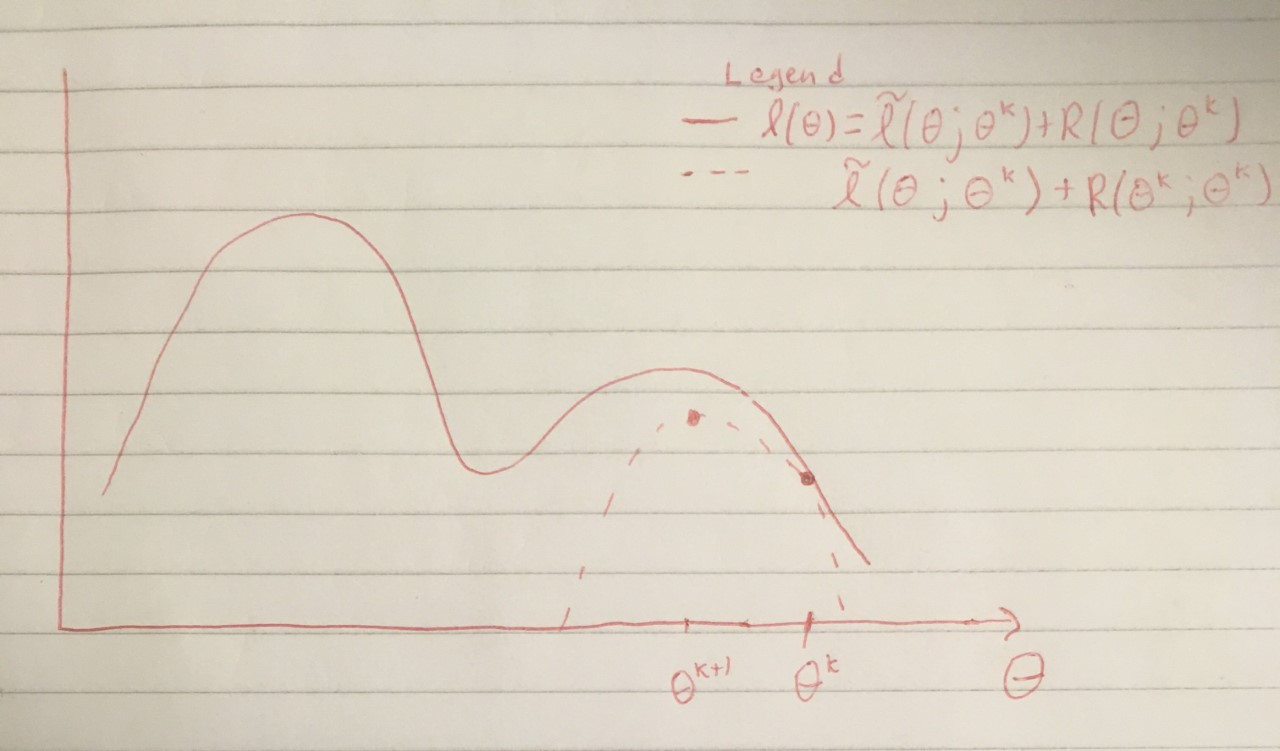
\includegraphics[scale=0.5]{EMv2.png}
% \caption{A visualization of an EM step. In the E-step we compute the dotted curve based on the current values of the parameter $\theta^k$ (up to an additive constant). The dotted curve is guaranteed to lie beneath the log-likelihood and to intersect the log-likelihood curve at $\theta^k$. In the M-step we find a point $\theta^{k+1}$ maximizing the dotted curve. The log-likelihood at $\theta^{k+1}$ is guaranteed to be at least as large as that evaluated at $\theta^k$ because both the value of the dotted curve and the gap between the solid and dotted curve will increase (or at least not decrease).}
% % \end{figure}

% By the above remarks, we see that the EM algorithm is an ascent method; {\bf the likelihood increases at each step}.


% \newpage
% \section{Cross-Validation}

Cross-Validation is a topic that arises frequently in the applied qualifying exam. Occasionally complete questions are dedicated to cross validation, other times it is a subpart.

Typically, cross validation is used to achieve one or both of the following,
\begin{enumerate}
\item \textbf{Model selection:} This can be to choose between a few different model choices or to pick the values of tuning parameters, with the goal of selecting the model that will have the highest prediction accuracy.
\item \textbf{Accuracy assessment:} Estimating the accuracy of the prediction model that is trained.
\end{enumerate}

We will describe what cross-validation is and to what extent it meets the above two goals. Next, we will then describe a few issues with using cross-validation that have come up in previous quals and some suggested workarounds.

\subsection{Cross-validation for model selection or parameter tuning}\label{sec:CVmodelSelection}

The most straightforward quals questions about cross-validation, simply ask you how you would pick certain tuning parameters in the model or how would you pick the best model among a collection of models (see Question 5d on the 2012 Qual as well as Question 5c on the 2015 Qual). If there is a prediction task of interest a good way to pick the best model is cross-validation. In particular suppose you have $n$ data points $\big( (X_i,Y_i )  \big)_{i=1}^n$ where $X_i$ are the features and $Y_i$ are the outcomes you'd like to predict.

To perform $K$-fold cross validation, randomly split the data into $K$ folds of size roughly $n/K$ (often $K$ is chosen to be 5 or 10). Let $\kappa: \{1,2,\dots, n \} \to \{1,\dots,K \}$ be the function such that takes a sample $i$ to its fold $\kappa(i)$. Now let $\theta$ be parameter vector that embeds all the tuning parameters (model class choices can be considered categorical tuning parameters). Also for $k \in \{1,\dots,K \}$ let $\hat{f}_{-k}( \cdot; \theta)$ denote the model for predicting for $Y$ that is trained on all folds except the $k$th fold when the tuning parameters are set to $\theta$. Finally, let $\ell$ is some loss function for the prediction error (often it is chosen to be squared error loss when $Y$ is a continuous variable, and 0-1 loss when $Y$ is categorical). The cross-validation error is given by $$\widehat{\text{Err}}^{\text{(CV)}}(\theta) = \frac{1}{n} \sum_{i=1}^n \ell \Big( Y_i, \hat{f}_{-\kappa(i)}( X_i; \theta) \Big).$$ 
Then to pick optimal tuning parameters you could simply select the $\theta$ that minimizes  $\widehat{\text{Err}}^{\text{(CV)}}(\theta)$. (Another common choice is to select the $\theta$ corresponding to lowest model complexity among $\theta$ values for which  $\widehat{\text{Err}}^{\text{(CV)}}(\theta)$ is within one standard error of $\inf_{\theta'} \widehat{\text{Err}}^{\text{(CV)}}(\theta')$). 

Given $\theta^* = \argmin \widehat{\text{Err}}^{\text{(CV)}}(\theta)$, we fit our model on the full data set $\{(X_i,Y_i)\}_{i=1}^n$, giving a model $\hat{f}(\cdot;\theta^*)$ that we can deploy.

\subsection{Cross-validation for accuracy assessment}

Suppose we want to assess how accurate a prediction method is, but we need not select any tuning parameters or conduct model selection. We can also assess the accuracy of the model using $K$-fold cross validation. This simply involves running the procedure described in the previous subsection for the prespecified choice of $\theta$ and computing $$\widehat{\text{Err}}^{\text{(CV)}} = \frac{1}{n} \sum_{i=1}^n \ell \Big( Y_i, \hat{f}_{-\kappa(i)}( X_i;\theta) \Big),$$ where $\kappa(i)$ and $\hat{f}_{-k}(\cdot;\theta)$ are as above. 

While $\widehat{\text{Err}}^{\text{(CV)}}$ seems like a reasonable way to measure the error associated with the prediction method, it is not immediately obvious what quantity $\widehat{\text{Err}}^{\text{(CV)}}$ estimates. Let's look at two reasonable guesses.

Suppose that $ \{(X_i,Y_i) \}_{i=1}^{n+1}$ are IID and let $\mathcal{T} =  \{(X_i,Y_i )\}_{i=1}^{n}$ denote the training data and let $\hat{f}_{\mathcal{T}}(\cdot)$ denote the prediction model trained on the training data $\mathcal{T}$. Two reasonable guesses for what $\widehat{\text{Err}}^{\text{(CV)}}$ estimates are 

\begin{align*}\text{Err}_{\mathcal{T}}& = \mathbb{E} \Big[ \ell \Big( Y_{n+1} , \hat{f}_{\mathcal{T}}(X_{n+1}) \Big) \mid \mathcal{T} \Big], \ \text{and}\\
     \text{Err}_n &= \mathbb{E}[\text{Err}_{\mathcal{T}}] = \mathbb{E} \Big[ \ell \Big( Y_{n+1} , \hat{f}_{\mathcal{T}}(X_{n+1}) \Big)\Big].
\end{align*}

The quantity $\text{Err}_{\mathcal{T}}$ is the expected loss on a new test point, conditional on the training data (the expectation is only over $X_{n+1}$ and $Y_{n+1}$). On the other hand $\text{Err}_n$ is the expected loss of predicting on a new point when training on $n$ randomly sampled points (the expectation is taken over $X_{n+1},Y_{n+1}$ and $\mathcal{T}$). It turns out that $\widehat{\text{Err}}^{\text{(CV)}}$ is a good estimator for $\text{Err}_n$, but unfortunately is a poor estimator of $\text{Err}_{\mathcal{T}}$ (See Chapter 7.12 in \cite{hastie2009elements} and \cite{Bates2022CrossVal} for simulation-based and theoretical arguments supporting this claim).

Now that we've established that $\text{Err}$ is the estimand for cross-validation, we can discuss Quals questions which ask whether Cross-Validation is downward biased or upward biased. In Question 2 of the 2015 Qual, it asks whether cross-validation is upward or downward biased for estimating prediction error (in a setting with IID data and no tuning parameters). The answer is that it is upward biased because 

\begin{align*}
    \mathbb{E} \big[ \widehat{\text{Err}}^{\text{(CV)}}  \big] &= \frac{1}{n} \sum_{i=1}^n \mathbb{E} \Big[ \ell \Big( Y_i, \hat{f}_{-\kappa(i)}( X_i) \Big) \Big] \\
    &= \frac{1}{n} \sum_{i=1}^n \text{Err}_{\#\{j : \kappa(j) \neq \kappa(i)\}}\\
    & >  \frac{1}{n} \sum_{i=1}^n  \text{Err}_n\\
    & =  \text{Err}_n,
\end{align*}    
The inequality holds because for any reasonable prediction algorithm the expected error strictly decreases as the sample size grows. Thus, $\widehat{\text{Err}}^{\text{(CV)}}$ is upward biased for the expected error when training on a dataset the size of the full dataset. 

\subsubsection*{The number of folds}

Suppose that each fold has exactly $m = n/K$ data points. The bias in $\widehat{\text{Err}}^{(\text{CV})}$ is then equal to $\text{Err}_{n-m} - \text{Err}_{n} > 0$. This bias would decrease as $m$ goes to $0$. If we want to make this bias as small as possible, then we should take $K=n$ folds. This is called \emph{leave one out (LOO)} cross validation. For many models, leave one out cross validation is not tractable because we have to perform $n$ model fits. However, for simple models like linear models fit with OLS there are computational tricks which make it possible to calculate the leave one out cross validation error without fitting $n$ models. 

Another consideration is the variance of $\widehat{\text{Err}}^{\text{(CV)}}$. If we have $K \approx n$, then we would expect the fitted model $\hat{f}_{-k}(\cdot)$ to be highly correlated since they were all trained on essentially the same data. Thus, picking the number of folds involves a bias-variance trade-off. The values $K=5$ or $K=10$ are usually taken as defaults, see Section 7.10 of \citep{hastie2009elements} for more details.


\subsection{Nested Cross-validation}

There are some quals questions, where you have to \textit{both} conduct model selection (or parameter tuning) and conduct accuracy assessment for the entire procedure, including model selection (see Question 5 on the 2013 exam and Question 2 on the 2018 exam). In these questions you have to be careful to make sure that the data used for accuracy assessment was not used in the model selection process. If you use select the $\theta^*$ minimizing $\widehat{\text{Err}}^{\text{(CV)}}(\theta)$, then $\widehat{\text{Err}}^{\text{(CV)}}(\theta^*)$ could grossly underestimate the prediction error on new data of the full training procedure (which includes model selection/parameter tuning).


Ideally if you want to use cross-validation to tune parameters or perform model selection, you should not use the same training data to assess accuracy, and instead you should use a held out test set to assess accuracy. In particular, you should do model selection on the training set using cross-validation (see Section \ref{sec:CVmodelSelection}), train the selected model on the full training set, and assess accuracy on some held out test set. Unfortunately, sometimes your data set is so small that it would be overly wasteful to hold out a separate test set (e.g. in Question 2 on the 2018 exam). Luckily one can use nested cross-validation if they want to use all the data for both model selection and accuracy assessment without grossly underestimating the prediction error.

The nested cross-validation procedure can be described by the following steps:
\begin{enumerate}
\item Conduct model selection on the full dataset using cross validation (as in Section \ref{sec:CVmodelSelection})
\item Let $\theta^*$ be the model selected in the previous step. Train a prediction $\hat{f}(\cdot ; \theta^*)$ on your entire dataset. Return $\hat{f}(\cdot ; \theta^*)$ as your final prediction function.
\item Randomly split the data into $K$-folds, let $\kappa: \{1,2,\dots, n \} \to \{1,\dots,K \}$ be such that $\kappa(i)$ gives the fold that sample $i$ is assigned to. 
\item For each $k=1,\dots,K$, remove the data from the $k$th fold and on this smaller dataset (of size $n(K-1)/K$ samples) run the cross-validation procedure (as described in Section \ref{sec:CVmodelSelection}) to select the best $\theta$. Let $\theta_{-k}^*$ denote the parameters for the best model selected on the dataset when the $k$th fold was removed.
\item For each $k=1,\dots,K$,  train a prediction function $\hat{f}_{-k}(\cdot ; \theta_{-k}^*)$ on all of your data except the $k$th fold. Store the prediction function $\hat{f}_{-k}(\cdot ; \theta_{-k}^*)$.
\item Calculate and return the following estimate for the prediction error $$\widehat{\text{Err}}^{\text{(Nested CV)}} =  \frac{1}{n} \sum_{i=1}^n \ell \Big( Y_i, \hat{f}_{-\kappa(i)}( X_i; \theta_{-\kappa(i)}^*) \Big).$$

\end{enumerate}



Note that the first two steps conduct model selection and train the final prediction model which is what will be deployed. Steps 3-6 are for assessing accuracy of the \textit{full} procedure.

\subsection{Cross-validation with dependent samples}

Cross-validation can give an overoptimistic accuracy assessment when there are strong temporal or spatial correlations between the samples. It can also lead to selecting models that don't generalize well to new spatial locations or time periods. One extreme example that illustrates this phenomena, is to consider the $1$-nearest neighbors prediction algorithm in setting where both the features $X$ and the outcome $Y$ have high spatial (or temporal) correlations. If we use naive cross-validation to assess the accuracy, it is likely that many points in each held out fold have a point in the non-held-out training folds that is nearby in space (or time). Because such a nearby point in space (or time) is likely to have similar $X$ and $Y$ values due to strong spatial (or temporal) correlations, taking the $Y$ value of the nearest neighbor feature space would give a very accurate prediction. However, we are interested to estimate the accuracy of $1$-nearest neighbors on new data, that is not near the training data in space, so naive cross-validation will be overly optimistic. If the goal is model selection rather than accuracy assessment, having pairs of points in separate folds with high correlations can incentivize the model being selected to rely too heavily on artifacts or features that are highly correlated in space (or time) but do not matter for predicting new independent samples.

For settings in which there are strong temporal or spatial correlations between the samples, if we wish to ultimately assess the accuracy of predictions at new time periods or locations, we should instead run grouped cross-validation. In particular, we should assign points that are highly correlated with each other into the same group, and when running cross-validation, we should ensure that points within the same group are within the same fold. Ultimately, we would like to construct folds that have as little correlation between pairs of points in different groups as possible (having correlated points in the same fold is ok). 

This has come up in a couple of Quals questions in the past. In Question 6 of the 2011 Qual, the points are likely to be spatially correlated, so to assess the accuracy of the classifier with cross-validation we should make sure that points which are geographically close to each other end up in the same fold. In Question 4 part 1 of the 2014 Qual, the points are likely to be temporally correlated, so to conduct model selection with cross-validation, we should make sure that the folds contain consecutive years to minimize the correlation between pairs of samples in different folds.

One final note is that by the same reason, we should be careful about using cross-validation nested within a bootstrap procedure. Bootstrap involves sampling the data with replacement, so if cross-validation for model selection is conducted on the data sampled with replacement, it is possible that two different folds will have the same data point. This can be problematic.

\subsection{Making sure model fit on training folds is well-defined}

In some settings where you want to run cross-validation, it may not be a guarantee that the model can be properly fit on a subset of the data of size $n(K-1)/K$ samples. For example, in question 5b in the 2014 Qual, you have to use cross-validation to select the number of tiers to include in the model; however, the given model cannot be tested on each held out fold if any of the teams appear only in one fold. Thus, you should randomly regenerate the $K$-folds until the $K$-folds do not have this issue. 

Another setting where this might come up is if you want to fit a Bradley--Terry model with a tuning parameter to predict the outcome of games. A Bradley--Terry model can only be fit when the graph with teams as nodes and games as edges is fully connected. It is possible that the (Teams, Games) graph will be fully connected for the full dataset with $n$ games, but on some subsets of the data with only $n(K-1)/K$ games, the  (Teams, Games) graph will not be fully connected. In such a setting you can try regenerating the folds until all training subsets under consideration have fully connected (Teams, Games) graphs. 

% \newpage 
% \section{Linear Models: Additional topics}

In this section we will touch on three topics that relate to the linear model and may come up on the exam.

\subsection{ANOVA}

\subsubsection*{F-test revisited}

The word ANOVA can be used to refer to a number of things. It is an abbreviation of analysis of variance and is sometimes used to refer to $F$-test for model comparison. Recall that in  Section \ref{sec:F-test}, we had the model,
\[Y = X_1\beta_1 + X_2\beta_2 + \varepsilon, \]
and we wanted to test $\mathcal{H}_0: \beta_2 = 0$. Our test-statistic was,
\[F = \frac{\vert \vert  \hat{Y}_f -\hat{Y}_1  \vert \vert_2^2/p_2}{\vert \vert Y - \hat{Y}_f  \vert \vert_2^2/(n-p_1-p_2)}, \]
which can be written as,
\[F =  \frac{(\vert \vert  Y -\hat{Y}_1  \vert \vert_2^2 - \vert \vert Y - \hat{Y}_f \vert \vert_2^2 )/p_2}{\vert \vert Y - \hat{Y}_f  \vert \vert_2^2/(n-p_1-p_2)}. \]
The term $\vert \vert Y-\hat{Y}_1 \vert \vert_2^2$ is an estimate of the error variance in the full model and $\vert \vert Y-\hat{Y}_1 \vert \vert_2^2$ is an estimate of the error variance in the sub-model. The $F$-test compares these two estimates and rejects the null hypothesis if $\vert \vert Y - \hat{Y}_1 \vert \vert_2^2$ is sustainably larger than $\vert \vert Y-\hat{Y}_f \vert \vert_2^2$. Thus, the $F$ test is an ``analysis of variance.''

\subsubsection*{ANOVA Models}

The word ANOVA is also used to describe linear models with only categorical features. In these models, the categorical features divide the observations into $K$ groups. The inferential goal is to detect differences between the groups. This often done using the $F$-test (aka an analysis of variance).

\subsubsection*{Single Factor}

The simplest version of ANOVA is where there is a single categorical feature. Suppose the feature can take $I$ values, and our each value $1\le i \le I$, we have observations $Y_{i,s}$ for $1\le s \le n_i$. The ANOVA model is,
\begin{equation}\label{ANOVA1}
    Y_{i,s} = \mu + \alpha_{i} + \varepsilon_{i,s}, 
\end{equation}
with $\varepsilon_{i,s} \simiid \mathcal{N}(0,\sigma^2)$ for $1 \le i \le I$ and $1 \le s \le n_i$. The parameter $\mu$ is the grand mean and $\alpha \in \reals^I$ is a vector of off-sets. As written, the model above is not identifiable. If we let $\ones_I$ denote the length $I$ vector of all ones, then we could add a constant $\nu$ to $\mu$ and subtract $\nu\ones_I$ from $\alpha$ and the distribution of $Y$ will be unchanged. To make the model identifiable, constraints are added to parameters $(\mu,\alpha)$. There are three common approaches,
\begin{itemize}
    \item Set $\alpha_1 = 0$. This is what \verb|R| does when use \verb|lm| with a categorical feature. This constraint makes the most sense when category 1 is a ``baseline'' category. The other parameters $\alpha_i, i > 1$ tell you how the mean differs in category $i$ compared to category $1$.
    \item Require $\sum_{i=1}^I \alpha_i = 0$. This has the nice theoretical property that $\alpha^\top \ones_I = 0$. Thus, the vector of parameters $\alpha$ is orthogonal to any constant vector $\mu \ones_I$. This can simplify calculations. In this model $\alpha_i$ measures the difference between the mean of group $i$ and the grand mean.
    \item Require $\mu = 0$. In this model $\alpha_i$ is simply the mean of group $i$.
\end{itemize}
Each of these constraints are one-dimensional and any of them make $(\mu,\alpha)$ identifiable. The degrees of freedom for the model \eqref{ANOVA1} is $I$. Regardless of the constraint choice, the group means $\mathbb{E}[Y_{i,s}] = \mu + \alpha_i$ are unchanged. The parameters can be fit using constrained least-squares. Under any of the constraints, the fitted values are always the same,
\[\hat{Y}_{i,s} = \hat{\mu}+\hat{\alpha}_i = \frac{1}{n_i}\sum_{s=i}^{n_s} Y_{i,s} = \bar{Y}_{i,+}. \]
The difference between two groups are also unchanged,
\[\hat{\alpha}_{i}-\hat{\alpha}_{i'} = \bar{Y}_{i,+} - \bar{Y}_{i',+}. \]

\subsubsection*{Testing}

To test for a difference between groups, we can use the $F$-test to test $\mathcal{H}_0 : \alpha_1 = \cdots = \alpha_I$. The fitted values in the full model are $\hat{Y}_{i,s}^{\text{full}} = \bar{Y}_{i,+}$. Under the null, the fitted values are 
\[\hat{Y}_{i,s}^{\text{null}} = \bar{Y}_{+,+} = \frac{1}{n_{+,+}} \sum_{i=1}^I \sum_{s=1}^{n_i} Y_{i,s},\] 
where $n_{+,+} = \sum_{i=1}^I n_{i}$ is the total number of observations. 

We can also use a t-test to test for a difference between the groups ``in a direction.'' A contrast is any vector $c \in \reals^K$ with $\sum_{i=1}^I c_i = 0$. Under $\mathcal{H}_0$, we have $c^\top \alpha =0$ for any contrast $c$. Common choice of $c$ are pairwise difference $c= e_i-e_{i'}$ or the difference between two subgroups $c = \frac{1}{I_1}\sum_{i=1}^{I_1}e_i - \frac{1}{I-I_1}\sum_{s=I_1+1}^I e_i$ for $1 < i < I$. When testing contrast you need to be careful about multiple testing issues. Your contrasts should not be data dependent, and you have to correct for multiplicity if you do test multiple contrasts.

\subsubsection*{Multiple factors}

The previous section can easily be extended to handle multiple features. For simplicity, we will only discuss two-factor models. Suppose one feature has $I$ levels and the other has $J$ levels. Suppose that in group $i,j$ we have observations $Y_{i,j,s}$ for $1\le s \le n_{ij}$. The ANOVA model \emph{without interactions} is,
\begin{equation}
    \label{ANOVA2} Y_{i,j,s} = \mu + \alpha_i + \beta_j + \varepsilon_{i,j,s}
\end{equation}
which has $1 + I + J$ parameters but only $I+J-1$ degrees of freedom. I find it useful to think of the parameters as matrices in $\reals^{I\times J}$. We have a constant matrix $\mu \ones_I \ones_J^\top $, a matrix with constant rows $\alpha \ones_{J}^\top$ and a matrix with constant columns $\ones_I \beta^\top$. 
To make this model identifiable, the typical constraints are,
\begin{itemize}
    \item $\alpha_1 = 0$ and $\beta_1 = 0$. Here again we are treating $i=1, j=1$ as a baseline category.
    \item $\sum_{i=1}^I \alpha_i = 0$ and $\sum_{j=1}^H \beta_j = 0$. Here there is no baseline category and $\alpha_i + \beta_j$ is the difference in mean between category $(i,j)$  and the grand mean. Here again we have orthogonality between the matrices $\mu \ones_I \ones_J^\top $, $\alpha \ones_{J}^\top$ and $\ones_I^\top \beta$.
\end{itemize}
Under all of these models the fitted values of $Y$ are,
\[\hat{Y}_{i,j,s} = \bar{Y}_{i,+,+}+\bar{Y}_{+,j,+} - \bar{Y}_{+,+,+}, \] 
where $\bar{Y}_{i,+,+}$ is the average value of $Y_{i,j',s'}$ over $j'$ and $s'$, $\bar{Y}_{+,j,+}$ is the average value of $Y_{i',j,s'}$ over $i'$ and $s'$, and $Y_{+,+,+}$ is the grand average over all values of $Y$. From here you can work out $\hat{\mu},\hat{\alpha}$ and $\hat{\beta}$ under the different constraints.

We can also make a two-factor model with interactions,
\begin{equation}
    \label{ANOVA3} Y_{i,j,s} = \mu + \alpha_i + \beta_j + \gamma_{ij} + \varepsilon_{i,j,s},
\end{equation}
which has $1+I+J+IJ$ parameters but only $IJ$ degrees of freedom. Again it is helpful to think of the parameters $\mu,\alpha,\beta$ and $\gamma$ as living in $\reals^{I\times J}$. To make the parameters identifiable we need $1+I+J$ constraints. The two common choices are
\begin{itemize}
    \item $\alpha_1 = 0$, $\beta_1=0$, for all $j$ $\gamma_{1,j}=0$ and for all $i$ $\gamma_{i,1}=0$ (note that the constraint $\gamma_{1,1}=0$ is counted twice.)
    \item $\sum_{i=1}^I \alpha_i = 0$, $\sum_{j=1}^J \beta_j = 0$, for all $i$ $\sum_{j=1}^J\gamma_{i,j}=0$ and for all $j$ $\sum_{i=1}^I \gamma_{i,j} = 0$ (note that one of the constraints are redundant). These constraints imply that $\mu \ones_I \ones_J^\top $, $\alpha \ones_J^\top$, $\ones_I \beta^\top$ and $\gamma$ are all orthogonal in $\reals^{I \times J}$.
\end{itemize}
The fitted values here are $\hat{Y}_{i,j,s} = \bar{Y}_{i,j,+}$ the average value of $Y_{i,j,s'}$ over $s'$. From here you can work out $\hat{\mu},\hat{\alpha},\hat{\beta}$ and $\hat{\gamma}$. Again the F and t-tests can be used to compare groups. 


\subsection{Generalized least squares\footnote{Not to be confused with GLMs!}}

In ordinary least squares, we have the linear model,
\begin{equation}\label{GLS:model}Y = X \beta + \varepsilon, \end{equation}
where $\varepsilon$ has mean zero and covariance $\sigma^2 I$. The corresponding OLS estimator of $\beta$ is $\hat{\beta}= (X^\top X)^{-1}X^\top Y$. In \emph{generalized least squares} we replace the assumption $\cov(\varepsilon) = \sigma^2 I$ with the assumption $\cov(\varepsilon) = \Omega$ where $\Omega$ is a \emph{known} non-singular covariance matrix. The GLS estimator is given by
\begin{align*}
    \hat{\beta}_\Omega &= \argmin_\beta (Y-X^\top \beta)^\top \Omega^{-1} (Y-X^\top \beta)\\
    &=(X^\top \Omega^{-1} X)^{-1} X^\top \Omega^{-1}Y.
\end{align*}
If $\varepsilon \sim \mathcal{N}(0,\Omega)$, then $\hat{\beta}_{\Omega}$ is the MLE for $\beta$. One way to derive the equation of $\hat{\beta}_\Omega$ is by multiplying \eqref{GLS:model} on the left by $\Omega^{-1/2}$ (which exists since $\Omega$ is non-singular and positive semi-definite). This gives the model,
\[\widetilde{Y} = \widetilde{X}\beta + \widetilde{\varepsilon}, \]
where $\widetilde{Y}=\Omega^{-1/2}Y$, $\widetilde{X} = \Omega^{-1/2}X$ and $\widetilde{\varepsilon} = \Omega^{-1/2}\varepsilon \sim (0,I)$. Thus, we have a standard OLS model with a transformed response and feature matrix. The OLS estimate for the transformed model is
\[(\widetilde{X}^\top \widetilde{X})^{-1}\widetilde{X}^\top \widetilde{Y} = (X^\top \Omega^{-1}X)^{-1}\Omega^{-1}Y, \]
which is exactly $\hat{\beta}_\Omega$. 


\subsubsection*{Weighted least squares}

It is unlikely that we will know $\Omega$ exactly and thus generalized least squares doesn't come up that often. An exception is the special case \emph{weighted least squares}. Here we assume that $\varepsilon_i$ are independent and mean zero but with different variances. That is we assume,
\[ \cov(\varepsilon) = \sigma^2W,\]
where $W \in \reals^{n \times n}$ is a known diagonal matrix and $\sigma^2$ is unknown. That is, we don't know the exact covariance matrix of $\varepsilon$, but we know that $\varepsilon_i$ are uncorrelated and the variance of $\varepsilon_i$ is proportional to $W_{ii}$. This formulation is useful because the unknown parameter $\sigma^2$ will cancel out in the calculation of $\hat{\beta}_\Omega$. Weighted least squares often comes up in repeated sampling situations where $Y_i$ is an average of $n_i$ observations and $W_{ii} = \frac{1}{{n_i}}$. 



% \newpage 
% \section{Bayesian Modelling\footnote{Kenneth Tay, Stephen Bates, Dan Kluger and M.H.}}

\subsection{Overview}

In Bayesian inference we have unobserved parameters $\theta$ and observed data $X$. We have a probabilistic model for the joint distribution of $(\theta,X)$. Typically, this is typically presented as a prior on $\theta$ and a conditional distribution (or likelihood) on $X$ given $\theta$. That is
\begin{align*}
    \theta &\sim p(\theta) \quad \text{(prior)},\\
    X \mid \theta &\sim p(X\mid \theta) \quad \text{(likelihood)}.
\end{align*}
Our joint distribution is thus,
\[p(\theta,X) = p(\theta)p(X \mid \theta). \]
A primary goal in Bayesian modelling is to make inferences on $\theta$ based on the observed data $X$. This is typically done with respect to the \emph{posterior distribution} of $\theta$,
\begin{align*}
    p(\theta \mid X) &=\frac{p(\theta,X)}{\int_\Theta p(\theta',X)d\theta'}\\
    &=\frac{p(\theta)p(X \mid \theta)}{\int_\Theta p(\theta')p(X \mid \theta')d\theta'}
\end{align*}
The posterior distribution on $\theta$ captures all the information (assuming our model) about $\theta$ in $X$. This includes uncertainty in $\theta$. Many quantities of interest can be expressed as functional of the posterior distribution $p(\theta \mid X)$. Common examples are:
\begin{itemize}
    \item The posterior mode or MAP of $\theta$, $\argmax_\theta p(\theta \mid X)$, another point estimate for $\theta$.
    \item The posterior mean of $\theta$, $\bbE[\theta \mid X]$ which is a point estimate for $\theta$.
    \item The posterior variance of $\theta$ or the posterior expectation of a function $h(\theta)$, $\bbE[g(\theta)\mid X]$.
    \item The quantiles of the posterior distribution which provide a ``credible set'' for the values of $\theta$.
\end{itemize}

Broadly speaking, there are two types of quals questions about Bayesian modelling that I think could come up. 
\begin{enumerate}
    \item You are given a description of some data, and you're asked to describe a Bayesian model for the data. In this question describing the model would be the main part of the question and you would only need to sketch how you would do inference. This would be ``Type J''.
    \item You are given a model and are asked to do some calculations related to doing inference. This would be ``Type C''. Typical tools are conjugacy, EM, MCMC and CAVI.
\end{enumerate}

\subsection{Describing a model}

The notation 
\[p(\theta,X) = p(\theta)p(X \mid \theta), \]
hides a lot of possible complexity. Bayesian modelling is very flexible and can easily account for complicated relationships between your parameters $\theta$ and your data $X$. A typical example of this is \emph{hierarchical modelling} where the distribution of some parameters depend on others. Here DAGs are a powerful tool. Let's consider a concrete example.

\subsubsection*{Binomial hierarchical model}

Suppose we want to make inference on a proportion $\theta$ where our data follows $X \sim \mathrm{Binom}(n,\theta)$. A natural prior in this case is the beta distribution $\theta \sim \mathrm{Beta}(\alpha,\beta)$ where $\alpha,\beta$ are fixed hyper-parameters. The posterior distribution of $\theta \mid X$ is $\mathrm{Beta}(\alpha + X,\beta + (n-X))$. 

Here the hyperparameters $\alpha,\beta$ were considered fixed. In theory, hyperparameters will be based on genuine prior knowledge from previous experiments. However, if we have $J$ samples $X_j \sim \mathrm{Binom}(n_j,\theta_j)$, then we can put priors on $(\alpha,\beta)$ and ``pool'' our estimation of $(\theta_1,\ldots,\theta_J)$ across the $J$ samples. One model would be,

\begin{align*}
    \alpha, \beta &\simiid \mathrm{Gamma}(5,1),\\
    \theta_j\mid \alpha,\beta &\simiid \mathrm{Beta}(\alpha,\beta),\\
    X_j \mid \theta_j & \simind \mathrm{Binom}(n_j,\theta_j). 
\end{align*}
The choice of a Gamma distribution here is arbitrary. You could use any other distribution supported on $[0,\infty)$. In the hierarchical model, we want to make inference on the full posterior,

\[p(\theta,\alpha,\beta \mid X) \propto p(\alpha,\beta)p(\theta\mid \alpha,\beta)p(X \mid \theta,\alpha,\beta).\]

Unlike the case when $\alpha$ and $\beta$ where fixed, the above won't have a closed form and so you'll have to perform one of the approximations described below.

\subsection{Inference}

\subsubsection*{Conjugacy}

To find a posterior distribution, you can ignore all factors that don't depend on the parameters $\theta$ since these we will be integrated out. Thus, you should have a list of distributions and try to pattern match your posterior with one of the known distributions. It is also very helpful to have a list of moments for different distributions. These can be very helpful when calculating posterior expectations.

\subsubsection*{EM}

The EM algorithm can be used to find the posterior mode $\hat{\theta}_{MAP} = \argmax_{\theta}p(\theta\mid X)$. This algorithm is likely to come up and is often used in latent variable models. See Section \ref{sec:review_EM}

\subsubsection*{MCMC}

Markov Chain Monte Carlo (MCMC) is a general purpose tool for sampling from posteriors. It can be used calculate posterior expectations and approximate $p(\theta \mid X)$. Two general purpose MCMC samplers are the ``Gibbs sampler'' and ``Metropolis--Hastings''. These samplers aren't used in modern Bayesian modelling software but you might get asked calculation questions about them. Both algorithms gennerate samples $\theta^1,\theta^2,\ldots,\theta^S$ such that for sufficiently large $s$, $\theta^s \sim p(\theta \mid X)$. These samples are then used to estimate posterior expectations

\begin{equation}\label{eq:MCMC-est} \bbE[h(\theta)\mid X] \approx \frac{1}{S}\sum_{s=1}^S h(\theta^s).\end{equation}
The Gibbs sampler is based on the conditional distributions $p(\theta_j \mid \theta_{-j},X)$ where $\theta_j$ is one coordinate of the vector $\theta \in \reals^d$ and $\theta_{-j} \in \reals^{d-1}$ are the remaining coordinates. The Gibbs sampler proceeds as follows,

\begin{enumerate}
    \item Initialize at some $\theta^0 \in \reals^d$.
    \item For $s=1,\ldots,S$,
    \begin{enumerate}
        \item Let $j \in \{1,\ldots,d\}$ be such that $j=s \bmod d$.
        \item Draw $\theta_j^{\mathrm{new}}$ from $p(\theta_j \mid \theta_{-j}^{s-1},X)$. 
        \item Set,
        \[ \theta_i^s = \begin{cases}
            \theta_j^{\mathrm{new}} & \text{if } i = j,\\
            \theta_i^{s-1} & \text{if } i \neq j. \end{cases}\]
    \end{enumerate}
\end{enumerate}
The algorithm as described above is called the \emph{systematic scan Gibbs sampler},
as we update  the $d$ coordinates in order systematically. The \emph{random scan Gibbs
sampler} replaces step 2(a) with $j \sim \mathrm{Unif}(\{1,\ldots,d\})$. 

The \emph{Metropolis--Hasting algorithm}\footnote{Although there is a case that is should be called the Rosenbluth--Hasting algorithm \url{https://youtu.be/rZk2FqX2XnY?t=1276}} requires a proposal distribution $q(\theta;\theta^{\mathrm{old}})$ which we can sample from. It proceeds as follows,
\begin{enumerate}
    \item Initialize at some $\theta^0 \in \reals^d$.
    \item For $s=1,\ldots,S$,
    \begin{enumerate}
        \item Sample a proposal $\theta^* \sim q(\theta;\theta^{s-1})$.
        \item Let $\alpha = \frac{p(\theta^*\mid X)q(\theta^*;\theta^{s-1})}{p(\theta\mid X)q(\theta^{s-1};\theta^*)}$. Then set,
        \[\theta^s = \begin{cases}
            \theta^* &\text{with probability } \min\{1,\alpha\},\\
            \theta^{s-1}&\text{with probability } 1-\min\{1,\alpha\}.
        \end{cases} \]
    \end{enumerate}
\end{enumerate}



% \newpage
% \section{CAVI}\label{sec cavi}

\subsection{Variational inference}

Variational inference is another approach to Bayesian inference. Like MCMC, variational inference approximates the posterior $p(\theta|X)$. Variational inference uses optimization instead of sampling. Methods like MCMC that are based on sampling asymptotically unbiased. That is, given long enough runs of the chain we will draw samples from the exact posterior distribution $p(\theta | X)$. However, the MCMC estimate \eqref{eq:MCMC-est} will always have variance which can dominate the error in estimating posterior expectations. At a high level, variational inference is another way of estimating $p(\theta | X)$ which trades off some of this variance for bias. 

The idea is that we will approximate the distribution $p(\theta| X)$ with a family of more tractable distributions $\{q(\theta) : q \in \mathcal{Q}\}$. We want to find $q^* \in \mathcal{Q}$ that is ``closest'' to $p(\theta |  X)$. A classical variational method is the ``Laplace approximation'' where $\mathcal{Q}$ is the set of multivariate Gaussian. And $q^*$ is found by a Taylor's approximation at the MAP. 

A more modern approach is coordinated ascent variational inference (CAVI). Here $\mathcal{Q}$ is a set of probability distributions that factor into independent components. The distance is KL divergence, 
\[\KLD{q(\theta)}{p(\theta | X)} = \bbE_q[\log q(\theta) ] - \bbE_q[\log p(\theta | X)].\]
Today we will focus derive the CAVI updates and go through an example.

\subsection{CAVI updates}


The CAVI optimization problem is to find $q^*$ where,
\[q^* = \argmin_{q \in \mathcal{Q}}\KLD{q(\theta)}{p(\theta | X)}.  \]
As written, this is intractable since evaluating $\KLD{q(\theta)}{p(\theta | X)}$ seems to require knowing $p(\theta | X)$. Fortunately, we can use the factorization $p(\theta | X) = \frac{p(\theta,X)}{p(X)}$ to rewrite $\KLD{q(\theta)}{p(\theta | X)}$ in the following way,
\begin{align}
    \KLD{q(\theta)}{p(\theta | X)}&=\bbE_q\left[\log q(\theta)\right] - \bbE_q\left[\log p(\theta | X) \right]\nonumber \\
    &=\bbE_q\left[\log q(\theta)\right]-\left(\bbE_q\left[\log p(\theta,X)\right] - \bbE_q\left[\log p(X)\right]\right)\nonumber \\
    &=-\underbrace{\left(\bbE_q\left[\log p(\theta,X)\right] - \bbE_q \left[\log q(\theta)\right]\right)}_{\text{ELBO}} + \underbrace{\log p(X)}_{\text{evidence}}.\label{eq:KLD}
\end{align}
We will call $\log p(X) = \log \left(\int_\Theta p(\theta,X)d\theta'\right)$ the \emph{evidence} and 
$$
\mathcal{L}[q] = \bbE_q\left[p(\theta,X)\right] - \bbE_q\left[\log q(\theta)\right]
$$ 
the \emph{evidence lower bound} or \emph{ELBO}. The takeaway of equation \eqref{eq:KLD} is
\begin{align*}
    q^* &=\argmin_{q \in \calQ} \KLD{q(\theta)}{p(\theta | X)}\\
    &=\argmin_{q \in \calQ} -\left(\bbE_q\left[\log p(\theta,X)\right] - \bbE_q \left[\log q(\theta)\right]\right)\\
    &=\argmax_{q \in \calQ} \mathcal{L}[q].
\end{align*}
So minimizing $\KLD{q(\theta)}{p(\theta |  X)}$ is the same as maximizing $\mathcal{L}[q]$. Since $\KLD{q(\theta)}{p(\theta | X)} \ge 0$ for all $q(\theta)$,  equation \eqref{eq:KLD} also implies that, 
\[\log p(X) = \KLD{q(\theta)}{p(\theta | X)} + \mathcal{L}[q] \ge \mathcal{L}[q], \]
so the ELBO is indeed a lower bound for the evidence.

We will now assume that we have a decomposition of $\theta$ into $J$ groups,
\[\theta = (\theta_1,\theta_2,\ldots,\theta_J). \]
We will also take $\calQ$ to be the set of distributions which factor into independent components over $(\theta_1,\theta_2,\ldots,\theta_J)$. That is $q \in \calQ$ if and only if we have
\[q(\theta) = \prod_{j=1}^J q_j(\theta_j), \]
for some distributions $q_j(\theta_j)$\footnote{The individual components $\theta_j$ need not be single scalar parameters. One $\theta_j$ could be a covariance matrix, another $\theta_j$ could be a vector of probabilities. You have a lot of flexibility in choosing the decomposition.}. We will write $\theta_{-j}$ for $\theta$ without the $j^{th}$ component and define $q_{-j}(\theta_{-j})$ by,
\[q_{-j}(\theta_{-j}) = \prod_{k \neq j}q_k(\theta_k). \]
We will now consider maximizing $\mathcal{L}[q]$ as a function of $q_{j}$ keeping $q_{-j}$ fixed. Recall that we have the factorizations,
\begin{align*}
    q(\theta)&=q_{-j}(\theta_{-j})q_j(\theta)\\
    p(\theta,X)&=p(X)p(\theta_{-j}|X)p(\theta_j |  \theta_{-j},X).
\end{align*}
Thus, writing $C_i$ for constants that do not depend on $q_{j}$, we have
\begin{align*}
    \mathcal{L}[q]&=\bbE_{q}[\log p(\theta,X)] - \bbE_{q}[\log q(\theta)]\\
    &=\bbE_q[\log p(X)] + \bbE_q[\log p(\theta_j  |  X)] + \bbE_{q}[\log p(\theta_j  |  \theta_{-j},X)]\\
    & - \bbE_{q}[\log q_{-j}(\theta_{-j})] - \bbE_{q}[\log q_j(\theta_j)]\\
    &=C_0 + \bbE_q[\log p(\theta_j |  \theta_{-j},X)] - \bbE_{q}[\log q_j(\theta_j)]\\
    &=C_0 - \left(\bbE_{q_{j}}[\log q_j(\theta_j)]-\bbE_{q_j}\left[\bbE_{q_{-j}}[p(\theta_j |  \theta_{-j},X)]\right]  \right)
\end{align*}
The term in the brackets is almost the KL-divergence between $q_{j}(\theta_{j})$ and another distribution on $\theta_{j}$. The only issue is that $\bbE_{q_{-j}}[p(\theta_j  |  \theta_{-j},X)]$ is not a normalized log-likelihood. Therefore, we define a distribution $\tilde{p}_j(\theta_j)$ by
\[\tilde{p}_j(\theta_j) \propto \exp\left(\bbE_{q_{-j}}[\log p(\theta_j  |  \theta_{-j},X)]\right). \]
Thus,
\[\mathcal{L}[q] = C_0 - \left(\bbE_{q_{-j}}[\log q_j(\theta_j)]-\bbE_{q_j}\left[\bbE_{q_{-j}}[p(\theta_j |  \theta_{-j},X)]\right]  \right) = C_1 - \KLD{q(\theta_j)}{\tilde{p}(\theta_j)}.  \]
Thus, to maximize $\mathcal{L}[q]$ as a function of $q_j$ we need to set $q(\theta_j)=\tilde{p}(\theta_j)$. Doing this iteratively for different values of $j$ gives the CAVI algorithm:
\begin{enumerate}
    \item Initialize $q$ at some distribution $q^0(\theta) = \prod_{j=1}^J q^0_j(\theta_j)$. 
    \item Set $s=0$
    \item Until $\mathcal{L}[q]$ converges:
    \begin{enumerate}
        \item Let $j \in \{1,\ldots, J\}$ be such that $j=s+1 \bmod J$.
        \item Define $\tilde{p}_j(\theta_j)$ by 
        \[\tilde{p}_j(\theta_j) \propto \exp\left(\bbE_{q_{-j}^s}[p(\theta_j |  \theta_{-j},X)]\right). \]
        \item Set,
        \begin{align*}
            q_j^{s+1}(\theta_j)&=\tilde{p}_j(\theta_j),\\
            q_{-j}^{s+1}(\theta_j)&=q_{-j}^s(\theta_{-j}).
        \end{align*}
        \item Set $s=s+1$.
    \end{enumerate}
\end{enumerate}

\subsection{CAVI for a qual question}

If you are asked to outline the steps of the CAVI algorithm for a particular model $p(\theta,X)$, this is what might be required.

\begin{enumerate}
    \item Calculate the conditionals $p(\theta_j  |  \theta_{-j},X)$. Hopefully you will be able to recognize them as a common family of distributions. If $p(\theta_j  |  \theta_{-j},X)$ is from a common family, then take $q(\theta_j)$ to be from that same family. 
    \item Calculate the expectation $\bbE_{q_{-j}^{\text{old}}}[\log p(\theta_j  |  \theta_{-j},X)]$. These tips can help,
    \begin{enumerate}
        \item The expectation is with respect to $\theta_{-j}$ so $X$ and $\theta_j$ are constants.
        \item You can drop additive terms that do not depend on $\theta_j$. These will cancel out when we normalize to define $\tilde{p}_j$.
        \item The term $\bbE_{q_{-j}^{\text{old}}}[\log p(\theta_j  |  \theta_{-j})]$ will often include terms which are the expectation of sufficient statistics in an exponential family. You can use Wikipedia tables to look these up or differentiate the CGF to calculate them.
    \end{enumerate}
    \item Define $q_j^\text{new}(\theta_j) \propto \exp\left(\bbE_{q_{-j}^{\text{old}}}\left[\log (\theta_j  |  \theta_{-j},X)\right]\right)$. Hopefully, $q_j^\text{new}$ will be from the same common family of distributions as $p_j(\theta_j  |  \theta_{-j},X)$.
    \item Calculate the ELBO $\mathcal{L}[q]$. Typically, $\mathcal{L}[q]$ can be written as a sum over the $J$ components from your decomposition of $\theta$. You can leave these terms as integrals or as KL-divergences between known distributions.
\end{enumerate}

\subsection{Example}

We will consider a simple Gaussian mixture similar to \ref{sec:MT}. Specifically, consider the following Bayesian model,
\begin{align*}
    \pi & \sim \mathrm{Beta}(\alpha,\beta)\\
    \mu & \sim \calN(\eta_1, \sigma_1^2)\\
    Z_n  |  \pi & \sim \mathrm{Bern}(\pi) \text{ for } n =1,\ldots,N\\
    X_n  |  Z_n=1, \mu & \sim \calN(\mu, 1) \text{ for } n = 1,\ldots,N\\
    X_n  |  Z_n=0, \mu & \sim \calN(0, 1) \text{ for } n = 1,\ldots,N.
\end{align*}
Our observed data are $X=(X_n)_{n=1}^N \in \reals^N$. The parameters $\mu$ and $\pi$ and the latent variables $Z=(Z_n)_{n=1}^N \in \{0,1\}^N$ are unobserved. We will treat $\alpha,\beta, \eta_1$ and $\sigma_1^2$ as fixed hyperparameters. We want to use CAVI to approximate the posterior, $p(\pi,\mu,Z  |  X).$ Let $\theta = (\pi,\mu,Z_1,\ldots,Z_N)$ be our decomposition (so that $J=N+2$). We'll begin by calculating the complete conditionals. We'll begin with $\pi$. By Bayes's rule and beta--Bernoulli conjugacy, we have
\begin{align*}
    p(\pi  |  \mu,Z,X)&\propto p(\pi)p(Z |  \pi,\mu, X)\\
    &\propto p(\pi)p(Z |  \pi)\\
    &= \mathrm{Beta}(\pi ; \alpha,\beta) \prod_{n=1}^N \pi^{z_n}(1-\pi)^{1-z_n}\\
    &\propto \mathrm{Beta}(\pi; \alpha + N_1, \beta + (N-N_1)),
\end{align*}
where $N_1 = \sum_{n=1}^N z_n$. Next for $\mu$,
\begin{align*}
    p(\mu  |  \pi,Z,X)&\propto p(\mu)p(X  |  \mu,\pi,Z)\\
    &= \calN(\mu;\eta_1,\sigma_1^2)\prod_{n=1}^N \calN(x_n;\mu,1)^{z_n}
\end{align*}
We see that $p(\mu  |  \pi,Z,X)$ is again going to be a normal distribution. Let $N_1 = \sum_{n=1}^N z_n$ as before and define $\bar{X}_1 = \frac{1}{N_1}\sum_{n=1}^N z_nx_n$. By normal-normal conjugacy, we have
\[p(\mu  |  \pi,Z,X) =\calN(\mu;\tilde{\eta}_1,\tilde{\sigma}_1^2), \]
where,
\[\tilde{\sigma}_1^2 = \left(\frac{1}{\sigma_1^2}+N_1\right)^{-1} \text{ and } \tilde{\eta}_1 = \tilde{\sigma}_1^2\left(\frac{\eta_1}{\sigma_1^2}+N_1\bar{X}_1\right). \]
Finally, let's work out $p(z_n  |  \pi,\mu,Z_{-n},X)$,
\begin{align*}
    &p(z_n=1 |  \pi,\mu,Z_{-n},X)\\
    &= \frac{p(z_n=1 |  \pi)p(x_n  |  \pi,\mu,z_n=1)}{p(z_n=1 |  \pi)p(x_n  |  \pi,\mu,z_n=1)+p(z_n=0 |  \pi)p(x_n  |  \pi,\mu,z_n=0)}\\
    &=\frac{\pi \calN(x_n;\mu,1)}{\pi\calN(x_n;\mu,1)+(1-\pi)\calN(x_n;0,1)}\\
    &=: \omega_{n}
\end{align*}
In summary,
\begin{align}\label{eq:conditionals}
    p(\pi|\mu,Z,X)&=\mathrm{Beta}(\pi;\alpha+N_1,\beta+(N-N_1))\nonumber \\
    p(\mu|\pi,Z,X)&=\calN(\mu; \tilde{\eta}_1,\tilde{\sigma}_1^2)\nonumber \\
    p(z_n|\pi,\mu,Z_{-n},X)&=\mathrm{Bern}(\omega_{n}) \quad \text{for } n=1,\ldots,N.
\end{align}
We will now calculate each of the distributions $\tilde{p}_j(\theta_{-j})$. Let's begin with $\pi$,
\begin{align*}
    \log \tilde{p}(\pi)&=C_0 + \bbE_{q_Z,q_\mu}[\log p(\pi|\mu,Z,X)]\\
    &=C_0 + \bbE_{q_Z,q_\mu}[\log \mathrm{Beta}(\pi; \alpha+N_1,\beta+(N-N_1))]\\
    &=C_1 + \bbE_{q_Z,q_\mu}[(\alpha+N_1-1)\log(\pi)+(\beta + N-N_1 -1)\log(1-\pi)]\\
    &=C_1 + \left(\alpha + \sum_{n=1}^N q(Z_n=1) - 1\right)\log(\pi) + \left(\beta+\left(\sum_{n=1}^Nq_{Z_n}(Z_n=0)\right) -1\right)\log(1-\pi)\\
    &=C_2 + \log \mathrm{Beta}\left(\alpha+\sum_{n=1}^Nq(Z_n=1), \beta + N-\sum_{n=1}^N q(Z_n=1)\right).
\end{align*}
Thus, in the CAVI algorithm, the update for $q_\pi(\pi)$ is
\[q_\pi^{\text{new}}(\pi) = \mathrm{Beta}\left(\pi ; \alpha+\sum_{n=1}^Nq^{\text{old}}(Z_n=1), \beta + \sum_{n=1}^Nq^{\text{old}}(Z_n=0)\right). \]
Next is the $\mu$ update. We have,
\begin{align*}
    \log \tilde{p}(\mu)&=C_0 + \bbE_{q_Z,q_\pi}[\log \calN(\mu; \tilde{\eta}_1,\tilde{\sigma_1})]\\
    &=C_1-\bbE_{q_Z,q_\pi}\left[\frac{1}{2\tilde{\sigma}_1^2}(\mu-\tilde{\eta})^2\right]\\
    &=C_2 -\frac{1}{2}\mu^2\bbE_{q_Z,q_\pi}\left[\frac{1}{\tilde{\sigma}_1^2}\right]+\mu\bbE_{q_Z,q_\pi}\left[\frac{\tilde{\eta}_1}{\tilde{\sigma}_1^2}\right]\\
    &=C_2 - \frac{1}{2}\mu^2\bbE_{q_Z,q_\pi}\left[\frac{1}{\sigma_1^2}+N_1\right]+\mu \bbE_{q_Z,q_\pi}\left[\frac{\eta_1}{\sigma_1^2}+N_1\bar{X}_1\right]\\
    &=C_2 - \frac{\mu^2}{2}\left(\frac{1}{\sigma_1^2} + \sum_{n=1}^N q_Z(z_n=1)\right) + \mu\bbE_{q_Z,q_\pi}\left[\frac{\eta_1}{\sigma_1^2}+\sum_{n=1}^Nz_nx_n\right]\\
    &=C_2 - \frac{\mu^2}{2}\left(\frac{1}{\sigma_1^2} + \sum_{n=1}^N q_Z(z_n=1)\right) + \mu\left(frac{\eta_1}{\sigma_1^2}+\sum_{n=1}^Nq_Z(z_n=1)x_n\right).
\end{align*}
The above log-likelihood is quadratic in $\mu$ and hence a normal distribution. Thus, the CAVI update for $\mu$ is
\begin{align*}
    q^{\text{new}}(\mu) &=\cal{N}(\mu; \lambda, \tau^2),\\
    \tau^2 &=\left(\frac{1}{\sigma_1^2}+\sum_{n=1}^N q^{\text{old}}(z_n=1)\right)^{-1}\\
    \lambda &= \tau^2\left(\frac{\eta_1}{\sigma_1^2}+\sum_{n=1}^N q_Z(z_n=1)x_n\right)
\end{align*}
We'll next derive the update for $q(Z_n=1)$. We know that,
\begin{align*}
    \log \tilde{p}(z_n=1)&=C_0 + \bbE_{q_\pi,q_\mu}[\log \omega_n]\\
    &=C_1 +\bbE_{q_\pi,q_\mu}[\log \pi + \log \mathcal{N}(x_n;\mu,1)]\\
    &=C_2 +\bbE_{q_\pi}[\log \pi] - \frac{1}{2}\bbE_{q_\mu}[(x_n-\mu)^2]\\
    &=C_2 + \bbE_{q_\pi}[\log \pi] -  \frac{1}{2}\left[(x_n-\bbE_{q_\mu}[\mu])^2 + \var_{q_\mu}(\mu)\right].
\end{align*}
And likewise,
\begin{align*}
    \log \tilde{p}(z_n=0)&=C_2 + \bbE_{q_\pi}[\log (1-\pi)] - \frac{1}{2}x_n^2
\end{align*}
From the update rule for $\tilde{p}(\pi)$, we know that $q_\pi$ is a beta distribution. Since $\log(\pi)$ and $\log(1-\pi)$ are the sufficient statistics for the beta distribution, we have closed form expressions for $\bbE_{q_\pi}[\log \pi]$ and $\bbE_{q_\pi}[\log (1-\pi)]$ in terms of the digamma function. To summarize, the variational families are
\begin{align*}
    q_\pi(\pi)&=\mathrm{Beta}(\pi;a,b)\\
    q_\mu(\mu)&=\calN(\mu;\lambda,\tau^2)\\
    q_{Z_n}(z_n)&=\mathrm{Bern}(\rho_n).
\end{align*}
Note that $q_\pi,q_\mu,q_Z$ are all in the same family as the complete conditionals \eqref{eq:conditionals}. This will happen whenever the complete conditionals are from an exponential family. Note that $q_\pi,q_\mu,q_Z$ have variational parameters that are separate to the parameters in the complete conditionals. The update rules for the variational parameters are,
\begin{enumerate}
    \item For $\pi$,
    \begin{align*}
        a^\text{new} &=\alpha + \sum_{n=1}^N \rho_n^{\text{old}}\\
        b^\text{new} &=\beta + \sum_{n=1}^N 1-\rho_n^{\text{old}}\\
    \end{align*}
    \item For $\mu$,
    \begin{align*}
        \tau^2_{\text{new}} &=\left(\frac{1}{\sigma_1^2}+\sum_{n=1}^N \rho_n^{\text{old}}\right)^{-1}\\
    \lambda_{\text{new}} &= \tau^2_{\text{new}}\left(\frac{\eta_1}{\sigma_1^2}+\sum_{n=1}^N \rho_n^{\text{old}}x_n\right)
    \end{align*}
    \item For $\rho_n$,
    \begin{align*}
        \rho_n^{\text{new}} &=\frac{\exp\left(\psi(a^{\text{old}})-\frac{1}{2}(x_n-\lambda_{\text{old}})^2-\frac{1}{2}\tau^2_{\text{old}}\right)}{\exp\left(\psi(a^{\text{old}})-\frac{1}{2}(x_n-\lambda_{\text{old}})^2-\frac{1}{2}\tau^2_{\text{old}}\right) + \exp\left(\psi(b^\text{old})-\frac{1}{2}x_n^2\right)},
    \end{align*}
    where $\psi$ is the digamma function.
\end{enumerate}
These updates can then go into the general CAVI algorithm given above. Remember that these updates happen in series not in parallel. For example, after calculating $a^{\text{new}},b^{\text{new}}$, these become $a^{\text{old}}$ and $b^{\text{old}}$ when calculating $\rho_n^{\text{new}}$. 

The last thing we might have to do for this example is calculate the ELBO to assess convergence of our CAVI algorithm. Let's try to do this, first let's write out the joint distribution of $\theta=(\pi,\mu,Z)$ and $X$,
\begin{align*}
    p(\theta,X)&=\mathrm{Beta}(\pi;\alpha,\beta)\calN(\mu;\eta_1,\sigma_1^2)\prod_{n=1}^N \left(\pi\mathcal{N}(x_n;\mu,1)\right)^{Z_n}\left((1-\pi)\mathcal{N}(x_n;0,1)\right)^{1-Z_n}
\end{align*}
And by assumption,
\begin{align*}
    q(\theta)&=\mathrm{Beta}(\pi;a,b)\calN(\mu;\lambda,\tau^2)\prod_{n=1}^N\rho_n^{Z_n}(1-\rho_n)^{1-Z_n}.
\end{align*}
Thus,
\begin{align*}
    \mathcal{L}[q] &=\mathcal{L}[a,b,\lambda,\tau^2,\rho]\\
    &=\bbE_{q}\left[\log p(\theta,X)\right] - \bbE_q\left[q(\theta)\right]\\
    &=\bbE_{\pi \sim \mathrm{Beta}(a,b)}[\log \mathrm{Beta}(\pi;\alpha,\beta)-\log \mathrm{Beta}(\pi;a,b)] \\
    &+ \bbE_{\mu \sim \calN(\lambda,\tau^2 )}[\log \calN(\mu;\eta_1,\sigma^2_1)-\log \calN(\mu;\lambda,\tau^2)]\\
    &+\sum_{n=1}^N \rho_n\left(\bbE_{\pi \sim \mathrm{Beta}(a,b)}\left[\log(\pi)\right]+\bbE_{\mu \sim \calN(\lambda,\tau^2)}\left[\log \calN(x_n;\mu,1)\right]-\log \rho_n\right) \\
    &+\sum_{n=1}^N (1-\rho_n)\left(\bbE_{\pi \sim \mathrm{Beta}(a,b)}[\log(1-\pi)]+\bbE_{\mu \sim \calN(\lambda,\tau^2)}[\log \calN(x_n;0,1)] - \log(1-\rho_n)\right)\\
    &=C_0-\KLD{\mathrm{Beta}(a,b)}{\mathrm{Beta}(\alpha,\beta)}-\KLD{\calN(\lambda,\tau^2)}{\calN(\eta_1,\sigma_1^2)}\\
    &+\sum_{n=1}^N \rho_n\left(\psi(a)-\psi(a+b)-\frac{1}{2}\left((x_n-\lambda)^2 + \tau^2\right)-\log\rho_n\right)\\
    &+\sum_{n=1}^N (1-\rho_n)\left(\psi(b)-\psi(a+b) - \frac{1}{2}x_n^2-\log(1-\rho_n)\right),
\end{align*}
where $C_0 = \sum_{n=1}^N -\frac{1}{2}\log(2\cdot 3.142\ldots)$ is a constant that does not depend on $q$. An implementation of the CAVI algorithm for this simple mixture model is available here \url{https://github.com/Michael-Howes/Applied-Coaching/blob/main/Code/CAVI_mixture.ipynb}. 

% \newpage 
% \section{Principal component analysis\footnote{Kenneth Tay, Stephen Bates, Isaac Gibbs, Dan Kluger, M.H.}}

Principal component analysis is a dimension reduction technique and the topic of many qualifying exam questions. We'll talk about four interpretations of PCA.

\subsection{Overview and notation}


Let $X \in \reals^{n \times p}$ be our data matrix with rows $X_i^\top \in \reals^p$. We will assume that $p \le n$ (so our matrix is tall) and that the columns of $X$ are centered. This means that $\bar{X}_n = \frac{1}{n}X_i = 0$. We will later relax these assumptions but for now they make the main ideas clearer.

Running PCA on $X$ involves computing three things:
\begin{enumerate}
    \item Orthonormal vectors $v_1,v_2,\ldots,v_p \in \reals^p$ called the \textbf{principal component directions} of $X$.
    \item Orthogonal features $z_j = Xv_j \in \reals^n$ called the \textbf{principal components} or \textbf{principal component scores} of $X$.
    \item Scalar quantities $\gamma_j = \frac{1}{n}\Vert z_j \Vert^2_2$ called the \textbf{variance in the} $j$\textbf{th principal component direction}. 
\end{enumerate}
The principal component directions can be thought of as a family of matrices $V_k = [v_1,\ldots,v_k] \in \reals^{p \times k}$. Since $V_k V_k^\top = I_k$, the product $V_k^\top V_k  \in \reals^{p \times p}$ is the projection from $\reals^p$ onto the $k$-dimensional subspace $\text{span}\{v_1,\ldots,v_k\}$. The principal components are defined by an optimality property of these projection matrices. 

\subsection{Maximal variance projection}

A projection onto a $k$-dimensional subspace of $\reals^p$ can be represented as $W^\top W$ where $W \in \reals^{p \times k}$ is a matrix satisfying $W^\top W = I_k$. The image of each row $X_i \in \reals^p$ under this projection is $WW^\top X_i \in \reals^p$. Since the vectors $\{X_i\}_{i=1}^n$ have mean zero, $\{WW^\top X_i\}_{i=1}^n$ also have mean zero. The variance of $\{WW^\top X_i\}_{i=1}^n$ is therefore,
\begin{align}
    \frac{1}{n}\sum_{i=1}^n \Vert WW^\top X_i \Vert_2^2 &= \frac{1}{n}\sum_{i=1}^N X_i^\top WW^\top WW^\top X_i \nonumber \\
    &=\frac{1}{n}\sum_{i=1}^N X_i^\top WW^\top X_i\nonumber \\
    &=\frac{1}{n}\sum_{i=1}^n \Vert W^\top X_i\Vert_2^2\label{eq:variance},
\end{align} 
since $W^\top W = I_k$. The principal component directions $v_1,\ldots,v_p$ give the projections that maximize the above variance. Specifically, $V_k = [v_1,\ldots,v_k]$ solves
\[\begin{array}{ll}
    \underset{W \in \reals^{p \times k}}{\mbox{maximize }} &\frac{1}{n}\sum_{i=1}^n \Vert W^\top X_i \Vert_2^2\\
    \mbox{subject to }& W^\top W = I_k.
\end{array} \]
Once $V=V_p$ has been calculated, the principal component scores and variances can be calculated from,
\begin{align*}
    z_j &=Xv_j \in \reals^n,\\
    \gamma_j &=\Vert z_j\Vert_2^2.
\end{align*}
The variance of the projections $W^\top X$ can also be expressed in terms of the empirical covariance matrix,
\[\widehat{\Sigma} = \frac{1}{n}\sum_{i=1}^n X_iX_i^\top = \frac{1}{n}XX^\top. \]
This is because,
\begin{align*}
    \frac{1}{n}\sum_{i=1}^n \Vert W^\top X_i\Vert_2^2&=\frac{1}{n}\sum_{i=1}^n \tr(X_i^\top iW W^\top X_i)\\
    &=\frac{1}{n}\sum_{i=1}^n \tr(W^\top X_iX_i^\top W)\\
    &=\tr\left(W^\top \left(\frac{1}{n}\sum_{i=1}^n X_iX_i^\top\right)W\right)\\
    &=\tr\left(W^\top \widehat{\Sigma}W\right).
\end{align*}
This perspective of PCA as the subspaces that maximize variance comes in Question 5 on the 2011 Qualifying exam. 

\subsection{Minimum distance projection}

The projection $X_i \mapsto WW^\top X_i$ is a $k$-dimensional approximation to $X_i$. We can measure the quality of this projection by looking at the mean squared error. That is,
\begin{equation}\label{eq:distance}\frac{1}{n}\sum_{i=1}^n \Vert X_i - WW^\top X_i \Vert_2^2. \end{equation}
The best projection would be the one that minimizes the above quantity. Since $WW^\top \in \reals^{p \times p}$ is orthogonal projection, $WW^\top X_i$ and $X_i-WW^\top X_i$ are orthogonal, and so we have
\[\Vert X_i\Vert_2^2 = \Vert WW^\top X_i \Vert_2^2 + \Vert X_i-WW^\top X_i \Vert_2^2, \]
thus minimizing \eqref{eq:distance} is the same as maximizing the variance as in \eqref{eq:variance}. Thus, the principal component directions $v_1,\ldots,v_p$ also give the solutions $V_k = [v_1,\ldots,v_k]$ to the following optimization problem
\[\begin{array}{ll}
    \underset{W \in \reals^{p \times k}}{\mbox{mniimize }} &\frac{1}{n}\sum_{i=1}^n \Vert X_i - WW^\top X_i \Vert_2^2\\
    \mbox{subject to }& W^\top W = I_k.
\end{array} \]
This perspective of PCA gives part of the answer to Problem 1 on the 2013 exam.


\subsection{Singular value decomposition}

The last two sections defined the principal component directions as the solutions to certain optimization problems. They are thus implicit descriptions of the principal component directions. The singular value decomposition of $X$ gives an explicit description. The singular value decomposition of $X$ gives,
\[X = UDV^\top, \]
where $U \in \reals^{n \times p}$ and $V \in \reals^{p \times p}$ satisfy
\[U^\top U = V^\top V = VV^\top = I_p, \]
and $D \in \reals^{p \times p}$ with diagonal entries $d_1 \ge d_2 \ge \cdots \ge 0$. The columns of $V =[v_1,v_2,\ldots,v_p]$ are exactly the principal components of $X$. The equality $XV = UD$ implies that
\begin{enumerate}
    \item $z_j = Xv_j = d_ju_j$. That is the principal component scores are scaled versions of the columns of $u_j$.
    \item $\gamma_j = \frac{1}{n}\Vert z_j \Vert_2^2 = \frac{1}{n}d_j^2$ are the principal component variances.
\end{enumerate}

\subsection{Eigenvalue decomposition}

As above, let 
\[
    \widehat{\Sigma}=\frac{1}{n}\sum_{i=1}^n X_iX_i^\top = \frac{1}{n}X^\top X 
\] 
be the $p \times p$ empirical covariance matrix of our data set $X$. Using the singular value decomposition of $X$ we have
\begin{align*}
    \widehat{\Sigma}&=\frac{1}{n} VDU^\top U DV^\top \\
    &=\frac{1}{n} V D^2 V^\top\\
    &=V\Gamma V^\top,
\end{align*}
where $\Gamma = \frac{1}{n}D^2$. Since $\Gamma$ is a diagonal matrix and $V^\top = V^{-1}$, the equation $\widehat{\Sigma} = V\Gamma V^\top$ is an eigenvalue decomposition of $\widehat{\Sigma}$. The principal component directions are thus the eigenvector of $\widehat{\Sigma}$ sorted by their eigenvalues $\gamma_j = \frac{1}{n}d_j^2$. The eigenvalue $\gamma_j$ is the variance in the $j$th principal component direction.

\subsection{Variance explained and the trace trick}

The variance of $X \in \reals^{n \times p}$ is 
\[\frac{1}{n}\sum_{i=1}^n \Vert X_i \Vert_2^2. \]
We can rewrite this in terms of the principal components variances $\gamma_1,\ldots, \gamma_p$. Note that,
\begin{align*}
    \frac{1}{n}\sum_{i=1}^n \Vert X_i \Vert_2^2&=\frac{1}{n}\sum_{i=1}^n X_i^\top X_i \\
    &=\frac{1}{n} \sum_{i=1}^n \tr(X_i^\top X_i)\\
    &=\frac{1}{n}\sum_{i=1}^n \tr(X_iX_i^\top)\\
    &=\tr\left(\frac{1}{n}\sum_{i=1}^n X_iX_i^\top \right)\\
    &=\tr(\widehat{\Sigma})\\
    &=\tr(V\Gamma V^\top)\\
    &=\tr(\Gamma V^\top V)\\
    &=\tr(\Gamma)\\
    &=\sum_{j=1}^p \gamma_j.
\end{align*}
Thus, the variance of $X$ is the sum of the principal component variances,
\[\frac{1}{n}\sum_{i=1}^n \Vert X_i \Vert_2^2 = \sum_{j=1}^p \gamma_j. \]
The above calculation is an example of the ``trace trick'' and can be very handy on questions that involve PCA. Most calculations can be done by turning inner products into traces and using the orthogonality properties of $U$ and $V$.

The \textbf{proportion of variance explained} by the first $k$ principal components is 
\[\rho_k = \frac{\sum_{j=1}^k \gamma_j}{\sum_{j=1}^p \gamma_j}. \]
The values $(\rho_k)_{k=1}^p$ are also called the cumulative percent variance explained. As $k$ goes from $1$ to $p$, $\rho_k$ increase from $0$ to $1$. The rate of increase is proportional to $\gamma_k$ and hence decreasing in $k$. In applications, you can look at a plot of $\rho_kk$ against $\rho_k$ and choose the number of principal components $k^*$ based on where this plot ``levels off''. Proportion of variance explained comes up on Question 5 on the 2010 exam.

\subsection{Removing assumptions}

If the data matrix $X$ is non-centered, then you should center it by defining $\widetilde{X}=X- \ones_n \bar{X}_n^\top$. You can then run PCA on $\widetilde{X}$. The linear projection of $\widetilde{X}$ correspond to affine projections of $X$. 

If $p > n$, then you can still do PCA, but now you will have $n$ components instead of $p$. If $p \gg n$, then you should get the eigenvalue decomposition of $\frac{1}{n}XX^\top \in \reals^{n \times n}$ instead of $\widehat{\Sigma} = \frac{1}{n}X^\top X \in \reals^{p \times p}$. 

\subsection{Principal component regression and ridge regression}

Consider now a regression problem where we have a response $Y \in \reals^n$ that we want to model as a linear function of features $X \in \reals^{n \times p}$. Suppose that $Y$ and all columns of $X$ are mean zero. As above suppose that $X$ has singular value decomposition $X=UDV^\top$ and that $X$ has rank $p$. The OLS estimate $\hat{\beta}_{OLS}$ can be expressed in terms of $U,D$ and $V^\top$,
\begin{align*}
    \hat{\beta}_{OLS}&=\argmin_{\beta} \Vert X\beta - Y \Vert_2^2 \\
    &=(X^\top X)^{-1}X^\top Y\\
    &=(VDU^\top U D V^\top)^{-1}V DU^\top Y\\
    &=(VD^2 V^\top)^{-1} VDU^\top Y\\
    &=VD^{-2}V^\top VU^\top Y\\
    &=VD^{-1}U^\top Y.
\end{align*}
In coordinates, we have
\[\hat{\beta}_{OLS} = \sum_{j=1}^p \frac{u_j^\top Y}{d_j}v_j. \]
Thus, $\hat{\beta}_{OLS}$ is a linear combination of the principal component direction $v_j$. The coefficient of $v_j$ is $\frac{u_j^\top Y}{d_j}$ the scaled covariance of $Y$ in the direction $u_j$. Likewise, the fitted values are,
\[\widehat{Y}_{OLS} = X\hat{\beta}_{OLS} = UU^\top Y =  \sum_{j=1}^p u_ju_j^\top Y. \]
In \textbf{principal components regression}, we replace $X$ with $X^{(k)} \in \reals^p$ given by $X^{(k)}= U_k D_k V^\top$ where $U_k \in \reals^{n \times k}$ and $D_k \in \reals^{k \times p}$ are the first $k$ columns of $U$ and $D$. This amounts to ``chopping off'' the $k+1,\ldots,p$ principal components. The coefficients and fitted values are 
\[\hat{\beta}_{(k)} = \sum_{j=1}^k \frac{u_j^\top Y}{d_j} v_j \text{ and } \hat{Y}_{(k)} = \sum_{j=1}^k u_ju_j^\top Y. \]
This has the effect of regularizing $\hat{\beta}_{OLS}$ in the directions which $X$ varies the least. A more common form of regularization is ridge regularization. The coefficients in ridge regularization with penalty $\lambda$ are
\begin{align*}
    \hat{\beta}_\lambda&=\argmin_\beta \left(\Vert X \beta - Y \Vert_2^2 + \lambda \Vert \beta_2^2 \right)\\
    &=(X^\top X + \lambda)^{-1}X^\top Y\\
    &=(V^\top D^2 V + \lambda)^{-1}VDU^\top Y\\
    &=V^\top (D^2+\lambda I_p)^{-1}DU^\top Y\\
    &=\sum_{j=1}^p \frac{d_j^2}{d_j^2+\lambda} \frac{u_j^\top Y}{d_j}v_j.
\end{align*}
Thus, $\hat{\beta}_\lambda$ is again a linear combination of $v_j$. Compared to $\hat{\beta}_{OLS}$ the coefficient for $v_j$ has been reduced by a factor of $\frac{d_j^2}{d_j^2+\lambda}$. This factor is increasing in $d_j$, so the lower principal directions get shrunk more. As $\lambda$ goes from $0$ to $+\infty$, $\frac{d_j^2}{d_j^2+\lambda}$ goes from $1$ down to $0$. The fitted values in ridge regression are
\[X\hat{\beta}_\lambda = UD^2(D^2+\lambda I_p)^{-1}U^\top Y = \sum_{j=1}^p \frac{d_j^2}{d_j^2+\lambda} u_ju_j^\top  Y. \]
The fitted values are thus also shrunk by factor of $\frac{d_j^2}{d_j^2+\lambda}$. This shows that ridge regression can be thought of as a smoothed version of PCA regression.


\subsection{Probabilistic PCA}

PCA can also be interpreted as the maximum likelihood estimate in a latent variable model. Specifically, consider the model
\begin{align*}
    Z_i &\simiid \calN(0,I_k) \text{ for } i = 1,\ldots, n,\\
    X_i \mid Z_i & \simind \calN(Wz_i+\mu, \sigma^2I_n) \text{ for } i =1,\ldots n,
\end{align*}
where $k \le p$. The variables $Z_i$ are unobserved, and we observe $X_i$, Our parameters are the matrix $W \in \reals^{p \times k}$, the vector $\mu \in \reals^p$ and the scalar $\sigma^2$. Let $X - \ones_n\bar{X}_n = UDV^\top$ be the singular value decomposition of the centered data matrix. The MLE for this model is
\begin{align*}
    \hat{\mu}&=\bar{X}_n,\\
    \hat{\sigma^2}&=\frac{1}{p-k} \sum_{j=k+1}^p \frac{d_j^2}{n},\\
    \hat{W}&=V_k(D^2_k-\sigma^2)^{1/2}R,
\end{align*}
where $R\in \reals^{k \times k}$ is arbitrary matrix with $R^\top R=I_k$. The parameters $W$ are thus unidentifiable, but we can still estimate the span of $W$ with the first $k$ principal component directions. For more details including a Bayesian approach to probabilistic PCA, see Scott's lecture notes \url{https://github.com/slinderman/stats305c/blob/spring2023/slides/lecture05-continuous_lvms.pdf}.


\subsection{Sparse principal component analysis}

These notes are from the previous iterations of coaching. Sparse PCA is on a number of past qualifying exams, but I think it would be out of scope for you year.

Note that the first PC $z_1 = X_c v_1$ is a linear combination of the centered observation's. In general $v_1$ is not sparse, meaning that we need all $p$ features in order to compute the first PC. Sometimes, it is desirable for $v_1$ to be sparse so that our principal components depend on only a handful of features. There have been a few attempts to define sparse principal components in different ways. The first attempt was due to \cite{Jolliffe2003}, which uses the “maximal variance” property of the first PC but penalizes the vector $v_1$:
$$\text{maximize}_{v_1} v_1^T X_c^T X_c v_1 \quad \text{subject to} \vert \vert v_1 \vert \vert_2^2 =1, \vert \vert v_1 \vert \vert_1 \leq t $$
This optimization problem is difficult to solve, especially when you have to tune $t$ to attain the desired sparsity. The most popular definition for sparse
PCA is probably due to \cite{Zou2006SparsePCA}, where $v_1$ is the solution to
$$\text{minimize}_{v_1,\alpha} \vert \vert X_c - X_cv_1 \alpha^T \vert \vert_F^2 +\lambda \vert \vert v_1 \vert \vert_2^2+\mu \vert \vert v_1 \vert \vert_1 \quad \text{subject to } \vert \vert \alpha \vert \vert_2^2 =1.$$
This can be solved by an alternating method (fix $v_1$ and solve the convex optimization problem w.r.t to $\alpha$, then fix $\alpha$ and solve the convex optimization problem with respect to $v_1$ and repeat). Finally, we must normalize $v_1$ to be a unit vector. To obtain subsequent sparse principal component directions we repeat with the additional constraint that $v_2^T v_1=0$.  More formally, to compute the first $k$ sparse principal components  \cite{Zou2006SparsePCA} propose (after centering the data $x_1,\dots, x_n$) solving $$\text{minimize}_{A,B}  \sum_{i=1}^n \vert \vert x_i - AB^T x_i \vert \vert_2^2 + \lambda \sum_{j=1}^k  \vert \vert B_j \vert \vert_F^2+\sum_{j=1}^k \lambda_{1,j} \vert \vert B_j \vert \vert_1 \quad \text{subject to } A^T A =I_{k \times k}.$$

The above optimization problem can be solved with an alternating algorithm. Given $\hat{B}_t$, we can find the optimal $A$ by computing the SVD  of $(X_c^T X_c)\hat{B}_t$ (with $(X_c^T X_c)\hat{B}_t =UDV^T$ and set $\hat{A}_{t+1} =U V^T$ ). Given $\hat{A}_{t+1}$, we can set $\hat{B}_{t+1} = [\hat{\beta}_1 \dots \hat{\beta}_k]$ where each $\hat{\beta}_j$ is the solution to an elastic net optimization problem $$\hat{\beta}_j = \argmin\limits_{\beta_j} \vert \vert Y_j^* - X_c \beta_j \vert \vert_2^2 + \lambda \vert \vert \beta_j \vert \vert_2^2 + \lambda_{1,j} \vert \vert \beta_j \vert \vert_1,$$ where $Y_j^* =X_c (\hat{A}_{t+1} \bm{e}_j)$ and $\bm{e}_j$ is the $j$th standard basis vector. Once we have the solution $(\hat{A},\hat{B})$ to the above optimization problem, the columns of $\hat{B}$ give the first $k$ sparse principal component directions. Note that the $\lambda$'s may have to be tuned to attain the desired level of sparsity. 




\newpage
\section{Survival Analysis}

Here we will mostly follow the presentation in Section 3.6 of \citep{efron_2022}. We will also include some references to past qualifying exams questions.

\subsection{Survival functions and hazard rates}

Survival analysis is sometimes called ``time-to-event'' analysis. Our data contains variables $T_i \ge 0$ which record the time at each the ``event'' occurred for subject $i$. Historically, $T_i$ was the time at which the $i$th subject died. However, survival analysis can be used in less morbid applications. The historic development influences the terminology of survival analysis. We will often interpret $T_i \ge t$ as subject $i$ ``surviving'' to time $t$ or subject $i$ being ``at risk'' at time $t$.


\subsubsection*{Survival functions}
An event time $T$ can be thought of as a non-negative random variable. Our goal is to infer the distribution of $T$ for different subjects. We can do this inference in terms of the \emph{survival function} of $T$. The survival function of $T$ is the function $S_T:[0,\infty) \to [0,1]$ given by
\[
    S_T(t) = \bbP(T \ge t).    
\]
In the case when $T$ is continuous, the survival function $S_T(t)$ is equal to $1-F_T(t)$ where $F_T$ is the CDF of the distribution of $T$. Note that the distribution of $T$ is completely determined by $S_T$. 

\subsubsection*{Hazard rates}
The distribution of $T$ can also be described by $T$'s \emph{hazard rate} $h_T(t)$. This is the chance of the event occurring at time $t$ conditional on surviving to at least time $t$. For simplicity, we will consider discrete and continuous distributions separately.\footnote{We will not consider the hazard function of a distribution that is a mixture of discrete and continuous.}  In these two cases the hazard rate is defined as follows:
\begin{align}
    h_T(t)&=\frac{\bbP(T = t)}{S_T(t)} \quad \text{when $T$ is discrete}\label{eq:hazard-discrete}\\
    h_T(t)&= \frac{f(t)}{S_T(t)} \quad \text{when $T$ is continuous with density $f(t)$}\label{eq:hazard-continuous}
\end{align}
Note that in the discrete case, $h_T(t)=0$ for all $t \notin \supp T$. For both discrete and continuous distributions, the survival function $S_T(t)$ can be recovered from the hazard rate $h_T(t)$. In particular,
\begin{align}
    S_T(t)&=\prod_{0 \le u < t}(1-h_T(u)) \quad \text{when $T$ is discrete},\label{eq:surv-haz-discrete}\\
    S_T(t)&=\exp\left(-\int_0^t h_T(u)du\right) \quad \text{when $T$ is continuous}.\label{eq:surv-haz-continuous}.
\end{align}
The distribution of $T$ is therefore determined by the hazard rate $h_T(t)$. Our modeling and inference can will be based on the hazard rates $h_T(t)$. Equations \eqref{eq:surv-haz-discrete} and \eqref{eq:surv-haz-continuous} show that $S_T(t)$ is a \emph{decreasing} function of $h_T(t)$. Higher hazard rates correspond to earlier event times (on average).

\subsection{Censoring}

A complication in survival analysis that our data is often \emph{right censored}. This means that for some subjects, we do not observe the survival time $T_i$. For censored subjects, we only know that $T_i \ge C_i$ where $C_i$ is another random time called the censored time. Typically, $C_i$ will be the time at which the study ends measured from when subject $i$ joins the experiment. We will assume our data is in the following form:
\begin{align}
    O_i &= \min\{C_i,T_i\} \in [0,\infty) \nonumber \\
    \delta_i &=I_{\{O_i = T_i\}} \in\{0,1\}, \quad 1 \le i \le N.\label{eq:surv-model1}
\end{align}
The variable $O_i$ is the observed time for subject $i$. It is either equal to the event time $T_i$ or the censored time $C_i$. The variable $\delta_i$ is an indicator with $\delta_i=1$ meaning that for subject $i$ is not censored.

\subsection{Estimation}

Consider data as \eqref{eq:surv-model1} but with the additional assumption that $T_i \simiid T$ and that $(T_i)_{i=1}^N$ are independent of  $(C_i)_{i=1}^N$. One of the main tasks in survival analysis is using the data in \eqref{eq:surv-model1} to estimate the distribution of $T$. 

\subsection*{The Kaplan--Meier estimate}

Let $E = \{O_i : 1 \le i \le N, \delta_i = 1\}$ be the set of observed event times. For each $t \in E$ defined the following,
\begin{itemize}
    \item The risk set at time $t$, $R(t) = \{i:O_i \ge t\}$.
    \item The number of at risk subjects at time $t$, $n(t) = |R(t)|$.
    \item The number of uncensored event times equal to $t$, $y(t) = |\{i : O_i =t, \delta_i=1\}|$. 
\end{itemize}
Under our i.i.d. assumptions, the conditional distribution of $y(t)$ given $n(t)$ is
\[y(t) \mid n(t) \sim \mathrm{Binom}(n(t),h_T(t)) \text{ for } t \in E. \]
For $t \in E$, we can estimate $h_T(t)$ with the MLE,
\[\hat{h}(t) = \frac{y(t)}{n(t)}. \]
From \eqref{eq:surv-haz-discrete}, we get an estimate of the survival function for $T$,
\[\hat{S}(t) = \prod_{u \in E, u < t}(1-\hat{h}_T(u)). \]
This is called the \emph{Kaplan--Meier estimate} of $S_T$. We can estimate the variance of  $\hat{S}_T$ by \emph{Green-wood's formula}
\[\var\left(\hat{S}(t)\right) \approx \hat{S}(t)^2 \sum_{u \in E, u \le t} \frac{y(u)}{n(u)(n(u)-y(u))}.\]

\subsection*{Parametric modelling}

The MLE $y(t)/n(t)$ can have high variance, especially for large value of $t$ where we expect $n(t)$ to be small. We can reduce the variance of $\hat{S}(t)$ by putting modelling assumptions on the hazard function $h(t)$. Since we have binomial data $y(t)\mid n(t)$, it is natural to use a GLM. Specifically, now assume that
\[
    T_i \simiid T, \quad \logit( h_T(t)) = g(t;\theta),
\] 
where $g(t:\theta)$ is a parametric family of functions on $[0,\infty)$. If we assume that $g(t;\theta)$ can be represented at $g(t;\theta) = \Phi(t)^\top \theta$, then we get a binomial GLM. Specifically, for each $t \in E$,
\[ 
    y(t) \mid n(t) \sim \mathrm{Binom}(n(t), p(t)), \quad \logit(p(t)) = \Phi(t)^\top \theta.    
\]
We can fit a GLM to get the MLE $\hat{\theta}$ of $\theta$. This gives the following estimates of $h_T$ and $S_T$,
\begin{align*}
    \hat{h}(t)&=\logit^{-1}(\Phi(t)^\top \hat{\theta}),\\
    \hat{S}(t)&=\prod_{u \in E, u < t}(1-\hat{h}(u)).
\end{align*}
Standard GLM theory gives the limiting distribution of $\hat{\theta}$. You can then use the delta method to get asymptotic standard deviations for $\hat{h}(t)$ and $\hat{S}(t)$. Here is code to fit such a model in \verb|R|,

\begin{lstlisting} 
    glm(Y/n ~ Phi, family = binomial(link = "logit"), weights = n) 
\end{lstlisting}

Both the Kaplan--Meier estimate and the parametric GLM estimate come up in Question 6 on the 2015 qualifying exam. A parametric modelling question also comes up in Question 1 on the 2018 qualifying exam. There a log link is used instead of a logistic link.

\subsection{Comparing different populations}

In the previous section, we considered the problem of estimating $h_T(t)$ for one distribution $T$. A more common problem is comparing the distribution of $T$ for two different populations. Specifically, suppose now that we have two samples,
\begin{align*}
    &\{(O_i^0,\delta_i^0):1 \le i \le N_0\},\\
    &\{(O_i^1,\delta_i^1) : 1 \le i \le N_1\}.
\end{align*}
We assume that each sample is the form \eqref{eq:surv-model1} with the same independence assumptions as before. Specifically, we assume that $C_i^j,T_i^j$ are all independent of each other and for $j=0,1$ and $1 \le i \le N_j$,
\begin{align*}
    T_i^j& \simiid T^j,\\
    O_i^j &= \min\{C_i^j,O_i^j\},\\
    \delta_i^j &= I_{\{O_i^j = T_i^j\}}.
\end{align*}
We wish to test if $T^0 \stackrel{\text{dist}}{=} T^1$. This can be done by fitting separate hazard rates to each sample as above. You can then use the estimated standard errors to see the two hazard rates are substantially different. 

\subsubsection*{The Log-rank test}

The log-rank test is a non-parametric test of the null $T^0 \stackrel{\text{dist}}{=}  T^1$. As before, define the following quantities 

\begin{itemize}
    \item The set of all uncensored event times across the two groups \[
        E = \{O_i^0 : 1 \le i \le N_0, \delta_i^0=1\} \cup \{O_i^1 : 1 \le i \le n_1, \delta_i^1=1\}.
        \]
    \item The number of at risk subjects in each sample at time $t$, 
    \[n_j(t) = |\{1 \le i \le N_j : O_i^j \ge t\}|.\]
    \item The number of uncensored times in each sample equal to $t$, \[y_j(t) = |\{1 \le i \le N_j : O_i^j =t, \delta_i^j=1\}|. \]
\end{itemize}
Under the null hypothesis $T^0  \stackrel{\text{dist}}{=} T^1$, we have for all $t \in E$, 
\[y_j(t) \mid n_j(t) \sim \mathrm{Binom}(n_j(t), h(t)). \]
If we condition on $y_0(t)+y_1(t)$, we can eliminate the unknown parameter $h(t)$. Specifically, if we set $y(t)=y_0(t)+y_1(t)$ and $n(t)=n_0(t)+n_1(t)$, then
\[y_0(t)\mid n_0(t),n_1(t), y(t) \sim \mathrm{Hypergeometris}(n(t), y(t), n_0(t)). \]
We can thus use this conditional distribution to conduct tests of $T^0 \stackrel{\text{dist}}{=} T^1$.  The log-rank test standardizes and combines the values of $y_0(t)$ in the following way,
\begin{equation}\label{eq:log-rank}
    Z := \frac{\displaystyle{\sum_{t \in E} y_0(t) - \bbE[y_0(t) \mid n_0(t),n_1(t),y(t)]}}{\displaystyle{\sqrt{\sum_{t \in E} \var(y_0(t)\mid n_0(t), n_1(t), y(t))}}} \approx \calN(0,1),
\end{equation}
where 
\begin{align*}
    \bbE[y_0(t) \mid n_0(t),n_1(t), y(t)] &= \frac{y(t)n_0(t)}{n(t)} \quad \text{and }\\
    \var(y_0(t)\mid n_0(t), n_1(t), y(t)) &= y(t)\frac{n_0(t)}{n(t)}\frac{n_1(t)}{n(t)}\frac{n_0(t)+n_1(t)-y(t)}{n(t)-1},\\
\end{align*} 
by the hypergeometric result above. 

The method of combining $|E|$ hypergeometric statistics as in \eqref{eq:log-rank} is called a ``Conchran--Mantel--Haenazel test.'' The log-rank test can also be extended to multiple groups using the Fisher--Yates or multivariate hypergeometric distribution. 

\subsection{Proportional hazard models}

Comparing the hazard functions for two groups can be thought of a regression problem with a binary feature. We'd also like to see how continuous feature affect the hazard times, or how multiple features affect the hazard times. \emph{Proportional hazards models} allow us to do exactly this. Assume that for subjects $1 \le i \le N$, we have
\begin{itemize}
    \item Features $X_i \in \reals^p$,
    \item Observed times $O_i = \min\{C_i,T_i\} \ge 0$,
    \item Censor indicators $\delta_i = I_{\{O_i = T_i\}} \in \{0,1\}$.
\end{itemize}
Our inference will be conditional on the features $X_1,\ldots,X_N$. We will assume the following proportional hazards model for $T_i \mid X_i$,
\begin{align}
    T_i\mid X_i \simind h(t;X_i) = h_0(t)\exp(X_i^\top \beta). \label{eq:prop-haz}
\end{align}
Larger values of $X_i^\top \beta$ correspond to higher hazard functions and thus earlier event times. The unknown function $h_0(t)$ is called the baseline hazard rate.
As before we assume that given the features $X_i$, $C_i$ and $T_i$ are independent. 

\subsubsection*{Estimation}

As before, we will conduct inference by conditioning on the risk sets $R(t)$. This will have the affect of eliminating the baseline hazard $h_0(t)$ which is a nuisance parameter. For simplicity, we will assume that there are no ties in the set $E$.

An important consequence of the proportional hazards model \eqref{eq:prop-haz} is the following. For an individual $i$ with $\delta_i=1$, the probability that they are the member of $R(t_i)$ that dies at time $t$ is 
\[\pi_i(\beta\mid R(t_i)) = \frac{\exp(X_i^\top \beta)}{\sum_{k \in R(t_i)} \exp(X_k^\top \beta)}. \]
We then define the \emph{partial likelihood} to be the product of the above factors 
\[L(\beta) = \prod_{i:\delta_i=1} \pi_i(\beta \mid R(t_i)) = \prod_{i:\delta_i = 1}\frac{\exp(X_i^\top \beta)}{\sum_{k \in R(t_i)} \exp(X_k^\top \beta)}, \]
and the corresponding \emph{log-partial likelihood},
\[\ell(\beta) = \log L(\beta) = \sum_{i:\delta_i = 1} X_i^\top \beta -\log \left(\sum_{k \in R(t_i)} \exp(X_k^\top \beta)\right). \]
We then estimate $\beta$ by maximizing $\ell(\beta)$. That is
\[\hat{\beta} = \argmax_{\beta} \ell(\beta). \]
This is tractable since $\ell(\beta)$ is concave in $\beta$. We also have
\begin{align*}
    \nabla_\beta \ell(\beta) &=\sum_{i :\delta_i = 1}\left( X_i - m_i(\beta)\right)\\
    \nabla^2_\beta \ell(\beta) &=\sum_{i:\delta_i=1}V_i(\beta),
\end{align*}
where
\[m_i(\beta) = \sum_{k \in R(t_i)}\pi_k(\beta \mid R(T_i))X_k,\]
and
\[ V_i(\beta) = \sum_{k \in R(t_i)}\pi_k(\beta \mid R(T_i))(X_k - m_i(\beta))(X_k - m_i(\beta))^\top.\]
The \verb|R| package \verb|survival| is a standard tool for fitting proportional hazards models. Here is code that use this package
\begin{lstlisting}
    S <- Surv(O, delta)
    coxph(S ~ X)
\end{lstlisting}
You can also use \verb|glm| style notation,
\begin{lstlisting}
    S <- Surv(O, delta)
    coxph(S ~ X1 + X2 + X3)
\end{lstlisting}
Intercepts are not fitted in proportional hazards models. The unknown baseline hazard makes intercepts unidentifiable.


\subsubsection*{Inference}
A lot of theoretical statistics gives the normal approximation:
\[\hat{\beta} \approx \calN\left(\beta, \hat{\Sigma}\right), \]
where $\hat{\Sigma} = \left(-\nabla^2_\beta \ell(\hat{\beta})\right)^{-1}$. This normal approximation can be used to test if $C^\top\beta = 0$ for matrix $C \in \reals^{p \times k}$. For example, we can test hypothesis of the form $\beta_j=0$ for some feature $j$. You can use the Wald, Score or likelihood tests from 300B.

It turns out that the score test is closely related to the log-rank test above. Suppose that we have a single binary feature $X_i \in \{0,1\}$, and we want to test 
\[T_i \mid X_i=0 \stackrel{\text{dist}}{=} T_i \mid X_i = 1.\] 
If we use the proportional hazards model \eqref{eq:prop-haz} with $X_i$ as the only covariate, then this is equivalent to testing $\beta=0 \in \reals$. The score test statistic is
\[S_{\text{score}} = \frac{\nabla_\beta \ell(0)^2}{-\nabla_\beta^2 \ell(0)}.\]
That is, the score evaluated at $0$ divided by the Fisher information at $0$. It turns out that $S_{\text{score}}$ is exactly equal to $Z^2$ where $Z$ is as in \eqref{eq:log-rank}. 

% % Solutions
% \section{Applied 2011: Solution \footnote{Will Fithian, Gene Katsevich, Kenneth Tay, Stephen Bates, Nikos Ignatiadis, Dan Kluger and M.H.}}

% Problem 1
\subsection*{Problem 1: Multiple-testing across genes}
Key ideas/tools:
\begin{itemize}
  \item recognizing multiple testing
  \item Bonferroni correction
\end{itemize}


With the Bonferroni correction, $0.0003$ becomes $0.3$, so this $p$-value is not so impressive.  On the other hand, IPF1 is not subject to the same multiple comparisons issue since it was pre-selected before looking at the data. Hence, there's no need to ``abandon" IPF1. To try and lend support to IPF1, Dr. Fatti should try to present evidence that he didn't p-hack and was genuinely only looking at the association between IPF1 and insulin production.

\textbf{Other observations:} Note that it is possible for multiple genes to affect insulin production, so there isn't necessarily a binary choice between IPF1 and RG45. It is also possible that many genes show up as significant in this setting because we are testing for marginal association, so genes that are correlated with each other can all show up as significant. Assuming that in John Newsense's analysis, RG45 had the lowest p-value, we are not facing the latter issue of finding genes that aren't directly associated with insulin due to correlations between genes.

% Problem 2
\subsection*{Problem 2: Poisson GLM modeling of call centers}
Key ideas/tools:
\begin{itemize}
  \item Poisson loglinear models
  \item using $L_1$-penalization to promote sparsity
\end{itemize}

First of all, the problem seems to suggest we actually know the rates $\alpha_i$, but that would trivialize things, so let's assume $\alpha_i$ are unknown and are to be estimated through historical data.

\begin{enumerate}
\item[(a)] A simple model for a day's worth of historical data is $H_i \overset{\text{ind}}\sim \text{Poi}(\alpha_i)$, and after perturbation by $\beta_i$, we have $X_i \overset{\text{ind}}\sim \text{Poi}(\alpha_i \cdot \beta_i)$. Note that independence might be a bad or not bad assumption depending on the application. Often ``traffic" (e.g. at call centers) is modeled using a Poisson process, which has independent increments. However, if it is phone traffic just between two phone numbers, then independence doesn't seem reasonable.

\item[(b)] If we try to fit separate parameters for every single time interval, then the maximum likelihood estimates are $\hat \alpha_i = H_i, \ \hat \beta_i = X_i/H_i$. Depending on how much traffic there actually is, these might or might not be reasonable estimates. For example, if there's not much traffic, and $H_i = 0$ for some $i$, then $\hat \beta_i$ is not even defined. On the other hand, if there is a lot of traffic then the standard deviation of $\hat{\alpha}_i$ is $\sqrt{\alpha_i^*}$ which is small relative to $\alpha_i^*$ when $\alpha_i^*$ is large. Here we use $\alpha_i^*$ to denote the true value of the parameters in the case where the model is true.

An alternative approach is to fit a smooth model to the traffic rate:
\begin{equation*}
\log \alpha_i = \sum_{j = 1}^k \gamma_j h_j(t_i); \quad \log(\alpha_i \cdot \beta_i) = \sum_{j = 1}^k \delta_j h_j(t_i),
\end{equation*}
where $t_i$ is the time at the midpoint of interval $i$, and $h_j$ are a set of cubic spline functions. Then, we can fit Poisson regressions to $H_i$ and $X_i$ to obtain $\hat \gamma_j$ and $\hat \delta_j$, and then define
\begin{equation*}
\hat \alpha_i = \exp\left(\sum_{j = 1}^k \hat \gamma_j h_j(t_i)\right); \quad \hat \beta_i = \exp\left(\sum_{j = 1}^k (\hat \delta_j - \hat \gamma_j) h_j(t_i)\right).
\end{equation*}

\item[(c)] Instead of modeling $\beta_i$ smoothly using a basis expansion, let's fit each $\beta_i$ separately, but use a lasso penalty to regularize. Let $b_i = \log(\beta_i)$. Then, we assume
\begin{equation*}
\log \alpha_i = \sum_{j = 1}^k \gamma_j h_j(t_i); \quad \log (\alpha_i \cdot \beta_i) = b_i + \sum_{j = 1}^k \gamma_j h_j(t_i).
\end{equation*}
We can throw this all into one big Poisson regression and then regularize using an $L_1$ penalty on $b_i$.

\item[(d)] If we had $(H^1, \dots, H^M)$, then $\sum_{m = 1}^M H^m_i \sim \text{Poi}(M \alpha_i)$ would be sufficient, so this essentially reduces to the previous problem. Here are two reasons why this could be useful: Perhaps, if we really have many days of traffic data (and also expect that traffic times have not changed over these days), then perhaps we would have enough data to abandon the smooth basis expansion for the modeling of the historical $\log(\alpha_i)$ and include each $\alpha_i$ as an individual parameter in the model (the other considerations described above would still apply).  Furthermore, having several days of historical data may be useful for a	different reason: it affords us a simple way to check the Poisson assumption. e.g. we could check for over-dispersion and if we detect over-dispersion, we can fit a negative binomial GLM instead.

\end{enumerate}


% Problem 3
\subsection*{Problem 3: Pearson $\chi^2$ puzzle}
Key ideas/tools:
\begin{itemize}
\item definition of $\chi^2$ test
\end{itemize}

Suppose we have the following expected counts:
$$
\begin{array}{|c|c|}
\hline
E_{11} & E_{12} \\ \hline
E_{21} & E_{22} \\ \hline
\end{array}$$
Under the assumption of independence, the expected counts become:
\begin{align*}
E_{11} &= \frac{(a + b)(a + c)}{a + b + c + d} &
E_{12} &= \frac{(a + b)(b + d)}{a + b + c + d} \\
E_{21} &= \frac{(c + d)(a + c)}{a + b + c + d} &
E_{22} &= \frac{(c + d)(b + d)}{a + b + c + d}.
\end{align*}
Recall that in this case the pearson $\chi^2$ statistic is 
\begin{equation} \label{eq:cs-stat}
X^2 := \frac{(a - E_{11})^2}{E_{11}} + \frac{(b - E_{12})^2}{E_{12}} + \frac{(c- E_{21})^2}{E_{21}} + \frac{(d - E_{22})^2}{E_{22}},
\end{equation}
and this has a limiting $\chi^2$ distribution with 1 degree of freedom. As a result, a test will be rejected at the $.05$ level if $X^2 \ge 1.96^2 \approx 4$.

Intuitively, we have two ways of making $X^2$ large. One option is to set $a=1$ and take $b=c$ large (that is $(0,0)$ occurs much less frequently than $(0,1)$ and $(1,0)$). The other option is to take $b=c=1$ and $a$ large (that is $(0,0)$ occurs much more frequently than $(0,1)$ and $(1,0)$). It turns out the second option will give us what we want. This is because the question requires $d \ge 1$. 

We will show that if $a >> b,c$, then the chi-squared test will reject as long as $d \ge 1$. Set $b=c=1$, then $E_{22} = \frac{(d+1)^2}{a+d+2}$, and the last term in $\eqref{eq:cs-stat}$ becomes
\begin{equation*}
\frac{(d-E_{22})^2}{E_{22}} = E_{22} - 2d + \frac{d^2}{E_{22}} \geq - 2d + \frac{d^2}{(d+1)^2} (a+d+2) \geq - 2d + \frac{1}{4}(a+d+2), 
\end{equation*}
where the last inequality uses the fact that $d \geq 1$. So, for example, if we set $a=10^6$, the $\chi_1^2$ statistic is extremely significant for $1\leq d\leq 10^5$ due to this term.  On the other hand, if $a,d>10^5$ then $E_{12}=\frac{(a+1)(d+1)}{a+d+2}\gg 1$ and the $\chi_1^2$ statistic is extremely significant due to the $b$ term in \eqref{eq:cs-stat}. Therefore with $a=10^6,b=c=1$, and any $d \geq 1$, the Pearson $\chi^2$ test of independence will be rejected at the $0.05$ level.

% Problem 4
\subsection*{Problem 4: Assessing time series correlations}
Key ideas/tools:
\begin{itemize}
\item time series have correlated data points 
\item block bootstrap or randomization for timeseries
\end{itemize}

The problem doesn't seem to be going for this, but one thing to note is that the wily graduate student has done ``a bit of searching in a published table of stock market trends'' to find SKRN. Even if the test for correlation was valid, it would need to be corrected for how many other stocks the graduate student looked at.

\begin{enumerate}
\item[(a)] One way to test for correlation is to test significance in a linear regression of say $Y_i \sim X_i$. The p-value produces by \text{cor.test} is made under the assumption that $(X_i,Y_i)$ i.i.d. normal with correlation 0. Under this assumption,
\[\frac{\sqrt{n-2}r_n}{\sqrt{1-r_n^2}} \sim t_{n-2}, \]
where $r_n$ is the sample correlation, $n$ is the number of samples and $t_{n-2}$ is the t distribution with $n-2$ degrees of freedom. 

For the confidence interval \texttt{cor.test} uses Fisher's transformation: recall \[\text{arctanh}(u) = 1/2 \log((1+u)/(1-u)).\] 
If all the pairs $(X_i,Y_i)$ are i.d.d. from some joint distribution with correlation $\rho$, then
$$ \text{arctanh}(r_n) \approx \nn\p{ \text{arctanh}(\rho),  \frac{1}{n-3}}. $$
Thus, both the p-value and the confidence interval are made under the assumption that the pairs $(X_i,Y_i)$ are i.i.d.

In any case, we are making an assumption that the different time points are independent, which is contradicted by a cursory glance at the data. The non-independence will lead our $t$ statistic to have much higher variance than its nominal null distribution.
	  	
\item[(b)] If the pairs $(X_i,Y_i)$ were really i.i.d. pairs, we could do a standard permutation test (i.e. permute the $Y_i$ and leave the $X_i$ fixed) to obtain null distributions of whatever test statistic we might like. Alternatively, we could bootstrap by resampling $(X_i,Y_i)$ pairs with replacement. Both these methods will fail due to the temporal dependence.

\item[(c)] We could use the block bootstrap to create a confidence interval for the correlation coefficient, and check if the block bootstrap confidence interval contains 0. Looking at the data, it seems reasonable to choose 20 blocks (each with 10 consecutive days) or to choose 10 blocks (each with 20 consecutive days).
\end{enumerate}


% Problem 5
\subsection*{Problem 5: Entropy of Gaussians, (sparse) PCA and ``ICA''}
Key ideas/tools:
\begin{itemize}
\item directly computing the entropy
\item definition of PCA
\item Ideas from ICA (FastICA) and sparse PCA?
\end{itemize}

\begin{enumerate}
\item[(a)] Note that $Z=\Sigma^{-1/2}(X-\mu)$ has standard normal distribution. Thus,
\begin{align*}
H(X)
&= -\mathbb E\left[\frac{-1}{2}(X-\mu)^\top \Sigma^{-1}(X-\mu) - \frac{1}{2}\log|\Sigma| - \frac{p}{2}\log 2\pi\right]  \\
&= \frac{1}{2}\mathbb E \left[ Z^\top Z \right] + \frac{1}{2}\log|\Sigma| + \frac{p}{2}\log 2\pi\\
&= \frac{1}{2} \left( p + \log|\Sigma| + p \log 2\pi \right).
\end{align*}

\item[(b)] $Y = a^\top X \sim N_1(a^\top \mu,a^\top \Sigma a)$, so by part (a), its entropy is
\[ H(Y) = \frac{1}{2}(1+\log a^\top \Sigma a + \log 2\pi). \]

Maximizing $H(Y)$ is equivalent to maximizing $a^\top \Sigma a$. Thus, the entropy-maximizing direction is the first eigenvector of $\Sigma$.

\item[(c)] The MLE for an IID sample of multivariate Gaussians is $$\hat{\mu} =\bar{x}_N = \frac{1}{N} \sum_{i=1}^N x_i \quad  \text{and} \quad \widehat\Sigma = \frac{1}{N} \sum_{i=1}^N (x_i -\bar{x}_N) (x_i -\bar{x}_N)^\top.$$ 

This fact can be derived by hand or see equation (4.2.3) in \cite{Mardia1979}, among others, for a reference about this fact. $\hat a$ is the unit vector in the direction of the leading eigenvector of $\widehat\Sigma$, which by definition of PCA is the first principal component direction of the data.

\item[(d)] It's not too clear what the question is going for, perhaps one interpretation is that we seek to find the first direction from a sparse PCA approach. That is to solve 
\[\begin{array}{ll}
  \mbox{maximize} & a^\top \widehat{\Sigma} a - \lambda \Vert a \Vert_1 \\
  \mbox{subject to} & \Vert a \Vert_2 = 1
\end{array} \]
This problem is not convex, but it can be solved heuristically. As for not assuming a parametric form of the density, one can give non-parametric justifications for PCA, and so the above is still a reasonable answer.

Another interpretation is that we seek to find a direction that maximizes the population entropy. Let $\sigma^2(a) =  a^\top \Sigma a$, the variance along the $a$-th direction. For simplicity also assume that $\mu=0$. Also assume that $P$ is absolutely continuous w.r.t. the Lebesgue measure. Then let $\tilde{p}_a$ be the Normal distribution with variance $\sigma^2(a)$ and note
$$
\begin{aligned}
\EE{-\log(P_a)} &= - \int \log(p_a)p_a d\lambda \\
 &=  -\int \log(p_a/\tilde{p}_a)p_a d\lambda -   \int \log(\tilde{p}_a) p_a \lambda \\
 &= - D_{\text{KL}}(p_a, \tilde{p}_a) + \frac{1}{2}(1+\log(\sigma^2(a)) + \log 2\pi).
\end{aligned}
$$
So we want to find a direction that leads to both a large variance and is close in KL-Divergence to a Normal distribution with the same variance (note KL divergence is affine invariant too). One way to approach this would be to try similar heuristics as in FastICA. Sparsity could be enforced by an $L1$ penalty or perhaps a forward-stepwise approach.
\end{enumerate}



\subsection*{Problem 6: Logistic regression modeling with spatial data}
Key ideas/tools:
\begin{itemize}
\item correlations within spatial data
\item cross-validation with correlated data points
\end{itemize}

% Problem 6
\begin{enumerate}
\item[(a)]
\begin{enumerate}
\item[(i)] We model 
\begin{equation}\label{lr_model}
Y_i \overset{\text{ind}}\sim \text{Ber}(p_i), \quad \text{logit}(p_i) = \beta_0 + \beta^\top X_i.
\end{equation}

Once we fit $\hat \beta_0, \ \hat \beta$, we classify a new observation $X^*$ based on $Y^* = I(\hat \beta_0 + \hat \beta^\top X^* > 0)$. Hence, this classifier has a linear decision boundary.
	  			  		
\item[(ii)] We can estimate the classification error using either cross-validation or a held-out test set.
	  			  		
\item[(iii)] Equation (\ref{lr_model}) states our assumptions, namely that the $Y_i$ are independent given $X_i$, and follow the Bernoulli distribution with the given parametric form.
	  		
\end{enumerate}

\item[(b)] 

{\bf Assessing classification accuracy}

First note that if the main goal is classification, then it is not very crucial to check all the statistical assumptions of logistic regression. Since the scientist is primarily interested in classification accuracy, the main thing we should be worried about is that our cross-validation estimate of accuracy is not valid when the data points are not independent. In this case, we are probably concerned primarily about some sort of spatial or temporal correlation among the samples. We can check for spatial dependence by plotting a heatmap of the residuals (see below), with coordinates given by the coordinates of each sampled region. A non-random pattern here would suggest spatial correlation. We can do the same for temporal correlation if the samples were collected at different times.

If there is important spatial structure, we can instead do a grouped cross-validation, where we put points that are spatially close into the same fold. This will ensure that the test points are nearly independent of the training points for each fold, which will result in a more reliable estimate of classification accuracy.

{\bf Assessing linearity and independence}

Modeling assumptions matter most when we want to do inference based on the model. If the environmental scientist still cares about model fit, then we could do the following.
	  	
\begin{enumerate}
\item[(i)] Diagnosing both linearity and independence are usually done by looking at various plots involving residuals. For logistic regression, we can define Pearson residuals via
\begin{equation*}
r_i = \frac{Y_i - \hat p_i}{\sqrt{\hat p_i(1 - \hat p_i)}}.
\end{equation*}
To check linearity, we can plot these residuals versus each of the predictor variables. Seeing a non-random pattern might suggest that high-order terms or interactions need to be included in the model. (We can also look at deviance residuals, note though that in general ``residuals'' for general GLMs are hard to interpret compared to linear regression residuals.)
	  			  		

	  		
\item[(ii)] We can augment the logistic regression with higher order terms or interactions if the linearity of the model is in question, though once we start adding lots of these terms we should start regularizing (see also part (c)). If there is spatial or temporal autocorrelation, we could add extra spatial or temporal spline terms to the regression to mitigate this effect. If we care about finding standard errors for our coefficients in the presence of autocorrelation, we could bootstrap by resampling spatial blocks of data points.
\end{enumerate}

\item[(c)] Some form of dimension reduction or regularization would be advisable in this context. As far as dimension reduction goes, principal components regression would apply if we had correlated features. An alternative is to regularize. In particular, if we think a small subset of the predictors is relevant, we can apply $L_1$ regularization; if predictors are correlated we can apply $L_2$ regularization; if both apply then we could use elastic net regularization. To choose the tuning parameters, we should perform cross-validation using folds that respect the spatial structure, as described in part (b).

\end{enumerate}
	

% \newpage 
% \section{Applied 2012: Solution \footnote{Will Fithian, Gene Katsevich, Kenneth Tay, Stephen Bates, Nikos Ignatiadis, Isaac Gibbs, Dan Kluger, M.H.}}

\subsection*{Problem 1: Deviance manipulations}
Key ideas/tools:
\begin{itemize}
\item deviance calculations
\item The MLE in exponential families matches the observed means of the sufficient statistics
\end{itemize}

\begin{enumerate}
\item[(a)] This is a straight-forward manipulation:
\begin{align*}
\log \frac{f_\alpha(\hat\beta)}{f_{\alpha_0}(\hat\beta)}
&= \alpha'\hat\beta - \psi(\alpha) - [\alpha_0'\hat\beta - \psi(\alpha_0)] \\
&= (\alpha-\alpha_0)'(\hat\beta-\beta_0) + (\alpha-\alpha_0)'\beta_0 - [\psi(\alpha)-\psi(\alpha_0)] \\ 
&= Q \left(\hat\beta \right) - D(\alpha_0, \alpha) / 2,
\end{align*}
as required.

\item[(b)] The notation here can be somewhat confusing. It is useful to recall that $\beta_0 := \mme_{\alpha_0}[\hat{\beta}]$. Then, Hoeffding's formula says that
\begin{equation*}
\log \frac{f_\alpha(\hat\beta)}{f_{\hat\alpha}(\hat\beta)} = -D(\hat\alpha, \alpha)/2,
\end{equation*}
where $\hat{\alpha}$ is the MLE. Now under the MLE we have that $\beta_0 = \mme_{\alpha_0 = \hat{\alpha}}[\hat{\beta}] = \hat{\beta}_{obs}$ where $\hat{\beta}_{obs}$ denotes the observed data. Thus, Hoeffding's formula is the same as our previous result specialized to $\alpha_0=\hat\alpha$, since in this case $Q = 0$ because $\beta_0=\hat\beta$, i.e. the fitted mean under the MLE is equal to the observed data. 

\item[(c)] By part (a), 
\begin{equation*}
\mathbb E_{\alpha_0} \left[ e^{Q(\hat\beta)}\right] = \mathbb{E}_{\alpha_0} \left[ \frac{f_{\alpha}(\hat\beta) }{f_{\alpha_0}(\hat\beta)} e^{D(\alpha_0,\alpha)/2} \right] = \mathbb E_{\alpha_0} \left[\frac{f_{\alpha}(\hat\beta) }{f_{\alpha_0}(\hat\beta)} \right] e^{D(\alpha_0,\alpha)/2} = e^{D(\alpha_0,\alpha)/2}.
\end{equation*}
Above we used the following 
\[\mathbb E_{\alpha_0} \left[\frac{f_{\alpha}(\hat\beta) }{f_{\alpha_0}(\hat\beta)} \right] = \int \frac{f_\alpha(\hat\beta)}{f_{\alpha_0}(\hat\beta)} f_{\alpha_0}(\hat\beta)d\beta = \int f_\alpha(\hat\beta) = 1, \]
since $f_\alpha$ is the density for $\hat\beta$ at the parameters $\alpha$. 


\end{enumerate}


% Problem 2
\subsection*{Problem 2: Weighted least squares and optimal design}
Key ideas/tools:
\begin{itemize}
\item weighted least squares
\end{itemize}

\begin{enumerate}
\item[(a)] First, we transform the problem to the homoskedastic linear regression model:
\begin{equation}\label{homoskedastic}
x^{-r}y = x^{-r+1}\beta + \eps; \quad \eps \sim \calN(0, \sigma^2 I_n).
\end{equation}
The OLS estimate in this model is 
\begin{equation*}
\hat \beta = \frac{\sum_{i=1}^n x_i^{-2r+1}y_i}{\sum_{i=1}^n x_i^{-2r + 2}}.
\end{equation*}
Equivalently, $\hat{\beta}$ is the weighted least squares estimator using the diagonal covariance matrix $\Sigma = \sigma^2 \text{diag}(x^{2r})$. 

\item[(b)] For this part we view the $x$ values as fixed. From (\ref{homoskedastic}), we see that $\text{Var}(x^{-r} y) = \sigma^2$. Hence,
\begin{align*}
\text{Var}[\hat \beta] &= \frac{1}{\left( \sum_{i=1}^n x_i^{-2r + 2} \right)^2} \sum_{i=1}^n \text{Var} \left( x_i^{-2r+1}y_i\right) \\
&= \frac{1}{\left(\sum_{i=1}^n x_i^{-2r + 2} \right)^2} \sum_{i=1}^n x_i^{-2r + 2} \text{Var} \left( x_i^{-r}y_i\right) \\
&= \frac{1}{\left(\sum_{i=1}^n x_i^{-2r + 2} \right)^2} \sum_{i=1}^n x_i^{-2r + 2} \sigma^2 \\
&= \frac{\sigma^2}{\sum_{i=1}^n x_i^{-2r + 2}}.
\end{align*}

\item[(c)] If $r = 1/2$, then the variance of our estimate is inversely proportional to $\sum_{i = 1}^n x_i$. Hence, we seek to maximize $\sum_{i = 1}^n x_i$ subject to the constraint that $n + \sum_{i = 1}^n x_i \leq 100$. It is clear that the optimal solution to this is $n = 1$ and $x_1 = 99$. Note that if were sure of our linear model, then this is the most efficient choice. However, usually we are not as confident that our model is correct, so fitting a linear regression using only one data point would be a bad idea because we could not use that data point to check the model fit.

\end{enumerate}


% Problem 3
\subsection*{Problem 3: Multiple testing with gene expression data}
Key ideas/tools:
\begin{itemize}
\item multiple testing
\item computations under the global null
\end{itemize}


\begin{enumerate}
\item[(a)] Let us first assume that each p-value is uniform, i.e., $P_i \sim U[0,1]$ under then null. Then each null hypothesis has probability 0.01 of being rejected, so using the linearity of expectation we expect $0.01\cdot 7184 \approx 72$ nominally significant genes.

If we have conservative p-values, i.e.,

\begin{equation}
\label{eq:conservative_pvalue}
\PP[H_0]{P_i \leq t} \leq t \text{ for all }t,
\end{equation}
then the above is still an upper bound.

\item[(b)] Let $X$ be the number of nominally significant genes at the 0.01 level. Let's make a big assumption: that expressions of different genes are independent. Under this assumption, we have $X \sim \text{Bin}(7184, 0.01)$ under the null. To get a p-value for $X = 94$, we can use the normal approximation $X \overset{\cdot}{\sim} N(72, 72)$, which leads to $Z = (94 - 72)/\sqrt{72} \approx 2.6$. This leads to a p-value of about 0.005. Alternatively, since the null distribution is known you could also compute an exact p-value.
		
Note that again this (global null) p-value is a valid p-value, as long as the per-gene p-values are conservative.

If we did not want to make the independence assumption (since in reality gene expressions are in fact correlated), then we could apply a permutation test, repeatedly scrambling the treatment labels of the 100 subjects and recomputing $X^*$. This would give a finite sample exact test of the null hypothesis that gene expression levels have the same distribution in treated and untreated subjects. Intuitively, it should also give a reasonable asymptotic test of the intersection null hypothesis that all genes have the same mean expression level, but proving this formally would be technically challenging.

\item[(c)] 


Let $X_b$ be the number of p-values falling into $[0,0.01]$ and let $X_c$ be the number of p-values falling into $[0,0.001]$. 

Ignoring the information from part (b), we can simply test the intersection null using the same approach from part (b). In particular $X_c \sim \text{Bin}(7184, 0.001)$, so we can use an exact Binomial test, although this is hard to do on an exam without access to a computer. We can instead use a test based normal approximation with a $Z$-score of $Z_c = (18 - 7.184)/\sqrt{7.184 \times 0.999} \approx 4.04$, and get an approximate p-value of $2.7 \times 10^{-5}$. However, it should be noted that the normal approximation for a binomial doesn't work quite as well when the success probability of a trial is so close to $0$ or $1$ (in fact in this case the exact p-value based on binomial testing is $0.00048$, nearly 20 times higher than the normal-based estimate).

There are a few approaches we could use to test the null using information from part (b) and (c).


The first approach is based on a chi-squared test. We have $X_c = 18$ p-values falling into $[0, 0.001]$ and $X_2 = 76$ $p$-values falling into $[0.001, 0.01]$. Assuming independence and uniformity of the underlying p-values, we have approximately $X_c \sim N(7.2, 7.2)$ and $X_2 \sim N(65, 65)$. Now,
\begin{align*}
\text{Cov}(X_c,X_2) & = \sum_{i,j} \text{Cov}(\bone_{P_i \leq 0.001},\bone_{0.001 \leq P_j \leq 0.01})\\
& = \sum_{i} - 0.001*(0.01-0.001) \cong -0.00001*7184 \cong -0.072.
\end{align*}
This is very small relative to the variances of $X_c$ and $X_2$ so we can obtain an approximately valid test by treating $X_c$ and $X_2$ as independent. By doing this we get that $Z_c = (18 - 7.184)/\sqrt{7.184 \times 0.999} \approx 4.04 $ and $Z_2 = (76 - 65)/\sqrt{65} \approx 1.4$, and can combine these using the chi squared test ($Z_c^2 + Z_2^2 \overset{\cdot}{\sim} \chi_2^2$), which results in a p-value of about 0.0001. This is higher than the approximate p-value of $2.7 \times 10^{-5}$ that ignores part (b), but lower than the actual p-value of  $0.00048$ when ignoring part (b). Therefore for this approach, whether including the information from part (b) increases or decreases the p-value is very sensitive to the normal approximation being used here and the approximate independence of $X_c$ and $X_2$. If one has a computer they should instead find the null distribution of $Z_c^2 + Z_2^2$ by simulating new p-values under the global null to get a finite sample exact test (assuming all p-values are independent).

A major drawback of the first approach (besides not being able to tell whether the information from part (b) increases or decreases the p-value) is that it is essentially a two-sided test in the sense that it will reject the null the p-values are conservative and $X_c$ and $X_2$ are both very small.


A second approach is the following: Let $t = 0.001$ and $\tau = 0.1$, and suppose that: 
\begin{equation}
\label{eq:uniformly_conservative}
\PP[H_0]{P_i \leq t \mid P_i \leq \tau} \leq t/\tau,
\end{equation}
in fact $\leq$ is an equality under the uniformity assumption. 

%Under \eqref{eq:conservative_pvalue}, \eqref{eq:uniformly_conservative} and independence of p-values,

%\begin{aligned}
%\mathhb{P}_{H_0} \big( X_c \geq 18 , X_b \geq 94 \big) & =  \mathhb{P}_{H_0} \big( X_b \geq 94 \big) \mathhb{P}_{H_0} \big( X_c \geq 18 | X_b \geq 94 \big)
%\\ & \leq \mathbb{P} \big( \text{Binom} (7184,0.01) \geq 94 \big) \mathhb{P}_{H_0} \big( X_c \geq 18 | X_b \geq 94 \big)
%\end{aligned} WOOPS CANNOT UPPER BOUN THIS WITHOUT TURNING INTO CONVOLUTION



This suggests a second approach: under the global null
$$ X_c \mid X_b  \sim \text{Bin}(X_b, 0.1),$$
which yields a p-value of about $0.001$.


Finally, we note that the 2nd approach of keeping only p-values $\leq \tau$ and using~\eqref{eq:uniformly_conservative} can be useful for multiple testing when null p-values are very conservative (i.e., very far from uniform), see ~\citet*{zhao2019multiple} (the first test will reject for small $X_b$ and $X_c$). Such approaches however do not work under ~\eqref{eq:conservative_pvalue}, instead~\eqref{eq:uniformly_conservative} is required. ~\citet*{zhao2019multiple} call p-values that satisfy ~\eqref{eq:uniformly_conservative} for all $t \leq \tau$ ``uniformly conservative''. 

A third approach would be to the p-values uniformly conservative and independent and compute an upper bound on $\mathbb{P}_{H_0} \big( X_c \geq 18 , X_b \geq 94 \big)$, but this will involve summing over many binomial tail probabilities and cannot easily be done by hand for an approximate p-value.

The same caveats about assuming independence across gene expressions apply for this part as well.




\end{enumerate}

% Problem 4
\subsection*{Problem 4: Separation in logistic regression}
Key ideas/tools:
\begin{itemize}
\item separating hyperplanes in classification
\item regularization
\end{itemize}

\begin{enumerate}
\item[(a)] We have probably found a separating hyperplane (a hyperplane perfectly separating the two classes). This causes the likelihood to diverge, resulting in unstable parameter estimates (note that there are multiple separating hyperplanes, and they are equally good from the point of view of the logistic loss function). We can plot $y$ against $X \hat\beta$ to see whether this is indeed the case. This is a problem with the model, not with the data.  The data might reflect that these ten predictors can actually separate the classes very well, which would be great! Or we might have overfit. To know if we have overfit or not, we could estimate test error by cross-validation or a held-out test set. 


\item[(b)] The OLS model will not fit the data more closely. We will probably see $\hat\beta$ oriented in roughly the same direction, but with some negative predictions and some greater than 1. It would not be reasonable to treat these as probability estimates.

\item[(c)] From part (a), it is not clear that we got a bad classifier the first time, only a bad estimate for $\beta$ and for the conditional probabilities.  However, the substantially higher test error indicates that the model could have been overfit. To address the overfitting, we can modify the model by adding some regularization to the parameters (e.g., Ridge,  Lasso, max margin).

\end{enumerate}
{\bf Comment:} In a logistic model with design matrix $X$ and fitted values $\hat{\pi}$, the estimated covariance matrix for $\hat{\beta}$ is 
\[\hat{\Sigma} = (X^\top \mathrm{diag}(\hat{\pi}(1-\hat{\pi}))X)^{-1}. \]
Thus, if $\hat{\pi}\approx 0,1$, then $\hat{\pi}(1-\hat{\pi}) \approx 0$ and the $\hat{\Sigma}$ will have large entries. This is why we are getting large fitted values of $\hat{\beta}$ and large standard errors in (a). 

In the OLS model the covariance matrix for $\hat{\beta}$ is $(X^\top X)^{-1}$. This matrix should have smaller values than $\hat{\Sigma}$. In part (b), we could look at the covariance matrix from the OLS fit. If this matrix also has large standard errors, then there is probably a problem with co-linearity in our features. We could talk to the scientist about what the 10 features are and possible remove some redundant features. This would help reduce the overfitting. 

% Problem 5
\subsection*{Problem 5: Dimensionality reduction for images}
Key ideas/tools:
\begin{itemize}
\item PCA and sparse PCA
\end{itemize}


\begin{enumerate}
\item[(a)] Principal component analysis (PCA) would be the natural choice.

\item[(b)] There are various sparse PCA methods we can use. Here is one example due to~\citet*{witten2009penalized}: to obtain the first direction, we solve
\begin{align*}
(u,v,d) &= \arg \min\|X-duv^\top\|_F^2 \\ 
&\text{ subject to } \|u\|_2 = \|v\|_2 = 1, \; \|u\|_1 \leq c_1, \; \|v\|_1 \leq c_2,
\end{align*}
where $d$ is a scalar and $u$ and $v$ are vectors. This is equivalent to solving
\begin{align*}
(u,v) &= \arg \max u^\top Xv \\ 
&\text{ subject to } \|u\|_2, \|v\|_2 \leq 1, \; \|u\|_1 \leq c_1, \; \|v\|_1 \leq c_2,
\end{align*}
which is bi-convex in $u$ and $v$, so we can use some alternating method to solve it. Once we have $u$ and $v$ it is then easy to solve for $d$.
		
We can then obtain $X^{(2)} = X - duv^\top$ and solve the same problem for $X^{(2)}$ to get the next direction. By iterating, we can get multiple directions.

\item[(c)] We can solve the same problem for (say) $4\times 4$ pixel chunks, then replace each pixel chunk with a few principal components and apply the approach from part (b) to the resulting matrix.

\item[(d)] Cross-validation.  For each fold, redo all the feature extraction steps with the given choices of tuning parameters.
		
If we have many tuning parameters, CV might be inappropriate because we are doing a high-dimensional search over tuning parameters.  A better approach might be to try to set most of the parameters in an unsupervised fashion, and then only cross-validate to select one or two tuning parameters at the end.

\end{enumerate}


\subsection*{Problem 6: Testing for a discrete distribution}
Key ideas/tools
\begin{itemize}
\item Bare-hands calculations under the null hypothesis.
\item Geometric distribution.
\end{itemize}


% Problem 6
It should be noted that Alice and Bob's statements are not diametrically opposed to each other. For example, it is possible that Q appears in all letters, but with lower frequency than other letters: in this setting both Alice and Bob are wrong. Also it is possible that Q only appears as the middle letter but appears in 3 out of every 26 lisence plates and has the same overall frequency as other letters: in this setting both Alice and Bob are right. \newline

To perform hypothesis testing we will need to define two disjoint hypotheses, a null and and an alternative. If Alice's statement is the null hypothesis, then it will be hard to conduct a hypothesis test, because Alice's statement doesn't specify a null distribution. Therefore, we should make the null hypothesis reflect Bob's statement rather than Allison's.
 Let $(X_i,Y_i,Z_i)$ denote the first, second and third letters of the $i$th car. A reasonable null hypothesis, which implies that with Bob's statement is true, is that $$H_0: (X_i,Y_i,Z_i) \stackrel{IID}{\sim} \text{Unif} \Big( \{A,B,\dots, Y,Z\}^3 \Big).$$ 

The alternative hypothesis can be Alice's statement. In particular our alternative is $$H_A: \mathbb{P} (X_i=Q \text { or } Z_i=Q)=0 \ \ \forall_{i}.$$



\begin{enumerate}
\item[(a)]  Let $N$ be the number of cars we see before one of the $X_i$ or $Z_i$ is a Q. Then under $H_0$, $N \sim \text{Geom}\left( 1 - (25/26)^2 \right)$. We can reject Bob's null hypothesis as soon as $N$ passes its $1-\alpha$ quantile under the null, whereas as soon as we see a Q in position 1 or 3 we can reject Alice's alternative.

\item[(b)] We need to calculate the $1-\alpha$ quantile of $N$ under $H_0$. $\mathbb P(N > n) = (25/26)^{2n}$.  So we set $\alpha = (25/26)^{2n}$ and obtain $n=\lceil\frac{1}{2} \log_{25/26}(\alpha)\rceil$.

\item[(c)] Alternatively, we could count the number of ``Q''s that we observe in the middle slot before we observe a ``Q'' in the first or third slot. Let $N$ be the number of ``Q''s that we observe in the middle slot before observing any ``Q''s in the first or third slot. Then under the null, $N \sim \text{Geom}(2/3)$. The critical threshold is then the $1-\alpha$ quantile of this distribution, which we will call $N_0$. If we see $N \ge N_0$ cars with a Q in the center slot before seeing any with a Q in the first or third slot, we would cease collecting data and reject the null hypothesis. If we observe any ``Q''s in the first or third slot before then we could reject Alice's claim.

The rejection threshold when $\alpha = .05$ is the smallest value $N_0$ such that $P(N \ge N_0) = (1/3)^{N_0} < .05$, which is $\log(.05) / \log(1/3) \approx 2.73$. Thus, if we observe 3 cars with a ``Q'' in the center slot, we would reject the null hypothesis. The number of cars that would be needed is random in this case, but under Bob's hypothesis we would need $3 \cdot 26$ cars in expectation because the number of cars with a ``Q'' in the center slot is distributed as $\text{Geom}(1/26)$

\end{enumerate}


We remark that we could have made different choices for $H_0$ and $H_A$. For example, let $\pi_Q$ denote the probability that any arbitrary license plate letter is a Q. A null that reflects Bob's statement along with a simple alternative that is consistent with Alice's statement is $$H_0: \pi_Q= \frac{1}{26} \quad \text{and} \quad H_A: \pi_Q = \frac{1}{3 \times 26}.$$
This can be tested by simply considering the 3n letters (ignoring their order) and using Binomial testing in part (a) and then a power calculation which uses normal approximations to the binomial in part (b), but this approach will be messier and require more calculations (here our results will be in terms of some prespecified level $\alpha$ and power $\beta$, whereas in the setup originally considered, the power is 1, so there is no need to consider power in part (b)). This approach also doesn't really relate to Alice's statement that $Q$ can only be in the 2nd position or leverage the order of the letters. 


	
% \newpage
% \section{Applied 2013: Solution\footnote{Stefan Wager, Gene Katsevich, Kenneth Tay, Nikos Ignatiadis, M.H.}}


\subsection*{Problem 1: Finding the optimal line through a point cloud}

Key ideas/tools:
\begin{itemize}
\item setting up objective functions
\item solving non-convex optimization problems
\end{itemize}




As the City Statistician, part of your job is to talk to the City Council and clarify exactly what they want. There might be a few different options, each could lead to a valid answer.

\begin{enumerate}
\item Perhaps they want to the houses to be close to the railroad track on average.

\item Perhaps the City Physicist has a model for how the noise of the siren travels and thus the probability that a resident will hear the siren if her house is at a given distance from the railroad track. The City Council might then want to maximize the sum of the probabilities of hearing the siren across all residents.

\item Or, perhaps the City Council is interested in a worst-case analysis, and wants to minimize the maximum distance from any house to the railroad track.
\end{enumerate}

Let $x_1, \dots, x_n \in \RR^2$ be the locations of the houses. We can parameterize the train tracks using a normal vector $\eta$ of unit length and an offset $c$, such that $d_{\eta, c}(x_i) = |\eta^\top x_i + c|$. Let's go through the three options. 
\begin{enumerate}
	\item In this case, we might want to minimize the average distance to the tracks:
	\begin{equation*}
	\text{minimize}\  \frac{1}{n}\sum_{i = 1}^n |\eta^\top x_i + c|, \quad \text{subject to } \norm{\eta}_2 = 1.
	\end{equation*}
	Note that this problem is non-convex due to the constraint $\norm{\eta}_2 = 1$. Nevertheless, it can be solved using a 2D grid search over $(\eta, c)$. In an ideal physical setting, sound follows an inverse square law, and so we could instead minimize the average squared distance
	\begin{equation*}
	\text{minimize}\  \frac{1}{n}\sum_{i = 1}^n (\eta^\top x_i + c)^2, \quad \text{subject to } \norm{\eta}_2 = 1.
	\end{equation*}
	This optimization problem is solved by PCA. The train track will run along the first principal component. Equivalently, the optimal $\eta$ is orthogonal to the first principal component of the centered locations $z_i = x_i - \bar{x}$ and the optimal $c$ is $-\eta^\top \bar{x}$ (so that the train line will pass through the location $\bar{x}$). 

	This connection with PCA is probably why this question was asked. It's a nice connection, but the other answers are valid and may be better for actually creating a warning system. 
	\item Option 2 might depend on what the physical model is for the probability of hearing the siren, but it'll probably end up being a non-convex optimization problem we need to solve by grid search.
	\item Option 3 corresponds to
	\begin{equation*}
	\text{minimize}\  \max_i |\eta^\top x_i + c|, \quad \text{subject to } \norm{\eta}_2 = 1,
	\end{equation*}
	which again is convex except for the constraint.
\end{enumerate}




	


% Problem 2
\subsection*{Problem 2: Dropout in linear regression}

Key ideas/tools:
\begin{itemize}
\item writing out the score equation
\item analytic formulation of ridge regression
\end{itemize}



\paragraph{Some context:} This problem follows the paper by~\citet*{wager2013dropout} who propose a simple model to study dropout~\citep{srivastava2014dropout}, a regularization method used to train deep nets. 
\paragraph{Solution:}
Often it's easier to work with vectors and matrices then with individual elements. Let $X_I$ be the (random) design matrix that is the element-wise product of $X$ and $I$ (i.e., $X_I = X \odot I$, where $\odot$ is the Hadamard product of two matrices). Then, our loss function is
\begin{equation*}
L_I = \norm{y - X_I \beta}^2.
\end{equation*}
For fixed $I$, the score equations are
\begin{equation*}
0 = \nabla_\beta L_I = -X_I^\top  (y - X_I \hat \beta) \quad \Longleftrightarrow \quad X_I^\top  y = X_I^\top  X_I \hat \beta.
\end{equation*}
Now, let us calculate the expectation of both sides of the above expression with respect to the randomness in $I$. First of all, note that $\mathbb E[I_{ij}] = 1$ and $\mathbb E[I_{ij}^2] = 1/\phi$. It follows that $\mathbb E[X_I] = X$, and
\begin{equation*}
\left(\mathbb E[X_I^\top  X_I]\right)_{j_1 j_2} = (X^\top  X)_{j_1, j_2}, \quad j_1 \neq j_2
\end{equation*}
and
\begin{equation*}
\left(\mathbb E[X_I^\top  X_I]\right)_{j j} = \frac{1}{\phi}(X^\top  X)_{j, j}.
\end{equation*}
Putting it together,
\begin{equation*}
\mathbb E[X_I^\top  X_I] = X^\top  X + \frac{1-\phi}{\phi} \text{diag}(X^\top  X),
\end{equation*}
where $\text{diag}(X^\top  X)$ in this case denotes the diagonal matrix with diagonal coinciding with that of $X^\top  X$.
Hence, the expected score equations are
\begin{equation*}
X^\top  y = \left(X^\top  X + \frac{1-\phi}{\phi} \text{diag}(X^\top  X)\right)\hat \beta.
\end{equation*}	
Hence, we are adding terms to the diagonal of $X^\top  X$ before inverting, which is similar to ridge regression. If the columns of $X$ are all normalized to have unit norm, then $\text{diag}(X^\top  X)$ becomes the identity, and the result is exactly ridge regression, with regularization parameter $(1-\phi)/\phi$.

We can view dropout as adding noise to the features, which will perturb the fit more when $\norm{\beta}_2$ is large. Thus, both dropout and ridge make you ``pay" for using a needlessly large $\beta$.

\paragraph{Additional question:} What if we repeat the above question with additive noise? Say, if instead of $X_I = X \odot I$ we consider $X_E = X + E$ where $E_{ij} \simiid \nn(0, \sigma^2)$.

% Problem 3
\subsection*{Problem 3: Combining quantile estimators}
Key ideas/tools:
\begin{itemize}
\item normal approximation of sample quantiles
\item combining estimates with weighted least squares
\end{itemize}

Let $\alpha = 0.05$. Assuming $n_i$ are large enough, we have the normal approximation	
	\begin{equation*}
	Q_i \overset{\cdot}{\sim} N\left(Q^{\alpha}, \, \frac{1}{n_i} \frac{\alpha (1 - \alpha)}{f^2\left({Q^\alpha}\right)}\right),
	\end{equation*}
	where $f$ is the density of $Y$ (van der Vaart Cor 21.5). This density $f$ is unknown. We can write the problem as the following homoskedastic linear regression model:
	\begin{equation*}
	\sqrt{n_i} Q_i = \sqrt{n_i}Q^\alpha + \eps_i, \quad \eps_i \simiid N(0, \sigma^2),
	\end{equation*}
	where $\sigma^2 = \frac{\alpha(1-\alpha)}{f^2(Q^\alpha)}$ and $i=1,\ldots,N$. From this we get the MLE
	\begin{equation*}
	\hat Q^\alpha = \frac{\sum_{i=1}^N n_i Q_i}{\sum_{i=1}^N n_i}.
	\end{equation*}
	Our variance estimate for $\hat Q^\alpha$ is
	\begin{equation*}
	\widehat{\text{Var}}[\hat Q^\alpha] = \frac{\hat \sigma^2}{\sum_{i=1}^N n_i},
	\end{equation*}
	where
	\begin{equation*}
	\hat \sigma^2 = \frac{1}{N-1}\sum_{i = 1}^N n_i(Q_i - \hat Q^\alpha)^2.
	\end{equation*}


% Problem 4

\subsection*{Problem 4: Dependence in time series regression}
Key ideas/tools:
\begin{itemize}
\item correlated data points in linear regression
\item block bootstrap
\end{itemize}

\begin{enumerate}
\item[(a)] In linear regression, $ \hat \beta = \left(X^\top X\right)^{-1} X^\top Y$, so 
\[\text{Var}(\hat \beta) = \left(X^\top X\right)^{-1} X^\top \Sigma X \left(X^\top X\right)^{-1},\] 
where $\Sigma = \text{Var}(Y)$. The \texttt{lm} function in \texttt{R} assumes that $\Sigma = \sigma^2 I$, i.e., that the noise is homoskedastic and uncorrelated. With that assumption, the variance simplifies to $\smash{\text{Var}(\hat \beta) = \sigma^2 \left(X^\top X\right)^{-1}}$. With auto-correlated data, however, $\Sigma$ is not even close to being a multiple of $I$, so this approach does not work.

\item[(b)] As a simple example, suppose that $X = (1, 1, \dots, 1)^\top$ so our model is,
\[Y_i = \beta + \varepsilon_i, \]
where $\beta \in \reals$ is a scalar modelling the mean of $Y$ and $\varepsilon \sim \calN(0,\Sigma)$. In this case the OLS estimate for $\beta$ is $\hat{\beta} = \bar{Y}$ and 
	\[ \text{Var}(\hat \beta) = \frac{1}{n^2} \sum_{i,j} \Sigma_{ij}. \]
	If $\Sigma = \sigma^2 I$, this reduces to $\sigma^2/n$. On the other hand, suppose $\Sigma$ is AR-1 with positive autocorrelation $\rho \in (0,1)$. This means that $\Sigma_{ij} = \sigma^2\rho^{|i -j|}$ and the variance of $\hat{\beta}$ is
	\[\frac{\sigma^2}{n^2} \sum_{i,j=1}^n \rho^{|i-j|}\ge \frac{\sigma^2}{n}\sum_{k=0}^{n-1}\rho^k = \frac{\sigma^2(1-\rho^n)}{n(1-\rho)} \gg \frac{\sigma^2}{n}.\] 
	The last line holds for $n$ large and $\rho \approx 1$.

	An even simpler and more extreme example is when the $Y_i$'s are identical. This corresponds to $\Sigma = \sigma^2\mathbf{1}\mathbf{1}^\top$ and $\var(\hat{\beta})=\sigma^2 \gg \sigma^2/n$.

\item[(c)] We could use a year-wise block bootstrap.

\end{enumerate}


% Problem 5
\subsection*{Problem 5: Estimating out-of-sample error}

Key ideas/tools
\begin{itemize}
\item training data cannot be used for validation
\end{itemize}


\begin{enumerate}
\item[(a)] Here the goal is to figure out how well the model selected by cross validation will do on a held-out test set, as measured by $R^2$. Hence, we care about out-of-sample performance, whereas the $R^2$ value obtained by Statistician 1 is in-sample, computing on the same data that the model was fit on.

\item[(b)] Consider splitting the data into ten folds. For each fold, run the entire procedure, including cross-validation, on the in-fold data. Use the resulting model to make predictions on the out-of-fold data. Once we do this for each fold, we get a prediction for each data point, from which we can calculate an $R^2$ value. This time, we are doing a better job estimating out-of-sample performance.


\end{enumerate}



\subsection*{Problem 6: Estimating a Poisson mixture}

Key ideas/tools
\begin{itemize}
\item EM algorithm
\item Fisher Information
\end{itemize}


\begin{enumerate}
\item[(a)] Suppose that $\mu_0$ and $\mu_1$ are the two Poisson parameters, and let $\pi$ be the mixing proportion. Then, the log likelihood is
		\begin{equation*}
		\ell(\mu_0, \mu_1, \pi; Y) = \sum_{i = 1}^n \log\left((1-\pi) e^{-\mu_0} \frac{\mu_0^{Y_i}}{Y_i!} + \pi e^{-\mu_1}\frac{\mu_1^{Y_i}}{Y_i!}\right).
		\end{equation*}

\item[(b)] Consider $Z_i \overset{\text{i.i.d.}}\sim \text{Ber}(\pi)$, and $Y_i|Z_i = z \sim \text{Poi}(\mu_z)$ for $z = 0, 1$. The complete data log likelihood is
		\begin{equation*}
		\begin{split}
		\ell(\mu_0, \mu_1, \pi; Y, Z) &= \sum_{i = 1}^n (1-Z_i)(\log (1-\pi) - \mu_0 + Y_i \log \mu_0) + Z_i(\log \pi - \mu_1 + Y_i \log \mu_1) \\
		&= \log(1-\pi)\sum_{i = 1}^n (1-Z_i) - \mu_0 \sum_{i = 1}^n (1-Z_i) + \log \mu_0 \sum_{i = 1}^n (1-Z_i)Y_i \\
		&\quad + \log \pi \sum_{i = 1}^n Z_i - \mu_1 \sum_{i = 1}^n Z_i + \log \mu_1 \sum_{i = 1}^n Z_i Y_i.
		\end{split}
\end{equation*}

\item[(c)] Given parameters estimates $\hat \theta^t = (\hat \mu_0^{(t)}, \hat \mu_1^{(t)}, \hat \pi^{(t)})$, we need to compute
		\begin{equation*}
		\hat \tau_i^{(t)} = \mathbb E_{\hat \theta^{(t)}}[Z_i|Y_i] = \mathbb P_{\hat \theta^{(t)}}[Z_i = 1|Y_i] = \frac{\hat \pi^{(t)}e^{-\hat \mu_1^{(t)}}(\hat \mu_1^{(t)})^{Y_i}}{(1-\hat \pi^{(t)})e^{-\hat \mu_0^{(t)}}(\hat \mu_0^{(t)})^{Y_i} + \hat \pi^{(t)}e^{-\hat \mu_1^{(t)}}(\hat \mu_1^{(t)})^{Y_i}},
		\end{equation*}
		and use this to find the expected complete data log likelihood
		\begin{equation*}
		\begin{split}
		\tilde \ell(\mu_0, \mu_1, \pi; Y) &= \mathbb E_{\hat \theta^{(t)}}[\ell(\mu_0, \mu_1, \pi; Y, Z)|Y] \\
		&= \log(1-\pi)\sum_{i = 1}^n (1-\hat \tau^{(t)}) - \mu_0 \sum_{i = 1}^n (1-\hat \tau^{(t)}) + \log \mu_0 \sum_{i = 1}^n (1-\hat \tau^{(t)})Y_i \\
		&\quad + \log \pi \sum_{i = 1}^n \hat \tau^{(t)} - \mu_1 \sum_{i = 1}^n \hat \tau^{(t)} + \log \mu_1 \sum_{i = 1}^n \hat \tau^{(t)} Y_i.
		\end{split}
		\end{equation*}
		We can then maximize this with respect to the parameters via
		\begin{equation*}
		\hat \pi^{(t+1)} = \frac{\sum_i \hat \tau_i^{(t)}}{n},  \quad \hat \mu_0^{(t+1)} = \frac{\sum_i (1-\hat \tau_i^{(t)}) Y_i}{\sum_i (1 - \hat \tau_i^{(t)})}, \quad \hat \mu_1^{(t+1)} = \frac{\sum_i \hat \tau_i^{(t)} Y_i}{\sum_i \hat \tau_i^{(t)}}.
		\end{equation*}
		We can use the observed Fisher information matrix $-\ddot \ell(\hat \mu_0, \hat\mu_1, \hat \pi; Y)$ to get a variance estimate for $\hat \pi$ and hence an asymptotic confidence interval. These confidence intervals are based on the general asymptotic theory for the MLE. An alternative would be use the bootstrap. If we do use the bootstrap, we need to be careful that no label flipping occurs, i.e., we should enforce that $\hat{\mu}_1$ is always larger than $\hat{\mu}_2$.\\

		{\color{red} \textbf{A note of caution}:}  Let $\tilde\ell^T(\mu_0, \mu_1, \pi; Y)$ be the expected complete data log-likelihood in the last iteration $T$. One may try to use the Hessian of the objective $\tilde\ell^T(\mu_0, \mu_1, \pi; Y)$, i.e., $-\nabla^2 \tilde\ell^T(\hat{\mu}^{(T)}_0, \hat{\mu}^{(T)}_1, \hat{\pi}^{(T)}; Y)$ as an estimate of the information matrix. This however is \textbf{wrong}. It approximates the information matrix of the complete data log-likelihood based on $(Z,Y)$, which however is larger than the information based on only $Y$:
		$$ \mathcal{I}_Y(\theta) = \mathcal{I}_{Z,Y}(\theta) - \mathcal{I}_{Z | Y}(\theta),$$
		where e.g., $\mathcal{I}_Y(\theta)$ is the information matrix for estimating $\theta$ based on $Y$ (which is what we need for asymptotically valid inference). See \citet{louis1982finding} for further elaboration, as well as a method that allows one to (correctly) extract the observed information matrix while running the EM algorithm.
\end{enumerate}
% \newpage
% \section{Applied 2014: Solution \footnote{Stefan Wager, Gene Katsevich,  Kenneth Tay, Stephen Bates, Nikos Ignatiadis, Isaac Gibbs, D.K.}} \label{sec:2014 exam}

\subsection*{Problem 1: Modeling relative intensity of light sources}

See Section \ref{sec:case_study_1}.

\subsection*{Problem 2: Big data linear regression}

\begin{enumerate}
\item Let $X^1, \dots, X^K \in \RR^p$ be the unique values of $X_i$ in the dataset. Then, we can approximate the linear regression model with
	\begin{equation*}
	Y_i = \sum_{\ell = 1}^{K} \mu_\ell I(X_i = X^\ell) + \eps_i = \mu_{A_i} + \eps_i, \quad \eps_i \overset{\text{i.i.d.}}{\sim} N(0, \sigma^2).
	\end{equation*}
	This is just a cell-means ANOVA model. The MLE for this model is
	\begin{equation}
	\hat \mu_\ell = \frac{\sum_{i = 1}^n I(A_i = \ell) Y_i}{\sum_{i = 1}^n I(A_i = \ell)};
	\label{MLE}
	\end{equation}
	i.e. the averages for each group. To apply this model to new data, we would need the new $X$ values to belong to the set $\{X^1, \dots, X^K\}$. (If the new $X$ values do not belong to this set, we could approximate $X$ by an element in the  set $\{X^1,X^2,\dots ,X^K \}$ based on some criterion, for example, nearest neighbor in Euclidean distance. One could also consider predicting $Y$ with a weighted average of the $\hat{\mu}_{\ell}$'s where the weights are some monotone decreasing function of the distance between $X^l$ and the new test point.)

\item Let $f_\mu(X_i) = \mu_{A_i}$ be the fitted value for $X_i$. Note that in part 1, we implicitly used the loss function
	\begin{equation*}
	\mathcal L(\mu) = \sum_{i = 1}^n \frac{1}{n}(f_\mu(X_i) - Y_i)^2.
	\end{equation*}
	which puts equal weight on each observation. If we know that the test set will have different proportions of $X_i$, then it makes sense to change our loss function to weight data points $X_i$ more heavily if they are more likely to show up in the test set:
	\begin{equation*}
	\mathcal L_\pi(\mu) = \sum_{i = 1}^n \pi_{A_i}(f_\mu(X_i) - Y_i)^2.
	\end{equation*}
	In this example these two loss functions have the same minimizer (\ref{MLE}). This is a result of the fact that we are fitting a separate $\mu$ for each value of $X_i$ without sharing any information across the different values. Hence, with this model it is impossible to take advantage of $\pi$ to improve the fit on the test data. (Note that if the goals was to predict $A$ from $Y$ rather than to predict $Y$ from $A$, then the $\pi$ can be used to improve predictions, but in this setting the goal is to predict $Y$ from $A$).

\item Suppose that the actual additive model is
	\begin{equation*}
	Y_i = X_i^T \beta + \eps_i, \quad \eps_i \overset{\text{i.i.d.}}{\sim} N(0, \sigma^2).
	\end{equation*}
	Then, $\beta$ is related to $\mu$ via
	\begin{equation}\label{20142_linear_system}
	(X^\ell)^T \beta = \mu_\ell, \quad \ell = 1, \dots, K.
	\end{equation}
	So, given the true value of $\mu$ we can solve for $\beta$ whenever the $K \times p$ matrix $\tilde{X}  = \begin{bmatrix} X^1 & X^2 & \dots & X^K \end{bmatrix}^T$ has full column rank. If $K>p$, $\tilde{X}$ has full column rank, and we have only an estimate $\hat{\mu}$ of $\mu$ it could be the case that the system (\ref{20142_linear_system}) does not have a solution. In this case we could let $n_l \equiv \sum_{i=1}^n I(A_i=l)$  we could look for $\hat{\beta}$ minimizing $\sum_{\ell =1}^K n_l ||(X^\ell)^T \beta - \hat{\mu}_\ell||^2_2$, i.e. we could take $\hat{\beta} = (\tilde{X}^T \mathcal{W} \tilde{X} )^{-1} \tilde{X}^T \mathcal{W} \hat{\mu}$, where $\mathcal{W}=\text{diag}(n_1,n_2,\dots, n_K)$.\\ 
	
	
On the other hand if $K<p$ is small then (\ref{20142_linear_system}) is undetermined and there is no unique solution. This situation is comparable to a standard linear model with collinear columns and we could consider fitting $\beta$ by adding additional regularization. For example, we could let $\hat{\beta}$ be the minimum norm solution to $ (X^\ell)^T \hat{\beta} = \hat{\mu}_\ell, \quad \ell = 1, \dots, K$. Note that in this case $\mu$ is sufficient, namely it completely specifies $\hat{Y}$, and thus we haven't lost anything by considering $\mu$ and we can still solve the OLS problem exactly.

More generally, the fact that the $X_i$ only take on $K$ unique values suggests that we did a bad job parametrizing our regression problem, and that we have many redundant features. We may want to re-think the specification of our regression model, e.g., by deleting or combining redundant features. For example, if the $X_i$ are responses to a survey, we could try summarizing answers to similar questions in a single variable.

\end{enumerate}


% Problem 3
\subsection*{Problem 3: Paired versus unpaired regression models}
Key ideas/tools:
\begin{itemize}
	\item correlated errors in linear regression
	\item mixed effects modeling
\end{itemize}

Maybe some kids are prone to a sedentary lifestyle, whereas other kids like running around the playground at full speed for the entire duration of recess. Kids in the former category are likely to have BMI above the mean for both ages, given their treatment status, and kids in the latter category are likely to have BMI below the mean for both ages. This means that $\eps_{i1}$ and $\eps_{i2}$ are correlated, whereas regression model (1) implicitly assumes they are independent, which means we might get misleading error estimates based on this model. Indeed in the scatter plot we see a very strong correlation between $Y_{i1}$ and $Y_{i2}$ within each of the two treatment status buckets, suggesting that $\eps_{i1}$ and $\eps_{i2}$ are highly correlated.

A more reasonable model for this data would be model (1) with an extra random effect for each child:
\begin{equation*}
Y_{ij} = \beta_0 + \beta_1 X_i + \beta_2 Z_j + \beta_3 X_i Z_j + b_i + \eps_{ij}, \quad b_i \overset{\text{i.i.d.}}\sim N(0, \sigma_1^2), \ \eps_{ij} \overset{\text{i.i.d.}}{\sim} N(0, \sigma_2^2).
\end{equation*}
The random $b_i$ terms capture fluctuations in children's BMI not explained by age or treatment status. 

Note that this model implies that
\begin{equation*}
D_i = Y_{i2} - Y_{i1} = \beta_2 + \beta_3 X_i + \eps_i, \quad \eps_i \overset{\text{i.i.d.}}\sim N(0, 2\sigma_2^2),
\end{equation*}
which is equivalent to model (2). Hence, model (2) is the correct one. 

Now, we are used to seeing neglected correlations resulting in \textit{inflated significance} rather than deflated significance, whereas here model (2) is the one with the very low p-value. Why does this happen? The short answer is that if the random effects model holds, but we ignore the random effect, then the random effect will contribute extra variance ($\sigma_1^2$) to your coefficient estimates. On the other hand, using the correct model allows us to cancel this random effect and thus we only get the variance from the residual error terms $\eps_{ij}$.

To make the above discussion more transparent, let us consider the model for $Y_{ij}$ for the kids in the control group (i.e. $X_i = 0$):
\begin{equation*}
Y_{ij} = \beta_0 + \beta_2 Z_j + b_i + \eps_{ij},
\end{equation*}
and suppose we want to estimate $\beta_2$, which is the BMI gained from $t_1$ to $t_2$. This is the paired samples problem. Note that assuming no random effect (model (1)) makes this an unpaired samples problem. Whether we assume paired or unpaired data, we have
\begin{equation*}
\hat \beta_2 = \bar Y_{\cdot 2} - \bar Y_{\cdot 1}.
\end{equation*}
The difference between the two models lies in the variance of $\hat \beta_2$. Under the paired samples model, we have
\begin{equation*}
\text{Var}[\hat \beta_2] = \frac{2}{n}\sigma_2^2.
\end{equation*}
The model of statistician (2) would consistently estimate the above variance term. On the other hand, under the unpaired model, the residual variance is $\sigma_1^2 + \sigma_2^2$. So the statistician treating the two measurement of the same child as independent, would get a variance estimate of
\begin{equation*}
\widehat{\text{Var}}[\hat \beta_2] \approx \frac{1}{n}(\sigma_1^2 + \sigma_2^2).
\end{equation*}
The factor `2` that is missing could make inference anti-conservative. However, a large $\sigma_1^2$ will offset this and make the `wrong method' also behave even more conservatively.

Finally, just to get a visceral understanding of this situation, suppose that $\sigma_1$ is large, $\beta_2$ is small, and $\sigma_2 = 0$. This means that every single kid's BMI increases exactly by the small amount $\beta_2$. However, the variance in baseline BMI is huge. So if you forgot about the pairing and just plotted the histograms of BMI before and after, they would look fairly similar. However, if you accounted for the pairing and took BMI differences, you would get a spike at $\beta_2$.

The moral of the story is that if you have paired data, use a paired t-test instead of an unpaired two-sample t-test. For a similar problem but with discrete data see ``Combining $2\times 2$ Contingency Tables'' in \citet{millerCasebook}.


% Problem 4
\subsection*{Problem 4: Time series regression}
Key ideas/tools:
\begin{itemize}
	\item data reduction with PCA
	\item correlated errors, block bootstrap
\end{itemize}

\begin{enumerate}
\item \begin{enumerate}
\item All features matter as they are each proxies for temperature, so sparsity induced by the LASSO is inappropriate. However, the features are likely highly correlated with each other as they are all proxies for temperature, so low-rank modeling is appropriate.

\item The environmental statistician can use cross-validation. However, we need to be careful to ensure that the different folds are (at least approximately) independent. Because there might be local temporal dependency, it is a good idea to use temporally contiguous folds. Another idea since we are interested in hindcasting would be to reserve the first few years as a validation set and use more recent years as training. \\

\textbf{Alternative Solution:} Another option is to look for an elbow on a scree plot. However, given that the goal is to create good hindcasts the cross-validation method suggested above is probably a better idea. If you suggested a scree plot in this part you could then suggest using CV in part c.

\item Since we have already gone to the effort of finding the optimal number of principal components, we might as well use exactly that number of principal components.

\end{enumerate}

\item The wording of the question is a little vague. To make things a little more precise let $\{\hat{T}_t\}_{1000 \leq t \leq 1849}$ denote our hindcasts. My interpretation of the question is that the goal is to understand the variability in $\hat{T}_t$ with respect to new draws of the observed data $\{T_t\}_{1850 \leq t \leq 2000}$, $\{P_t\}_{1000 \leq t \leq 2000}$. The obvious thing to do is to run a block bootstrap that re-samples the entire set of training data. Note that when you do this you need to preserve the dependence between $T_t$ and $P_t$. To do this you should resample the data from times $1850-2000$ separately from the data from 1000-1849. A downside of this is that it may not correctly model the distribution of your predictions on years just prior to 1850. Namely, this procedure breaks the dependence between the training data  $\{(P_t,T_t)\}_{1850 \leq t \leq 2000}$ and the testing points $P_t$ that are close in time to $1850$. Unfortunately, I do not see an easy way to avoid this.

Now, if we used a Scree plot to pick the number of principle components in part 1 this bootstrap procedure should work reasonably well. However, issues arise due to the fact that we cross-validated. In particular, we need to re-run our entire fitting procedure, including the cross validation, inside the bootstrap samples. However, due to the presence of repeated samples the folds we get in CV will not be independent and thus the CV error will be biased downwards. As a result we do not expect our bootstrap samples to faithfully replicate what would occur if we sampled an entirely new dataset.\\

Finding a correction for this issue seems quite difficult. A previous coach suggested to abandon the bootstrap and instead use subsampling. The idea behind subsampling is as follows. For simplicity, suppose we have and i.i.d. sample $X_1,\dots,X_n \sim F$ and we want a confidence interval for $\mu := \mme[X_i]$. Since we know that $\sqrt{n}(\bar{X} - \mu) \stackrel{D}{\to} N(0,\sigma^2)$ we find that it is sufficient to get an estimate of $\sigma^2 := \text{Var}(X_i)$. There are of course many ways to do this. One way is to subsample:
\begin{enumerate}
\item
For $b = 1,\dots,B:$ Get a subsample $\{X^b_i\}_{1 \leq i \leq m}$ by sampling \textit{without} replacement from $\{X_i\}_{1 \leq i \leq n}$ and let $\hat{\mu}^b := \frac{1}{m}\sum_{i=1}^m X_i$.
\item
Let $\hat{\sigma}^2$ be the observed variance of $\{ \hat{\mu}^b\}_{1 \leq b \leq B}$.
\item
Return the confidence interval $\hat{C} = [\hat{\mu} - z_{1-\alpha} \sqrt{m/n}\hat{\sigma},\hat{\mu} + z_{1-\alpha} \sqrt{m/n} \hat{\sigma}]$.
\end{enumerate}
The idea here is that when $n \gg m$, $ \{X^b_i\}_{1 \leq i \leq m}$ will act as an i.i.d. sample of size $m$ from $F$. Critically, we note that since $m$ is smaller than $n$ we have to rescale our variance estimate in step 3 to account for the change in the sample size. Finally, as an aside I remark that you do not need to have asymptotic normality for this procedure to work. In particular, instead of estimating the standard deviation you could estimate quantiles $\hat{q}(\alpha/2)$, $\hat{q}(1-\alpha/2)$ of $\hat{\mu}^b - \hat{\mu}$ and use the confidence interval $\hat{C} = [\hat{\mu} - \hat{q}(\alpha/2) \sqrt{m/n},\hat{\mu} + \hat{q}(1-\alpha/2)\sqrt{m/n} ]$     \\

Does subsampling make sense in this question? In our case we have that 
\[
\hat{T}_t = (P^{proj}_t)^T\hat{\beta} = (P^{proj}_t)^T\beta^* + (P^{proj}_t)^T(\hat{\beta}  - \beta^*) 
\]
where here $\beta^*$ denotes the true/optimal value of $\beta$ and $P^{proj}_t$ denotes the projection of $P_t$ onto the lower dimensional space. So, in the limit you may expect that $\hat{T}_t  \sim (\mme[(P^{proj}_t)^T\beta^* ],   \text{Var}((P^{proj}_t)^T(\hat{\beta}- \beta^*))$. In general, we would expect $\text{Var}((P^{proj}_t)^T(\hat{\beta}- \beta^*))$ to scale like the inverse of the sample size. So, if we use subsampling we should probably rescale our estimate of  $\text{Var}(\hat{T}_t)$ by $m/n$, where $n$ is the size of the original sample and $m$ is the size of our subsamples (or alternatively we could re-scale the entire histogram of $\hat{T}_t)$. As before, in order to account for the temporal dependencies we should subsample contigous blocks of the data.\\

Finally, note that in session I erroneously discussed subsampling to get a confidence interval for $\hat{\beta}$. This will not work (or at least it won't work without major adjustments) because the number of selected principle components $k$ can change in each of the subsamples and this will drastically change the behaviour of $\hat{\beta}$.  


\item \begin{enumerate}
\item If we assume i.i.d. errors and base our $p$-values and confidence intervals on that assumption, then we will end up getting $p$-values that are too small and confidence intervals that are too narrow. 
				
\item We could either assume a time series model for the errors (e.g. AR(1)), or just use nonparametric methods like the bootstrap described in part 2 to get valid uncertainty estimates.
\end{enumerate}

\end{enumerate}


% Problem 5
\subsection*{Problem 5: A latent variable model for soccer}
Key ideas/tools:
\begin{itemize}
	\item EM algorithm
	\item hidden Markov models
\end{itemize}

\begin{enumerate}
	\item[(a)] Let $X = \{z_{s_{m,0}},s_{m,1},o_m\}_{1 \le m \le M}$ be the observed data. Our latent variables are the tiers $Z = \{z_s\}_{1 \le s \le S}$ the event $Z_s = j$ corresponds to team $s$ being in tier $j$. Let $\theta = (\pi,p)$ be the model parameters.
	
	The above model for $X$ and $Z$ naturally factors as $P_\theta(X,Z) = P_\theta(Z)P_\theta(X\mid Z)$. To write down the complete data likelihood, we need to calculate both of these factors. We know that $Z_s \simiid \mathrm{Multi}(\pi,1)$. Thus,
	\begin{align*}
		P_\theta(Z) &=\prod_{s=1}^S \pi_{z_s}\\
		&=\prod_{s=1}^S \prod_{j=1}^T \pi_j^{I(z_s=j)}\\
		&=\prod_{j=1}^T \prod_{s=1}^S \pi_j^{I(z_s=j)}\\
		&=\prod_{j=1}^T \pi_j^{Y_j},
	\end{align*}
	where $Y_j = \sum_{s=1}^S I(z_s=j)$ is the number of teams assigned to tier $j$. The term $P_\theta(X\mid Z)$ factors as a product over matches. Recalling that $o_m = 1$ if and only if team $s_{m,1}$ beats team $z_{s_{m,0}}$ we have,
	\begin{align}\label{eq:2015Q5:1}
		P_\theta(X \mid Z)&=\prod_{m=1}^M P_\theta(s_{m,1} \text{ beats } {s_{m,0}}\mid Z)^{o_m}P_\theta({s_{m,0}} \text{ beats } s_{m,1})^{(1-o_m)}.
	\end{align}
	Since we have conditioned on the latent tiers $Z$, we know that if $z_{s_{m,1}}=j$ and $z_{s_{m,0}} =k$, then 
	\[P_\theta(z_{s_{m,1}} \text{ beats } z_{s_{m,0}}\mid Z) = p_{jk}, \text{ and } P_\theta(z_{s_{m,0}} \text{ beats } z_{s_{m,1}}) = 1-p_{jk}. \]
	Thus, we can write \eqref{eq:2015Q5:1} as a product over $1 \le m \le M$ and $1 \le j,k\le T$,
	\[P_\theta(X \mid Z)=\prod_{m=1}^M \prod_{k=1}^T \prod_{j=1}^TTp_{jk}^{I(z_{s_{m,1}}=j,z_{s_{m,0}}=k)o_m}(1-p_{jk})^{I(z_{s_{m,1}}=j,z_{s_{m,0}}=k)(1-o_m)}. \]
	Next we split each product over $k$ and $j$ into three parts,
	\begin{align*}
		&\prod_{k=1}^T\prod_{j=1}^Tp_{jk}^{I(z_{s_{m,1}}=j,z_{s_{m,0}}=k)o_m}(1-p_{jk})^{I(z_{s_{m,1}}=j,z_{s_{m,0}}=k)(1-o_m)}\\
		&=\left(\prod_{k=1}^T\prod_{j=1}^{k-1}p_{jk}^{I(z_{s_{m,1}}=j,z_{s_{m,0}}=k)o_m}(1-p_{jk})^{I(z_{s_{m,1}}=j,z_{s_{m,0}})(1-o_m)}\right)\\
		&\times \left(\prod_{k=1}^T p_{kk}^{I(z_{s_{m,1}}=k,z_{s_{m,0}}=k)o_m}(1-p_{kk})^{I(z_{s_{m,1}}=k,z_{s_{m,0}}=k)(1-o_m)}\right) \\
		&\times \left(\prod_{k=1}^T\prod_{j=k+1}^{T}p_{jk}^{I(z_{s_{m,1}}=j,z_{s_{m,0}}=k)o_m}(1-p_{jk})^{I(z_{s_{m,1}}=j,z_{s_{m,0}})(1-o_m)}\right).
	\end{align*}
	Now recall the assumption that $p_{jk} = 1-p_{kj}$. Thus, $p_{kk}=1/2$ for all $k$ and the middle term is simply a constant $C_m$ that does not depend on our model parameters $\theta$. Furthermore, we can rewrite the last term as follows,
	\begin{align*}
		&\prod_{k=1}^T\prod_{j=k+1}^{T}p_{jk}^{I(z_{s_{m,1}}=j,z_{s_{m,0}}=k)o_m}(1-p_{jk})^{I(z_{s_{m,1}}=j,z_{s_{m,0}}=k)(1-o_m)}\\
		&=\prod_{k=1}^T\prod_{j=k+1}^T (1-p_{kj})^{I(z_{s_{m,1}}=j,z_{s_{m,0}}=k)o_m}p_{kj}^{I(z_{s_{m,1}}=j,z_{s_{m,0}}=k)(1-o_m)}\\
		&=\prod_{j=1}^T\prod_{k=1}^{j-1} (1-p_{kj})^{I(z_{s_{m,1}}=j,z_{s_{m,0}}=k)o_m}p_{kj}^{I(z_{s_{m,1}}=j,z_{s_{m,0}}=k)(1-o_m)}.
	\end{align*}
	If we swap $j$ and $k$, we get
	\begin{align*}
		&\prod_{k=1}^T\prod_{j=k+1}^{T}p_{jk}^{I(z_{s_{m,1}}=j,z_{s_{m,0}}=k)o_m}(1-p_{jk})^{I(z_{s_{m,1}}=j,z_{s_{m,0}}=k)(1-o_m)}\\
		&= \prod_{k=1}^T\prod_{j=1}^{k-1} (1-p_{jk})^{I(z_{s_{m,1}}=k,z_{s_{m,0}}=j)o_m}p_{jk}^{I(z_{s_{m,1}}=k,z_{s_{m,0}}=j)(1-o_m)}.
	\end{align*}
	We thus have
	\begin{align*}
		&\prod_{k=1}^T\prod_{j=1}^Tp_{jk}^{I(z_{s_{m,1}}=j,z_{s_{m,0}}=k)o_m}(1-p_{jk})^{I(z_{s_{m,1}}=j,z_{s_{m,0}}=k)(1-o_m)}\\
		&=C_m\prod_{k=1}^T\prod_{j=1}^{k-1} p_{jk}^{W_{jkm}}(1-p_{jk})^{L_{jkm}},
	\end{align*}
	where
	\begin{align*}
		W_{jkm}&=I(z_{s_{m,1}}=j,z_{s_{m,0}}=k)o_m + I(z_{s_{m,1}}=k,z_{s_{m,0}}=j)(1-o_m)\\
		L_{jkm}&=I(z_{s_{m,1}}=j,z_{s_{m,0}}=k)(1-o_m) + I(z_{s_{m,1}}=k,z_{s_{m,0}}=j)o_m,
	\end{align*}
	In words, $W_{jkm}=1$ if a team in tier $j$ beat a team in tier $k$ in match $m$ and $W_{jkm}=0$ otherwise. Likewise, $L_{jkm}=1$ if a team in tier $j$ lost to a team in tier $k$ in match $m$ and $L_{jkm}=0$ otherwise. Note that $W_{jkm}+L_{jkm}=1$ if a team in tier $k$ played against a team in tier $k$ and $W_{jkm}+L_{jkm}=0$ otherwise. Now, taking a product over $m$, we get
	\begin{align*}
		P_\theta(X \mid Z)&=\prod_{m=1}^MC_m\prod_{k=1}^T\prod_{j=1}^{k-1} p_{jk}^{W_{jkm}}(1-p_{jk})^{L_{jkm}}\\
		&=C\prod_{k=1}^T\prod_{j=1}^{k-1} p_{jk}^{W_{jk}}(1-p_{jk})^{L_{jk}},
	\end{align*}
	where $C=\prod_{m=1}^M C_m$ and
	\begin{align*}
		W_{jk}&=\sum_{m=1}^M W_{jkm}\\
		L_{jkm}&=\sum_{m=1}^M L_{jkm}.
	\end{align*}
	That is, $W_{jk}$ is the number of times a team in tier $j$ beat a team in tier $k$ and $L_{jk}$ is the number of times a team in tier $j$ lost to a team in tier $j$. We can now write down the complete log-likelihood (up to a term that does not depend on the parameters $\theta = (\pi,p)$).
	\begin{align*}
		&\ell(\theta;X,Z)\\
		&=\log(P_\theta(Z)) + \log(P_\theta(X \mid Z))\\
		&=\sum_{j=1}^T Y_j \log(\pi_j) + \sum_{k=1}^T\sum_{j=1}^{k-1} W_{jk}\log(p_{jk})+L_{jk}\log(1-p_{jk}).
	\end{align*} 
	For the E-step we need to calculate the conditional expectation of $\ell(\theta;X,Z)$ at a given iterate $\hat{\theta}$. The conditional distribution of $Z\mid X$ is tricky to work with since each match introduces dependencies between the teams. However, we are told to not worry about making the E-step computationally efficient. We can thus use Bayes's rule to define and calculate the following, 
	\begin{align}\label{EM:latent}
		\omega_{\vec{z}}&=P_{\hat{\pi},\hat{p}}(Z = \vec{z}\mid X)\\
		&=\frac{P_{\hat{\pi},\hat{p}}(Z = \vec{z})P_{\hat{\pi},\hat{p}}(X \mid Z = \vec{z})}{\sum_{\vec{z'}}P_{\hat{\pi},\hat{p}}(Z = \vec{z'})P_{\hat{\pi},\hat{p}}(X \mid Z = \vec{z'})},\nonumber
	\end{align}
	where $\vec{z}$ is an element of $\{1,\ldots,T\}^S$. We can then marginalize over the coordinates of $\vec{z}$ to compute
	\[P_{\hat{\pi},\hat{p}}(Z_s = j\mid X), \quad \text{and} \quad P_{\hat{\pi},\hat{p}}(Z_{s_1} = j, Z_{s_2}=k\mid X). \]
	Once we have calculated these probabilities, we can use linearity of expectation and calculate the expected complete log-likelihood,
	\[\tilde{\ell}(\pi,p) = \sum_{j=1}^T \bbE_{\hat{\pi},\hat{p}}[Y_j]\log(\pi_j) + \sum_{k=1}^T\sum_{j=1}^{k-1} \bbE_{\hat{\pi},\hat{p}}[W_{jk}]\log(p_{jk})+\bbE_{\hat{\pi},\hat{p}}[L_{jk}]\log(p_{jk}).  \]
	Maximizing with respect to $\pi$ and $p$ gives the M-step
	\begin{align*}
		\hat{\pi}'_j &= \frac{\bbE_{\hat{\pi},\hat{p}}[Y_j]}{S}\\
		\hat{p}'_{jk} &= \frac{\bbE_{\hat{\pi},\hat{p}}[W_{jk}]}{\bbE_{\hat{\pi},\hat{p}}[W_{jk}]+\bbE_{\hat{\pi},\hat{p}}[L_{jk}]}.
	\end{align*}
	We could also add constraints that $p_{jk} \le p_{j,k+1}$ for all $j$ and $k$ as this would correspond to teams in the top tiers (close to 1), will perform better and better against teams in the bottom tiers (close to $T$). Since this isn't explicitly in the model, we'll ignore it. 
	
	To infer the latent tiers $z_{1:S}$, we can run the EM algorithm until convergence. Then we can use \eqref{EM:latent} to calculate the joint conditional distribution of $z_{1:s}$ given the observations.
	

	
	\item[(b)] Cross-validate on matches, making sure that for each fold, the in-fold data do not leave out any teams. For a held-out data point $m$, we can use the conditional probabilities \eqref{EM:latent} and the fitted values of $\hat{p}_{ij}$ to estimate the probability $o_m=1$. We can these use cross-entropy or another loss function to evaluate the fitted model. The number of tiers $T$ will likely be limited by our computational resources. With the description above, the E step has complexity at least $S^T$. Thus, the time it takes to fit the model grows quickly in $S$ and $T$.
	
	\item[(c)] Let $z_{s, t}$ be the tier of team $s$ at time $t$. Then, we might model the evolution of a team's tier as a Markov chain. It is probably the case that there is some continuity of tier across time, so a team probably won't jump from the highest tier to the lowest tier from one time point to the next. A reasonable assumption is that a team can either stay at the same tier, or go up or down by one tier. We can model these jump probabilities as tier-specific or universal across tiers. For example, in the latter model, we would have a transition matrix parametrized by the probability of staying at the same tier. Assuming that the probabilities of jumping up and down (when both are possible) are equal, this determines the entire matrix. Taken together, this is a hidden Markov model where the latent state is the class of each team at each time point, and the emission distribution is the generative model from part (a).
\end{enumerate}	



% Problem 6
\subsection*{Problem 6: Selective inference brainstorming}
Key ideas/tools:
\begin{itemize}
	\item  selective inference
	\item conditional selective inference
	\item ``Bayes is immune to selection bias''
	\item data splitting
	\item bootstrap
\end{itemize}

	The key in the question is that we care about selective inference; i.e., we want to give statistical inference that is valid on the selected genes. Standard confidence intervals won't work: they have $1 - \alpha$ coverage on all genes, but may have 0 coverage on the selected genes.

	A first question is the following: what is our model? One starting point is to treat the $X$ as fixed and consider independent:
	\begin{equation}
	\label{eq:normal_model}
	Y_i \sim \mathcal{N}(\mu_i, \sigma^2), \; i=1,\dotsc,n
	\end{equation}
	We write $\mu = (\mu_1,\dotsc,\mu_n)$. Note that~\eqref{eq:normal_model} does not make the assumption of linearity. The next question is, what is our target?
	\paragraph{Univariate targets:} Let us start by first discussing the case of univariate targets. We fit the model (for $j=1,\dotsc,p$):
	\begin{equation}
	\label{eq:marginal_model}
	Y = \alpha + \beta_j X_j + \epsilon
	\end{equation}
	For simplicity let us assume that $X_j$ has been centered and scaled to have mean $0$ and $X_j^T X_j =1$. Then we get
	$$ \hat{\beta}_j =  Y^\top X_j  \sim \mathcal{N}( \mu^\top X_j,   \sigma^2)$$
	Hence we could let our population target be $\beta_j = \mu^\top X_j$. Note that this target makes sense outside the linear model, as long as~\eqref{eq:normal_model} holds. Even with this simple target, we still face the difficulty of needing to form intervals for the selected targets and can try to apply the 3 approaches discussed. In our discussion we make the simplification that $\sigma$ is known, so that $t_j = \hat{\beta}_j/\sigma$.


	\begin{enumerate}
	\item {\bf Censoring:} In this case our goal is to form confidence intervals with the following guarantee:
	$$\PP[\beta_j]{ \beta_j \in  CI_j  \mid j \in \mathcal{S}}  = \PP[\beta_j]{ \beta_j \in  CI_j  \mid t_j \geq c}  \geq 1-\alpha$$
	We consider the conditional distribution
	$$ \mathcal L_{\beta_j}(t_j | t_j > c) \text{ for each } \beta_j \in \RR. $$
	Denote this conditional distribution by $F_{\beta_j}$. We define the interval
	$$ \mathcal I_{\beta_j} = \left[F_{\beta_j}^{-1}\left(\frac{\alpha}{2}\right), \, F_{\beta_j}^{-1}\left(1 - \frac{\alpha}{2}\right)\right], $$
	with the property that $\mathbb P_{\beta_j}[{t_j \in \mathcal I_{\beta_j} | t_j > c}] \geq 1 - \alpha$. In other words if we want to test the null hypothesis:
	$$ H_0: \beta_j = \tilde{\beta}_j,$$ 
	for a fixed $\tilde{\beta}_j$, then we get a valid conditional test by rejecting when $t_j \notin \mathcal I_{\tilde{\beta}_j}$. We get a valid confidence set by inverting the hypothesis test, i.e.:
	$$ CI_j = \left\{\beta_j : t_j \in \mathcal I_{\beta_j}\right\}. $$
	\textbf{Exercise for STATS300:} Prove that under the assumptions above, i.e., model~\eqref{eq:normal_model} with known $\sigma^2$, that the above set is in fact an interval.
	An issue raised by Yu is that with the above method it could happen that the final CIs contain $0$, even though we selected features so as not to include $0$. This is true; see~\citet*{weinstein2013selection} for an in-depth discussion of this issue. In a sense, the conditional approach to selective inference requires us to be surprised twice: The first time a feature surprises us, we select it. But e.g., to get a nonzero conditional CI, we need it to surprise us a second time.

	\item {\bf Bayes:} Bayes estimation presents a simple cure to selection bias. Given a prior $\pi(\beta_j)$, we can compute posterior credible intervals $\Gamma(t_j)$ for $\beta_j$. Then,
	$$ \mathbb P [{\beta_j \in \Gamma(t_j) | t_j}] \geq 1 - \alpha. $$
	Notice that this statement hold \emph{conditionally} on $t_j$, and so is immune to selection bias. Note 1: Bayes credible intervals are not conditionally valid confidence intervals; but they are still interpretable (and maybe even more interpretable than the former). Note 2: This statement only holds if we have a true prior. If we use a non-informative prior (or a conjugate convenience prior), then selection bias matters. Note 3: If we have lots of data (and get to observe all the $\hat \beta_j$, not just the selected ones), then we can estimate prior $\pi$ by empirical Bayes methods. Options include $g$-estimation, or using Tweedie's formula to get the mean/variance of the posterior, cf.~\citet{efron2011tweedie}.

	\item {\bf Data-splitting:} A simple (but perhaps not so powerful) approach to the problem is {\bf data splitting}: select genes on one half of the data, then do inference on the second half. Because we did not use the second half for selection, we don't have selection bias. Inference on the second half of the data can be done with the bootstrap or with the standard OLS intervals. One issue with the problem at hand is that perhaps our collaborator already chose the set $\mathcal{S}$ of important alleles. If we do data-splitting to select them, then we may get a different set $\mathcal{S}$, that furthermore depends on the seed of the random number generator that determines the split. 

	\item {\bf Bootstrap:} \citet{morrison2018rank} propose a bootstrap approach to this problem. Their idea is the following: let us say we seek to form a confidence interval for the coefficient with the largest $t_j$. If we knew the distribution of $\hat{\beta}_{(1)} - \beta_{(1)}$, then we could directly form intervals for $\beta_{(1)}$. However, since we do not know these, we can proceed as follows:  Resample all our data, say by a $(X,Y)$ pairs-boostrap. In the $b$-th bootstrap replicate, we compute all $\hat{\beta}_j^b, j=1,\dotsc,p$ and then sort them. Let $j(b)$ be the index such that $\hat{\beta}_{j(b)}^b$ is the largest coefficient among the bootstrapped coefficients. Then we pretend that $\hat{\beta}_{j(b)}^b - \hat{\beta}_{j(b)}$ has approximately the same distribution as $\hat{\beta}_{(1)} - \beta_{(1)}$. A caveat of this method is that it must be seen as a heuristic. Using the bootstrap distribution of  $\hat{\beta}_{j(b)}^b - \hat{\beta}_{j(b)}$ is better than completely ignoring selection bias, but also one cannot expect to have any theoretical guarantees for this procedure (e.g., it will be very off in the case where all $\beta_j =0$).
	\end{enumerate}

	\paragraph{Multivariate target:}
	What about the multivariate target? Now we posit the model:

	\begin{equation}
	\label{eq:multivariate_model}
	Y = \alpha +  X_{\mathcal{S}}\beta_{\mathcal{S}} + \epsilon
	\end{equation}
	Then under~\eqref{eq:normal_model}, a target is:
	\begin{equation}
	\label{eq:selected_model_target}
	\beta_{\mathcal{S}} = \p{X_{\mathcal{S}}^\top X_{\mathcal{S}}}^{-1} X_{\mathcal{S}}^\top \mu
	\end{equation}
	Let $\beta_{\mathcal{S},j}$ be the coordinate of $\beta_{\mathcal{S}}$ corresponding to feature $j$, assuming $j \in \mathcal{S}$. Then we seek to form pointwise confidence intervals for the selected $\beta_{\mathcal{S},j}$. A somewhat confusing property of this target is that it depends not only on the feature $j$, but also on the selected set.

	An alternative target is the following: If we are willing to assume that~\eqref{eq:normal_model} holds but with $\mu_i = \alpha + \gamma^\top X_i$, then we could let our target be $\gamma_{\mathcal{S}}$, which is different than~\eqref{eq:selected_model_target}. Since for the genomic applications $p>n$, one would need to make a lot of further assumptions (e.g., sparsity) to be able to estimate or do inference for $\gamma_{\mathcal{S}}$.

	Thus we mostly discuss feasible approaches towards estimation of target~\eqref{eq:selected_model_target}.

	\begin{enumerate}
		\item {\bf Censoring:} In this case, the univariate idea conceptually directly extends to the multivariate target. However, the details become a bit more difficult. 	We let $\mathcal L_{\beta_{\mathcal{S}}} (\hat{\beta}_{\mathcal S}| t_j > c \text{ for } j \in \mathcal{S}, t_j < c \text { for } j \notin \mathcal{S})$ be the conditional distribution of $\hat{\beta}_{\mathcal{S}}$. Using this distribution, we can perform hypothesis tests based on $\hat{\beta}_{\mathcal S}$. The primary challenge is that this likelihood relies on the entire joint regression vector $\beta$, and computing this likelihood may be difficult. However, since we are only interested in pointwise intervals for $\beta_{\mathcal{S},j}$. computation becomes tractable again: \citet{lee2014exact} carries out the details of the computation; also see~\citet{lee2016exact} for the same idea in the context of selection by the Lasso.
		\item {\bf Bayes:} Under the general model~\eqref{eq:normal_model} it seems difficult to apply Bayes here; one may need to define a prior on $\mu$ so that a posterior will be induced on all possible selective targets $\beta_{\mathcal{S}}$. One way to achieve this is if we are willing to assume that the linear model is well-specified (and seek to estimate the regression coefficients in the full linear model or~\eqref{eq:selected_model_target}), then we can implement Bayes: for example, we could first assume that the components of $\beta$ from the full, joint regression are i.i.d. from some distribution which we would fit from the data (Empirical Bayes). We would then compute intervals such that
		$$ \mathbb P [{\beta_j \in \Gamma(t_j) | t}] \geq 1 - \alpha. $$
		\item {\bf Data-splitting:}  The approach here directly generalizes to the multivariate case.
	\end{enumerate}

	





% \newpage 
% \section{Applied 2015: Solution \footnote{Lucas Janson, Gene Katsevich, Kenneth Tay, Stephen Bates, Nikos Ignatiadis, Isaac Gibbs, Dan Kluger and M.H.}}


\subsection*{Problem 1: Exponential family manipulations for the Gamma distribution}
\begin{itemize}
\item[(a)] \begin{align*}
g(x) &= \exp \left\{ (v-1)\log(x) - x/\lambda - v\log(\lambda) - \log(\Gamma(v)) \right\} I(x > 0)\\
&= \exp \left\{ \begin{pmatrix} v-1 \\ 1/\lambda \end{pmatrix}^\top \begin{pmatrix}\log x \\ -x \end{pmatrix} - \left[v\log(\lambda) + \log(\Gamma(v)) \right] \right\}I(x > 0),
\end{align*}

so $\eta = \begin{pmatrix} v-1 \\ 1/\lambda \end{pmatrix}$, $y = \begin{pmatrix}\log x \\ -x \end{pmatrix}$, and $\psi = v\log(\lambda) + \log(\Gamma(v))$.

\item[(b)] Since $\log x $ is the sufficient statistic for $\eta_1 = v - 1$, we can compute its expectation by differentiating the log partition function:
\begin{equation*} \mathbb E_{v, \lambda}[\log(x)] = \frac{d}{d(v-1)}\psi(v, \lambda) = \frac{d}{dv}(\psi(v, \lambda)) = \log \lambda + \frac{\Gamma'(v)}{\Gamma(v)}. \end{equation*}
\end{itemize}


% Problem 2
\subsection*{Problem 2: Bias in cross-validation, \citep[Ch. 7.10]{hastie2009elements}}

\paragraph{Context:} As you have seen, this type of question comes up a lot. A good reference to read is Chapter 7.10 of the Elements of Statistical Learning \citep*{hastie2009elements}. Also Exercise 7.10 therein could be instructive.

\begin{itemize}
\item[(a)] No, it will be biased upwards. This is because the models trained in CV use just $9/10$'s of the training data, and so will (in general) have a larger error rate than if all the training data was used. The CV estimate would be unbiased for $\hat{C}(x)$'s error if you had $9/10$ as much training data \textbf{and} you also average over the given training data. In particular, we do not expect the CV estimate to be unbiased for the prediction error of the classifier training on the given training data, but rather to be unbiased for the average prediction error averaged over the observed training data (see section 7.12 in \citep*{hastie2009elements} and \citep*{Bates2022CrossVal}).  

\item[(b)] For any binary classifier $\hat{C}_{\text{any}}$, whether or not it was trained on all the data or any particular subset of the data, $$\mathbb P[\hat C_{\text{any}}(X) \neq Y] = \mathbb E[ \mathbb E  [I \{ \hat C_{\text{any}}(X) \neq Y \} |X]] = \mathbb E[1/2] = 1/2.$$

Thus the error rate of $\hat{C}$ is $1/2$. The CV estimate will now be unbiased, since that error rate is the same for all classifiers and in particular does not depend on how much training data there is or which subset of the data was used.

\item[(c)] Yes, it will bias the CV estimate downwards. You should add the screening into the procedure so that it is performed within each CV fold. Doing selection on the entire data set introduces dependencies between folds. Thus, the CV estimate will be too optimistic.
\end{itemize}


% Problem 3
\subsection*{Problem 3:  Confidence intervals for an exponential}
First-order accuracy means that the coverage error of the confidence interval decreases at order $O(1/\sqrt{n})$. Second-order accuracy means that it decreases at order $O(1/n)$.

\begin{itemize}
\item[(a)] Note that $y$ has gamma distribution with shape parameter $1$ and scale parameter $\lambda$. Hence, $\mathbb E[y] = \lambda = SD(y)$. The MLE is $\bar{y}$ (the mean), so $\bar{y} \pm z_{.975}\bar{y}/\sqrt{n}$ is an asymptotically-valid 95\% confidence ($z_{.975}$ is the $0.975$th quantile of the standard Gaussian).

\textbf{Remark:} The above is a bit of a shortcut though that leverages a CLT for the mean of IID variables, but since it would be a good idea to practice constructing confidence intervals based on the asymptotic theory of the MLE in an exponential family I also present the calculations using that approach below. \newline

To construct confidence intervals for the MLE note that the log-likelihood is 

$$l(\lambda) = -n \bar{y}/\lambda -n \log (\lambda).$$

Taking derivatives and setting the log likelihood to zero it is easy to check that $\hat{\lambda}=\bar{y}$ gives the MLE and further $$\ddot{l}(\lambda)=-\frac{2n \bar{y}}{\lambda^3} + \frac{n}{\lambda^2}.$$

Thus the observed Fisher information is $-\ddot{l}(\hat{\lambda})=n/\bar{y}^2$, so $(\hat{\lambda} -\lambda) \stackrel{\cdot}{\sim} N(0,[n/\bar{y}^2]^{-1} )$.  Recalling, $\hat{\lambda}=\bar{y}$ this gives the confidence interval $\bar{y} \pm z_{.975}\bar{y}/\sqrt{n}$.

%One could also probably use the empirical SD instead of $\bar{y}$ for the width, but I'm not sure I'd consider that quite as ``standard'' when you know the exact distribution.

\item[(b)] Using shape-scale parametrization: $y \sim \text{Gam}(1, \lambda)$ implies $2y/ \lambda \sim \text{Gam}(1, 2) = \chi_2^2$. Summing up over the $y_i$, we obtain $2n\bar{y}/\lambda \sim \chi^2_{2n}$, so an exact 95\% CI is \[\left[
		\frac{2n\bar{y}}{\chi^2_{2n,.975}},\frac{2n\bar{y}}{\chi^2_{2n,.025}}\right],\]
		where $\chi^2_{2n,\alpha}$ is the $\alpha$th quantile of the
		$\chi^2_{2n}$ distribution.

\item[(c)] \textbf{(Out of curriculum.)} We could use the BCa (``bias-corrected and accelerated") method. Details can be found in Section 11.4 of \citep*{efron2016computer}.

\item[(d)] \textbf{(Out of curriculum.)} I think the ABC bootstrap is what the question is going for. It needs only 1\% as much computation as the BCa method. (See \citep*{DiCiccioBootstrap} for details.)

\end{itemize}


\subsection*{Problem 4: Causal inferences based on structural assumptions}
\paragraph{Context:} \citet*{mooij2016distinguishing}

First, let us assume that the data is not truncated, i.e. this is a full sample from the joint distribution of $(x, y)$. Then, it is possible that $x$ causes $y$, since $y$ appears to be a smooth function of $x$ plus symmetrically distributed noise of constant variance. However, $y$ definitely cannot cause $x$, since the variance of $x|y$ jumps at the point $y_0$ when the smooth curve mapping $y \mapsto x$ becomes a one-to-many function. 

Now, it is conceivable that we have only received a truncated data set, and that, for example, the domain of $x$ might extend further to the right. However, it is still difficult to imagine a way the data can be extrapolated to allow $x$ to be a smooth function of $y$ plus symmetrically distributed, constant variance noise.

% Problem 5
\subsection*{Problem 5: Huber loss connection with $L_1$ penalization}


\paragraph{Context:} This problem is quite nice as it combines ideas from convex optimization and robust statistics and appears to be from~\citet{she2011outlier}. Note this is a good example of why you should read the entire question. Doing part (d) first can help with part (b).


\begin{itemize}
\item[(a)] The idea is to allow a few (the $\ell_1$ penalty induces sparsity in ${\bf \gamma}$) data points to be corrupted while still basically minimizing squared error. Each $\gamma_i$ represents how much of an outlier the corresponding $y_i$ is, with $\gamma_i=0$ interpreted as saying that $y_i$ is not an outlier at all.

\item[(b)] First of all, note that the problem is convex, so we are in good shape. Next, note that for any fixed $\beta$, the optimization problem decouples over the vector ${\gamma}$. Specifically, define,
\[r_i = y_i - x_i^\top \beta\]
so that $r_i$ is the $i$th residual. Then, as a function of $\gamma$, our loss function is,
\begin{align*}
	\ell({\gamma})&=\frac{1}{2}\sum_{i=1}^n(r_i-\gamma_i)^2 + \lambda \sum_{i=1}^N |\gamma_i | \\
	&=\sum_{i=1}^N \left(\frac{1}{2}(r_i-\gamma_i)^2 +\lambda |\gamma_i|\right). 
\end{align*}
The value, ${\gamma}^*$ that minimizes the above loss function is given by
\begin{align*}
	\gamma_i^* &=\argmin_{\gamma_i} \frac{1}{2}(r-i-\gamma_i)^2+\lambda|\gamma_i|\\
	&=\begin{cases}
		r_i + \lambda  &\text{if } r_i < -\lambda,\\
		0 & \text{if } -\lambda \le r_i \le \lambda,\\
		r_i - \lambda  & \text{if } r_i > \lambda.
	\end{cases}\\
	&=S(r_i;\lambda)
\end{align*}
That is, $\gamma_i^*$ is the \emph{soft-threshold function} of $r_i$. Furthermore, if ${\gamma}$ is fixed, then our model is a simple linear regression problem with response $Y-{\gamma}$. This suggests the following iterative block descent algorithm,
\begin{enumerate}
	\item[1.] Start with $\hat{\gamma}^0 = 0$.
	\item[2.] For $t=0,1,\ldots,$
	\begin{enumerate}
		\item Set $\hat{\beta}^t = (X^\top X)^{-1}X^\top(Y-\hat{\gamma}^t)$.
		\item Set $r^t = Y - X\hat{\beta}^t$ and $\hat{\gamma}^{t+1} = S(r^t;\lambda)$.
	\end{enumerate}
\end{enumerate}
So one way to solve the optimization problem is with the above iterative algorithm. Another approach is to use part (d) and show that the given optimization problem is equivalent to minimizing the Huber loss. A third approach would be to recast the problem as a (partial) LASSO problem with design matrix $\widetilde{X} = [X,I_N] \in \reals^{N \times (p+N)}$, parameters $\widetilde{\beta}=(\beta,{\gamma}) \in \reals^{p + N}$ and an $L^1$ penalty on $\gamma$. For optimization details see here  See \url{https://www.stat.cmu.edu/~ryantibs/convexopt-F18/lectures/coord-desc.pdf} and \url{https://scs.hosted.panopto.com/Panopto/Pages/Viewer.aspx?id=03b0a4f5-734f-4f91-974b-a9910130191e}.
\item[(c)] We can apply cross-validation with the criterion being just the residual sum of squares:
\begin{equation*}
\sum_{i \in \text{out-of-fold}} \left( y_i - \sum_{j=1}^p x_{ij}\hat{\beta}_j \right)^2.
\end{equation*}
There is one problem with this. Certain out-of-fold data points may be outliers. So it might make sense to use a different loss function to evaluate the errors on such points. One possibility would be to use the Huber loss in cross-validation instead of squared error loss.

Alternatively, if you have prior information about the frequency of outliers, you may just adjust $\lambda$ to achieve a pre-specified level of sparsity in ${\bf \gamma}$.
	
\item[(d)] 	From part (b) we know that for a fixed $\beta$, the optimal $\gamma^*$ is given by
\[\gamma^*_i = S(r_i;\lambda), \]
where $r_i = y_i - x_i^\top \beta$ and $S(r;\lambda)$ is the soft-threshold function defined above. If $|r_i| \le \lambda$, then $\gamma_i^* = 0$ and 
\begin{align*}
	\frac{1}{2}(r_i-\gamma_i^*)^2 + \lambda |\gamma_i^*| = \frac{1}{2}r_i^2 = \rho(r_i;\lambda),
\end{align*}
where $\rho(\cdot;\lambda)$ is the Huber loss function from the question. Furthermore, if $|r_i| >\lambda$, then $S(r_i;\lambda) = r_i - \mathrm{sign}(r_i)\lambda$ and 
\[|\gamma_i| = |r_i - \mathrm{sign}(r_i)\lambda| = |r_i|-\lambda. \]
Thus,
\begin{align*}
	\frac{1}{2}(r_i-\gamma_i^*)^2 + \lambda |\gamma_i^*| &= \frac{1}{2}(\mathrm{sign}(r_i)\lambda)^2 +\lambda(|r_i|-\lambda) \\
	&=\lambda|r_i|-\frac{1}{2}\lambda^2\\
	&=\rho(r_i;\lambda).
\end{align*}
Thus, with the optimal $\gamma^*$, the original objective function can be written as
\begin{align*}
	\frac{1}{2}\sum_{i=1}^n (y_i-x_i^\top \beta-\gamma_i^*)^2 + \lambda\sum_{i=1}^n |\gamma_i^*|\\
	&=\sum_{i=1}^n \rho(y_i-x_i^\top \beta;\lambda),
\end{align*}
showing that the two problems have the same $\beta$ solution.
	
\item[(e)]  Criterion (1) can help, but there are likely scenarios where it does not succeed in removing the influence of the far away data point. Let's consider the problem with a fixed $\lambda$ (i.e. outlier budget). If we have a point whose feature vector is far away from the data, then the straight line fit through the rest of the points might be very far away from the outlying data point (for example this can happen if the true response function is nonlinear but is quite linear locally). Hence, while adding the extra $\gamma$ term will help, there might not be enough outlier budget to correct for this data point entirely, so the fit through the rest of the data might still be impacted. Moreover, the criterion (1) devotes just as much outlier budget to low leverage outliers as it does to high leverage outliers. Note that larger values of $\lambda$ correspond to smaller outlier budgets.  

A different approach would be to use clustering to identify any outliers (e.g. $k$-means clustering, and identify points with largest distance to their cluster centroid as outliers). We can then either investigate/remove them or give them lower weight in the optimization. Note that if we only use the $x$ values for $k$-means then this approach is unsupervised.
\end{itemize}



% Problem 6
\subsection*{Problem 6: Life tables, survival curves and GLMs}

\paragraph{Context:} \citet{efron2016computer} Chapter 9
\begin{itemize}
\item[(a)] We first review a commonly used approach to estimate the probability that a client survives past each age: the Kaplan-Meier estimator.
Let $T$ denote the (random) survival time. Let $p_j = \mathbb P[T < j+1|T \geq j]$ be the probability of dying before reaching age $j+1$ conditional on reaching age $j$. Then, the survival function (conditional on reaching age 60) is 
\begin{equation*} s_i = \mathbb P[T \geq i|T \geq 60] = \prod_{j = 60}^{i-1} \mathbb P[T \geq j+1|T \geq j] = \prod_{j = 60}^{i-1} (1-p_j).
\end{equation*}

Now, let $d_j$ be the number of deaths at age $j$ and $n_j$ the number of people still alive at age $j$. We can estimate $\hat p_j = d_j/n_j$
\begin{equation} 
\hat s_i = \prod_{j = 60}^{i-1} (1-\hat p_j) = \prod_{j = 60}^{i-1} \left(1-\frac{d_j}{n_j}\right).
\label{eq:KaplanMeyerEst}
\end{equation}
This estimator is the Kaplan--Meier estimator

The question is asking us how the actuary computed the survival curve. While the Kaplan--Meier estimator is a natural guess, we should also point out that based on the table this is indeed what the actuary did: the column titled ``proportion" has the values of  $\hat p_i = d_i/n_i$, and the column titled ``Survival" has the entries $\hat s_{i+1}$, given by \eqref{eq:KaplanMeyerEst}.

\item[(b)] We could use logistic regression to model $\text{logit}(p_j)$ quadratically in age:
\[d_j \overset{\text{ind}}\sim \text{Bin}(n_j, p_j), \quad \log\left(\frac{p_j}{1-p_j}\right) = \beta_0 + j\beta_1 + j^2\beta_2.\]

Once we get the estimated $\hat{p}_j$, we can use them in the same survival formula as in part (a): 
\[s^{\text{quad}}_i = \prod_{j=60}^{i-1}(1-\hat{p}_j).\]

To implement this in R, one could use the glm function. In particular, suppose each of the first three columns in the table is stored as a vector in R.
\begin{minted}{R}
ageSquared <-age^2
quadFit <- glm(cbind(deaths,number-deaths) ~ age+ageSquared, 
			   family = binomial)
SurvQuad <- cumprod(1-quadFit$fitted.values)
\end{minted}

Unfortunately, you will not be able to double check on the exam that this is what the second actuary did to compute the column titled SurvQuad, because you will not have access to R. That being said, this is a reasonable guess based on the problem description and the fact that this actuary has training in GLMs and computed a ``quadratically smoothed curve". 
\end{itemize}

\textbf{Aside:} If you are curious whether the answer to part (b) is the answer that the author of the Quals question was going for, it was indeed the answer the author had in mind. In particular the procedure in part (b) recovers the entries in the column tiled SurvQuad. See the below screenshot for verification of this:

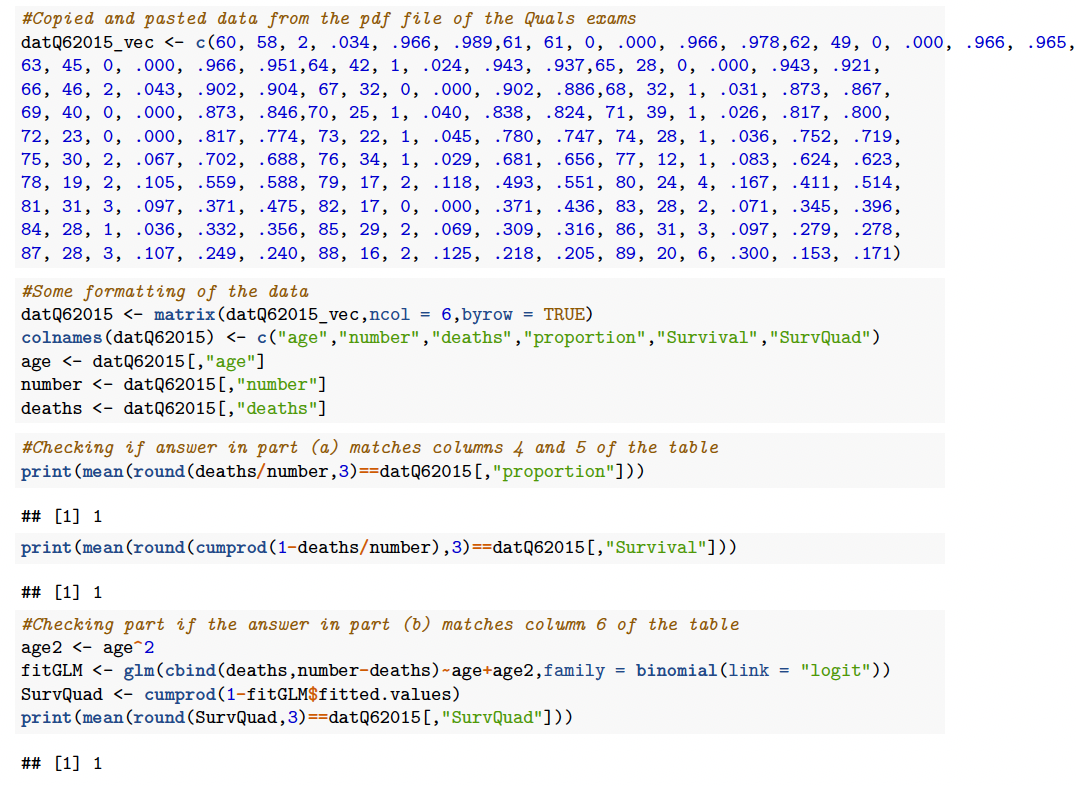
\includegraphics[width = \textwidth]{Q62015SanityCheck.png}



% \newpage
% \section{Applied 2016: Solution \footnote{Gene Katsevich, Kenneth Tay, Stephen Bates, Nikos Ignatiadis, Isaac Gibbs, Dan Kluger and M.H.}}

\subsection*{Problem 1: Quadratic discriminant analysis and EM}
Key ideas/tools:
\begin{itemize}
\item LDA and QDA as Gaussian mixture models
\item using EM for semi-supervised learning.
\end{itemize}


Let $y = 1$ denote ``otic" cells and $y = 0$ denote non-otic cells.

\begin{itemize}
\item[(a)] From the left plot, we see that the two Gaussian distributions have different means and covariance matrices. Hence, we can posit the following generative model:
	\begin{equation}
	\begin{split}
	&y_i \simiid \text{Ber}(\pi); \\
	&x_i|y_i=k \sim \mathcal N(\mu_k, \Sigma_k), \quad k = 0, 1. 
	\end{split}
	\end{equation}
	To fit these parameters, we can use maximum likelihood, for $k=0,1$,
	\begin{align}
	\hat \pi &= \frac{1}{n}\sum_{i = 1}^n y_i,\nonumber  \\
	 \hat \mu_k &= \frac{\sum_{i = 1}^n x_i I(y_i = k)}{\sum_{i = 1}^n I(y_i = k)},\nonumber  \\
	  \hat \Sigma_k &= \frac{\sum_{i = 1}^n (x_i-\hat \mu_k)(x_i - \hat \mu_k)^\top  I(y_i = k)}{\sum_{i = 1}^n I(y_i = k)}.
	\label{parameter_estimates}
	\end{align}
	Based on these fitted parameters, we can classify a point $x$ as otic if
	\begin{equation}
	\log \frac{\hat{\mathbb P}[y = 1|x]}{\hat{\mathbb P}[y = 0|x]} > 0,
	\label{decision}
	\end{equation}
	where $\hat{\mathbb{P}}$ is the probability distribution under the parameters $\hat{\pi}, \hat{\mu}_k$ and $\hat{\Sigma}_k$. This is quadratic discriminant analysis (QDA).
\item[(b)]  We have by Bayes' rule
	\begin{align}
	\log \frac{\mathbb P[y = 1|x]}{\mathbb P[y = 0|x]} &= \log\left(\frac{\pi}{1-\pi}\frac{\phi_{\mu_1, \Sigma_1}(x)}{\phi_{\mu_0, \Sigma_0}(x)}\right) \nonumber \\
	&= \log\left(\frac{\pi}{1 - \pi}\right) -\frac12 \log |\Sigma_1| - \frac{1}{2}(x - \mu_1)^\top  \Sigma_1^{-1}(x - \mu_1) \nonumber \\ &\qquad+ \frac12 \log |\Sigma_0| + \frac{1}{2}(x - \mu_0)^\top  \Sigma_0^{-1}(x - \mu_0). \label{log_odds}
	\end{align}
This quantity is a quadratic form in $x$, so we get a quadratic decision boundary. 

\item[(c)] I would take the parameter estimates from (\ref{parameter_estimates}) and plug them into the log-odds expression (\ref{log_odds}) together with the $x$ value of the new data point. Having calculated this log odds, I would classify the point based on (\ref{decision}).

\item[(d)] Intuitively, the unlabeled data carries information about $\mu_k$ and $\Sigma_k$. However, we cannot directly use these unlabeled data points without assigning them to classes. To address this problem, we can treat these unknown class labels as missing data, and estimate all the parameters with maximum likelihood estimation by using the EM algorithm. In the E step, we need to calculate the probability 
	\begin{equation}
	\mathbb P[z = 1|x, \pi^{(t)}, \mu_k^{(t)}, \Sigma_{k}^{(t)}].
	\end{equation}
	This is a calculation similar to (\ref{log_odds}). In the M step, we would plug these ``soft assignments" to calculate the expected complete-data likelihood and maximize with respect to the parameters. One way of initializing the EM algorithm is with the parameter estimates obtained from just the labeled data. 
	
	
	While the problem states ``briefly sketch how" and simply mentioning the above could suffice, if there is time on the exam it is worth sketching out in more detail how you would implement the EM algorithm. Let $N_l$, denote the number of labeled samples and $N_u$ denote the number of unlabeled samples $y_1,\dots, y_{N_l}$ are observed indicators of whether each labeled cell is otic and let $Z_{N_l+i}$ for $1 \le i \le N_u$ be the unobserved latent variable indicating whether or not the cell is otic. Note that our model for the data is,
\begin{align*}
y_i&\simiid \text{Ber}(\pi), \\
Z_i &\simiid  \text{Ber}(\pi),\\
 x_i|y_i=k &\sim \mathcal N(\mu_k, \Sigma_k), \\ 
 x_i|Z_i=k &\sim \mathcal N(\mu_k, \Sigma_k)
\end{align*}
	Letting $\theta= (\pi, \mu_0,\Sigma_0,\mu_1,\Sigma_1)$ denote the parameter of the model, and observe that the log-likelihood is given by 
$$\begin{aligned}
&\ell(\theta;X,Y) \\
& =\sum_{i=1}^{N_l} y_i \Big( \log(\pi)+ \log \big( \phi_{\mu_1, \Sigma_1}(x_i) \big) \Big)+(1-y_i) \Big( \log(1- \pi) +\log \big( \phi_{\mu_0, \Sigma_0}(x_i) \big) \Big) \\
& +\sum_{i=N_l+1}^{N_l+N_u}   \log \big( \pi \phi_{\mu_1, \Sigma_1}(x_i)  + (1-\pi) \phi_{\mu_0, \Sigma_0}(x_i) \big)
\end{aligned}$$

We seek to find the $\hat{\theta}$ maximizing the above expression. This can be done by using the EM algorithm, by noting that the complete log likelihood is given by 

$$\begin{aligned}
&\ell_c(\theta;X,Y,Z)\\
 & =\sum_{i=1}^{N_l} y_i \Big( \log(\pi)+  \log \big( \phi_{\mu_1, \Sigma_1}(x_i) \big) \Big)+(1-y_i) \Big( \log(1- \pi) + \log \big( \phi_{\mu_0, \Sigma_0}(x_i) \big) \Big) \\
& +\sum_{i=N_l+1}^{N_l+N_u}  Z_i \Big( \log(\pi)+ \log \big( \phi_{\mu_1, \Sigma_1}(x_i) \big) \Big)+ (1-Z_i) \Big( \log(1-\pi) + \log \big( \phi_{\mu_0, \Sigma_0}(x_i) \big) \Big).
\end{aligned}$$

To implement the E-step for each $\hat{\theta},i$ define $\gamma_{\hat{\theta},i} = y_i$ if $i \in \{1,\dots,N_l \}$ and define 
\begin{align*}
	\gamma_{\hat{\theta},i} &:=\mathbb{E}_{\hat{\theta}} [Z_i |X,Y]\\
	& =\mathbb{P}_{\hat{\theta}} [Z_i=1|x_i] \\
	&= \frac{\hat{\pi} \phi_{\hat{\mu}_1, \hat{\Sigma}_1}(x_i) }{\hat{\pi} \phi_{\hat{\mu}_1, \hat{\Sigma}_1}(x_i)+(1-\hat{\pi}) \phi_{\hat{\mu}_0, \hat{\Sigma}_0}(x_i)}
\end{align*} 
For $N_l < i \leq N_l+N_u,$. The expected complete log-likelihood conditional on the observed data is given by
\begin{align}\label{eq:EStep}
&\mathbb{E}_{\hat{\theta}} \big[l_c(\theta;X,Y,Z) \big| X,Y \big] \nonumber \\
&= \sum_{i=1}^{N} \gamma_{\hat{\theta},i} \Big( \log(\pi) + \log \big( \phi_{\mu_1, \Sigma_1}(x_i) \big) \Big) + \Big( \log(1-\pi)  +   (1-\gamma_{\hat{\theta},i}) \log \big( \phi_{\mu_0, \Sigma_0}(x_i) \big) \Big),
\end{align}
where $N =N_l+N_u$.

To implement the M-step, note that the above objective is separable in $\pi$, $(\mu_0,\Sigma_0)$ and $(\mu_1,\Sigma_1)$. By taking the derivative with respect to $\pi$ setting to $0$ and by taking the gradients with respect to $(\mu_k,\Sigma_k)$ for $k=0,1$ and setting to zero,

$$\pi^{(t+1)} = \frac{1}{N} \sum_{i=1}^N \gamma_{\theta^{(t)},i}, \quad \mu_1^{(t+1)} = \frac{ \sum_{i=1}^N \gamma_{\theta^{(t)},i} x_i}{\sum_{i=1}^N  \gamma_{\theta^{(t)},i}  } , \quad \mu_0^{(t+1)} = \frac{\sum_{i=1}^N (1- \gamma_{\theta^{(t)},i} ) x_i}{\sum_{i=1}^N (1- \gamma_{\theta^{(t)},i} ) },$$
and 
\begin{align*} 
	\Sigma_1^{(t+1)}&= \frac{\sum_{i=1}^N \gamma_{\theta^{(t)},i} (x_i - \mu_1^{(t+1)})(x_i -\mu_1^{(t+1)})^\top  }{\sum_{i=1}^N  \gamma_{\theta^{(t)},i}  },\\
	  \Sigma_0^{(t+1)} &= \frac{\sum_{i=1}^N (1-\gamma_{\theta^{(t)},i}  )(x_i - \mu_0^{(t+1)})(x_i -\mu_0^{(t+1)})^\top }{\sum_{i=1}^N (1- \gamma_{\theta^{(t)},i} ) }.
\end{align*}
Note that solving for $\Sigma_k^{(t+1)}$ in the M-step is a bit tricky and can be done using formulas (57) and (61) in the Matrix cookbook. To find the maximum likelihood you alternate between the E-step and M-step updating $\hat{\theta} =\theta^{(t+1)}$. As mentioned earlier one good way to initialize the EM algorithm here is to use the estimates from part (a).
\end{itemize}


% Problem 2
\subsection*{Problem 2: Three angles and measurement error}

Key ideas/tools:
\begin{itemize}
\item writing down a model
\item maximum likelihood estimation
\end{itemize}


We find that the angles do not add up exactly to 180$^\circ$. The problem is that these angles contain measurement error.

In order to estimate the true angles, we must postulate a probability model for the measurement error. If the measurements are $y_1, y_2, y_3$ and the true angles are $\theta_1, \theta_2, \theta_3$, then the simplest model for measurement error is
\begin{equation}
y_i = \theta_i + \eps_i, \quad \eps_{i} \overset{\text{i.i.d.}}\sim \mathcal N(0, \sigma^2).
\end{equation}
Assuming a constant error variance would be problematic if the angles were very different in size (e.g. if one of the angles was $1^\circ$), but in our case it seems reasonable. We have the additional constraint that $\theta_1 + \theta_2 + \theta_3 = 180$, so we can parameterize the problem using $(\theta_1, \theta_2)$ only. Hence, we can estimate these two parameters from the following linear regression:
\begin{equation}
\left( \begin{array}{c}
y_1 \\
y_2 \\
y_3 - 180 \end{array} \right)= \left( \begin{array}{cc}
1 & 0 \\
0 & 1\\
-1 & -1 \end{array} \right)\left( \begin{array}{c}
\theta_1 \\
\theta_2 \end{array} \right) + \left( \begin{array}{c}
\eps_1 \\
\eps_2 \\
\eps_3 \end{array} \right). 
\end{equation}
Then, $(\hat \theta_1, \hat \theta_2, 180 - \hat \theta_1 - \hat \theta_2)$ would be our best guess for the true angles (these should also satisfy the constraints of positive angles, otherwise we could incorporate the constraints into the least squares optimization). The OLS estimate ends up being 
\begin{align*}
	\begin{bmatrix}
		\hat{Y}_1 \\ \hat{Y}_2 \\ \hat{Y}_3
	\end{bmatrix} &= \begin{bmatrix}
		\frac{2}{3}Y_1 - \frac{1}{3}(Y_2+Y_3) + 60^\circ\\
		\frac{2}{3}Y_2 - \frac{1}{3}(Y_1+Y_3) + 60^\circ\\
		\frac{2}{3}Y_3 - \frac{1}{3}(Y_1+Y_2) + 60^\circ
	\end{bmatrix}
\end{align*}


% Problem 3
\subsection*{Problem 3: A missing species problem}
Key ideas/tools:
\begin{itemize}
\item mixture models
\item Empirical Bayes
\end{itemize}

\paragraph{Context:} \citet{efron2016empirical} proposes empirical Bayes estimation in which the prior is specified as a flexible exponential family. Estimation can proceed parametrically by maximum likelihood. I think the question is not worded very clearly and may be interpreted in multiple ways depending on how you interpret the description of the distribution of $X_i$. Below we just present one interpretation.

\begin{itemize}
\item[(a)] We have
	\begin{equation}
	\begin{split}
	f_k = \mathbb P[X_i = k] &= \sum_{j = 1}^m \mathbb P[X_i = k, \Theta_i = \theta_{(j)}] \\
	&= \sum_{j = 1}^m \mathbb P[\Theta_i = \theta_{(j)}]\mathbb P[X_i = k|\Theta_i = \theta_{(j)}] \\
	&= \sum_{j = 1}^m g_j e^{-\theta_{(j)}}\frac{\theta_{(j)}^k}{k!}.
	\end{split}
	\end{equation}
	Hence, 
	\begin{equation}
	p_{kj} =  e^{-\theta_{(j)}}\frac{\theta_{(j)}^k}{k!}.
	\end{equation}

\item[(b)] Let $P_k = (p_{k1} , p_{k2} , \dots, p_{km})$. Note that the likelihood for one observation of a species trapped $k$ times
	\begin{equation*}
	\tilde{f}_k(\alpha) = \mathbb P[X_i = k|X_i > 0] = \frac{f_k}{1 - f_0} = \frac{P_k^\top  \mathbf{g}(\alpha)}{1 - P_0^\top  \mathbf{g}(\alpha)}.
	\end{equation*}
	
	Therefore the log-likelihood for our count data is given by
	\begin{align*}
	\ell(\alpha) &= \sum_{k=1}^{100} y_k \log \big(  \tilde{f}_k(\alpha) \big)\\
	&=  \sum_{k=1}^{100} y_k  \log \big( P_k^\top  \mathbf{g}(\alpha) \big) -  \log \big( 1-P_0^\top  \mathbf{g}(\alpha) \big)  \sum_{k=1}^{100} y_k
	\end{align*}
	
	We can then fit $\hat \alpha$ by maximum likelihood:
	\begin{equation*}
	\hat \alpha = \underset{\alpha}{\arg \max} \ \Bigg( \sum_{k=1}^{100} y_k  \log \big( P_k^\top  \mathbf{g}(\alpha) \big) - \log \big( 1-P_0^\top  \mathbf{g}(\alpha) \big)  \sum_{k=1}^{100} y_k \Bigg)
	\end{equation*}
	 \citet{efron2016empirical} actually uses a direct second order numerical optimization routine and explicitly calculates gradients (the Score) and Hessians of $\ell$ w.r.t. $\alpha$. Another natural way of optimizing this problem is with the EM algorithm. For the EM based approach, let $X_1,\dots,X_n$ be the number of times each observed species is trapped and let $\Theta_1,\dots,\Theta_n$ be the unobserved latent variable for each species. The complete log-likelihood, is given by $$\ell_c( \alpha; X , \Theta ) = \sum_{i=1}^n \sum_{k=1}^{100} \sum_{j=1}^m I \{ \Theta_i = \theta_{(j)}, X_i=k \} \Big( \log \big( \mathbf{g} (\alpha)_j \big) + \log \big( \frac{p_{kj}}{1-p_{0j}}\big) \Big).$$
	
	To compute the E-step note that $$\gamma_{\tilde{\alpha},k,j} \equiv P_{\tilde{\alpha}} ( \Theta_i = \theta_{(j)} |X_i =k ) =\frac{\mathbf{g} (\alpha)_j p_{kj}/(1-p_{0j})}{ \sum_{j'=1}^m \mathbf{g} (\alpha)_{j'} p_{kj'}/(1-p_{0j'}) },$$ so the expected complete log likelihood (up to an additive constant which doesn't depend on $\alpha$) is given by $$\mathbb{E}_{\tilde{\alpha}}[\ell_c( \alpha; X , \Theta )| X] = \sum_{k=1}^{100} \sum_{j=1}^m y_k \gamma_{\tilde{\alpha},k,j} \log \big( \mathbf{g} (\alpha)_j \big).$$ Depending on the function form of $\mathbf{g}$ the M-step could require using Lagrange Multipliers.

\item[(c)]  If we had access to the full data (i.e., we also observed $y_0 = \#\{i: X_i = 0\}$), the log-likelihood is given by 

$$\ell(\mathbf{h}) = \sum_{k = 0}^{100} y_k \log \Big( P_k^\top  \mathbf{h} \Big),$$ where $P_k = (p_{k1} , p_{k2} , \dots, p_{km})$ for $k=0,\dots,100$ are the fixed vectors defined in part (b). Observe that the log-likelihood is concave in $\mathbf{h}$, because $\log$ is concave, the $\log$ composed with a linear function in $\mathbf{h}$ is also concave and hence each $ \log \Big( P_k^\top  \mathbf{h} \Big)$ term is concave in $\mathbf{h}$. Further all $y_k \geq 0$, so $\ell(\mathbf{h})$ is a positive weighted sum of concave functions in $\mathbf{h}$ and hence $\ell(\mathbf{h})$ is concave.

We can thus estimate $\mathbf{h}$ by minimizing the negative log likelihood $-\ell(\mathbf{h})$ subject to the constraint that $h_i \geq 0$ and $\sum_{i=1}^m h_i =1$. In particular we can find the $\mathbf{h}$ that solves the following convex optimization problem in $\mathbf{h}$:

 $$\begin{aligned}
 \text{minimize} & \ \ \ \ -\sum_{k = 0}^{100} y_k \log \Big( P_k^\top  \mathbf{h} \Big)
 \\ \text{subject to} & \ \ \ \ h_i \geq 0, \ \ \ i=1,...,m 
 \\ & \ \ \ \ \mathbf{1}^\top  \mathbf{h} =1.
 \end{aligned}$$


%\begin{equation*}
%	\hat \alpha = \underset{\alpha}{\arg \max} \ \sum_{k = 0}^{100} y_k \log \Big( P_k^\top  \mathbf{h} (\alpha ) \Big).
%	\end{equation*}
\end{itemize}

% Problem 4
\subsection*{Problem 4: Separation in logistic regression without intercept}

Key ideas/tools:
\begin{itemize}
\item manipulating the logistic regression likelihood
\end{itemize}


We have pairs $(x_i, y_i)$, $i = 1, \dots, n$, that we model as
\begin{equation}
y_i \overset{\text{ind}}\sim \text{Ber}(p_i), \quad \text{logit}(p_i) = \beta x_i.
\end{equation}
Because $y_i = 1$ for all $i$, we get a log-likelihood of
\begin{equation}
\ell(\beta) = \log \prod_{i=1}^n p_i = \sum_{i=1}^n \log \Big(  \frac{e^{\beta x_i}}{1+e^{\beta x_i}}\Big)= \beta \sum_{i = 1}^n x_i - \sum_{i = 1}^n \log(1 + e^{\beta x_i}).
\label{logistic_likelihood}
\end{equation}

We know that usually in logistic regression, we have problems when the data are perfectly separated. However, the situation is a bit different here because the regression has no intercept term. With this constraint, the function $\mathbb P[y = 1|x]$ must pass through the point (0, 1/2), as in Figure \ref{fig:logistic}. By looking at this figure, it is clear we can fit the data increasingly well by sending $\beta \rightarrow \infty$ if $x_i \geq 0$ for all $i$. By flipping the sign of $\beta$, we can also fit the data increasingly well by sending $\beta \rightarrow -\infty$ if $x_i \leq 0$ for all $i$. In these cases, we do not get a finite MLE.

On the other hand, if there is at least one $x_i > 0$ and at least one $x_i < 0$, then $|\beta| \rightarrow \infty$ would lead to a log-likelihood tending to negative infinity. Since the log-likelihood is concave in $\beta$ (we can check that $\ddot{\ell}(\beta) <0$), this means that it has a unique finite maximizer.
\begin{figure}
	\centering
	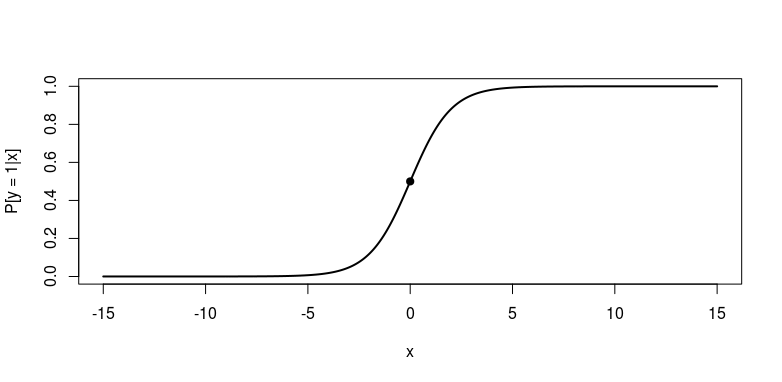
\includegraphics[width = 0.9\textwidth]{logistic_function.png}
	\caption{Logistic regression through the origin; $\beta = 1$.}
	\label{fig:logistic}
\end{figure}


% Problem 5
\subsection*{Problem 5: ANOVA -- with interactions without}

Key ideas/tools:
\begin{itemize}
\item calculations with the linear model
\end{itemize}

Here we present two solutions. The first uses vectorized notation, the second works with the coordinates. 
 
\subsubsection*{Vectorized solutions}

Let $\ones_I$ and $\ones_J$ represent the vectors of all $1$'s in dimensions $I$ and $J$ respectively. The ``outer product'' $\ones_I\ones_J^\top $ is a matrix in $\reals^{I \times J}$ of all $1$'s. We will think of $Y = (Y_{ij})$ as an element of $\reals^{I \times J}$. The given model can be written as 
\[Y = \mu \ones_I \ones_J^\top  + \alpha \ones_J^\top  + \ones_J \beta^\top  + \gamma + e, \]
where $e \in \reals^{I \times J}$ has i.i.d. entries with mean 0 and variance $\sigma^2$. The constraints on $\alpha,\beta$ and $\gamma$ can be written in vector notation,
\begin{align*}
	\alpha^\top  \ones_I&=0,\\
	\beta^\top  \ones_J&=0,\\
	\gamma \ones_J &= 0,\\
	\gamma^\top  \ones_I &=0.
\end{align*}
In particular, $\gamma$ is orthogonal to the space of main affects 
\begin{equation}\label{eq:subspace}U = \{\mu\ones_I\ones_J^\top  + \alpha \ones_J^\top  +\ones_I\beta^\top  \} \subseteq \reals^{I \times J}. \end{equation}
With this notation we will continue the question.
\begin{enumerate}
	\item[(a)] In this model, the OLS estimate of $\mu$ is the grand mean,
	\[\hat{\mu}=\bar{Y}_{+,+}=\frac{1}{IJ}\sum_{i=1}^I\sum_{j=1}^J Y_{i,j} = \frac{1}{IJ} \ones_I^\top  Y \ones_J. \]
	The OLS estimate of $\alpha$ is
	\[\hat{\alpha}_i = \bar{Y}_{i,+}-\bar{Y}_{+,+},  \]
	where $\bar{Y}_{i,+}$ is the group mean for level $i$. That is, 
	\[\bar{Y}_{i,+} = \frac{1}{J}\sum_{j=1}^J Y_{i,j}=\frac{1}{J}\left(Y\ones_J\right)_i .\] 
	We can calculate the expectation of $\bar{Y}_{i,+}$
	\begin{align*}
		\mathbb{E}[\bar{Y}_{i,+}]&=\frac{1}{J}\sum_{j=1}^J \bbE[Y_{i,j}]\\
		&=\frac{1}{J}\sum_{j=1}^J \mu+\alpha_i+\beta_j +\gamma_{ij} + \bbE[e_{ij}]\\
		&=\mu+\alpha_i,
	\end{align*}
	since $\beta_j^\top  \ones_J = 0$, $\gamma \ones_J=0$ and $\bbE[e_{ij}]=0$. By a similar calculation, the expectation of $\bar{Y}_{+,+}$ is $\mu$ and thus,
	\[\bbE[\hat{\alpha}_i] = \bbE[Y_{i,+}] - \bbE[\bar{Y}_{+,+}] = \mu +\alpha_i - \mu = \alpha_i. \]
	Thus,
	\[\bbE[\hat{\alpha}_i-\hat{\alpha}_{i'}] = \alpha_i-\alpha_{i'}, \]
	so the OLS estimate for $\alpha_i-\alpha_{i'}$ is unbiased.
	\item[(b)] Let $\hat{Y} \in \reals^{I\times J}$ be the fitted values in the main affects model. The main effects model has $I+J-1$ degrees of freedom (there are $I+J+1$ parameters and $2$ constraints). The usual estimate $\hat{\sigma}^2$ is thus
	\[\hat{\sigma}^2 = \frac{1}{IJ-(I+J-1)}\Vert Y - \hat{Y} \Vert_F^2 = \frac{1}{(I-1)(J-1)}\Vert Y - \hat{Y}_F^2 \]
	where $\Vert \cdot \Vert_F$ is the Frobenius norm on $\reals^{I \times J}$. Let $H$ be the projection onto the subspace $U$ from \eqref{eq:subspace}. We thus have,
	\begin{align*}
		Y-\hat{Y}&=(I-H)Y\\
		&=(I-H)(\mu\ones_I\ones^\top _J + \alpha\ones_J^\top  + \ones_I\beta^\top  +\gamma + e)\\
		&=\gamma + (I-H)e.
	\end{align*}
	The last line holds because by definition the main effects $\mu\ones_I\ones^\top _J + \alpha\ones_J^\top  + \ones_I\beta^\top $ are in $U$ and because $\gamma$ is orthogonal to $U$. Note that the rank of $(I-H)$ is exactly $IJ-(I+J+1)=(I-1)(J-1)$ and thus,
	\begin{align*}
		\bbE[\hat{\sigma}^2]&=\frac{1}{(I-1)(J-1)}\bbE[\Vert \gamma + (I-H)e\Vert_F^2]\\
		&=\frac{1}{(I-1)(J-1)}\bbE\left[\Vert \gamma \Vert_F^2 + 2\gamma^\top  (I-H)e + \Vert (I-H)e\Vert_F^2 \right] \\
		&=\frac{1}{(I-1)(J-1)}\left(\Vert \gamma \Vert_F^2 + (I-1)(J-1)\sigma^2\right)\\
		&=\sigma^2 + \frac{\Vert \gamma \Vert_F^2}{(I-1)(J-1)}.
	\end{align*}
	That is $\hat{\sigma}^2$ is biased upwards by,
	\[\frac{1}{(I-1)(J-1)} \Vert \gamma \Vert_F^2 = \frac{1}{(I-1)(J-1)}\sum_{i=1}^I\sum_{j=1}^J \gamma_{ij}^2 \ge 0. \]
	If we make the additional assumption that $e_{ij} \simiid \mathcal{N}(0,\sigma^2)$, then we can identify the distribution of $\hat{\sigma}^2$. By the above calculations we have 
	\[Y-\hat{Y} \sim \mathcal{N}_{I \times J}(\gamma, \sigma^2(I-H)), \]
	thus 
	\[\hat{\sigma}^2 = \frac{1}{(I-1)(J-1)}\Vert Y-\hat{Y}\Vert_F^2 \sim \frac{\sigma^2}{(I-1)(J-1)} \chi^2_{(I-1)(J-1)}(\Vert \gamma \Vert_F^2).\] 
	That is $\hat{\sigma}^2$ is a scaled non-central $\chi^2$ distribution.
	\item[(c)] As seen above
	\[\hat{\alpha}_2 - \hat{\alpha}_1 = \bar{Y}_{2,+} - \bar{Y}_{1,+} = \frac{1}{2}\left(Y_{2,1}+Y_{2,2}\right) - \frac{1}{2}\left(Y_{1,1}+Y_{1,2}\right), \]
	is unbiased of $\alpha_2 - \alpha_1$. Thus, we can $\alpha_1 - \alpha_2$ is identifiable. 
\end{enumerate}


\subsubsection*{Coordinate solution}

\begin{itemize}
\item[(a)] In fact, the usual least squares estimates of $\alpha_i$ are unbiased. Indeed,
		\begin{equation}
		\begin{split}
		\mathbb E[\hat \alpha_i] &= \mathbb E[\overline Y_{i+} - \overline Y_{+ +}] \\
		&= \mathbb E\left[\frac{1}{J}\sum_{j = 1}^J (\mu + \alpha_i + \beta_j + \gamma_{ij} + e_{ij}) - \frac{1}{IJ}\sum_{i = 1}^I \sum_{j = 1}^{J}(\mu + \alpha_i + \beta_j + \gamma_{ij} + e_{ij}) \right] \\
		&= \mu + \alpha_i - \mu \\
		&= \alpha_i
		\end{split}
		\end{equation}

Thus, the usual least squares estimates of $\alpha_i - \alpha_{i'}$ will also be unbiased.

\item[(b)] Note that 
\begin{align*}
\hat{\mu} &= \frac{1}{IJ} \sum_{i,j} Y_{ij} = \frac{1}{IJ}\sum_{i,j} (\mu +  e_{ij}) = \mu + \overline e_{+ +}, \\ 
\hat{\alpha_i} &= \frac{1}{J} \sum_j Y_{ij} - \frac{1}{IJ} \sum_{i,j} Y_{ij} = \alpha_i + \overline e_{i +} - \overline e_{+ +}, \\
\hat{\beta_j} &= \frac{1}{I} \sum_i Y_{ij} - \frac{1}{IJ} \sum_{i,j} Y_{ij} = \beta_j + \overline e_{+ j} - \overline e_{+ +}.
\end{align*}

Thus, we have
		\begin{equation*}
		\begin{split}
		\mathbb E[\hat \sigma^2] &= \mathbb E\left[\frac{1}{(I-1)(J-1)}\sum_{i = 1}^I \sum_{j = 1}^J (Y_{ij} - \hat \mu - \hat \alpha_i - \hat \beta_j)^2\right] \\
		&= \mathbb E\left[\frac{1}{(I-1)(J-1)}\sum_{i = 1}^I \sum_{j = 1}^J (\gamma_{ij} + e_{ij} - \overline e_{i+} - \overline e_{+ j} + \overline e_{+ +})^2\right] \\
		&= \frac{1}{(I-1)(J-1)}\sum_{i = 1}^I \sum_{j = 1}^J \mathbb E\left[(\gamma_{ij} + e_{ij} - \overline e_{i+} - \overline e_{+ j} + \overline e_{+ +})^2\right] \\
		&= \mathbb E\left[\frac{1}{(I-1)(J-1)}\sum_{i = 1}^I \sum_{j = 1}^J (e_{ij} - \overline e_{i+} - \overline e_{+ j} + \overline e_{+ +})^2\right] + \frac{1}{(I-1)(J-1)}\sum_{i = 1}^I \sum_{j = 1}^J \gamma_{ij}^2 \\
		&= \sigma^2 + \frac{1}{(I-1)(J-1)}\sum_{i = 1}^I \sum_{j = 1}^J \gamma_{ij}^2.
		\end{split}
		\end{equation*}
		The last equality holds because the quantity in brackets in the penultimate line is the unbiased estimate for $\sigma^2$ in the no-interactions model. Hence, we find that $\hat \sigma^2$ is biased upwards for $\sigma^2$. This will have the effect of deflating the significance of $F$ tests for $\alpha_1 = \cdots = \alpha_I$ and $\beta_1= \cdots = \beta_J$. 
		
		Another way to see that the last line above holds is to use linearity of expectation and to note that since $e_{ij} \stackrel{\text{IID}}{\sim} N(0,\sigma^2)$, then for each $i,j$, $$\begin{bmatrix} e_{ij} \\  \overline e_{i +} \\ \overline e_{+ j} \\  \overline e_{+ +}  \end{bmatrix} \sim \mathcal{N} \Bigg( \begin{bmatrix} 0 \\  0 \\ 0 \\  0  \end{bmatrix}, \sigma^2 \begin{bmatrix} 1  & \frac{1}{J} & \frac{1}{I} & \frac{1}{IJ} \\ \frac{1}{J} & \frac{1}{J} & \frac{1}{IJ}  &  \frac{1}{IJ} \\ \frac{1}{I} & \frac{1}{IJ} & \frac{1}{I} &  \frac{1}{IJ} \\ \frac{1}{IJ} &  \frac{1}{IJ} &  \frac{1}{IJ} & \frac{1}{IJ}  \end{bmatrix}  \Bigg)$$ and hence letting $v=(1,-1,-1,1)$,  $$e_{ij} - \overline e_{i+} - \overline e_{+ j} + \overline e_{+ +} \sim \mathcal{N} \Bigg(0, \sigma^2 v^\top   \begin{bmatrix} 1  & \frac{1}{J} & \frac{1}{I} & \frac{1}{IJ} \\ \frac{1}{J} & \frac{1}{J} & \frac{1}{IJ}  &  \frac{1}{IJ} \\ \frac{1}{I} & \frac{1}{IJ} & \frac{1}{I} &  \frac{1}{IJ} \\ \frac{1}{IJ} &  \frac{1}{IJ} &  \frac{1}{IJ} & \frac{1}{IJ}  \end{bmatrix} v \Bigg) = \mathcal{N}\big( 0, \sigma^2 (1 -\frac{1}{J} -\frac{1}{I} + \frac{1}{IJ} ) \big),$$ so indeed $$\frac{1}{(I-1)(J-1)}\sum_{i = 1}^I \sum_{j = 1}^J  \mathbb{E} \left[ (e_{ij} - \overline e_{i+} - \overline e_{+ j} + \overline e_{+ +})^2\right] =\sigma^2.$$

\item[(c)] A direct way of checking identifiability is to note that

$$ \EE{ \frac{Y_{11}  + Y_{12}}{2} - \frac{Y_{21}  + Y_{22}}{2}} = \alpha_1 - \alpha_2. $$

\end{itemize}



% Problem 6
\subsection*{Problem 6: Testing linearity with replicates}
Key ideas/tools:
\begin{itemize}
\item F-test
\item residual bootstrap
\end{itemize}
\begin{itemize}
\item[(a)] Given i.i.d. normal errors, we can use the $F$ test to compare 
	\begin{equation}
	H_0: y_{ij} = \beta_0 + \beta_1 x_i + e_{ij} \quad \text{vs.} \quad H_1: y_{ij} = \sum_{i' = 1}^k \beta_{i'} I(x_i = x_{i'}) + e_{ij}.
	\end{equation}
	Here, $H_0$ represents the linear model and $H_1$ represents the saturated model.
	The resulting F statistic is
	\begin{equation}
	F = \frac{\frac{1}{k - 2}\sum_{i, j}(\overline y_{i\cdot} - \hat \beta_0 - \hat \beta_1 x_i)^2}{\frac{1}{km-k}\sum_{i, j}(y_{ij} - \overline y_{i\cdot})^2}.
	\label{F}
	\end{equation}
	This is the ratio of the ``lack of fit sum of squares" to the ``pure error sum of squares," and has a null distribution of $F_{k-2, km-k}$.

\item[(b)] The main idea here is to describe some sort of bootstrap test. However, there are many possible ways to set this up. Here are the solutions that have acculated over the years.

\textbf{Solution 1:} Suppose that $y_{ij} = m(x_i) + e_{ij}$, where $e_{ij} \overset{\text{i.i.d.}}\sim F$ for some unknown error distribution $F$ with mean $0$.  A reasonable approach here is to bootstrap residuals. In particular let $\hat{e}_{ij} =  y_{ij} - \hat{\beta}_0 - \hat{\beta}_1x_i$. Then, we can generate bootstrap datasets by setting
\[
	y_{ij}^* = \hat \beta_0 + \hat \beta_1 x_{i} + \hat{e}_{ij}^*
\]
where $\hat{e}_{ij}^*$ are sampled with replacement from the set $\{\hat e_{ij}\}$. We can then recalculate the $F$ statistic (\ref{F}) for each bootstrapped data set and thereby generate its null distribution.\\

I think it is instructive to also consider the solution of a previous coach who suggested to use the same procedure, but with $\hat{e}_{ij}  = y_{ij} - \bar{y}_{i\cdot}$. Note that in this case $\hat{e}_{ij} = e_{ij} - \bar{e}_{i \cdot}$. If $m$ is small the empirical distribution of $\hat{e}_{ij}$ may not be very close to $F$ and thus we probably should not expect this procedure to work. On the other hand, if $m$ is large this is likely also valid.\\  
    
If we think that the error distribution changes with $x$ (e.g. if there is heteroskedasticity), then we can also resample the residuals separately for each $x$. However, this will also probably only work when $m$ is large.

A previous coach also suggested that when $m$ is large, we may still trust using the F-test from part (a), if $m$ is large enough for the Central Limit Theorem has kicked in. Typically we expect the Central Limit Theorem to kick in whenever $n \gg p$ or equivalently in this case when $m \gg 1$. However, while I see how the Central Limit Theorem can kick in for the numerator of the $F$-statistic as $m \to \infty$, I don't quite see how in the limit as $m \to \infty$ the central limit theorem would kick in for the denominator and make it approximately $\chi_{km-k}^2$.

\textbf{Alternative solutions when $m$ is fixed $k \to \infty$:} An alternative solution is to explicitly evaluate the limiting distribution of the F-statistics. Let $X \in \mmr^{m k \times 2}$ be the design matrix with rows $X_1,\dots,X_{m k }$. Write
\begin{align*}
F = \frac{km-k}{k-2} \left( \frac{y^\top (I-X(X^\top X)^{-1}X^\top )y}{\sum_{i,j}(e_{ij} - \bar{e}_{i \cdot})^2} - 1 \right) = \frac{km-k}{k-2} \left( \frac{e^\top (I-X(X^\top X)^{-1}X^\top )e}{\sum_{i,j}(e_{ij} - \bar{e}_{i \cdot})^2} - 1 \right) 
\end{align*}
Without loss of generality assume that the second column of $X$ is centred and both columns are scaled so that $X^\top X = I$. Then,
\begin{align*}
F & =  \frac{km-k}{k-2} \left( \frac{e^\top e - ||\sum_{i,j} x_i e_{ij}||^2   }{\sum_{i,j}(e_{ij} - \bar{e}_{i \cdot})^2} - 1 \right)\\
&  =  \frac{km-k}{k-2} \left(\frac{m\sum_{i} (\bar{e}_{i\cdot})^2  }{\sum_{i,j}e_{ij}^2 - (\bar{e}_{i \cdot})^2}  \right) - O_P(1/k)\\
& =  \frac{km-k}{k-2} \left(\frac{m^{-1}\sum_{i,j} e_{ij}^2  +  m^{-1}\sum_{i} \sum_{j \neq j'} e_{ij}e_{ij'}  }{(1-1/m)\sum_{i,j}e_{ij}^2 - (1/m) \sum_{j \neq j'} e_{ij} e_{ij'}  }  \right) - O_P(1/k)
\end{align*}
So, we find that 
\begin{align*}
\sqrt{k}\left(F - \frac{k}{k-2}\right) & = \sqrt{k} \frac{k}{k-2} \left(\frac{m^{-1}\sum_{i,j} e_{ij}^2  + m^{-1} \sum_{i} \sum_{j \neq j'} e_{ij}e_{ij'}  }{  m^{-1} \sum_{i,j}e_{ij}^2 - m^{-1}(m-1)^{-1} \sum_{j \neq j'} e_{ij} e_{ij'}  } - 1 \right) - O_P(1/k)\\
& = \sqrt{k} \frac{k}{k-2} \left(   \frac{  (m-1)^{-1} \sum_{i} \sum_{j \neq j'} e_{ij}e_{ij'} }{  m^{-1} \sum_{i,j}e_{ij}^2 - m^{-1}(m-1)^{-1} \sum_{j \neq j'} e_{ij} e_{ij'}  }    \right) - O_P(1/k)\\
& \stackrel{D}{\to} N(0, 2m(m-1))
\end{align*}
Note that the limiting distribution does not depend on the distribution of the errors and in particular the limiting distribution when $e_{ij} \sim N(0,\sigma^2)$ is the same as the limiting distribution in the case where $e_{ij} \sim F$ for $F$ an arbitrary distribution with a finite second moment. Thus, the F-test proposed in part a will be accurate without needing to assume normality. 



\item[(c)] If there had been no replication, then the denominator of the $F$ statistic would be zero, i.e. the $F$ test would not be valid. Hence, we need to make our saturated model a little less saturated. For example, if Engineer A sees a polynomial-looking relationship between $y$ and $x$, then one could do an $F$ test versus a larger model with some higher-order terms in $x$. Bootstrapping residuals could also work in this case. 

If we have densely spaced covariate values $x_i$, another approach we could take is to approximate the lack of fit $F$ test by simply grouping points with similar $x_i$. In general, this approach will underestimate the difference between $x_i^\top \beta$ and $m(x_i)$ and thus will produce a conservative test.

\item[(d)] We would question the independence of errors across $i$ if $i$ indexed space or time. We know that spatial and temporal data often exhibit local correlations in errors. We would question the independence of $e_{ij}$ across $j$ if there were systematic differences in the data collection process across $i$, e.g. if $i$ indexes days and a different person collected the data on each day. This would introduce positive correlations among $e_{ij}$ for each $i$, which would inflate our $F$ statistics by underestimating their denominators.

\end{itemize}

% \newpage 
% \section{Applied 2017: Solution \footnote{Kenneth Tay, Stephen Bates, Nikos Ignatiadis, Isaac Gibbs, D.K.}}

\subsection*{Problem 1: Bayesian Logistic Regression}
Key ideas/tools:
\begin{itemize}
\item setting up hierarchical models
\item the connection between the posterior mode and penalized estimation
\end{itemize}

\begin{enumerate}
\item[(a)] The model is (treating $x_{ij}$ as fixed)
\begin{equation}
\beta \mid \tau \sim \calN(0, \tau^2 I_p), \qquad y_{ij} \mid \beta \stackrel{ind}{\sim} \text{Ber}(p_{ij}), \text{ where } \text{logit}(p_{ij}) = x_{ij}^\top\beta.
\end{equation}

\item[(b)] In this set-up, we are assuming that $X$ is fixed. Then the posterior is \begin{align*}
p(\beta \mid y) &\propto p(\beta) p (y \mid \beta) \\ 
&\propto \exp \left( - \frac{1}{2\tau^2} \|\beta\|^2 \right) \cdot \prod_{i,j} \left[\left( \frac{\exp (x_{ij}^T \beta)}{1 + \exp (x_{ij}^T \beta)} \right)^{y_{ij}} \left( \frac{1}{1 + \exp (x_{ij}^T \beta)} \right)^{1 - y_{ij}}\right] \\ 
&= \exp \left( - \frac{1}{2\tau^2} \|\beta\|^2 \right) \cdot \prod_{i,j} \frac{\left[\exp (x_{ij}^T \beta) \right]^{y_{ij}}}{1 + \exp (x_{ij}^T \beta)}.
\end{align*}

Thus, the posterior distribution can be written as
\begin{equation}\label{eq:posteriorBasketball}
p(\beta \mid y) = \frac{\exp \left( - \frac{1}{2\tau^2} \|\beta\|^2 \right) \cdot \prod_{i,j} \frac{\left[\exp (x_{ij}^T \beta) \right]^{y_{ij}}}{1 + \exp (x_{ij}^T \beta)}}{\int_{\bbR^p} \exp \left( - \frac{1}{2\tau^2} \|\beta\|^2 \right) \cdot \prod_{i,j} \frac{\left[\exp (x_{ij}^T \beta) \right]^{y_{ij}}}{1 + \exp (x_{ij}^T \beta)} d \beta}.
\end{equation}

Computing the posterior mode of $\beta$ --also called the MAP (Maximum a-posteriori) estimator-- amounts to minimizing 
\begin{equation}
\label{eq:posterior_median}
- \log p(\beta \mid y) = \frac{1}{2\tau^2} \|\beta\|^2 - \sum_{i,j} \left[ y_{ij} x_{ij}^T \beta - \log (1 + \exp(x_{ij}^T \beta)) \right].
\end{equation}
Notice the posterior mode is exactly equivalent to the maximizer of an $L_2$-penalized (Ridge) logistic regression. This is a convex problem and e.g., Newton-Raphson will converge rapidly.


To estimate the posterior expectation of $\beta$ (or any function of the posterior distribution of $\beta$), we can use an MCMC algorithm, such as the Metropolis-Hastings (MH) algorithm. (The main idea with these algorithms is that we try to construct a Markov chain whose stationary distribution is the posterior distribution we want to sample from.) The algorithm gives us samples $\beta_1^s, \dots, \beta_n^s$ from the posterior distribution of $\beta$. We can then estimate $\bbE [\beta \mid y]$ with $\frac{1}{n}\sum_{i=1}^n \beta_i^s$.

A simple way of doing MCMC here is with the independence MH algorithm using the fact that a Gaussian approximation is often quite good for the posterior in logistic regression. Concretely:
$$\beta \mid y \stackrel{\cdot}{\sim} \nn\p{\tilde{\beta}, \tilde{H}},$$
where a good choice of $\tilde{\beta}$ is the optimizer of \eqref{eq:posterior_median}. For $\tilde{H}
$ we can use the inverse of the negative Hessian of~\eqref{eq:posterior_median} evalauted at the minimizer. 

The independence MC algorithm then generates samples as follows (we write $q(\beta)$ is the density of $\nn\p{\tilde{\beta}, \tilde{H}}$):

\begin{enumerate}
\item Start with $\beta_0$.
\item Draw $\beta \sim q$.
\item Let $\alpha = \min\cb{1, (\pi_{\text{post}}(\beta)/q(\beta)) \big/ (\pi_{\text{post}}(\beta_0)/q(\beta_0))}$, where $\pi_{\text{post}}(\beta)=p(\beta| y)$ is given by \eqref{eq:posteriorBasketball}).
\item Let $\beta_1 = \beta$ with probability $\alpha$, else $\beta_1 = \beta_0$.
\item Repeat for $j=2,\dotsc$
\end{enumerate}

\citet*[Chapter 3]{rossi2005bayesian} recommend using a multivariate t-distribution with say $6$ degrees of freedom and mean/covariance as above instead of the Normal proposal.



Note that other answers besides the Independence MH can give full credit. Standard Metropolis-Hastings algorithms where the proposal distribution $q(\cdot )$ is centered about the current value $\beta_j$, would also be a reasonable way to estimate the posterior mean (as long as the proposal distributions aren't too narrow or wide, but this can be checked with trace plots). What about \textbf{Gibbs} sampling? For Probit regression this can be done (i.e., with a probit instead of logit link) by data augmentation, cf. ~\citet{albert1993bayesian}. Coming up with such an algorithm for the logit link turned out be elusive until~\citet*{polson2013bayesian}.

%\iffalse



%\fi


\item[(c)] One possible hierarchical model is
\begin{align*}
&\sigma \sim \text{HalfCauchy}(V)\\
&\beta \sim \calN(0, \tau^2 I_p), \\ 
&\beta_i | \beta \stackrel{iid}{\sim} \calN(\beta, \sigma^2 I_p)),  \\
&y_{ij} | \beta_i \stackrel{ind}{\sim} \text{Ber}(p_{ij}), \qquad \text{logit}(p_{ij}) = x_{ij}^\top\beta_i.
\end{align*}

Our random coefficients are $\beta_i$, and the prior hyperparameters are $\beta$ and $\sigma$. $\beta$ and $\sigma$ themselves h itself has a have hyperparameters $\tau$ and $V$ respectively, which are assumed to be known.

A hierarchical model makes sense as we can think of the players in our sample being drawn from some population players; by setting up a hierarchical model, we are able to pool strength across data from different players to obtain better estimates for our model.

It may be useful to note that an alternative non-Bayesian approach to this modelling problem would be to use a random effects model. This would essentially take the same form as the hierarchical model above except that now $\beta$ and $\sigma$ would be treated as fixed parameters that need to be estimated. 

\item[(d)] For each player $i$, by looking at the posterior distribution of $\beta_i$, we can do inference on how the various covariates affect their probability of making a shot. If player $i$ is on the opponent's team, they can see which covariates $x_{ij}$ are most important to $i$'s probability of scoring; they can then plan their defensive strategies to influence those particular covariate values. If player $i$ is on the opponent's team, they can try to improve the values of those $x_{ij}$ which matter.

We expect players who are 1) most different from the average player and 2) for whom we do not have a lot of data (i.e., they took only a few shots) to have the largest differences in $\beta_i$. This is because they will experience greater shrinkage.

\end{enumerate}
	  

% Problem 2
\subsection*{Problem 2: Combining p-values}
Key ideas/tools:
\begin{itemize}
\item Multiple testing
\item False positives are binomially distributed when tests are independent
\end{itemize}

\begin{enumerate}
\item[(a)] Let $X_1, \dots, X_{100}$ be the readings at the 100 sample points. 

We are not told whether we should do a one-sided or two-sided test. By default one would always do a two-sided test, but one-sided is also plausible in this problem (e.g., if the investigators are only interested in detecting events that lead to the emission of many photons). If you were consulting, you would ask your collaborators to clarify. For the qual, you can pick either (or both); as long as you provide a quick justification!

Let us do one-sided tests: Then, the smallest p-value would correspond to the receptor that measured $X_i=20$ photons. The p-value is:
$$P_i = \PP{\text{Poisson}(10) \geq 20} = 1-0.9965 = 0.0035$$
Since we are testing $100$ hypotheses, however, we need to apply a multiple testing correction. With a Bonferroni correction at $\alpha=0.05$ we would for example only reject hypotheses with $P_i \leq 5 \cdot 10^{-4}$, and so indeed we would not reject anything and report back to the investigators that no receptor ended up being significant. Unfortunately, other corrections, such as Benjamini-Hochberg, also would lead to no significant results at the 0.05 level, see R code below:

\begin{minted}{R}
Xs <- seq(0,20)
Ns <- c(0,0,1,0,3,2,9,7,11,11,8,8,13,7,5,5,2,3,1,3,1)
pvals <- rep(1 - ppois(1:21 - 1, 10, Ns[1:21]))
adjusted_pvals <- p.adjust(pvals, method="BH")
min(adjusted_pvals) #0.08635855
\end{minted}



\item[(b)] For each $i$, let $R_i = 1$ if we reject the null $X_i \sim \text{Pois}(10)$ at the 5\% level, $R_i = 0$ otherwise. Let $T = \displaystyle\sum_{i=1}^{100} R_i$. We assume that $R_i$ are independent; this is plausible since the receptors are placed at ``widely scattered'' points and so, under the global null, $T \sim \text{Binom}(100, 0.05)$ (In the setting of this problem we know the exact null distribution but in other applied qual problems we may only know $T$ is stochastically smaller than $\text{Binom}(100, 0.05)$). Based on the table on the right, we reject the global null at the 5\% level if $T > 9$.

Let us check how many rejections we got at $\alpha =0.05$: $X_i = 16$ would lead to (1-sided) p-value of $1-0.9513=0.0487$, while $X_i=15$ would lead to a p-value $>0.05$. Thus, $R_i = \#\cb{i: X_i \geq 16} = 2 +3 + 1 + 3+ 1 = 10$ and we can (barely) reject the global null hypothesis\footnote{Note that if we had computed 2-sided p-values, then we would not have rejected the global null hypothesis.}.

What does this tell us? It provides evidence that at least one of the 100 receptors detected ``something''. In this sense, it counts and could be helpful information for the investigators, e.g., if they want to continue investigating.

On the other hand, from a multiple testing perspective, it does not count: we still cannot tell which receptor is the culprit (``detection'' is easier than ``localization''); at least if we are interested in the guarantee that with high probability we make no false discovery. If, after looking at the data, we pick the most significant values and ask whether they are truly significant or not, we need to account for selection effects through some $p$-value adjustment.

Note that in a situation as the present one, an intermediate approach would be to try to `pool' receptors, say if we can group them according to geographic regions. Then we could compute a (combined) p-value for each group of receptors and perhaps one of the groups would come up as significant. This would be a starting point for the investigators to pinpoint what happened.

\end{enumerate}
	  

% Problem 3
\subsection*{Problem 3: Disentangling Days of the Week}
Key tools/ides:
\begin{itemize}
\item formulating the problem as a linear model
\end{itemize}

First, let's focus on estimating the fraction of weekly sales attributable to each day of the week for a particular country and a particular retail segment (i.e. online or retail). Let the weekly sales be denoted by $W_1, \dots, W_{156}$, and let the monthly sales be denoted by $M_1, \dots, M_{36}$.

Let $p_1, \dots, p_7$ denote the fraction of weekly sales attributable to Monday, $\dots$, Sunday. Note that for each monthly sales figure, we can determine which weeks fell completely within that month. This allows us to subtract the sales for those weeks, and we can model the residual sales figure as a linear combination of the $p_i$'s. To illustrate, assume that $M_1$ has 30 days, and that it starts on a Wednesday and ends on a Thursday. Then we can model
\begin{equation}\label{eq:2017Q3_month_update}
M_1 - W_2 - W_3 - W_4 =  (p_3 + \dots + p_7) W_1 + (p_1 + \dots + p_4) W_5+ \eps.
\end{equation}

We can write such equations for each of the 36 months, resulting in a linear regression model that we can fit by least squares. Note that we could also incorporate the constraints that the $p_i$ lie on the probability simplex, i.e., $\sum p_i = 1$ and $p_i \geq 0$. 

One possible limitation of this model is that months where the first or last has a major holiday could be outliers (e.g. stores may be closed on New Year's day). If your manager wants to know the fraction of weekly sales attributable to each day of the week in a typical week, then you may want to remove months for which the first or last week contains a holiday, but it sounds like you are being asked to estimate on average the fraction of weekly sales attributable to each week in which case, holidays should count towards that average.

What about inference and comparison across countries/retail segments? Let us say we want to compare $p_{1,i}$ vs $p_{1,j}$, where $i,j$ correspond to two different country/retail segment combinations. The procedure described above provides us with a point estimate:
$$\widehat{\Delta p}_1 = \widehat{p}_{1,i} - \widehat{p}_{1,j}.$$
To conduct inference, we could try to estimate the standard error of $\widehat{\Delta p_1}$. One way to do this would be to use a block bootstrap on the regression by month. This should help account for the dependencies both between months that have overlapping weekly data and due to autocorrelations that exist in the daily data.\\

 More precisely, let $\{(X^{i}_t,Y^{i}_t)\}_{1 \leq t \leq T}$ and  $\{(X^{j}_t,Y^{j}_t)\}_{1 \leq t \leq T}$ denote the covariate response pairs for the $i_{th}$ and $j_{th}$ country/retail segments formed using (\ref{eq:2017Q3_month_update}). Then, in a block bootstrap we would split the time frame $1 \leq t \leq T$ into $B$ contiguous blocks. In each bootstrap sample we could re-sample $B$ of the blocks of time with replacement to get new bootstrap samples for the sales in the $i_{th}$ and $j_{th}$ segments. Note that here we use the \textbf{same} times for both the $i_{th}$ and $j_{th}$ segments. This will help preserve any dependencies between the sales in the two segments. In each bootstrap sample we could then re-compute the statistic $\widehat{\Delta p}_1^*$ and then form a bootstrap confidence interval for $\Delta p_1$ by looking at the quantiles of $\widehat{\Delta p}_1^* - \widehat{\Delta p}_1$. 
 





% Problem 4
\subsection*{Problem 4: Ranking Sports Teams}
Key tools/ides:
\begin{itemize}
\item formulating the problem as a GLM
\end{itemize}

\begin{enumerate}
\item[(a)] This is a possible approach, in that we expect good teams to obtain higher scores than bad teams. However, it does have a number of weaknesses:
\begin{itemize}
\item Obtaining a high score is not the objective of a game; winning is. While the two are correlated, they are not the same.

\item It does not take the strength of the opponent into account. Obtaining a high score against a strong opponent should count for more than obtaining a high score against a weak opponent. While the approach would be reasonable if each team played all of the other teams the same number of times per season, but we are told that each team only plays a subset of the other teams each season.
\end{itemize}

\item[(b)] Let there be a total of $n$ games and $p$ teams. Let $\beta_j$ be the strength of team $j$, where a larger value of $\beta_j$ represents a stronger team. For each game $i$, let $Y_{i, \text{home}(i)}$ and $Y_{i, \text{away}(i)}$ be the number of points the home and away teams scored respectively. One possible model is to only model which team won and use the Bradley-Terry model:
\begin{equation}\label{eqn:4b}
\text{logit}\p{ \PP{ Y_{i, \text{home}(i)} > Y_{i, \text{away}(i)}}} = \beta_{\text{home}(i)} - \beta_{\text{away}(i)}.
\end{equation}


Note that the model as stated is actually unidentifiable: shifting all the $\beta_i$'s by a constant $c$ gives the same fit. To make it identifiable, we could set $\beta_j = 0$ for some $j$.




An alternative is to more directly model the scores. For example, we could use an cumulative logit model for the values of $Y_{i, \text{home}(i)}  - Y_{i, \text{away}(i)}$. e.g. suppose $Y_{i, \text{home}(i)}  - Y_{i, \text{away}(i)} \in \{-k,-k+1,\dots,k-1,k\}$. Then, we could use the model
\[
\forall -k \leq j \leq k-1,\ \text{logit}\left(\mmp(Y_{i, \text{home}(i)}  - Y_{i, \text{away}(i)} \leq j)\right) = \alpha_j + \beta_{\text{away}(i)} -  \beta_{\text{home}(i)}.
\]
This could work well in low-scoring games that have only a few possible values for $Y_{i, \text{home}(i)}  - Y_{i, \text{away}(i)}$. One should note that the current parametrization of this model does not treat the home and away teams symmetrically. If we want to treat the two teams symmetrically we should require that
\[
\text{logit}\left(\mmp(Y_{i, \text{away}(i)}  - Y_{i, \text{home}(i)} \leq j)\right) = \alpha_j + \beta_{\text{home}(i)} -  \beta_{\text{away}(i)}.
\]
In our current model we have that 
\begin{align*}
\text{logit}\left(\mmp(Y_{i, \text{away}(i)}  - Y_{i, \text{home}(i)} \leq j)\right) & = \text{logit}\left(\mmp(Y_{i, \text{home}(i)}  - Y_{i, \text{away}(i)} > -j  -1)\right)\\
& = -\alpha_{-j-1} + \beta_{\text{home}(i)} -  \beta_{\text{away}(i)}.
\end{align*}
So to enforce the desired symmetry we should require that $-\alpha_{-j-1} = \alpha_j$ for all $j$. 


\item[(c)] We can introduce a parameter $\alpha$ for ``home-field advantage''. For example for the Bradley-Terry model:
\begin{equation*}
\text{logit}\p{ \PP{ Y_{i, \text{home}(i)} > Y_{i, \text{away}(i)}}} = \alpha + \beta_{\text{home}(i)} - \beta_{\text{away}(i)}.
\end{equation*}
Alternatively, in the cumulative logit model we could remove the symmetry constraint.

\item[(d)] 

Consider the undirected graph where each team is a node and we draw an edge between teams if they have played each other. Fitting, e.g., \eqref{eqn:4b} is a problem if this graph has more than 1 connected component, since again we have the same identifiability problem discussed earlier: We can shift the ``ability'' $\beta$ of the teams in each component by an arbitrary amount, and the model would be the same. To get identifiability, we would need to anchor a team in each component, to e.g., $\beta_j=0$. Since this anchoring is arbitrary, we can however not compare coefficients across components: If Duke is in the same connected component as Stanford, then we could compare their coefficients, otherwise not. 

If we \emph{really} want to try to make a guess about Stanford Vs Duke and they are not in the same connected component, this could perhaps be possible if we are willing to assume that two teams $j,j'$ across the two components have the same skill. Then we could set these two teams as the baseline in each component.
	  	
\end{enumerate}


% Problem 5
\subsection*{Problem 5: Do I Need to Use Bonferroni?}
Key ideas/tools:
\begin{itemize}
\item different tests have different purposes
\item p-values must be interpreted in context
\end{itemize}

Assume we are testing hypotheses $H_1, \dots, H_n$ at the same level $\alpha$, say $\alpha=0.05$. Then applying the Bonferroni correction controls the family-wise error rate (FWER), i.e. the probability of at least 1 false rejection is $\leq \alpha$. FWER is fundamentally a conservative criterion, protecting against just 1 false rejection. This often leads to very few or no rejections, as well as an increase the Type II error rate. 

A middle-of-the-road approach is to apply the Bonferroni correction to sets of tests that have the same objective. For example, in marginal testing for differential expression of genes, we are looking for a subset of genes which are differentially expressed among healthy and diseased subjects, so it makes sense to do multiple testing correction. On the other hand, it does not make sense to apply a multiple testing correction to all hypothesis tests one has ever done over their entire career.

In $S$'s situation, even though the 3 hypothesis tests were grouped together in the same paper, they are testing fundamentally different scientific objectives. Hence, a Bonferroni correction across these $p$-values does not seem appropriate.

Furthermore, it appears that the scientist is conscientious and would report the finding only if $P_{\text{Negative}} > \alpha$, $P_{\text{Confirm}} < \alpha$ and $P_{\text{New}} < \alpha$. However, the announced discovery, only corresponds to the ``New'' experiment. In particular, from the scientists perspective, the interest is not to announce ``New'' if it is null. Let us say it is null though, then the probability of making a type-I error is:
$$ \PP{ \text{``New'' discovered}} = \PP{ P_{\text{New}} < \alpha, P_{\text{Confirm}} < \alpha, P_{\text{Negative}} > \alpha} \leq \PP{ P_{\text{New}} < \alpha } \leq \alpha $$
So indeed it appears that the scientist is more conservative than most by doing these additional checks while running the experiment.

In summary, I would tell $S$ that the reviewers were wrong and suggest that she argue to the reviewers and editors that a Bonferroni correction is not needed in her case because (i) only one new variant of the disease model is being consider (not 3 new ones) and because (ii) the approach of running ``Confirm" and ``Negative" and making sure they are significant and not significant (respectively) is actually conservative. If $S$'s paper is still rejected, I would suggest she present the 3 p-values in different sections of the paper (e.g. the ``Confirm" and ``Negative" can be presented in the methods section while ``New" could be presented in the results section), so that future reviewers do not make the same mistake.

% Problem 6
\subsection*{Problem 6: A Gaussian Hierarchical Model}
Key ideas/tools:
\begin{itemize}
\item computations involving convolved Gaussians
\item computing the Bayes risk
\end{itemize}

We assume that the $g_i \mid s$ are conditionally independent of each other.

\begin{enumerate}
\item[(a)] 
\begin{align*}
p(s \mid g_1, g_2) &= \frac{p(s, g_1, g_2)}{p(g_1, g_2)} = \frac{p(g_1, g_2 \mid s) p(s)}{\int p(g_1, g_2 \mid s) p(s) ds} \\ 
&\propto p(g_1 \mid s) p(g_2 \mid s) p(s),
\end{align*}
where we have used the assumption on independence of conditional distributions. Using the distributions given in the question,
\begin{align*}
p(g_1 \mid s) p(g_2 \mid s) p(s) &\propto \exp \left[ - \frac{[g_1 - (s+\Delta)]^2}{2\sigma^2} - \frac{[g_2 - (s-\Delta)]^2}{2\sigma^2} - \frac{s^2}{2} \right] \\ 
&\propto \exp \left\{ - \frac{1}{2\sigma^2} \left[ (2 + \sigma^2)s^2 - 2(g_1 + g_2) s \right] \right\} \\ 
&\propto \exp \left\{ - \frac{2 + \sigma^2}{2\sigma^2} \left[ s^2 - 2 \frac{g_1 + g_2}{2 + \sigma^2} s \right] \right\} \\ 
&\propto \exp \left[ - \frac{2 + \sigma^2}{2\sigma^2} \left( s - \frac{g_1 + g_2}{2 + \sigma^2} \right)^2 \right].
\end{align*}

Hence, the posterior distribution of $s \mid g_1, g_2$ is $\text{Normal}\left( \dfrac{g_1 + g_2}{2 + \sigma^2}, \dfrac{\sigma^2}{2 + \sigma^2} \right)$.

\item[(b)] The fastest way to do this problem is just to immediately notice that the Bayes risk is equal to the expected posterior variance. i.e.
\[
\mme[(\hat{s} - s)^2] = \mme[\mme[(\hat{s} - s)^2|g_1,g_2]] = \mme[\text{Var}(s|g_1,g_2)] = \frac{\sigma^2}{2+\sigma^2}.
\]
If you did not notice this fact then you could instead do the brute force computation, which would go as follows. Given $s$, we have
\begin{align*}
\bbE_{g_1, g_2} \left[ \dfrac{g_1 + g_2}{2 + \sigma^2} \right] &= \frac{s + \Delta + s - \Delta}{2 + \sigma^2} = \frac{2s}{2 + \sigma^2}, \\ 
\bbE_{g_1, g_2} \left[ \left(\dfrac{g_1 + g_2}{2 + \sigma^2}\right)^2 \right] &= \frac{(\sigma^2 + (s + \Delta)^2) + (\sigma^2 + (s - \Delta)^2) + 2 (s + \Delta)(s - \Delta) }{(2 + \sigma^2)^2} \\ 
&= \frac{2\sigma^2 + 4s^2}{(2 + \sigma^2)^2}.
\end{align*}

Thus, the Bayes risk with squared error loss is given by
\begin{align*}
\bbE_{s, g_1, g_2} \left[ \left( \bbE [s \mid g_1, g_2] - s \right)^2 \right] &= \int_{-\infty}^\infty \left[\frac{2\sigma^2 + 4s^2}{(2 + \sigma^2)^2} - 2s \frac{2s}{2 + \sigma^2} + s^2 \right] \phi(s)ds \\ 
&= \int_{-\infty}^\infty \frac{2 \sigma^2 + \sigma^4 s^2}{(2 + \sigma^2)^2} \phi(s) ds \\ 
&= \frac{2\sigma^2}{(2 + \sigma^2)^2} + \frac{\sigma^4}{(2 + \sigma^2)^2} = \frac{\sigma^2}{2 + \sigma^2}.
\end{align*}

\item[(c)] A fast way to do this question is to notice that $g_3 \stackrel{D}{=} s+z$ where $z \sim N(0,\sigma^2)$ is independent of $s,\ g_1,$ and $g_2$. We already  calculated the distribution of $s|g_1,g_2$ in part a). Moreover, conditional on $g_1,g_2$ we have that $z \perp s$ with $z \sim N(0,\sigma^2)$. Thus,
\[
g_3 \stackrel{D}{=} s+z =\text{Normal}\left( \dfrac{g_1 + g_2}{2 + \sigma^2}, \dfrac{\sigma^2}{2 + \sigma^2} \right) + N(0,\sigma^2) = \text{Normal}\left( \dfrac{g_1 + g_2}{2 + \sigma^2}, \dfrac{\sigma^2(3+\sigma^2)}{2 + \sigma^2} \right).
\]
Alternatively, one can also derive this result by a direct calculation of the posterior distribution as follows.
\begin{align*}
p(g_3 \mid g_1, g_2) &= \int_s p(g_3 \mid s, g_1, g_2) p(s \mid g_1, g_2) ds \\ 
&= \int_s p(g_3 \mid s) p(s \mid g_1, g_2) ds \\ 
&\propto \int_{-\infty}^\infty \exp \left[ - \frac{(g_3 - s)^2}{2 \sigma^2} - \frac{2+\sigma^2}{2\sigma^2} \left( s - \frac{g_1 + g_2}{2 + \sigma^2} \right)^2 \right] ds \\ 
&\propto \int_{-\infty}^\infty \exp \left\{ -\frac{1}{2\sigma^2} \left[ (g_3 - s)^2 + (2 + \sigma^2)s^2 - 2 (g_1 + g_2)s \right] \right\} ds \\ 
&= \exp \left( - \frac{g_3^2}{2\sigma^2} \right) \int_{-\infty}^\infty \exp \left\{ -\frac{1}{2\sigma^2} \left[ (3 + \sigma^2)s^2 - 2(g_1 + g_2 + g_3)s \right] \right\} ds \\ 
&\propto \exp \left( - \frac{g_3^2}{2\sigma^2} \right) \exp \left[ \frac{3 + \sigma^2}{2\sigma^2} \left( \frac{g_1 + g_2 + g_3}{3 + \sigma^2} \right)^2 \right]  \\ &\qquad \cdot \int_{-\infty}^\infty \exp \left[ -\frac{3 + \sigma^2}{2\sigma^2} \left( s - \frac{g_1 + g_2 + g_3}{3 + \sigma^2} \right)^2 \right] ds \\ 
&\propto \exp \left[ - \frac{g_3^2}{2\sigma^2} + \frac{(g_1 + g_2 + g_3)^2}{2\sigma^2(3 + \sigma^2)} \right] \\ 
&\propto \exp \left[ - \frac{2 + \sigma^2}{2\sigma^2 (3 +\sigma^2)} \left[ g_3^2 - 2\left( \frac{g_1 + g_2}{2 + \sigma^2}\right) g_3 \right] \right].
\end{align*}

Thus, the posterior predictive distribution is $\text{Normal}\left( \dfrac{g_1 + g_2}{2 + \sigma^2}, \dfrac{\sigma^2(3 + \sigma^2)}{2 + \sigma^2} \right)$.

\item[(d)] A fast way to do this question is to note that observing $g_3$ is equivalent to observing $g_1 + \Delta$ and then to apply the result of part a). On the other hand, a brute force calculation would proceed as follows.
 \begin{align*}
p(s \mid g_2, g_3) &\propto p(g_2 \mid s) p(g_3 \mid s) p (s) \\ 
&\propto \exp \left[ - \frac{[g_2 - (s-\Delta)]^2}{2\sigma^2} - \frac{(g_3 - s)^2}{2\sigma^2} - \frac{s^2}{2} \right] \\
&\propto \exp \left\{ - \frac{1}{2\sigma^2} \left[ (2 + \sigma^2)s^2 - 2(g_2 + g_3 + \Delta) s \right] \right\} \\ 
&\propto \exp \left[ - \frac{2 + \sigma^2}{2 \sigma^2} \left( s - \frac{g_2 + g_3 + \Delta}{2 + \sigma^2} \right)^2 \right].
\end{align*}

Hence, the posterior distribution of $s \mid g_2, g_3$ is $\text{Normal}\left( \dfrac{g_2 + g_3 + \Delta}{2 + \sigma^2}, \dfrac{\sigma^2}{2 + \sigma^2} \right)$.

\item[(e)] Once again the fastest way to get the result is to observe that the Bayes risk is exactly the expected posterior variance. A slower brute force computation would go as follows. Given $s$, we have
\begin{align*}
\bbE_{g_2, g_3} \left[ \dfrac{g_2 + g_3 + \Delta}{2 + \sigma^2} \right] &= \frac{(s - \Delta) + s + \Delta}{2 + \sigma^2} = \frac{2s}{2 + \sigma^2}, \\ 
\bbE_{g_2, g_3} \left[ \left(\dfrac{g_2 + (g_3 + \Delta)}{2 + \sigma^2}\right)^2 \right] &= \frac{(\sigma^2 + (s - \Delta)^2) + (\sigma^2 + (s + \Delta)^2) + 2 (s + \Delta)(s - \Delta) }{(2 + \sigma^2)^2} \\ 
&= \frac{2\sigma^2 + 4s^2}{(2 + \sigma^2)^2}.
\end{align*}

Thus, the Bayes risk with squared error loss is given by
\begin{align*}
\bbE_{s, g_2, g_3} \left[ \left( \bbE [s \mid g_2, g_3] - s \right)^2 \right] &= \int_{-\infty}^\infty \left[\frac{2\sigma^2 + 4s^2}{(2 + \sigma^2)^2} - 2s \frac{2s}{2 + \sigma^2} + s^2 \right] \phi(s)ds \\ 
&= \frac{\sigma^2}{2 + \sigma^2},
\end{align*}
which is the same as the Bayes risk we got in (b). This makes sense: since the bias $\Delta$ is known, observing $g_3$ gives exactly the same information as observing $g_3 + \Delta$, which has the same conditional distribution as $g_1$.

	  	
\end{enumerate}
% \newpage
% \section{Applied 2018: Solution \footnote{Stephen Bates, Nikos Ignatiadis, D.K. }}



% Problem 1
\subsection*{Problem 1: A life table GLM with non-canonical link}
Key ideas/tools:
\begin{itemize}
  \item GLMs with a custom link function
\end{itemize}

\begin{enumerate}[label=(\alph*)]
\item
  Recall that a GLM consists of the following three elements:
  \begin{enumerate}[label=(\arabic*)]
    \item An exponential family of distributions
    \item A linear predictor $\eta = X \beta$
    \item A link function $g$ such that $E(Y \mid X) = g^{-1}(\eta)$
  \end{enumerate}

  Our setting fits into this framework, taking the exponential family to be the binomial distribution and the link function $g$ to be the log function. We simply need to specify to \texttt{R} how to fit this model. We can fit it as follows:
  \begin{minted}{R}
   glm_fit <- glm( (X$Deaths / X$Clients) ~ 1 + X$Age, 
                    family=binomial(link = "log"), 
                    weights = X$Clients)
  \end{minted}

\item
  We can form the estimate as 
  \begin{equation*}
    \prod_{a = 35}^{70}[\hat{P}(\text{survive year $a$})] = \prod_{a = 35}^{70}[1 - e^{\hat{\beta}_0 + \hat{\beta}_1 a}].
  \end{equation*}
  If any of the estimated probabilities are negative, which is possible with the functional form of our model, we should set them to 0. Note that we can extract the probabilities $e^{\hat{\beta}_0 + \hat{\beta}_1 a}$ manually, or by calling:

\begin{minted}{R}
preds <- predict(glm_fit, type="response")
\end{minted}

\end{enumerate}

% Problem 2
\subsection*{Problem 2: Finding consistent signals}
Key ideas/tools:
\begin{itemize}
  \item Group-Lasso
  \item Making sure to cross-validate the whole procedure
\end{itemize}

 We want a model that predicts well at time points $t < 11$. Since there are many features $p> n$ and the signal appears to be weak, we know that a LASSO approach using just $Y$ and $X^t$ does not work well, i.e., it is too difficult to do both feature selection and estimate the coefficients in a way that the final model has good predictive power. 

One approach, based on the last bullet of the problem statement, is the following: \textbf{(i)} use time points $t \geq 11$ to learn a small ``active'' set $\mathcal{A} \subset \cb{1,\dotsc,p}$ and then \textbf{(ii)} construct models for $t<11$ by using only the selected features. Let us elaborate on (one approach) of implementing these steps:

\paragraph{Feature selection:} We fit a model $Y \sim X^{11:15}$ where $X^{11:15}=[X^{11},\dotsc, X^{15}]$. Let us index the coefficient corresponding to $X_j^t$ (protein $j$ at time $t$) as $\beta_j^t$. Note that the $j$-th column of these matrices corresponds to the same protein. Since we only want to pick a few proteins, we would like to enforce that $\beta_j^{11:15} =0$ for many $j$. A method that is great at achieving this is the Group-LASSO, which for a tuning parameter $\lambda >0$ solves:
$$ \hat{\beta} = \argmin_{\beta}\cb{ \Norm{ Y - X\beta}_2^2 + \lambda \sum_{j=1}^{200} \Norm{\beta_j^{11:15}}_2}$$
We could pick $\lambda$ using cross-validation and the 1 standard-error rule to get a more parsimonious model. The returned active sets consists of proteins $j$ such that $\Norm{\beta_j^{11:15}}_2>0$.

\paragraph{Model at time $t<11$:} Fix a $t < 11$. If the feature set $\mathcal{A}$ selected in the first step is parsimonious enough, we could try to even fit a simple linear model, say by OLS of $Y \sim X^t_{\mathcal{A}}$. Then the prediction would be $X^t_{\mathcal{A}}\hat{w}$, where $\hat{w}$ is the $\abs{\mathcal{A}}$-dimensional coefficient vector estimated above.\\

An alternative scheme for tuning $\lambda$ is to run cross-validation, but with objective function equal to the prediction error of the linear model fit using just the predictors from times $t<11$. This second approach may be more desirable since it is more directly aligns with our goal of fitting a good predictive model for times $t<11$.


\paragraph{Cross-validation:} The last part of the question pertains to cross-validation. Here we need to be careful that there is no information leakage and that we cross-validate the whole procedure [read Chapter 7.10.2 in \citep*{hastie2009elements}]. For example, we could split the data into 5 folds of 20 observations each. Then, fixing the first fold, we could apply the procedure above based on the remaining 80 observations in the other 4 folds. To tune the Group Lasso we might apply a nested layer of cross-validation (based only on the 80 observations, which we could split into another 5 folds). We then would check how well the whole procedure performs in predicting the first (held-out) fold. We could then repeat the procedure for all $5$ folds and average the error.

% Problem 3
\subsection*{Problem 3: Hypothesis testing on the genome}
Key ideas/tools:
\begin{itemize}
  \item testing correlations with the t-test
  \item correcting for multiple comparisons with Bonferroni
  \item accounting for dependent tests
\end{itemize}

\begin{enumerate}[label=(\alph*)]
\item
  A simple first idea is to fit a linear regression between the response variable $Y$ and SNP $j$ given by $$Y_i = \beta_{0j}+\beta_{1j} X_{ij} +\varepsilon_i.$$ We can use the resulting t-statistic for testing whether or not $\beta_{1j} =0$ to check whether $Y$ is associated with SNP $j$. An important thing to note here is that this linear model treats the effect of having multiple copies of the same SNP as additive. This may or may not be biologically plausible (e.g. genes can show dominant/recessive expression where the SNP only matters if you have both copies). An alternative is to model the number of copies of a SNP as a categorical variable with 3-levels and then use an F-test to test if a given SNP is significant. This can equivalently be expressed as a linear model $$Y_i = \mu_{j} + \beta_{1j} I \{X_{ij} =1 \} + \beta_{2j} I \{X_{ij} =2 \} +\varepsilon_i$$ where we test the null hypothesis that $ \beta_{1j}=\beta_{2j}=0$ using the F-test for nested linear models.
  
 An even more sophisticated idea to part a) would be to run a multivariate linear regression, including all SNPs in the model (or just some of the SNPs that are thought to be important in the likely scenario that $n<M$). If we used an additive model for the SNPs then we could once again use a t-test to asses the significance of SNP $j$. In this case, we are testing whether $Y$ is uncorrelated with SNP $j$, after correcting for the other SNPs. Note that the t-test will not have high power when the variables are highly correlated, like they are in this case. Similar considerations would also apply to F-tests.

\item
  If we carry out the one-by-one tests from the previous part across all $M$ SNPS, then we will still need to adjust the p-values to correct for multiple testing. We can use Bonferroni, multiplying each p-value by $10^6$ and considering a SNP significant only if the corrected p-value is below our desired significance threshold $\alpha$.

  We cannot run the full linear model, because the number of variables is larger than the number of observations. Instead, we will have to resort to the one-at-a-time tests that we outlined in the previous part. As a compromise in-between, we could choose try to reduce the number of SNPs in each regression: For example, we could cluster the SNPs into a manageable number of groups and then run a multivariate linear model with one SNP from each cluster. If we select a SNP, then we can interpret this as evidence that some SNP in the cluster is important.

\item 
 The smallest p-value of the $M_g$ SNPs that belong to gene $g$ is not a good measure of gene importance, since it gives an unfair advantage to larger genes that will have more SNPs measured: just by chance, one of these SNPs may have a lower p-value. Of course, this is the same problem as the global null testing problem, so we could avoid it by multiplying the smallest p-value by $M_g$ (i.e., we apply a Bonferroni correction for each gene).

 Unfortunately, this is also not optimal: This is ``unfair'' for the larger genes, since the p-values of nearby SNPs are extremely correlated. One approach used in GWAS is to consider an ``effective sample'' size that corrects for multiplicity as in Bonferroni but accounting for dependence.


Finally, note that if we want to select multiple genes based on e.g., the per-gene Bonferroni corrected smallest p-value, then we will have the same multiple testing problem described in the previous part. We would again need to correct the p-values, perhaps by another application of Bonferroni (this time with number of tests equal to the number of genes). Since we are scanning across a large number of genes, we will need to see a very low p-value before we can conclude that the effect is real, and so the power may be low. 


\end{enumerate}

% Problem 4
\subsection*{Problem 4: Covariance estimation with missing data}
Key ideas/tools:
\begin{itemize}
  \item covariance estimation with low-rank data
  \item factor models
  \item using the blockwise matrix inversion formula
\end{itemize}

\begin{enumerate}[label=(\alph*)]
\item First of all, we note that it is important to clarify here what the missing data mechanism is. In particular, we assume that the indices of the missing entries should be independent of $X$.

  \begin{enumerate}
  \item[1.] One option is to impute all of the missing entries with the mean or median of that feature, and then compute the empirical covariance matrix. 
  \item[2.] A second option is to model the features as a multivariate Gaussian, and consider the missing values to be a set of unobserved variables. We can then run the EM algorithm to iteratively updated our guess for the missing values, and then fit the covariance matrix. This will also be positive semi-definite, but the reason why is somewhat subtle. Let $Z \in \mmr^{n \times p}$ denote the full augmented dataset with no missing entries. Then, in the M-step we are maximizing
  \begin{align*}
  & \mme_{\hat{\mu}^t,\hat{\Sigma}^t}[\frac{1}{n}\sum_{i=1}^n (Z_i - \mu)^T \Sigma^{-1} (Z_i - \mu) - \log(|\Sigma|)|X] \\
  & = \text{Tr}(\Sigma^{-1} \mme_{\hat{\mu}^t,\hat{\Sigma}^t}[\frac{1}{n}\sum_{i=1}^n (Z_i - \mu)(Z_i-\mu)^T|X] ) - \log(|\Sigma|).
  \end{align*}
  Now, consider optimizing this last expression over $\Sigma$ with $\mu$ fixed. Since $\mme_{\hat{\mu}^t,\hat{\Sigma}^t}[\frac{1}{n}\sum_{i=1}^n (Z_i - \mu)(Z_i-\mu)^T|X]$ is a PSD matrix we may decompose it as $\mme_{\hat{\mu}^t,\hat{\Sigma}^t}[\frac{1}{n}\sum_{i=1}^n (Z_i - \mu)(Z_i-\mu)^T|X] = \frac{1}{p} V^TV$ for $V \in \mmr^{p \times p}$. Then, our objective is 
  \[
   \text{Tr}(\Sigma^{-1} \frac{1}{p} V^TV ) - \log(|\Sigma|) = \frac{1}{p} \sum_{i=1}^p V_i^T \Sigma^{-1} V_i -  \log(|\Sigma|).
  \] 
  We recognize this last expression (up to additive constants) as the log-likelihood of $N(0,\Sigma)$ with observed data matrix $V$. We know that this expression is maximized when $\Sigma$ is the empirical covariance matrix, $\Sigma = \frac{1}{p} V^TV$, which is PSD. Thus, the M-Step will always produce a PSD estimate of the covariance matrix.
  
  
  \item[3.] A third option is to estimate the covariances of $X_i$ and $X_j$ for each pair by taking the empirical covariance after removing any observation that is missing either entry $i$ or entry $j$. This need not be PSD, although it is symmetric.

 \item[4.] Let us note that another typical assumption for such problems with large matrices with missing data is to posit that there are indicators $\Xi_{ij} \simiid \text{Bernoulli}(\delta)$ for a fixed $\delta \in [0,1]$. We then only observe $X_{ij}$ if $\Xi_{ij}=1$. In other words, we could write our observations as:
 $$ \tilde{X}_{ij} = \Xi_{ij} \cdot X_{ij}$$
Note that this missing-data mechanism makes a stronger assumption than what we assumed for the 3 options above. Let $\tilde{\Sigma}$ be the empirical covariance based on the $\tilde{X}_{ij}$, then an unbiased estimator of $\Sigma$ is given by:
$$(\delta^{-1} - \delta^{-2}) \text{diag}(\tilde{\Sigma} ) + \delta^{-2} \tilde{\Sigma}.$$
This matrix does not need to be PSD. If we don't know $\delta$, then we can estimate it by the proportion of non-missing entries in $X$. See~\citet{lounici2014high} for this approach.
\end{enumerate}


\item

If we use any of the approaches (especially options 1 or 3 from part a), then we already have an estimate $\widehat{\Sigma}$ of the covariance matrix, that however is not low-rank. We could then compute the projection of $\widehat{\Sigma}$ onto PSD matrices of rank $K$, i.e., let $\widehat{\Sigma}_{LR}$ be

$$\widehat{\Sigma}_{LR} \; \in \; \argmin \cb{ \Norm{S-\widehat{\Sigma}}_F^2 \; \cond \; S \in S^p_+,\;\; \text{rank}(S) = 300} $$

This can be computed as follows: Let $\widehat{\Sigma} = \sum \lambda_i v_i v_i^\top$ be the eigenvalue decomposition of $\widehat{\Sigma}$. Then let $\mathcal{J}$ be the index set of the 300 largest positive eigenvalues $\lambda_i$ (if there are less than 300, then $\mathcal{J}$ would contain only the positive eigenvalues).  Then:
$$\widehat{\Sigma}_{LR} = \sum_{j \in \mathcal{J}} \lambda_i v_i v_i^\top.$$


%A second idea (by Stephen)  is to use the SoftImpute algorithm to complete the matri $X$, which is using a low-rank approximation of the matrix to fill in the missing values. Since we are looking for a low-rank covariance matrix, it makes sense to use a low-rank approximation of the matrix during the imputation steps. Once we have the imputed matrix, we can form the empirical covariance matrix and keep only the top 300 eigenvalues, setting the others to zero.

\item
  The factor analysis model is $\Sigma = LL^\top + \Psi = W + \Psi$ where $L$ is the matrix of latent factors and $\Psi$ is a diagonal matrix with entries $\geq 0$. Given our pilot estimate $\widehat{\Sigma}$, we could then let:
  $$ \widehat{\Sigma}_{LRF} \; \in \; \argmin \cb{ \Norm{S-\widehat{\Sigma}}_F^2 \; \cond \; S = W + \Psi,\; W \in S^p_+,\;\; \text{rank}(W) = 300,\; \Psi \geq 0 \text{ diagonal}}$$
It is not clear that we can optimize this to global optimality. However, a heuristic could proceed by alternating minimization. Say we start with $\Psi^0 = 0$ and $W^0 = \widehat{\Sigma}_{LR}$ from the previous step. Then we could update $\Psi^1 = \text{diag}(\widehat{\Sigma} - W^0)_+$, then reoptimize to get $W^1$ etc. An alternative, to get a convex formulation, would be to use a nuclear norm constraint instead of the (non-convex) rank constraint. 

  A further alternative would be to modify the EM algorithm for factor analysis to also account for missing data (as in part a, Option 2).

\item
  We approximate the distribution of the data from a time point as
  \begin{equation*}
    X \sim \mathcal{N}(\hat{\mu}, \hat{\Sigma})
  \end{equation*}
  where $\hat{\Sigma}$ is the estimate from the previous step, and $\hat{\mu}$ estimated by taking the empirical average of the non-missing entries of each column. Now, at any given time point, about $7\%$ of the data $X$ is unobserved, and so we will reorder the vector so that $X^{(1)} = (X_1,\dots,X_k)$ are the unobserved entries and $X^{(2)} = (X_{k+1},\dots,X_{475})$ are the observed entries. A good way to impute the missing entries is with the mean of $X^{(1)}$conditional on the observed entries $X^{(2)}$. Recall that the regression formula (i.e. the formulae for the conditional mean and variance of a multivariate Gaussian) tells us the conditional mean is:
  \begin{equation*}
    \hat{\mu}_{1\dot2} := \hat{\mu}^{(1)} + \hat{\Sigma}_{12} \hat{\Sigma}_{22}^{-1} (x^{(2)} - \hat{\mu}^{(2)}).
  \end{equation*}
  Thus, in order to evaluate the conditional mean efficiently, we will need to compute $\hat{\Sigma}_{12} \hat{\Sigma}_{22}^{-1} (x^{(2)} - \hat{\mu}^{(2)})$ quickly. Note that we cannot just precompute $\hat{\Sigma}_{22}^{-1}$, because the pattern of missingness will be changing with each observation, and hence the matrix $\hat{\Sigma}_{22}^{-1}$ will change. Furthermore, this matrix will have dimension about $440 \times 440$, so it would be slightly costly to invert this matrix each time, although this would certainly take less than a second on a modern computer. In general, if we have $d$ features with $7\%$ missingness, this will take about $C \cdot 0.93^3 \cdot d^3 \approx  C \cdot 0.7 \cdot d^3$ operations, where $C$ is some fixed constant.

  We can evaluate this even faster than inverting this matrix every time by taking advantage of the blockwise matrix formula, however. First, we compute $\hat{\Sigma}^{-1}$ once explicitly. Then, recall the \textbf{blockwise matrix inversion/ Schur complement formula }. In particular

$$\hat{\Sigma}_{22} = ((\hat{\Sigma}^{-1})_{22} - (\hat{\Sigma}^{-1})_{21} (\hat{\Sigma}^{-1})_{11}^{-1} (\hat{\Sigma}^{-1})_{12} )^{-1},$$
which implies that,
  \begin{equation*}
    \hat{\Sigma}_{22}^{-1} = (\hat{\Sigma}^{-1})_{22} - (\hat{\Sigma}^{-1})_{21} (\hat{\Sigma}^{-1})_{11}^{-1} (\hat{\Sigma}^{-1})_{12}.
  \end{equation*}
  Since $(\hat{\Sigma}^{-1})$ is precomputed, we only need to invert the $k \times k$ matrix $(\hat{\Sigma}^{-1})_{11}$ and then do 2 matrix multiplications to do the computation in this way.  Since $k \approx 0.07 d$, this arrangement of the computation is much faster, requiring approximately $C \cdot k^3 + k^2 d \approx C \cdot 0.07^3 \cdot d^3 + 0.07^2 \cdot 0.93 \cdot d^3 \approx C \cdot 0.001 \cdot d^3 + .005 \cdot d^3$ operations ($C$ can be thought of as being larger than $1$).

  Finally, we note that if the low-rank component from part c) would be of relatively low rank (say much smaller than the dimension), then we could use the Woodbury matrix inversion identity to improve computational efficiency. 

%\begin{equation*}
%\Sigma =
%\left[
%\begin{array}{cc}
%\Sigma_{11} & \Sigma_{12} \\
%\Sigma_{21} & \Sigma_{22}
%\end{array}
%\right],
%\end{equation*}
%then the inverse can be written as
%\begin{equation*}
%\Sigma^{-1} =
%%\left[
%\begin{array}{cc}
%(\Sigma_{11} - \Sigma_{12} \Sigma_{22}^{-1} \Sigma_{21})^{-1} & -(\Sigma_{11} - \Sigma_{12} \Sigma_{22}^{-1} \Sigma_{21})^{-1} \Sigma_{12} \Sigma_{22}^{-1} \\
%-(\Sigma_{22} - \Sigma_{21} \Sigma_{11}^{-1} \Sigma_{12})^{-1}  \Sigma_{21} \Sigma_{11}^{-1} & (\Sigma_{22} - \Sigma_{21} \Sigma_{11}^{-1} \Sigma_{12})^{-1} 
%\end{array}
%\right].
%\end{equation*}

%We have the following:
 % \begin{equation*}
   % \hat{\Sigma}_{22} = ((\hat{\Sigma}^{-1})_{22} - (\hat{\Sigma}^{-1})_{21} (\hat{\Sigma}^{-1})_{11}^{-1} (\hat{\Sigma}^{-1})_{12} )^{-1},
  %\end{equation*}
  %and so 

\end{enumerate}

% Problem 5
\subsection*{Problem 5: Analyzing Gene Expression Data}
Key tools/ideas:
\begin{itemize}
  \item batch effects
  \item Gaussian mixture model
  \item the EM algorithm
  \item non-negative matrix factorization
\end{itemize}

\begin{enumerate}[label=(\alph*)]
\item
  We can do PCA and then plot the first two principal components, together with the batch label. If we can see a difference in the distribution of the two classes along the first two PCs, this indicates that we should worry about a batch effect. Depending on what fraction of the variance is explained by the first two PCs we may also want to look at plots of the other components. We could also make histograms of the empirical means or variances across genes for each of the two batches, and if the histograms differ noticeably, this might indicate that there is a batch effect.

\item See~\citet*{gao2016estimation, hao2017simultaneous} for worked out solutions to this problem. We now sketch one approach.

  If there are $K$ discrete cell types, we would want to use a {\bf Gaussian mixture model} to describe the data. The model is the following: let $Z_j \sim \text{multinomial}(\pi) \in \{1,\dots,K\}$ be the latent cell type for cell $j$, and then $X_{\cdot j} \mid Z_j = k \sim \mathcal{N}(\mu_k, \Sigma_k)$. Note that as an alternative, we could force the cell types to have the same covariance matrix $\Sigma_k = \Sigma$, to reduce the number of parameters in the model, but based on the question it sounds like this is not as biologically plausible, so we will allow each class to have its own covariance matrix.

  This model can be estimated using the EM algorithm. However, since the dimension is so large with $m > n$, we may want to consider using some sort of penalized covariance estimation within each ``M'' step. For example we could enforce sparsity of the precision matrices $\Sigma_k^{-1}$, as in the Graphical Lasso. The complete-data, penalized log-likelihood, would then take the following form with $\theta = (\pi,\Sigma_1^{-1},\dotsc,\Sigma_K^{-1}, \mu_1,\dotsc,\mu_k)$. 
  $$\ell(\theta; X; Z) = \sum_{j=1}^n \sum_{k=1}^K \ind(Z_j = k) \cdot \log(\pi_k \cdot \phi(X_{\cdot j}; \mu_k, \Sigma_k))    - \lambda \sum_{k=1}^K  \Norm{\Sigma_k^{-1}}_1,$$
  where $\phi(x; \mu, \Sigma)$ is the pdf of $\nn(\mu, \Sigma)$ evaluated at $x$.\\
  
  Now we could iterate the steps of the EM algorithm. The \textbf{E}-step is the usual one for mixture models. The \textbf{M}-step decomposes into optimization of the proportions $\pi$ (just average the imputed $\hat{Z}_j^t$ from the E-step), optimization for the $\mu_k$s  (weighted averages of the $X$s) and finally $K$ optimizations for the $\Sigma_k^{-1}$, each of which is a weighted Gaussian Graphical Lasso problem.  


  To choose $K$ and $\lambda$, we could use $BIC$ or a cross-validation scheme where we predict the gene expression levels of a subset of genes base on the remaining genes on a hold-out set of observations.


  To decide whether or not to transform the data, we could try to find a sample of cells where we are confident that the have the same cell type. We can then check the marginal distribution to see if they are approximately Gaussian (by testing skewness and kurtosis), and if not, we can use the appropriate transformation. Since the features are counts, one plausible generating distributions (within each cluster) is a Poisson distribution, in which case the data might be skewed. The {\bf Anscombe transform}, $2 \sqrt{x + 3/8}$, transforms Poisson variables with large mean $\lambda$ into variables with distribution approximately $\mathcal{N}(2 \sqrt{\lambda + 3/8}, 1)$, so this would be a natural transformation to consider in this setting. A negative Binomial model would perhaps fit even better; in which case one could use a variance stabilizing transformation for the negative binomial model (which would require a preliminary estimate of the dispersion, cf.~\citet{anders2010differential}).

\textbf{Alternative solution:} If the genes are highly correlated, a sparse precision matrix may be an unpalatable assumption. If the genes are highly correlated, a simple approach would be to fit a standard Gaussian mixture model on the first $n_p$ (say 50) principle component scores. $K$ and $n_p$ could be chosen by AIC or BIC in this case. One potential issue with this approach is ``double dipping". Fitting PCA and the Gaussian on the same dataset may not be appropriate. You can use sample splitting to assure you avoid this issue. In particular you could fit PCA on the random selection of $n/5=2000$ of the samples. This will tell you the principal component directions (or the weights for linear combinations of the data that explain the most variance). Then on the remaining $4/5$ths of the data, you can apply the linear combinations describing the leading $n_p$ principal component directions to the raw data to produce $n_p$ features on the remaining data. These $n_p$ features will also follow a Gaussian mixture model, because a linear map applied to a multivariate Gaussian is a multivariate Gaussian and because we assume the raw data follows a Gaussian mixture model.

\item
  The matrix $A$ can be interpreted as $k$ different prototype gene expression profiles. Then, the matrix $AB$ represents each cell as a positive mixture of the $k$ prototypes, with the non-negative weights for each cell given in the $B$ matrix.

\end{enumerate}

% Problem 6
\subsection*{Problem 6: Privacy-preserving data releases}
Key ideas/tools:
\begin{itemize}
  \item Differential privacy
  \item interpreting total variation distance and likelihood ratio bounds
\end{itemize}

Note in the question there is a comment that $\epsilon$ must satisfy $0< \epsilon < 1$ to rule out trivial cases. This is only true of $\epsilon$-TV-privacy. For $\epsilon$-LR-privacy, all $\epsilon > 0$ can be considered. 

\begin{enumerate}[label=(\alph*)]
\item
  Suppose we wish to test that an individuals data is $x$. Then any test with type-I error bounded by $\alpha$ can have power at most $\alpha + \epsilon$. An equivalent interpretation is that for any hypothesis test of $H_0 : X=x$ versus $H_1: X=x'$, the type I error plus the type II error must be at least $1-\epsilon$. To see this let $A$ be the event that the hypothesis test rejects the null, then under $\epsilon$-TV privacy 
  \[\epsilon \geq \vert P_0(A)- P_1(A) \vert = \vert \text{Type-I-error} + (1- \text{Type-II-error} ), \vert\] 
  and therefore,
  \[  \text{Type-I-error}+ \text{Type-II-error} \geq 1-\epsilon.\]
\item 
  The second definition is stronger, at least for small $\epsilon$. It implies that 
  \[
    Q(Z \in A | X = x) - Q(Z \in A | X = x') \le e^\epsilon - 1,
  \] 
  and so exchanging $x$ and $x'$, we arrive at 
  \[
    |Q(Z \in A | X = x) - Q(Z \in A | X = x')| < e^{\epsilon} - 1,
  \] 
  for any $A$. Therefore, $\epsilon$-LR-privacy implies $\epsilon'$-TV-privacy for some $\epsilon'>0$, namely $\epsilon'=e^{\epsilon} - 1$. 
  
  However, $\epsilon$-TV-privacy does not necessarily imply any level of $\epsilon'$-LR-privacy. As an example, suppose $K = 1$ and let $Q(\cdot \mid X=x)$ be given by,
  \begin{align*}
    Q(Z=1|X=0)&=1, \\
    Q(Z=1|X=1)&=1-\epsilon,\\
    Q(Z=\perp|X=1)=\epsilon.
  \end{align*} 
  That is, when $X=0$, we always return $Z=1$ but when $X=1$ we return $Z=1$ with probability $1-\epsilon$ and return $\perp$ otherwise.  Note that the TV between $Q(\cdot |X=0)$ and $Q(\cdot | X=1)$ is exactly $\epsilon$. However, the likelihood ratio $Q(Z = \perp | X = 1) / Q(Z = \perp | X = 0)$ is infinite and cannot be bounded by $e^{\epsilon'}$ for any $\epsilon'>0$. In this example, if $\perp$ is observed, we know for sure $X=1$, which could be a privacy concern.
\item
  We can return $Z = \perp$ with probability $1 - \epsilon$, and the value of $X$ otherwise. Then, we can take the empirical mean of values of $Z$ that are not $\perp$. This satisfies the TV definition of privacy, since the responses agree with probability $1 - \epsilon$, no matter what the value of $X$ is. 

  Let $N$ be the number of observations that are not $\perp$. Conditional on $N > 1$, the estimator is unbiased, with variance $\frac{\theta(1 - \theta)}{N}$. Since $\frac{N}{n} \to \epsilon$ almost surely as $n \to \infty$, asymptotically we have that the MSE is $\frac{\theta(1 - \theta)}{n \epsilon}$. This estimator is clearly $\sqrt{n}$ consistent, and has MSE that goes to 0 as $\theta \to 0$ or $\theta \to 1$, provided $N \ge 1$.

\item
  With probability $\beta$, we return 0 or 1 uniformly at random, otherwise we return the value of $X$. With this scheme, we have 
  \[\beta/2 \le Q(Z = z | X = x) \le 1-\beta / 2,\] 
  for all $z$ and $x$. The likelihood ratio thus satisfies,
  \[\frac{Q(Z=z|X=x)}{Q(Z=z|X=x')} \le \frac{1-\beta/2}{\beta/2} = \frac{2-\beta}{\beta} = e^\epsilon, \]
  where $\epsilon = \log(2-\beta) - \log(\beta)$. The procedure $Q(\cdot |X=x)$ is thus $e^\epsilon$-LR-private. We then take the estimator 
  \[ \hat\theta = \frac{1}{1-\beta} (\bar{Z}-\beta/2).\] 
  Note this is unbiased with variance \[\frac{1}{(1-\beta)^2 n} ((1-\beta)\theta + \beta/2)(1 - (1- \beta) \theta - \beta/2),\] so this is the MSE which show $\sqrt{n}$ consistency.


\end{enumerate}


% \newpage
% \section{Applied 2019: Solution\footnote{Nikos Ignatiadis and D.K.}}



\subsection*{Problem 1: Analyzing a randomized clinical trial}

Key ideas/tools:
\begin{itemize}
  \item log-rank (Mantel--Haenszel) test
  \item Cox proportional hazards model
\end{itemize}

Our dataset includes 40 patients, some of which were treated with a new drug ($W_i=1$) and some of which received the current standard of care ($W_i=0)$. For each patient we record covariates $X_i$ that include sex, age and BMI. Furthermore, we record two dates: when a patient was first treated ($F_i$) and when they died ($D_i$). The trial ends on December 31, 2014. 

We now set this problem up in survival analysis notation: Let $\delta_i \in \cb{0,1}$ be an indicator of whether the person died before December 31, 2014. In that case we write $\delta_i=1$ and define the (observed) survival time $O_i=T_i = D_i - F_i$ (with the difference defined in terms of days). If $\delta_i =0$, we only know that the (unobserved) survival time $T_i$ satisfies  $T_i\geq O_i = \text{December 31, 2014} - F_i$.        

After this minor preprocessing, our data consists of $(O_i, \delta_i, W_i, X_i), \; i=1,\dotsc,40$ and we seek to test whether the new drug increased the survival time. Let us further arrange this data in a \texttt{data.frame} with columns: 
$$\texttt{Time, Status, Treatment, Age, Sex, BMI}.$$ 
A very standard analysis here to test the null hypothesis of no treatment effect (i.e., equal survival curves for treated and untreated) is the log-rank test, which can be called in `R` as follows
\begin{minted}{R}
library(survival)
survdiff(Surv(Time, Status) ~ Treatment, data=data)
\end{minted}
The result above does not directly give an answer about directionality. However, one can check directionality by checking whether \texttt{Observed - Expected} is $<0$ for the treated group (and standard modifications to implement a directional test).

There are a few aspects worth mentioning here: under the randomization, the log-rank test is valid (as long as we have $i.i.d.$ samples) without further assumptions. However, it is most powerful under alternatives that satisfy the proportional hazards assumption. And indeed, the log-rank test is the same as the Score test in the following Cox proportional hazards model:
\begin{minted}{R}
coxph_fit <- coxph(Surv(Time, Status) ~ Treatment, data=data)
summary(coxph_fit)
\end{minted} 
Note that so far we have ignored the covariates $X_i$; and indeed this is commonly done in the analysis of randomized trials. With the Cox proportional hazards model, we could however include the covariates:

\begin{minted}{R}
coxph_cov_fit <- coxph(Surv(Time, Status) ~ Treatment + Age + Sex + BMI, data=data)
summary(coxph_cov_fit)
\end{minted} 
In this case, instead of inspecting the score-test p-value, we would inspect the p-value/confidence interval corresponding to the coefficient of $W_i$ (treatment); a negative coefficient provides evidence that the survival time is longer with the new drug. Note that in the above model, we assume that the hazard rate at time $t$ of an individual with treatment status $w_i$ and covariates $x_i$ is equal to
$$ h(t; w,x) = h_0(t)\cdot \exp( \alpha \cdot w + \beta^\top x), $$
where $h_0(\cdot)$ is an unspecified baseline hazard function. The interpretation of coefficients needs to take account of this model.

Note that you would likely get full credit on the exam if you simply described the Cox Proportional hazards model with covariates and the R call, without discussing the log-rank test. Although it cannot hurt to mention the log-rank test (or the equivalent score test) as an option if we are willing to ignore Age, Sex, and BMI covariates.

\subsection*{Problem 2: Multivariate analysis with censored Gaussian measurements}


Key ideas/tools:
\begin{itemize}
  \item EM algorithm for Censoring
  \item Factor analysis
  \item See~\citet*{augugliaro2020} and references therein for recent research in the spirit of this question.
\end{itemize}

\begin{enumerate}[label=(\alph*)]
\item  The data-generating mechanism in this problem is $X_i \sim \mathcal{N}(0, \Sigma)$, $i=1,\dotsc,n$.  However, we instead observe censored observations $X_i^*$. The statement is slightly ambiguous about the censoring mechanism: my interpretation is that we only observe entries $X_{ij}$ if $X_{ij} \leq c$, otherwise an error is returned\footnote{The alternative interpretation is that if any entry $X_{ij}$ is $>c$, then we do not get to see the whole vector $X_i$.}. Let $\delta_{ij} = \ind\p{X_{ij} > c}$  and $X_{ij}^* = X_{ij}$ if $\delta_{ij}=1$ or equal to an arbitrary value otherwise (we take that value to be $c$). The data available to us is $\boldX^* =(X_{ij}^*)_{ij}$ and $\bolddelta = (\delta_{ij})_{ij}$.

Let us first write down the full-data -- i.e., with the full data matrix $\boldX =(X_{ij}))_{ij}$ observed -- log-likelihood (up to an additive constant):  letting $S = \boldX^\top \boldX/n$ the empirical covariance matrix, it holds that
$$-\ell(\Sigma; \boldX) =   \frac{n}{2}\text{trace}(S \Sigma^{-1}) + \frac{n}{2} \log(\abs{\Sigma}) + \frac{np}{2} \log(2\pi).$$ 

Note that the negative log-likelihood above is convex in terms of the inverse precision matrix $\Theta = \Sigma^{-1}$.

The EM algorithm here would proceed as follows. We could initialize the algorithm for example with $\widehat{\Sigma}^0 = (\boldX^*)^\top \boldX^* /n$ (which should be full rank). Then, let's say that in the $t$-th iteration our estimate is $\widehat{\Sigma}^t$. The E-M steps then proceed as follows: 

\textbf{E-step:} We seek to compute: 
$$-\widetilde{\ell}^{t+1}(\Sigma) =  \EE[\widehat{\Sigma}^t]{-\ell(\Sigma; \boldX) \mid \boldX^*, \bolddelta}.$$
By linearity, it thus suffices to compute
$$\widehat{S}^{t+1} = \EE[\widehat{\Sigma}^t]{S \mid\boldX^*, \bolddelta}$$

\textbf{M-step:} We get that $\widehat{\Sigma}^{t+1} = \widehat{S}^{t+1} \in \argmax \widetilde{\ell}^{t+1}(\Sigma)$. It may not be obvious why this is the case. One way to see this is to note that  $\widehat{S}^{t+1} = \frac{1}{p}VV^T$ for some matrix $V$ and so the expected log-likelihood is exactly the observed data log-likelihood for data $V_1,\dots,V_p \sim N(0,\Sigma)$.  We know that in this case $\hat{\Sigma}^{t+1}$ is exactly the empirical covariance of $V_1,\dots,V_p$, i.e. it is $\widehat{S}^{t+1}$. Another way to show this to observe that by properties of the determinant and linearity of trace, the expected negative log-likelihood equals $$-\widetilde{\ell}^{t+1}(\Sigma) =\frac{n}{2}\text{trace}(\hat{S}^{t+1} \Sigma^{-1} ) - \frac{n}{2} \log(\abs{\Sigma^{-1}}) + \frac{np}{2} \log(2\pi),$$ so by formulas (57) and (100) in the matrix cookbook the gradient with respect to the precision matrix $\Theta = \Sigma^{-1}$ is given by $$\nabla_{\Theta} [-\widetilde{\ell}^{t+1}(\Sigma) ] =  \frac{n}{2} (\hat{S}^{t+1})^T  - \frac{n}{2} \Sigma,$$ and setting the gradient to zero yields $\widehat{\Sigma}^{t+1} = \widehat{S}^{t+1}$ maximizes $\widetilde{\ell}^{t+1}(\Sigma)$.


\item As seen above, the $M$-step does have a closed form solution, while the $E$-step does not (and is also not trivial to implement). Let us describe how we could tackle the implementation of the E-step.

First, note that by decomposing 
$$S=\frac{1}{n}\sum_{i=1}^n X_i X_i^\top,$$ 
we see that it suffices to compute for all $i=1,\dotsc,n$ and $k,\ell = 1,\dotsc,p$
$$ \EE[\widehat{\Sigma}^t]{X_{ik}X_{i\ell} \mid \boldX^*, \bolddelta} = \EE[\widehat{\Sigma}^t]{X_{ik} X_{i\ell}\mid X^*_i, \delta_i}.$$

Let us distinguish three cases:
\begin{itemize}
\item If both $X_{ik},  X_{i \ell} < c$, then no imputation is necessary, i.e., $\EE[\widehat{\Sigma}^t]{X_{ik} X_{i \ell} \mid X^*_i, \delta_i} = X_{ik}^* X_{i\ell}^*$.
\item If $X_{ik} > c$, but $X_{i \ell} \leq c$ (analogously also with $k$ and $\ell$ flipped), then $\EE[\widehat{\Sigma}^t]{X_{ik} X_{i \ell} \mid X^*_i, \delta_i} = X_{i \ell} \EE{X_{ik} \mid X^*_i, \delta_i}$ and so we need to compute  $\EE[\widehat{\Sigma}^t]{X_{ik} \mid X^*_i, \delta_i}$ when $\delta_{ik}=1$. The tractability of this step will in general depend on $\#\cb{j:\delta_{ij}=1}$. For example, if $\delta_{ij} =0$ for all $j \neq k$, then:
$$\EE[\widehat{\Sigma}^t]{X_{ik} \mid X^*_i, \delta_i} = \EE[\widehat{\Sigma}^t]{ X_{ik} \mid  X_{ik}>c, X_{i(-k)}},$$
where $X_{i(-k)} = (X_{ij})_{j \neq k}$. However, we know that for $X_i \sim \mathcal{N}(0, \widehat{\Sigma}^t)$, it holds that:
$$ X_i \mid X_{i(-k)} \sim \mathcal{N}(\tilde{\mu}, \tilde{\sigma}^2),$$ 
with
$$\tilde{\mu} = \widehat{\Sigma}_{k,(-k)}^t \p{\widehat{\Sigma}_{(-k),(-k)}^t}^{-1} X_{i(-k)}$$
and
$$\tilde{\sigma}^2 = \widehat{\sigma^2}^t_k -  \widehat{\Sigma}_{k,(-k)}^t \p{\widehat{\Sigma}_{(-k),(-k)}^t}^{-1}\widehat{\Sigma}_{(-k),k}^t$$
Then, by standard calculations for truncated Normal distributions, we would get
$$\EE[\widehat{\Sigma}^t]{ X_{ik} \mid  X_{ik}>c, X_{i(-k)}} = \EE[\mathcal{N}\p{\tilde{\mu}, \tilde{\sigma}^2}]{X_{ik} \mid X_{ik} >c } = \tilde{\mu} + \tilde{\sigma}\varphi(c)/(1-\Phi(c)),$$
with $\varphi$, $\Phi$, the pdf and CDF of the standard Normal distribution.

Note that if e.g., $\#\cb{j:\delta_{ij}=1} = d$, then we could condition on the $p-d$ non-censored variables and then we would need to integrate with respect to a $d$-dimensional Gaussian distribution with all coordinates truncated to be $> c$. This is still tractable as long as $d$ remains small; see~\citet{tallis1961moment} for an elegant way of doing this.
\item If both $X_{ik}, X_{i\ell} > \delta$, then we need to compute $\EE[\widehat{\Sigma}^t]{X_{ik} X_{i \ell} \mid X^*_i, \delta_i}$. For example, in case $k=\ell$ and $\#\cb{j:\delta_{ij}=1} = 1$, then we would need to compute $\EE[\widehat{\Sigma}^t]{X_{ik}^2 \mid X_{i(-k)}, X_{ik} > c}$, which we could achieve by computing the 2nd moment of the truncated Gaussian variable we studied above. Other cases are more complicated, although if there are not too many variables censored again we can use the method of~\citet{tallis1961moment}.
\end{itemize}

Perhaps an easier alternative to computing the integrals exactly would be to use the MCEM algorithm (Monte Carlo EM). The idea is as follows: At iteration $t$, and for $b=1,\dotsc, B_t$ (where $B_t$ will typically become larger as iterations increase), we draw samples:
$$ X_{i}^b \stackrel{\cdot}{\sim} \sqb{ \mathcal{N}\p{0, \widehat{\Sigma}^t} \mid X_i^*, \delta_i^* },\; i=1,\dotsc,n$$ 
Here $\stackrel{\cdot}{\sim}$ could be implemented either exactly (say, by rejection sampling), or perhaps more realistically by a Monte Carlo algorithm (e.g., a Gibbs sampler seems to be tractable here).

Then we would replace $\EE[\widehat{\Sigma}^t]{S \mid\boldX^*, \bolddelta}$ in the $E$-step by its sample average approximation, i.e.,

$$ \frac{1}{n \cdot B_t}  \sum_{i=1}^n  \sum_{b=1}^{B_t}X_i^b (X_i^b)^\top$$  
Note that the estimated covariance matrix $\widehat{\Sigma}$ will be PSD  as long as $\widehat{S}^t$ is PSD throughout all steps, which it should be.
%$ \EE{X_j^* } 

\item The EM algorithm above will produce an estimate $\widehat{\Sigma}$ of the population covariance matrix $\Sigma$. To perform PCA, we could form the eigendecomposition $\widehat{\Sigma} = V \Gamma V^\top$. The columns of $V$ then would define the principal component directions. Furthermore, the variance along the $j$-th eigenvalue direction is $\Var{X_i^\top V_j} = \Gamma_{jj}$. (Computing the principal components on the original dataset, $\boldX $, however is not directly feasible when $\boldX$ is not fully observed, although at least the principal component scores for observations $X_i^*$ with no errors can be computed with $(X_i^*)^T V$. One approach to obtain principal component scores for all $n$ samples would be to impute $\boldX$ based on the last step of the EM algorithm above and then compute the principal components with $\bold{X}_{\text{imputed}}V$.)

\item In the factor model, we model the covariance matrix as
$$ \Sigma = L L^\top + \Psi,$$
where $\Psi$ is a diagonal matrix and $L$ is a $p \times k$ matrix for $k < p$. Such a covariance structure is implied by the following latent variable model:
$$ Y \sim \mathcal{N}(0, I_k), \; X \mid Y \sim \mathcal{N}\p{LY, \Psi}$$
Fitting this factor model, when all $X_i$ are fully observed, typically proceeds by the EM algorithm based on the complete-data log-likelihood $\ell(L, \Psi; \boldX, \boldY)$ where $\boldY$ is the matrix with rows equal to the latent $Y_i^\top$. The E-step consists of computing the expectations of $Y_i X_i^\top$ and $Y_i Y_i^\top$ conditionally on $X_i$. The M-step has a closed form solution.

In the setting of this problem, we can keep the same M-step but need to modify the E-step: concretely, we would need to compute the expectations of  $Y_i X_i^\top$, $Y_i Y_i^\top$ and $X_i X_i^\top$ conditionally on $X_i^*, \delta_i$ given our current guesses for $\widehat{L}^t$ and $\widehat{\Psi}^t$.
\end{enumerate}

\subsection*{Problem 3: \citet{diaconis1985} priors}

Key ideas/tools:
\begin{itemize}
  \item Conjugate priors in Bayesian inference.
  \item More flexible priors by mixing of conjugate priors.
\end{itemize}

\begin{enumerate}[label=(\alph*)]
\item Throughout this problem we assume that $p_k(\theta) \in \mathcal{Q}$ for $k=1,\dotsc,K$, where $\mathcal{Q}$ is a class of conjugate prior densities for the sampling model $y \mid \theta$.  This means that for any $q \in \mathcal{Q}$ it also holds that $q(\theta \mid y) \in \mathcal{Q}$. We next seek to study the (larger) class of prior densities of the form:
\begin{equation}
\label{eq:p_mixture}
\mathcal{P} = \cb{ p(\theta;\lambda) = \sum_{k=1}^K \lambda_k p_k(\theta), \; \lambda_k \geq 0, \sum_{k=1}^K \lambda_k = 1, p_k \in \mathcal{Q},\;k=1,\dotsc,K}
\end{equation}

Fix a $p \in \mathcal{P}$, which is determined by $p_1,\dotsc,p_K$ and $\lambda_1,\dotsc, \lambda_K$. Let us derive the posterior and show that $p(\cdot \mid y) \in \mathcal{P}$ as well (so that $\mathcal{P}$ is indeed closed under sampling). To this end, it is convenient to introduce the latent variable $Z_i$ such that $\PP{Z_i =k} = \lambda_k$. Then we can generate $\theta \sim p$ by sampling $\theta \mid Z =k \sim p_k$. The posterior may be decomposed as:
$$ p(\theta \mid y) = \sum_{k=1}^K p(\theta \mid y, Z=k)\PP{Z=k \mid y} = \sum_{k=1}^K p_k(\theta \mid y)\PP{Z=k \mid y}$$
Now note that $p_k(\cdot \mid y) \in \mathcal{Q}$ by conjugacy of the $p_k$ and we may identify the vector $\p{\PP{Z=1 \mid y},\dotsc, \PP{Z=K \mid y}}$ with an element $\tilde{\lambda}$ on the probability simplex. So indeed:
$$ p(\cdot \mid y) \in \mathcal{P},$$ 
i.e., $\mathcal{P}$ is closed under sampling. To complete the answer, let us also derive the explicit form of $\tilde{\lambda}_k=\PP{Z=k \mid y}$. We have:
$$\tilde{\lambda}_k = \PP{Z=k \mid y} = \frac{ p(y \mid Z=k)\PP{Z=k}}{p(y)} = \frac{ \lambda_k \cdot m_k(y)}{ \sum_j \lambda_j m_j(y)},$$
where $m_k(y) = \int p(y \mid \theta) p_k(\theta) d\theta$.

\item Let $\pi \in (0,1)$ be a small fixed constant. We can model the location parameter $\theta$ as coming from the following mixture:

\begin{equation}
\label{eq:part_b_prior}
\theta \sim (1-\pi) \mathcal{N}\p{1, 0.5^2} +  \pi \mathcal{N}\p{-1, 0.5^2}
\end{equation}
This prior is precisely of the form~\eqref{eq:p_mixture} where the sampling model is that of Normal location family, i.e., for a fixed $\sigma^2>0$:
$$y \mid \theta \sim \mathcal{N}(\theta, \sigma^2),$$
and with $\mathcal{Q}  = \cb{\mathcal{N}(\mu, \tau^2): \mu \in \RR, \tau^2 > 0}$. Note that since we think that $\theta$ is much more likely to be close to $1$ than $-1$, we would pick $\pi$ to be close to $0$, for example, $\pi=0.05$.

\item  Now we observe $y_1,\dots,y_{10}$ i.i.d. from the above sampling model with $\sigma^2=1$. Furthermore, it happens that $\bar{y}=-0.25$. We seek to derive the posterior w.r.t. the prior~\eqref{eq:part_b_prior}.

First let us note that by sufficiency, we may collapse the data $y_1,\dots,y_{10}$, to $\bar{y}$, with the sampling model
$$\bar{y} \mid \theta \sim \mathcal{N}(\theta, 1/10)$$
To compute the posterior distribution we need to compute $p_k(\theta \mid \bar{y})$ and $m_k(y)$. For $m_k(y)$ by standard convolution arguments of two Gaussians, we get that $m_k(y)$ is the density of $\mathcal{N}(\mu_k, 1/10 + 1/4) = \mathcal{N}(\mu_k, 7/20)$ with $\mu_1=1$ and $\mu_2 = -1$ and so introducing latent $Z$ as in part a), we get the updated mixing probability
$$\tilde{\pi} = \PP{Z=2 \mid y} = \frac{\pi \exp\p{-0.75^2 \cdot 10/7}}{\pi \exp\p{-0.75^2 \cdot 10/7} + (1-\pi) \exp\p{-1.25^2 \cdot 10/7}} $$
On the other hand, let us derive $p_k(\theta \mid y)$. By conjugacy, these are normal with posterior mean
$$ \tilde{\mu}_k = \EE[k]{\theta \mid \bar{y}} = \frac{\bar{y}/4 + \mu_k/10}{1/10 + 1/4} = \frac{10\bar{y} + 4\mu_k}{14}\;\; \Longrightarrow \;\;\tilde{\mu}_1 = 1.5/14,\;\tilde{\mu}_2 = -6.5/14$$
and per-component posterior precision equal to:
$$ \Var[k]{\theta \mid \bar{y}}^{-1} = 0.1^{-1} + 0.25^{-1} = 14$$
Putting everything together,

\begin{equation}
\label{eq:bary_posterior}
\theta \mid \bar{y} \sim (1-\tilde{\pi}) \mathcal{N}\p{1.5/14, 1/14} +  \tilde{\pi} \mathcal{N}\p{-6.5/14, 1/14}
\end{equation}

\item Let us create .. exact .. plots of the prior and posterior for 3 different values of $\pi$, namely $\pi \in \cb{0.05, 0.1, 0.2}$. The code used is displayed below the plot.

\begin{figure}[H]
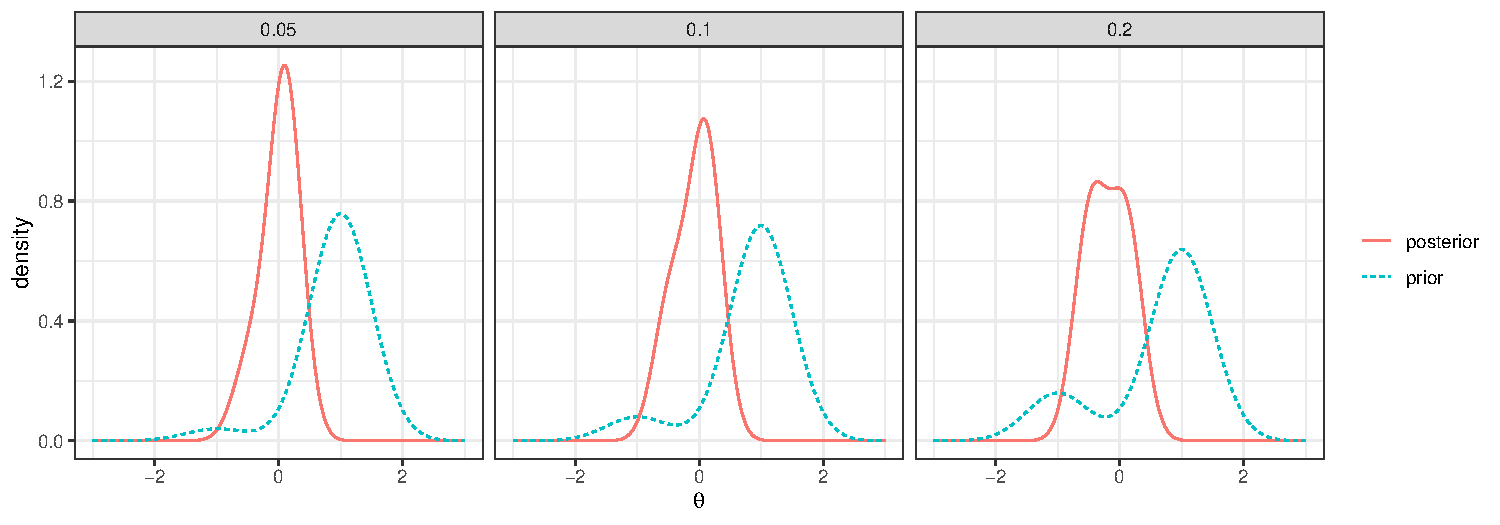
\includegraphics[width=1.15\linewidth]{figures/normal_mixture_prior_posterior.pdf}
\end{figure}

\scriptsize
\begin{minted}{R}

library(tidyverse)

y_bar = -0.25

post_mean_1 <- (0.25*y_bar + 0.1*1)/0.35
post_mean_2 <- (0.25*y_bar + 0.1*(-1))/0.35
post_std <- sqrt(1/14)

posterior_pi <-  function(pi) {
        pi*dnorm(y_bar,-1.0,sqrt(0.35))/((1-pi)*dnorm(y_bar,1.0,sqrt(0.35)) + pi*dnorm(y_bar,-1.0,sqrt(0.35))) }

plot_df_fun <- function(pi){
          data.frame(theta = seq(-3,3, length=1000)) %>%
           mutate(prior = (1-pi)*dnorm(theta, 1, 0.5) + pi*dnorm(theta, -1, 0.5),
                  posterior_pi = posterior_pi(pi),
                  posterior = (1-posterior_pi)*dnorm(theta, post_mean_1, post_std) +
                                  posterior_pi*dnorm(theta, post_mean_2, post_std),
                  pi=pi)}

plot_df <- bind_rows(lapply(c(0.2, 0.1, 0.05), plot_df_fun))

plot_df <- pivot_longer(plot_df, -c(theta,pi,posterior_pi), names_to="distribution", values_to="density")

ggplot(plot_df, aes(x=theta, y=density, col=distribution, linetype=distribution)) +
       geom_line() +
       xlab(expression(theta)) +
       theme_bw() +
       facet_grid(.~pi) +
       theme(legend.title=element_blank())
\end{minted}
\normalsize

\item This problem asks for an explicit expression of the mode of $\theta \mid \bar{y}$. It is just the $\argmax$ of the density in~\eqref{eq:bary_posterior}, which is easy to compute numerically. I do not think there is an analytic solution to the mode; indeed as per the figure above we see that the posterior could be bimodal as well. Here are a few things we can say (which we can verify e.g., by taking the derivative of the objective): the mode(s) must lie in $(\tilde{\mu}_2, \tilde{\mu}_1) = (-6.5/14, 1.5/14)$. Furthermore, as $\pi \to 0$, the mode converges to $1.5/14$ (I believe the answer the question writer was going for was $1.5/14$ and they meant to ask for an approximation of the posterior mode when $\pi$ is small). If you enjoy these kinds of calculations, also see~\citet{behboodian1970modes}.


\end{enumerate}

\subsection*{Problem 4: Assessing a clinical trial's conclusion}

Key ideas/tools:
\begin{itemize}
  \item Interaction effects in linear models.
  \item Intent-to-treat analyses.
  \item p-value interpretation.
\end{itemize}



\begin{enumerate}[label=(\alph*)]
\item Let us describe our main points of disagreement/agreement with the study:

\paragraph{Patients that dropped out:} A major issue with this study are the 51 patients that dropped out. If they had not dropped out, we would have a randomized experiment, and could even draw causal conclusions out of the two-sample comparison. Now, instead, we need to assume that the dropout of these patients was independent of their counterfactual (i.e., the response we would have observed, had they remained in their study). This may not be true, e.g., perhaps for some patients the drug has an adverse effect, and actually increases their blood glucose level. If these are these patients that dropped out, then the causal conclusions of the study will be flawed.

These situations arise all the time in medical studies, e.g., indeed, if a medication has side-effects on a patient, then it is not reasonable to expect them to keep taking that medication. However, there is a well-known remedy used: the investigators could have measured the glucose level at the end of the trial also for the patients that stopped taking the medication. Then we would use the measured response for these patients in an analysis, pooling them together with other treated patients. Such an analysis would produce an unbiased estimate of the treatment effect that however accounts for the (lack of) adherence of patients to the medication. This is called an \textbf{Intention-To-Treat  (ITT)} effect.

Unfortunately, here it seems the investigators did not/could not collect such intention-to-treat data. I would do a few sanity checks here (and perhaps report them as a sensitivity analysis in the manuscript's supplement): one check would be to conservatively ``impute'' a value for the patients that dropped out, say with $0$ (no change in glucose level), and rerun all analyses. If conclusions hold up even under a ``conservative'' , then we would be more confident in them. Another potential check would be to check if dropout is correlated with other patient-level variables (in case such data is available).

\paragraph{Reported effect and p-value:} The authors write that ``This study shows that the drug reduces glucose levels in subjects with moderately high glucose levels by more than placebo (t-test, $p < 0.0001$)'': It seems that this sentence refers to the two sample t-test that had a p-value of $0.0004$ which is not $< 0.0001$. Nevertheless, I mostly agree with this statement: modulo the patient drop-out considerations above, both the regression analysis and the two sample t-test support the conclusion that the drug reduced glucose level.

\paragraph{Interaction effects:} The authors further write that ``[the regression analysis] reveals that the drug is more effective in males than in females'': The coefficient for `sex` is not correctly interpreted here. The coefficient for `sex` hints that the decrease in glucose was stronger for males than females; across \emph{all} study subjects (i.e., whether treated or not). However it does not say anything about the relative effectiveness of the drug according to sex. The same erroneous interpretation is also applied to all other coefficients. Instead, one could try to answer the type of question asked here by including interaction effects in the regression, for example, \texttt{treatment * sex}. 

\paragraph{Study population:} The authors write ``we recommend that this drug be prescribed to every patient who wants to lower his/her glucose level." Critically, the study did not include diabetic patients who have high glucose levels and may be the most interested in taking the drug. Thus, recommending the drug to all potential patients seem premature without further study in this group. Even within the study population, the authors have not sufficiently backed up this claim. For example, they haven't shown evidence that the drug should be prescribed to both males and females, but they could easily add this evidence by conducting two t-tests, or fitting their regression model with an interaction term \texttt{treatment * sex}, and checking that the magnitude of the interaction term is smaller than the magnitude of the overall treatment effect.

\item Let us first outline concerns with the new study. In short, I do not believe the new study contradicts the first study.
\paragraph{p-values and power:} The major problem with this new study is that it misinterprets the p-value, i.e., it conflates the absence of evidence with the evidence of absence. While a small p-value provides evidence that we can reject the null hypothesis, a large p-value is uninformative: the p-value could be large either because the null is true or because the study is not powered sufficiently. Indeed; we only have a 12 vs. 12 comparison; a much smaller sample size than the first study. Furthermore, note that the p-value is still somewhat small and the authors of the new study commit the aforementioned fallacy and furthermore over-interpret the arbitrary cutoff of 0.05.
\paragraph{Generalizability:} The study recruitment criteria are slightly different than in the original study (e.g., start glucose levels 95-110 vs 100-120 in the original study, similarly for age) and so the populations of the two studies are also slightly different. However, I would not be worried too much about this here.

On the other hand, up to the small sample size, this appears like a nice randomized study that furthermore does not suffer from the dropout of the original study. I would thus start by looking at the 95\% confidence interval for $\mu_x - \mu_y$ in the new study. Even though we know that it will cross $0$, it would be promising to compare it to the confidence interval of the original study. Indeed, I think it is likely that the new confidence interval could provide further evidence for the effect found in the first study. One could also try to combine the two treatment effect estimates through a small meta-analysis (or if raw-data is available, use both studies in the same linear regression).	 

\end{enumerate}

\subsection*{Problem 5: Two ways of bootstrapping}
Key ideas/tools:
\begin{itemize}
  \item Time-series bootstrap.
  \item Bootstrapping individuals.
\end{itemize}

Statistician A's procedure does not make sense to me; there are some details missing from the description. Thus I think that this problem is quite open-ended and that the answer will depend on the interpretation of what Statistician A actually intends to do. Just make sure to describe in detail how you interpreted Statistician A, before providing an answer! In this solution we will assume that A's suggestion is to re-sample swimmer's with replacement.

One way to conceptualize what is going on, is as follows: there are two sources of variation in this dataset. First, swimmers are different from each other. Second, the time series measurements (i.e., the speed of the swimmers on 40 consecutive days) are also random; even when we only look at a single swimmer: each time they swim, there's a random source of variation determining how long it will take them to finish the 100 meters; and furthermore there is correlation across days: there could be hot-streaks, so that if a swimmer swims faster than expected on one day, they do so the next day too because of increased morale.

One way to formalize the two sources of randomness is through a hierachical model. First, for $i=1,\dotsc,100$ ( the 100 swimmers), we draw:
\begin{equation}
\label{eq:level1}
F_i \simiid \mathbb P,
\end{equation}
where $F_i$ is itself a probability measure on say $\RR^{41}$ and $\mathbb P$ is a probability measure on the space of probability measures. Here we assume that all the swimmers come from the same population that is described by $\mathbb P$.  At the second level of sampling, we draw for the $i$-th swimmer
\begin{equation}
\label{eq:level2}
(S_{it})_{1 \leq t \leq 41} \mid F_i\;\;  \sim \;\;F_i,
\end{equation}
and the statistician gets to observe $S_{it}, 1\leq t\leq 40$ and seeks to predict the $S_{i,41}$. 

Let us make this concrete by a simple random effects model. Say the only thing that differs across swimmers is the their mean speed $\mu_i$. Then the sampling could be described by the two-level model:
$$ \mu_i \sim \mathcal{N}(\nu, \tau^2),\;\;  S_{i\cdot} \mid \mu_i \sim \mathcal{N}(\mu_i, \Sigma),$$
for some $\nu, \tau^2, \Sigma$. This is not necessarily a good model, but it illustrates the more general two-level model described above; here the random distributions $F_i$ are equal to $F_i = \mathcal{N}(\mu_i, \Sigma)$. 


The difference between the two statisticians now can be described as follows: Statistician A  cares about the uncertainty induced from the sampling step in~\eqref{eq:level1}, while statistician B about the randomness in~\eqref{eq:level2}. 

Let us first discuss the two approaches assuming the model used to predict the 41st day is fixed and not trained based on the data at hand.

If we care about each swimmer individually, and want to assess uncertainty of the prediction individually for each swimmer, then we should follow the recommendation of Statistician B.\footnote{As an aside, it is perhaps worth noting a peculiarity in a time-series bootstrap when viewed in light of~\eqref{eq:level2}. We seek to represent uncertainty in $F_i$ based on a \emph{single} sample from $F_i$! This is only possible under strong assumptions, e.g., a parametric model assumption or the assumption that measurements taken multiple days apart are approximately independent.}

We would prefer an approach that samples swimmers (as suggested by Statistician A) if we care about the population of swimmers. For example, we could answer the following question: What is the average predicted speed across all possible swimmers in our population and what is our uncertainty? Then, we could resample swimmers with replacement (i.e., get $(S_{i_j\cdot})_{1\leq j \leq 100}$ with $i_j \in \cb{1,\dotsc,100}$), get the prediction for each, average these predictions to get an average prediction. We could repeat the sampling step multiple times and finally report a bootstrap percentile interval.

The suggestion of statistician A would also makes more sense if the model is trained on the swimmers themselves. For simplicity, let us consider a leave-one-out prediction scheme in which we are interested in predicting the speed of swimmer 1 on day 41 and train a model based on the other 99 swimmers. Then, keeping the time-series of swimmer 1 fixed, there is still randomness in the prediction because of the random selection of the other 99 swimmers. We could assess this uncertainty by resampling the 99 swimmers with replacement, building a new model each time and predicting the final speed of swimmer 1. An alternative here would be to combine the approaches of statisticians A and B: we could resample the other 99 swimmers with replacement to build a new predictive model, then use the time-series bootstrap to resample the data of swimmer 1, and finally predict the final speed of swimmer 1. Such a scheme would account for both sources of uncertainty. 








\subsection*{Problem 6: Population LASSO}

Key idea/tools:

\begin{itemize}
  \item Approximating the population objectives through empirical averages.
  \item The LASSO fit depends only on $\boldX^\top Y$ and $\boldX^\top \boldX$.
  \item Decomposing a covariance matrix through the Cholesky factorization or its eigenvalue decomposition. 
\end{itemize}


In this problem we are interested in solving the population LASSO problem,
\begin{equation}
\label{eq:population_lasso}
\argmin_{\beta} \frac{1}{2} \EE{\p{Y - X^\top \beta}^2} + \lambda \Norm{\beta}_1,
\end{equation}
where $(X,Y)$ are centered and have a known covariance matrix $\Sigma$. Instead, we have at our disposal a LASSO solver for the empirical objective:
\begin{equation}
\label{eq:empirical_lasso}
\argmin_{\beta} \frac{1}{2} \Norm{\boldY - \boldX^\top \beta}^2_2 + \lambda \Norm{\beta}_1,
\end{equation}
where $\boldX$ is a $N \times p$ design matrix with rows $x_i^\top$ and $\bold{Y}$ a $N\times 1$ response vector with entries $y_i$.

\begin{enumerate}[label=(\alph*)]

\item  Upon expanding the square of the population mean-squared error, we find that
\footnotesize
\begin{equation}
\label{eq:lasso_decomp}
\EE{\p{Y - X^\top \beta}^2} = \EE{Y^2 + \beta^\top  X X^\top  \beta -2 Y X^\top \beta} = \sigma_{YY} + \beta^\top \Sigma_{XX} \beta -2 \sigma_{XY}^\top \beta
\end{equation}
\normalsize
In particular, the solution of the optimization problem only depends on the covariance $\Sigma$ of $(X,Y)$. So for $i=1,\dotsc,N$ we could draw samples $(x_i, y_i)$ from a multivariate normal distribution with mean $0$ and the given covariance $\Sigma$. Then we could solve:

\begin{equation}
\label{eq:sample_lasso}
\min_{\beta} \frac{1}{2 N} \sum_{i=1}^N \p{y_i - x_i^\top \beta}^2 + \lambda  \Norm{\beta}_1
\end{equation}
For large enough $N$, by the law of large numbers, this would provide a good approximation to the population LASSO objective, since:
$$  \frac{1}{N} \sum_{i=1}^N \p{y_i - x_i^\top \beta}^2 \approx  \EE{y_i - x_i^\top \beta}^2, $$
where in light of~\eqref{eq:lasso_decomp} the approximation can be made uniform in $\beta$ (say for $\beta$ in a compact set; and we can check that for $\lambda > 0$ the optimal $\beta$ for the population problem indeed lies in a compact set). 

To use our friend's software we would use the pairs $(x_i, y_i)$ as input and set the penalty parameter to $N \cdot \lambda$. 

Let us provide a few more details on drawing samples from the specified multivariate normal distribution. Let $\Sigma = LL^\top$ be the Cholesky decomposition of $\Sigma$\footnote{Instead of the Cholesky decomposition, we could have have used the Eigendecomposition $\Sigma = VD^2V^\top$ and then proceeded as above with $L=VD$.} Then let $u_i^j \simiid \mathcal{N}(0, 1),\; j=1,\dotsc,p+1$, $u_i = (u_i^1, \dotsc, u_i^{p+1})$ and set:
$$ (x_i, y_i) = z_i = Lu_i$$
Then indeed $(x_i, y_i) \sim \mathcal{N}(0, \Sigma)$.
\item This question is phrased in a somewhat confusing way. My interpretation is as follows: let us assume we can solve~\eqref{eq:sample_lasso} exactly, i.e., let us ignore floating point arithmetic errors. Then, can we use~\eqref{eq:sample_lasso} to exactly solve~\eqref{eq:population_lasso}? It turns out that we can achieve this with what amounts to the computational shortcut for kernel learning~\citep{hastie2004efficient} when $p>n$.

Let $\Sigma = LL^\top$. This could be for example the Cholesky decomposition of $\Sigma$ (as explained for sampling in part a; also see footnote therein). Then let $\boldY$ be the last row of $L$ and $\boldX^\top$ the $p \times p+1$ matrix consisting of the first $p$ rows of $L$. We can think of this procedure as providing as with pseudoobservations $(x_i, y_i)$.

Note that by expanding as we did in~\eqref{eq:lasso_decomp} for the population objective, we get
\begin{equation}
\label{eq:sample_lasso_expanded}
 \Norm{\boldY - \boldX^\top \beta}^2_2  = \Norm{\boldY}_2^2 -2\boldY^\top \boldX\beta + \beta \boldX^\top \boldX\beta 
\end{equation}

However, by construction, we have that $\boldX^\top \boldX = \Sigma_{XX}$,  $\Norm{\boldY}_2^2 = \sigma_{Y}$ and $\boldX^\top \boldY = \sigma_{XY}$, so that these problems are the same.

\end{enumerate}

% \newpage
% \section{Applied 2020: Solution\footnote{Isaac Gibbs, Dan Kluger and M.H.}}

\subsection*{Problem 1: Maximum Likelihood for Truncated Data}

\begin{enumerate}
\item[a)]
Both \verb|t.test(Y)| and \verb|lm(Y ~ 1)| compute the mean and standard deviation $Y$. This is not possible without observing the full dataset. By default, both of these functions will simply ignore the missing values. This will cause us to overestimate the mean of $Y$ and produce a confidence interval that is biased upwards.
\item[b)]
The methods in part a) give estimates that have a positive bias. To derive a likelihood based method let $Z_1,\dots,Z_n$ denote the latent values of the light emissions. We are told that $Z_i \sim N(\mu,\sigma^2)$ for some unknown values $\mu$ and $\sigma^2$, and  we observe 
\[
Y_i = \begin{cases}
Z_i, \ \text{if } Z_i > C\\
\text{NA}, \text{ otherwise}
\end{cases}.
\] 
Let $\Phi$ and $\phi$ denote the cdf and pdf of $N(0,1)$, respectively. Let $\delta_i := \bone_{Y_i \neq NA}$. Then, the likelihood of the observed data is 
\[
p(Y;\mu,\sigma) = \prod_{i=1}^n \left( \frac{1}{\sigma} \phi\left( \frac{Y_i - \mu}{\sigma} \right) \right)^{\delta_i } \Phi\left( \frac{C - \mu}{\sigma} \right)^{1 - \delta_i} 
\]
and, up  to a constant, the log-likelihood is
\[\ell(\mu,\sigma) = \sum_{i=1}^n -\delta_i\left(\log(\sigma) -\frac{1}{2}\left(\frac{Y_i}{\sigma}-\frac{\mu}{\sigma}\right)^2\right) + (1-\delta_i)\log \Phi\left(\frac{C}{\sigma}-\frac{\mu}{\sigma}\right). \]
This is not a concave function of $(\mu,\sigma)$, but it is concave in the transformed parameter $\lambda = \frac{1}{\sigma}$ and $\nu = \frac{\mu}{\sigma}$. In these parameters, we have
\[\ell(\lambda,\nu) =\sum_{i=1}^n \delta_i\left(\log(\lambda) -\frac{1}{2}\left(\lambda Y_i-\nu\right)^2\right) + (1-\delta_i)\log \Phi\left(\lambda C-\nu\right). \]
This function is concave because is non-negative combination of concave functions. We can thus use Newton's method to find $\hat{\lambda},\hat{\nu}$ which we can transform to get $\hat{\sigma} = \frac{1}{\hat{\lambda}}$ and $\hat{\mu} = \frac{\hat{\nu}}{\hat{\lambda}}$.


% We could try to maximize this likelihood (or its log) to get estimates for $\mu$ and $\sigma$. There are multiple challenges to this optimization problem. The largest one is that the likelihood and the log-likelihood are both non-convex. Since we have only two parameters a grid search for the optimal values of $(\mu,\sigma)$ could be reasonable. Alternatively, we could try running gradient ascent. A small barrier to gradient ascent is that $\Phi(\cdot)$ has no closed form. However, this is only a minor obstacle since the gradient of $\Phi(\cdot)$ is known and the values of $\Phi(\cdot)$ can be computed numerically by evaluating a one-dimensional integral. Since the problem is non-convex we may want to run gradient ascent with many different random initializations. One potentially good initialization is to use the empirical mean and standard deviation of the observed $Y_i$ with the missing values replaced by $C$. If $C$ is not too large these should be reasonable starting estimates.

If you do not recognize the above transformation, a good alternative is to use EM. In the E-Step we would need to compute
\[
\mme_{\hat{\mu}^t,\hat{\sigma}^t}[\log(p(Z;\mu,\sigma) ) | Y].
\]
By expanding $\log(p(Z;\mu,\sigma) )$ we will find that it is sufficient to compute 
\[
 \mme_{\hat{\mu}^t,\hat{\sigma}^t}[Z_i | Y_i] \ \ \ \text{ and } \ \ \ \mme_{\hat{\mu}^t,\hat{\sigma}^t}[Z_i^2 | Y_i].
\]
If $Y_i \neq NA$ then $ \mme[Z_i | Y_i]  = Y_i$ and $\mme[Z_i^2 | Y_i] = Y_i^2$. Otherwise, computing these expectations reduces to computing the mean and variance of a truncated Gaussian, which is a straightforward computation that we could carry out. Finally, in the M-step we have to optimize $\mme_{\hat{\mu}^t,\hat{\sigma}^t}[\log(p(Z;\mu,\sigma) ) | Y]$ over $\mu$ and $\sigma$, which is a straightforward two dimensional calculus problem which yields:

$$\hat{\mu}^{t+1} = \frac{1}{n} \sum_{i=1}^n \mathbb{E}_{\hat{\mu}^t,\hat{\sigma}^t}[Z_i|Y_i] \quad \text{and} \quad (\hat{\sigma}^{t+1})^2 = \frac{1}{n} \sum_{i=1}^n \Big( \mme_{\hat{\mu}^t,\hat{\sigma}^t}[Z_i^2|Y_i] -2 \hat{\mu}^{t+1}  \mme_{\hat{\mu}^t,\hat{\sigma}^t}[Z_i|Y_i] + (\hat{\mu}^{t+1})^2 \Big)$$
\item[c)]
Intuitively we should have that the observed data $Y_1,\dots,Y_n$ come from a truncated normal distribution. Thus, we could maximize the likelihood
\[
p(Y;\mu,\sigma) = \prod_{i=1}^n \frac{1}{\sigma} \phi\left(\frac{Y_i - \mu}{\sigma}\right)\left( 1- \Phi\left(\frac{C - \mu}{\sigma}\right) \right)^{-1}.
\]
The log of this likelihood is no longer concave in $\lambda = \frac{1}{\sigma}$ and $\nu = \frac{\mu}{\sigma}$, and so we have to use an inexact method such a gradient descent with multiple initialization. Another option would be to do a grid search over $(\mu,\sigma)$.

Without doing any rigorous calculations (assuming both devices take measurements for the same amount of time) we suspect that the device in b) should give a better estimate of $\mu$ and $\sigma$ than the device in c). This is due to the fact that in b) we observe strictly more data than in c).

\textbf{Aside:} The question explicitly says that we do not need to do a rigorous calculation. However, seeing a rigorous calculation could still be informative. This calculation shows that the likelihood written out above is actually the conditional likelihood for the $Y_i$, conditional on the number of observations that we observe.

The calculation proceeds as follows. Let $Z_1,\dots,Z_m$ denote the latent non-truncated measurements of light brightness. Then, we observed $Z_{i_1},\dots,Z_{i_n}$ where $1 \leq i_1<i_2<\dots < i_n \leq m$ are the indices at which $Z_{i_j}  > C$. Note that $n$ is itself random here. Now, for any $x > C$ and $1 \leq i \leq n$ we have that  
\begin{align*}
 \mmp(Y_i > x | n = k)  = \sum_{i_1,\dots,i_k}  & \mmp(Y_i > x | n=k, Z_{i_1},\dots,Z_{i_k} > C, Z_j \leq C, \forall j \notin \{i_1,\dots,i_k\} )\\
& \cdot \mmp(Z_{i_1},\dots,Z_{i_k} > C, Z_j \leq C, \forall j \notin \{i_1,\dots,i_k\}|n=k) .
\end{align*}
Given fixed values for the indices $i_1,\dots,i_k$ let $j^*$ be the index such that $Y_i = Z_{i_{j^*}}$. Then,
\begin{align*}
& \mmp(Y_i > x | n=k, Z_{i_1},\dots,Z_{i_k} > C, Z_j \leq C, \forall j \notin \{i_1,\dots,i_k\} )\\
 & =  \frac{\mmp(Z_{j^*} > x, Z_{i_1},\dots,Z_{i_k} > C, Z_j \leq C, \forall j \notin \{i_1,\dots,i_k\} )}{\mmp(  Z_{i_1},\dots,Z_{i_k} > C, Z_j \leq C, \forall j \notin \{i_1,\dots,i_k\} )}\\
 & =  \frac{\left(1-\Phi\left( \frac{x-\mu}{\sigma}\right)\right)  \Phi\left( \frac{C-\mu}{\sigma}\right)^{m-k}   \left( 1- \Phi\left( \frac{C-\mu}{\sigma}\right)\right)^{k - 1} }{\Phi\left( \frac{C-\mu}{\sigma}\right)^{m-k}  \left(1- \Phi\left( \frac{C-\mu}{\sigma}\right)\right)^{k}} \\
 & = \frac{1-\Phi\left( \frac{x-\mu}{\sigma}\right) }{1-\Phi\left( \frac{C-\mu}{\sigma}\right) }.
\end{align*}
Differentiating this last expression gives the claimed formula for the likelihood.
\item[d)]
We are told to replace $\mu$ in the above likelihoods with $\mu_i = X_i^\top\beta$. Since we are given a function for the gradient of the log-likelihoods we can use gradient ascent to maximize the objective. Assuming that $\sigma^2$ is fixed and known the updates would look like 
\begin{equation}\label{2020Q1grad_desc}
\beta_{t+1} = \beta_t + \eta \text{grad\_log}(Y,X\beta_t,\text{sigma\_sq},C)^TX,
\end{equation}
where $\eta > 0$ is a fixed step-size parameter. If $\sigma^2$ is unknown then we would still use the update (\ref{2020Q1grad_desc}), but in this update we would only use the first $n$ coordinates of $\text{grad\_log}(Y,X\beta_t,\text{sigma\_sq},C)$, we would replace sigma\_sq with $\sigma^2_t$, and we would additionally have the update
\[
\sigma_{t+1} = \sigma_t + \eta \Big[ \text{grad\_log}(Y,X\beta_t,\sigma^2_t,C) \Big]_{n+1}.
\]
Finally, we could use the function logl($Y$,mu,sigma\_sq,$C$) to judge the results of gradient ascent with multiple different random initializations.
\end{enumerate}

\subsection*{Problem 2: Low-Rank Matrix Factorization}

\begin{enumerate}
\item[a)]
The goal is to find matrices $A \in \mmr^{T \times 13}$ and $B \in \mmr^{990 \times 13}$ that minimize $||X - AB^T||_2^2$. We know that the skinny SVD optimizes this objective. Namely, let
\[
X = \sum_{i=1}^{990} \sigma_i u_i v_i^T
\]
denote the SVD of $X$ where $\vert \sigma_1 \vert \geq \dots \geq \vert \sigma_{990} \vert \geq 0$. Then, we can take 
\[
\hat{A} = U_{1:13}\text{diag}(\sigma_1,\dots, \sigma_{13}) \ \ \ \text{ and } \ \ \ \hat{B}^T =  (V_{1:13})^T
\]
where $U_{1:13}$ and $V_{1:13}$ denotes the matrices with columns $u_1,\dots,u_{13}$ and $v_1,\dots,v_{13}$, respectively.
\item[b)]
The individual matrices $A$ and $B$ will not be unique. Namely, given an optimal solution $(A,B)$ we have that for any orthogonal matrix $O$, $AB^T = AOO^TB^T$ and thus $(AO,BO)$ is also a solution. On the other hand, $AB^T$ will be unique iff $\sigma_{13} > \sigma_{14}$ since in this case the skinny SVD is unique.
\item[c)]
Let $A_1,\dots,A_{T}$ denote the rows of $A$ and $B_1,\dots,B_{990}$ denote the rows of $B$. Then,
\[
||X - AB^T||_2^2 =  \sum_{i=1}^{T}  \sum_{j=1}^{990}   (X_{ij} - B_j^TA_i )^2.
\]
For each fixed value of $i \in \{1,\dots,T\}$ we recognize $ \sum_{j=1}^{990}   (X_{ij} - B_j^TA_i )^2$ as a linear regression problem with feature-response pairs $\{(B_j,X_{ij})\}_{1 \leq  j \leq 990}$. Using known results from linear regression this expression will be minimized by taking
\[
A_i = (B^TB)^{-1}B^Tx_i.
\]
By the separability of the objective function in $i$ it follows that for a fixed $B$, $A$ is optimized when setting $A^T = (B^TB)^{-1} B^T X^T$. Note that this assumes that $B$ is full-rank. If it is not full rank then you can replace the inverse by a pseudo-inverse.

\item[d)]
Using the same reasoning as in part c) we have that the minimizing value for $B$ will be given by
\[
B^T = (A^TA)^{-1} A^TX.
\]
Note that this assumes that $A$ is full-rank. If it is not full rank then you can replace the inverse by a pseudo-inverse.
\item[e)]
Letting $x_{T+1,\mathcal{O}}  \in \mathbb{R}^{990-45}$, denote the vector of observations at time $T+1$ with the entries dropped and let $B_{\mathcal{O}} \in \mathbb{R}^{(990-45) \times 13}$ denote the matrix $B$ with the rows which correspond to missing entries of $x_{T+1}$ removed. We could estimate $a_{T+1}$ be setting
\[
\hat{a}_{T+1} = \arg \min_{a} ||x_{T+1,\mathcal{O}} - B_{\mathcal{O}} a ||_2^2,
\]
As in parts c) and d) solving this optimization problem is equivalent to solving a linear regression problem and obtain that $\hat{a}_{T+1}=(B_{\mathcal{O}}^T B_{\mathcal{O}})^{-1} B_{\mathcal{O}}^T x_{T+1,\mathcal{O}}$. Then, we could estimate the missing values in the full vector by looking at the corresponding entries of $\hat{x}_{T+1} = B\hat{a}_{T+1}$. 
\end{enumerate}

\subsection*{Problem 3: Poisson GLMs}

\begin{enumerate}
\item[a)]
You can take $X$ to be the matrix with $n_i$ copies of row $x_i$ and $Y \in \mmr^{N}$ to be the vector with entries $y_{ij}$ and then use the R call glm($Y \sim X-1$, family=poission(link="log")).
\item[b)]
The likelihood for the data is 
\[
p(Y;X,\beta) = \prod_{ij} \frac{ \exp( y_{ij} x_i^T\beta - \exp(x_i^T\beta )) }{y_{ij}!} \propto \prod_i \exp(\sum_{j} y_{ij} x_i^T\beta - n_i\exp(x_i^T\beta)). 
\]
Additionally, note that $T_{i} := \sum_{j} y_{ij} \sim \text{Poisson}(n_i\exp(x_i^T\beta))$. So, the likelihood for $T_{1},\dots,T_{I}$ is 
\[
p(T_{1},\dots,y_{I};x_1,\dots,x_I,\beta) \propto \prod_i \exp(T_{i} x_i^T\beta - n_i\exp(x_i^T\beta)).
\]
In particular, we find that the likelihood for the data  $\{T_{i}\}$ is proportional to the likelihood for $\{y_{ij}\}$. Thus, maximum likelihood based inference will be the same for these two datasets.  Under, the current model we have that the mean of $T_{i}$ is $\mu_{i\cdot}$ with 
\[
\log(\mu_{i\cdot}) = \log(n_i) + x_i^T\beta
\] 
We recognize this as a GLM with offsets. Let $T =(T_1,\dots,T_I) \in \mmr^I$, $\tilde{X} \in \mmr^{I \times p}$ be the matrix with rows $x_i$, and $n = (n_1,\dots,n_I)$. Then, we find that the model from part a) can be fit using the GLM call glm($T \sim \tilde{X} - 1$,family=poisson(link="log"),offset=log(n)).

Note that your justification above need not explicitly write out the likelihood and could use a sufficient statistics argument instead. % in terms of the $T_1,\dots,T_I$ and you can simply say that the sum of $n_i$ IID Poissons with rate parameter $\lambda_i$ follows a $\text{Pois}(n_i \lambda_i)$ distribution and the sum a sufficient statistic for estimating $\lambda_i$.
\item[c)]
Extending our previous model it may now be reasonable to posit that the events for galaxy $i$ come from a homogeneous Poisson process with mean parameter $\exp(x_i^T\beta)$. i.e. we have that $y_{ij}$ are independent Poisson random variables with  
\[
\log(\mu_{ij}) = \log(\ell_{ij}) + x_i^T\beta. 
\]
We can fit this model using the call glm($Y \sim X-1$, family=poission(link="log"),offset = log($\ell$)) where $\ell$ is the vector of lengths and $Y$ and $X$ are as in part a).
\end{enumerate}

\subsection*{Problem 4: Estimating Starfish Diversity}

\begin{enumerate}
\item[a)]
$S_i$ will be larger for less diverse antibody pools. One way to see this is to observe that 
\[
S_i = \sum_{j=1}^J \hat{p}_{ij}^2 \leq \sum_{j=1}^J \hat{p}_{ij} = 1,
\] 
with equality for vectors $\hat{p}_{i \cdot}$ that satisfy $\hat{p}_{ij} = 1$ for some $j$ and $\hat{p}_{ij'} = 0$ for all other $j' \neq j$. i.e. $S_i$ is maximized by the least diverse antibody pools. Moreover, by Jensen's inequality we have that 
\[
S_i =  J  \sum_{j=1}^J \frac{\hat{p}_{ij}^2}{J} \geq J \left( \sum_{j=1}^J \frac{\hat{p}_{ij}}{J} \right)^2 = \frac{1}{J}
\]
with equality being obtained by the uniform distribution. i.e. $S_i$ is minimized by the most diverse populations. 
\item[b)]
Perhaps the largest issue with $S_H$ is that its value can be dominated by a single starfish that has very large counts for all antibodies. This is a major concern because we are told that "the absolute numbers $n_{ij}$ depend  a  lot  on  how  the  sample  was  taken,  and  so  the  ratios  are  considered  more useful." For a concrete example, suppose 9/10 of the starfish collected have very diverse antibodies and a relatively small total number of antibodies measured and the final remaining starfish does not have very diverse antibodies, but has a large total number of antibodies. Then, the value of $S_H$ will be dominated by the one non-diverse starfish and we will estimate that the population does not have a very diverse set of antibodies even though 9/10s of the starfish have a large diversity. Cases like this where some samples have larger total counts than others are common in many types of biological data (e.g. RNA-seq).

A better method would be to weight all of the starfish equally regardless of the magnitude of their total counts. To do this we could define 
\[
S_{H,i} = \sum_{j=1}^J \left( \frac{n_{ij}}{\sum_{j'=1}^J n_{ij'}} \right)^2
\]
to be the diversity measure for the $i_{th}$ high-salinity starfish and then define the new estimator 
\[
\tilde{S}_H = \frac{1}{10} \sum_{i=1}^{10} S_{H,i}.
\]
We could do the same thing for the low salinity starfish and compute the estimate $\tilde{S}_H - \tilde{S}_L$.

\item[c)]

Their bootstrap procedure does not appear to reflect the data generating mechanism and account for the clustered nature of their data. In particular, their bootstrap procedure treats each observed antibody in the high-salinity water as a sample, and samples the $\sum_j n_{H,j}$ antibodies with replacement. It does not account for the fact that the antibodies were measured by taking sampling antibodies in 10 different starfish (each of which could have different proportions of each antibody).

A better approach would be to use clustered bootstrap which resamples entire starfish with replacement but does not resample data within starfish (See Strategy 1 of Section 3.8 in \cite{davison_hinkley_1997}). You can think of this as a block bootstrap where each starfish is a block.  More specifically, for each $b=1,\dots,B$ we would obtain bootstrap datasets of starfish-level diversity scores $\{ S_{H,i}^b\}_{1 \leq i \leq 10}$ and $\{ S_{L,i}^b\}_{1 \leq i \leq 10}$ where $ S_{H,i}^b \sim \text{Unif}( S_{H,1},\dots, S_{H,10})$ and $ S_{L,i}^b \sim \text{Unif}( S_{L,1},\dots, S_{L,10})$. We would then use these datasets to get new estimates of the difference in means given by $$\tilde{S}_H^b - \tilde{S}_L^b = \frac{1}{10} \sum_{i=1}^{10} S_{H,i}^b -  \frac{1}{10} \sum_{i=1}^{10} S_{L,i}^b$$ and then form a confidence interval by looking at the empirical quantiles of $\{\tilde{S}^b_H - \tilde{S}^b_L\}_{1 \leq b \leq B}$ (see Section \ref{sec:the_standard_bootstrap}).

An alternative to the previous procedure is to use a clustered bootstrap, where you sample starfish with replacement, and subsequently resample the antibodies within each starfish with replacement (See Strategy 2 of Section 3.8 in \cite{davison_hinkley_1997}). In particular, for $b=1,\dots, B$, to construct the bootstrap dataset for the high-salinity starfish, sample 10 high-salinity with replacement $i_1,\dots,i_{10}  \stackrel{IID}{\sim} \text{Unif} \{1,\dots,10 \}$ then for $k=1, \dots,10$, compute $S_{H,k}^b$, by resampling the antibodies from starfish $i_k$ with replacement (this can be done by sampling a multinomial on $\{1 , \dots ,J \}$ with probabilities $\hat{p}_{i_k,j}$ with $\sum_{j} n_{i_k j}$ trials for the multinomial) and then using the resampled antibody counts in starfish $i_k$ to compute the diversity score $S_{H,k}^b$. You would do the same procedure to generate bootstrap samples of the diversity scores $S_{L,k}^b$  in the Low salinity waters. Finally you would let the $b$th bootstrap statistic be  $$\tilde{S}_H^b - \tilde{S}_L^b=\frac{1}{10} \sum_{k=1}^{10} S_{H,k}^b -  \frac{1}{10} \sum_{k=1}^{10} S_{L,k}^b,$$ and use the empirical quantiles of $\{\tilde{S}^b_H - \tilde{S}^b_L\}_{1 \leq b \leq B}$ to compute a bootstrap confidence interval.

While this is out of scope for quals, Section 3.8 in \cite{davison_hinkley_1997} recommends Strategy 1 over Strategy 2, but either would be an acceptable answer for quals.


%Their bootstrap procedure appears to be motivated by a Poisson model in which $n_{ij} \sim \text{Poisson}(\mu_j)$. While their procedure is valid in this context, it does not appear to be easy be rigorously justified under other models. 

%In particular, for part b) we proposed a new estimator 
%\[
%\tilde{S}_H - \tilde{S}_L = \frac{1}{10} \sum_{i=1}^{10} S_{H,i} -  \frac{1}{10} \sum_{i=1}^{10} S_{L,i}.
%\]
%This is just a difference in means estimator and thus the obvious way to estimate its null distribution is simply to re-sample starfish.



\end{enumerate}


\subsection*{Problem 5: EM for a Mixture of Regressions}

\begin{enumerate}
\item[a)] 
We have that 
\[
\log(p_{\theta}(Y)) = \sum_{i=1}^n \log\left(\sum_{j=1}^k \pi_j \frac{1}{\sqrt{2\pi\sigma^2}} \exp\left(-\frac{1}{2\sigma^2} \left(Y_i - a_j - b_jX_i\right)^2 \right) \right)
\]
and 
\begin{align*}
\log(p_{\theta}(Y,Z)) & = \sum_{i=1}^n \log\left( \pi_{Z_i} \frac{1}{\sqrt{2\pi\sigma^2}} \exp\left(-\frac{1}{2\sigma^2} \left(Y_i - a_{Z_i} - b_{Z_i}X_i\right)^2 \right) \right)\\
& = \sum_{i=1}^n \log(\pi_{Z_i}) - \frac{1}{2\sigma^2}  \left(Y_i - a_{Z_i} - b_{Z_i}X_i\right)^2 - \frac{1}{2}\log(2\pi\sigma^2)\\
& = \sum_{i=1}^n \left( \sum_{j=1}^k \left( \log(\pi_{j}) Z_{ij} - \frac{1}{2\sigma^2}  \left(Y_i - a_{j} - b_{j}X_i\right)^2 Z_{ij} \right)- \frac{1}{2}\log(2\pi\sigma^2) \right).
\end{align*}
There are $k$ independent parameters for the $a_j$'s, $k$ independent parameters for the $b_j$'s, $k-1$ independent parameters for the $\pi_j$, and one parameter for $\sigma$ for a total of $3k$ independent parameters.
\item[b)]
The notation here isn't very good. In order to run EM we will need to compute $\mme_{\tilde{\theta}}[\log(p_{\theta}(Y,Z))]$ not $\mme_{\theta}[\log(p_{\theta}(Y,Z))]$ where $\tilde{\theta}$ and $\theta$ are two potential values for the fitted parameters. Thus, I will re-define $\tau_{ij} = \mmp_{\tilde{\theta}}(Z_i = j|Y)$. This gives the expression
\begin{equation}\label{2020Q4_expect_ll}
\mme_{\tilde{\theta}}[\log(p_{\theta}(Y,Z))] = \sum_{i=1}^n \left( \sum_{j=1}^k \left( \log(\pi_{j})\tau_{ij} - \frac{1}{2\sigma^2}  \left(Y_i - a_{j} - b_{j}X_i\right)^2 \tau_{ij}  \right) - \frac{1}{2}\log(2\pi\sigma^2) \right).
\end{equation}
\item[c)]
The description of EM given in the problem statement is quite bad. The expression $\mme_{\theta,\tau}[\cdot]$ doesn't really make any sense and should be $\mme_{\hat{\theta},\tau}[\cdot]$. Regardless we will solve the problem ignoring the notational issues using the correct version of the EM algorithm. The goal is to optimize (\ref{2020Q4_expect_ll}) over $(a,b,\pi,\sigma)$ (strangely the question does not ask us to optimize $\pi$, but $\pi$ is part of $\theta$ so we certainly need to optimize over it). Optimizing over $\pi$ is a straightforward Lagrange multipliers calculation from which you should find that 
\[
\hat{\pi}_j = \frac{ \sum_{i=1}^n \tau_{ij}}{\sum_{k=1}^K \sum_{i=1}^n \tau_{ik}} = \frac{ \sum_{i=1}^n \tau_{ij}}{n},
\]
where one easily checks that from the definitions we must have that $\sum_{j=1}^K \tau_{ij} = 1$ for all $i$. Optimizing $a_j$ and $b_j$ splits into $K$ standard weighted least squares problems. Let $T_j = \text{diag}(\tau_{1j},\dots,\tau_{nj})$ and let $X= \begin{bmatrix} \bm{1} & (X_i)_{i=1}^n \end{bmatrix}$. Then, we have that 
\begin{align*}
& \left( \begin{matrix}
 \hat{a}_j \\ \hat{b}_j
\end{matrix} \right) = (X^TT_jX)^{-1} X^TT_jY\\
& = \frac{1}{(\sum_{i=1}^n \tau_{ij} X_i^2)(\sum_{i=1}^i \tau_{ij}) - (\sum_{i=1}^n \tau_{ij}X_i)^2}\\
& \ \ \ \ \ \cdot \left( \begin{matrix}
(\sum_{i=1}^n \tau_{ij} X_i^2)(\sum_{i=1}^i \tau_{ij}Y_i) - (\sum_{i=1}^n \tau_{ij}X_i)(\sum_{i=1}^n \tau_{ij}X_iY_i) \\ (\sum_{i=1}^n \tau_{ij})(\sum_{i=1}^i \tau_{ij}X_iY_i) - (\sum_{i=1}^n \tau_{ij}X_i)(\sum_{i=1}^n \tau_{ij}Y_i)
\end{matrix} \right) 
\end{align*}
Finally, by differentiating in terms of $\sigma^2$ and re-arranging one can easily compute that 
\[
\hat{\sigma}^2 = \frac{1}{n} \sum_{i=1}^n \sum_{j=1}^k (Y_i - \hat{a}_j - \hat{b}_jX_i)^2 \tau_{ij}.
\]
\item[d)]
The correct way to compute BIC is to use the \textbf{observed} data log-likelihood. This gives the value
\[
\text{BIC} = 3k\log(n) + 2\cdot 116.36 = 9\cdot\log(39) + 2\cdot 116.36 \approx 265.7.
\]
\item[e)]

In our setting there are $n=39$ samples and $k=3K$ independent parameters, so we can use the definition of AIC and BIC to compute the AIC and BIC values for $K \in \{1,\dots,5 \}$ in the table presented below. AIC is minimized at $K=5$ so AIC selects $K=5$ (or it could select $K>5$ depending on un-presented log likelihood values) . On the other hand the BIC  is minimized at and selects $K=4$. There are many different alternative ways to select the number of clusters. One option is to use information in the forestry literature to set a prior on $K$ and also a prior on $\theta \mid K$ and then compute the mode of the posterior distribution of $K$ given the data. %For example, we could hard threshold the clustering by assigning each $Y_i$ to the cluster that maximizes $\tau_{ij}$ at the fitted value of $\theta$ and then choose the value of $K$ that minimizes the within-cluster sum of squares.
\end{enumerate}

\begin{center}
\begin{tabular}{|| l l l l l l l ||} 
 \hline
 Method & Formula & $K=1$ & $K=2$ & $K=3$  & $K=4$ & $K=5$ \\ [0.5ex] 
 \hline
AIC & $6K-2 \log p_{\hat{\theta}}(Y)$ & 294.08 & 270.38 & 250.72  & 241.56 & 239.16 \\
 \hline
 BIC & $3K \log(39)-2 \log p_{\hat{\theta}}(Y)$ & 299.0707 & 280.3614 & 265.6921  & 261.5227 & 264.1134 \\
 \hline
\end{tabular}
\end{center}

\subsection*{Problem 6: Estimating the Mutation Rate}

There are many possible models you could consider. Two obvious choices are a Poisson model and a linear model. In what follows I will answer parts a, b, and c separately for each of these two choices. \\

\noindent \textbf{Solution using a Poisson model}\\

\noindent One potential model is that the $d_{i,r}$ values are independent with 
\[
d_{i,r}|t_i - t_r \sim \text{Poisson}((t_i-t_r)\mu).
\]
One nice aspect of this model is that the variance of $d_{i,r}$ scales linearly in the mean, which seems consistent with what we observe in the plot of the data.  A straightforward calculation shows that this gives the maximum likelihood estimator 
\[
\hat{\mu} = \frac{\sum_{i=1}^n d_{i,r}}{\sum_{i=1}^n t_i - t_r}.
\]
This estimator is unbiased for $\mu$ and since it is a sum of independent random variables it should also be consistent under only mild assumptions on the times $t_i - t_r$. To do inference for $\mu$ we could form the standard confidence interval for the MLE. This would be valid as long as the Poisson model is accurate. If we want to avoid this parametric assumption an alternative is to use the fact that $\hat{\mu}$ is unbiased and an average of independent random variables and thus directly derive a CLT for $\hat{\mu}$. The main thing we will need here is an estimate of the variance of $\hat{\mu}$. We have that 
\[
\text{Var}(\hat{\mu}) = \frac{1}{(\sum_{i=1}^n t_i - t_r)^2} \sum_{i=1}^n \text{Var}(d_{i,r}).
\]
We know that $\text{Var}(d_{i,r}^2) = \mme[(d_{i,r} - (t_i-t_r)\mu)^2]$. Since $\hat{\mu}$ is consistent for $\mu$ a reasonable way to estimate this quantity is using the estimator
\[
\hat{\sigma}^2 =  \frac{1}{(\sum_{i=1}^n t_i - t_r)^2}  \sum_{i=1}^n (d_{i,r} - (t_i - t_r)\hat{\mu})^2.
\]
Finally we can use the normal approximation $\hat{\mu} \stackrel{\cdot}{\sim} N(\mu,\hat{\sigma}^2)$ to get a confidence interval for $\mu$.

One flaw in our model is that it assumes a Poisson distribution for the mutations. However, above we derived a non-parameteric method for computing a confidence interval for $\mu$ and thus this modelling assumption is not critical. A potentially larger issue is the presence of outliers in the dataset. In particular, we see that at some of the larger time points there are a few outlying points with very large numbers of mutations (note that a Pois(10) Random variable is 40 or larger with probability less that $10^{-12}$).  These points could have a large influence on the estimator $\hat{\mu}$ and thus heavily impact our estimate of the mutation rate. As a first step we should investigate how the data was collected and try to determine if there were any possible errors in the data collection process that could lead to these outlying points. Alternatively, maybe there is a biological mechanism that would tell us that some rare cases will deviate from the Poisson model presented. In both of these cases we might want to remove these outlying points from the dataset before fitting the model. If we think these outlying points are true data points that cannot be ignored then we could still use the above estimator $\hat{\mu}$. However, we should be conscious of the fact that these points may have an outsized influence on the estimator that will invalidate our normal approximation. To try to judge the size of the influence of these points we could compute $\hat{\mu}$ both with and without removing the outliers and report both values.

Another issue with our model assumption is the assumption of independent observations. In particular, it could be that many observations had a recent ancestor that is also in the data. For example, an observation in January 2020 may be correlated with its direct descendants in the data (if a virus observed in January 2020 has a relatively high hamming distance from from the original strain, it is likely the descendants of that virus also have a relatively high hamming distance from the original strain). It is hard to tell from the information given whether there will be a lot of dependency between the samples without domain knowledge or additional information beyond $d_{r,i}$, $t_i$ and $t_r$. That being said, even if the samples are correlated, the proposed estimator for $\mu$ should still be unbiased and consistent, but the confidence intervals would likely be too small. \\

\noindent \textbf{Solution using a linear model}\\

\noindent An alternative to fit a linear model
\[
d_{i,r} = (t_i-t_r)\mu + \epsilon_i.
\]
Intuitively, it is reasonable to expect that the variance of $\epsilon_i$ will be larger for larger times as there is more time for mutation events to occur and thus more time to accumulate deviations from the mean. From the plot of the data it looks like a reasonable model would be that $\text{Var}(\epsilon_i)$ increases linearly with time. Thus, we could model that $\text{Var}(\epsilon_i) = (t_i-t_r)\sigma^2$. Using weighted least squares this would give the estimator
\[
\hat{\mu} = \frac{\sum_{i=1}^n d_{i,r}}{\sum_{t=1}^n t_i-t_r},
\]
which is the same as the estimator from the Poisson model. All the considerations from the previous section still apply to this estimator. Here it is even more clear that we should not make standard modelling assumptions like $\epsilon_i \sim N(0,(t_i-t_r)\sigma^2)$ since we know that the $d_{i,r}$ are discrete. The normal approximation given in the previous section could still be a good way to form a confidence interval for $\mu$. 






% % \newpage
% \section{Applied 2021: Solution\footnote{D.K.}}

\textbf{Key Ideas/ Main Tools:} Unmeasured confounders, GLMs, offsets

\subsection*{Problem 1: Modeling association between vaccination and death rates for Covid-19}

\begin{enumerate}
\item[a)] It is essential to ask the researchers whether they know the population in each county because counties with higher populations will tend to have a higher death count irrespective of the vaccination rates. Also, if rural counties with low populations tend to have low vaccination rates, not accounting for county population can make vaccination seem less effective than it is. \newline Other questions worth asking the researchers are if there are any confounding variables that are likely to effect both vaccination rates and death rates, and if any of those confounding variables are measured. For example, the quality of the health care system in a county would effect both vaccination rates and deaths, so it would be worth asking if there are any measured variables that reflect the quality of the healthcare system in each county. Another example is the age demographics. The age demographics can influence both the death rate and the vaccination rate in a county, so it would be helpful to know if the researchers have any covariates that reflect age demographics (e.g. the percentage of the population above age 70 in each county). If the researchers mentions a large number of confounding that they have measurements for, I would ask the researchers to select the few most important ones based on their domain knowledge and would mention that they should choose much fewer than 20 variables to control for because there are only 20 samples.  \newline

In addition to asking about county population levels and whether there are measured confounder variables not presented in the table, it would be worthwhile to double check with the researcher that the deaths were counted after the vaccines were distributed (otherwise any analysis would be unable to say anything about the effect of vaccination rates on death rates). 


\item[b)] Suppose the researchers are able to provide you with the population counts $N_1,\dots,N_{20}$ of the 20 counties, and for each of the $20$ they can give you a vectors $z_1, \dots, z_{20}$ of the few most important measured confounder variables for each county (e.g. age demographics and health care system quality metrics). Also suppose that their death counts in each county, indeed only include deaths from a time period after most of the vaccinations were given.

Letting $d_i$ denote the number of deaths in county $i$, $v_i$ denote the vaccination rate, $x_i \equiv (v_i, z_i)$,  I would fit the following Poisson GLM with offsets $\alpha_i \equiv \log(N_i)$

$$d_i \stackrel{\text{Ind}}{\sim} \text{Poisson} (\mu_i) \quad \log(\mu_i)=\alpha_i + x_i^T \beta \quad \text{for } i=1,...,20.$$

After fitting the GLM (which can easily be done in R) using the glm function, I would look at the confidence interval for the first estimated coefficient $\hat{\beta}_1$. If the confidence interval only contains negative values, then we can conclude that the data suggests higher vaccination rates are associated with lower death rates when controlling for the confounders encoded in the $z_i$. 



\end{enumerate}

\subsection*{Problem 2: Finding an essential subset}

\textbf{Key Ideas/ Main Tools:} Group Lasso

\subsubsection*{Defining the optimal essential subset as a solution to an optimization problem}

Observe that one way to obtain an essential subset is to find the matrix $B \in \mathbb{R}^{750 \times 750}$ that minimizes $\vert \vert R - R B \vert \vert_{F}^2$ subject to the constraint that only 25 of the rows of $B$ are allowed to have nonzero entries. More formally, letting $B[i,]$ denote the ith row of the matrix $B$ we could get an essential subset by solving the following optimization problem on $B$: $$\boxed{\text{minimize} \quad \vert \vert R - R B \vert \vert_{F}^2 \quad \text{ subject to } \quad \sum_{i=1}^{750} I \{ B[i,] \neq \mathbf{0} \} \leq 25 , B \in  \mathbb{R}^{750 \times 750} }.$$ Let $\tilde{B}$ be the solution to the above optimization problem and $\mathcal{S} = \{ i \in [750] \ : \ \tilde{B}[i,] \neq \mathbf{0} \}$, (that is let $\mathcal{S}$ be the indices of the nonzero rows of the solution $\tilde{B}$).   $\mathcal{S}$ will give an essential subset, as each portfolio (represented by a column in $R$) will be reasonably well approximated by a linear combination of the portfolios of at most . \footnote{Technically, to be an essential subset, we only desire that portfolios not in $\mathcal{S}$ are well approximated by linear combinations of portfolios in $\mathcal{S}$, but trivially, portfolios in $\mathcal{S}$ can be written as exact linear combinations of portfolios in $\mathcal{S}$ and do not contribute to the loss function $\vert \vert R - R B \vert \vert_{F}^2$.}  \newline

Solving the boxed optimization problem and setting $\mathcal{S}$ to be the nonzero rows of the solution will recover an essential subset of size at most 25, but unfortunately the optimization problem is nonconvex (it has an $l_0$ type constraint).


\subsubsection*{A tractable approach using the Group Lasso}


One way to induce a sparse number of nonzero rows of $B$ is to use the Group Lasso. In particular, for each $\lambda>0$, the Group Lasso can be used to solve the following convex optimization problem of finding:

$$\boxed{\hat{B}_{\lambda} \in \argmin_{B \in \mathbb{R}^{750 \times 750}} \Big( \frac{1}{2}  \vert \vert R - R B \vert \vert_{F}^2 + \lambda \sum_{i=1}^{750} \vert \vert B[i,] \vert \vert_2 \Big).}$$

We can solve this group Lasso problem for many different $\lambda$ values until we find a solution $\hat{B}_{\lambda}$ which has exactly 25 rows which have nonzero. In particular, letting $\hat{\mathcal{S}}_{\lambda}=  \{ i \in [750] \ : \ \hat{B}_{\lambda}[i,] \neq \mathbf{0} \}$, we can do a grid search on $\lambda$ until we find a $\lambda_*$ for which $\vert \hat{\mathcal{S}}_{\lambda_*} \vert =25$. Then we can report $\hat{\mathcal{S}}_{\lambda_*}$ to our boss as an essential subset. Note that this may not be the optimal essential subset in the sense of minimizing $\vert \vert R - R B \vert \vert_{F}^2$ subject to 25 nonzero rows of $B$; however, it will still be an essential subset according to your bosses definition (that any portfolio in not in $\hat{\mathcal{S}}_{\lambda_*}$ can be well approximated by a linear combination portfolios in $\hat{\mathcal{S}}_{\lambda_*}$).



\textbf{Additional References}: In some years, the Group Lasso is covered in the 305 coursework's lecture notes\footnote{https://web.stanford.edu/class/stats305c/notes/Regression/Sparse.html}, but it is not covered every year. See \cite{GroupLasso2013Obozinski} for a reference on the Group Lasso and some its theoretical guarantees in recovering a sparse set of rows.


\subsection*{Problem 3: Constructing Conformal Prediction Intervals}

\textbf{Key Ideas/ Main Tools:} Prediction Intervals, Conformal Inference, Exchangeability


\begin{enumerate}
\item[a)] The defining property of the prediction interval is that $\mathbb{P} \big(Y_{n+1} \in [L,U]  \big) \geq 1-\alpha$, where $\mathbb{P}$ is the joint distribution of the $n+1$ data points $(X_1,Y_1),\dots, (X_{n},Y_n),(X_{n+1},Y_{n+1})$

\item[b)] This procedure is not reasonable because the more you overfit the data, the smaller the predictions intervals will be. Ideally our prediction will not be overconfident about overfit predictions. In an extreme case suppose that $X_1, \dots, X_n$ are all distinct and that $\hat{\mu}$ is the best fit $n-1$ degree polynomial to the first $n$ datapoints. In this case, $\hat{\mu}(X_i)=y_i$ for all $i \in [n]$ implying that the residuals $r_1,\dots,r_n$ are all equal to zero, further implying that the proposed prediction interval will have width zero. Clearly, if we overfit the data, the true prediction interval shouldn't have width zero for a new point $X_{n+1}$.

\item[c)] Let $\mathcal{S} = \{ y \in \mathbb{R} \ : \ \pi(y) \leq (1- \alpha)(n+1)/n \}$ and let $L = \inf S$ and $U = \sup S$. To show that this gives a valid prediction interval first note that
$$\begin{aligned}
\mathbb{P} (Y_{n+1} \in [L,U] ) & \geq \mathbb{P} (Y_{n+1} \in \mathcal{S} )
\\ & =  \mathbb{P} ( \pi(Y_{n+1}) \leq (1- \alpha)(n+1)/n )
\\ & = \mathbb{P} \Big( \frac{1}{n} \sum_{i=1}^n I \{ R_{Y_{n+1}, i} \leq R_{Y_{n+1}, n+1} \} \leq (1- \alpha)(n+1)/n   \Big)
\end{aligned}$$


To simplify the above expression with an exchangeability argument, first define $\tilde{\mu}$ to to the curve fit to the $n+1$ data points $(X_1,Y_1), \dots,(X_n,Y_n), (X_{n+1},Y_{n+1})$.  Next, define for $i=1,\dots,n+1$,  $V_i \equiv  \vert Y_i - \tilde{\mu}(X_i) \vert$. Observe that since $(X_1,Y_1), \dots, (X_n,Y_n)$ , $(X_{n+1},Y_{n+1})$ are IID and  $\tilde{\mu}$ is function of the collection of these $n+1$ data points, $V_1,V_2,\dots,V_n,V_{n+1}$ is an exchangeable sequence of random variables. In addition, since $\tilde{\mu}(\cdot)=\hat{\mu}_{Y_{n+1}}(\cdot)$, $$ V_i \equiv  \vert Y_i - \tilde{\mu}(X_i) \vert = \vert Y_i -\hat{\mu}_{Y_{i+1}}(X_i) \vert =R_{Y_{n+1},i}.$$

Combining this with a previous result and using the exchangeability of $(V_i)_{i=1}^{n+1}$ (and assuming that almost surely $V_i \neq V_j$ for $i \neq j$), 
$$\begin{aligned}
\mathbb{P} (Y_{n+1} \in [L,U] ) & \geq  \mathbb{P} \Big( \frac{1}{n} \sum_{i=1}^n I \{ R_{Y_{n+1}, i} \leq R_{Y_{n+1}, n+1} \} \leq (1- \alpha) (n+1)/n   \Big)
\\ & = \mathbb{P} \Big( \frac{1}{n} \sum_{i=1}^n I \{ V_i \leq  V_{n+1} \} \leq (1- \alpha)(n+1)/n   \Big)
\\ & = \mathbb{P} \Big( \sum_{i=1}^n I \{ V_i \leq  V_{n+1} \} \leq (n+1) (1- \alpha)  \Big)
\\ & \geq \mathbb{P} \Big( \sum_{i=1}^n I \{ V_i \leq  V_{n+1} \} \leq \lfloor (n+1) (1- \alpha) \rfloor  \Big)
\\ & = \mathbb{P} \Big( \text{Unif}\{0,1,\dots,n-1,n \} \leq \lfloor (n+1) (1- \alpha) \rfloor  \Big)
\\ & = \frac{1+\lfloor (n+1) (1- \alpha) \rfloor}{n+1}
\\ & \geq 1-\alpha.
\end{aligned}$$
%
Above the step where $\sum_{i=1}^n I \{ V_i \leq  V_{n+1} \sim  \text{Unif}\{0,1,\dots,n-1,n \} $ follows from exchangeability of $(V_i)_{i=1}^{n+1}$ (and the assumption almost surely $V_i \neq V_j$ for $i \neq j$).

Note you can also cite Lemma's or Theorem's from Lecture 17 in Stats 300C to solve this problem.
\item[d)] If $X_{n+1}$ is far outside the range of the training data, I would be concerned that the assumption that $(X_1,Y_1), \dots,(X_n,Y_n), (X_{n+1},Y_{n+1})$ are exchangeable from some distribution $P$ is violated and that the intervals from part (c) are no longer valid. Even if $X_{n+1}$ was technically a draw from $P$, the collaborator may have taken many draws from $P$ and selected $X_{n+1}$ as an outlier draw from $P$, in which case the exchangeability assumption would also be violated. \newline

Despite failure to meet the exchangeability assumption, if we went ahead and constructed the prediction intervals defined in (c), we would get prediction intervals with undesirable behavior. In particular, if the curve $\hat{\mu}$ is fit based on kernel smoothing or local linear regression (and only considers points with similar $X$ values), then it would follow that for all $y$, $\hat{\mu}_y(X_{n+1})= y$ implying that $R_{y,n+1}=0$ for all $y$, further implying that $\pi(y)=0$ for all $y$. Therefore, if $\hat{\mu}$ is fit based on kernel smoothing or local linear regression, the prediction interval would have infinite length. If on the other hand the curve $\hat{\mu}$ is fit based on a global polynomial regression, one would expect $R_{y,n+1}$ to be much larger than $R_{y,i}$  ($i <n$) for most $y$ values in which case the prediction interval would be very small. However, for a global model, since the global model is unlikely to hold for outliers we would want the prediction intervals to be very large. In summary, if we were to fit a curve with large extrapolation bias, the interval from part (c) would be very small and not reflect the extrapolation bias, but if we were to fit a local smooth model, the intervals from part (c) would be infinite length. The collaborator should therefore expect meaningless intervals if they went ahead and used prediction intervals for their outlier point. 

\end{enumerate}



\subsection*{Problem 4: PCA versus k-means}

\begin{enumerate}

\item[a)] 
\textbf{Explanation for PCA:} Suppose that each of the features is centered such that columns of $X$ each have mean $0$. PCA can be thought of in terms of matrix factorizing $X$. In particular to implement PCA, you take the SVD of $X$, which is a matrix factorization given by $X=UDV^T$ where $U \in \mathbb{R}^{n \times n}$ and $V \in \mathbb{R}^{p \times p}$ are orthogonal matrices, and $D_{ij} = 0$ for all $i \neq j$ and $\vert D_{11} \vert \geq \vert D_{22} \vert \geq \dots \geq 0$. In PCA, the principal component directions are given by the columns of $V$, while the principal component scores are given by $UD$. Since $X=(UD) V^T$, principal component analysis can be thought of as factorizing $X$ into matrix of the principal component scores (given by $UD$) and a matrix whose rows are the principal component directions (given by $V^T$).

\textbf{Explanation for K-means:} K-means can be thought of as an approximate matrix factorization of $X \in \mathbb{R}^{n \times p}$. In particular let $$\mathcal{C}_K \equiv \Bigr\{ C \in \mathbb{R}^{n \times K} \ : \ C_{ij} \in \{0,1 \} \ \forall_{i \in [n],j \in [K]}, \sum_{j=1}^{K}C_{ij} =1 \ \forall_{i \in [n] } \Bigr\},$$

be the collection of $n \times K$ matrices whose rows contain exactly $K-1$ zeros and $1$ one. We can then think of K-means as solving the following approximate matrix factorization problem $$(\hat{C}, \hat{Z} ) = \argmin\limits_{C \in \mathcal{C}_K , Z \in \mathbb{R}^{K \times p} } \vert \vert X - CZ \vert \vert_F^2.$$

In particular, if you solve the above approximate matrix factorization problem, the $K$ rows of $\hat{Z}$ will give the $K$ cluster centroids for $K$-means, and the column index of the nonzero entry in each of the $n$ rows of $\hat{C}$ will give the cluster assignment for each of the $n$ points in the $K$-means algorithm (or put another way, $\hat{C}_{ij}$ is a indicator of whether the $i$th point is assigned to cluster $j$ in the K-means algorithm).

\item[b)] For PCA, you can determine the matrix $V$, whose columns give the principal components dierections using $X_{\text{train}}$. Then, you can use the principal component scores on your test set given by $X_{\text{test}} V$ as features (or some subset of the principal component scores as features) for predicting $Y_{\text{test}}$. Note that if your prediction method is linear regression, and only the first $k$ principal component scores are used as features, this approach would be principal components regression.

For $K$-means, you use the training data $X_{\text{train}}$, to determine the $K$ cluster centroids. Once you have the cluster centroids, you can determine the cluster assignment of each observation in the test set by determining which of the $K$ cluster centroids is closest (in Euclidean distance) to each row of the matrix $X_{\text{test}}$. Once you have the cluster assignments on the test set, you can use the cluster assignments as a categorical feature for prediction $Y_{\text{test}}$ (you may want to use other features in addition to the cluster assignment). 


You can evaluate the error in predicting $Y$ for your choice of prediction algorithm and your choice features using cross-validation on the set $(X_{\text{test}}, Y_{\text{test}})$.


\item[c)] While my peer isn't wrong that the cluster structure they found is predictive of $Y$, it is just not such an impressive predictor of $Y$. In particular my peer's cluster assignments give a statistically significant improvement over just using the grand mean of $Y$ for predicting $Y$. That being said, looking at the sum of squares in the ANOVA table, using the cluster means to predict $Y$ doesn't give an impressive improvement over using the grand mean to predict $Y$. In a similar vein, from linear regression on the cluster we also see that the residuals from the linear regression tend to be much larger in absolute value than the estimates of $Y$ for each cluster. So, I agree with my peer that the cluster structure found is predictive of $Y$, but it doesn't appear to be terribly important structure for predicting $Y$.

\item[d)] The results don't contradict each other so it does not cause me to doubt my peer's results. It is possible that the first first 5 principle components are simply not that associated (in a linear way) with the outcome variable $Y$. Perhaps the jth principal component for $j>5$ is important in predicting $Y$. Perhaps the 1st principal component is important in explaining $Y$, but it has $U$ shaped quadratic relationship with $Y$ with a linear coefficient of $0$. In either case the 3-means approach that my friend did would give a better prediction of $Y$ than the principal components regression approach (with 5 components) that I took.

While it doesn't sound like my peer did anything wrong, I'm not terribly impressed by his results because the structure he found is quite a weak predictor of $Y$ (admittedly, I am even less impressed by my own results). I would suggest to our supervisor that we continue seeking an alternative to the 3-means approach, as there likely is a better choice of features out there. Perhaps it would be an 8-means approach or involve more than the first 5 principal components or it would involve interaction terms. Also neither of our approaches leveraged the $Y_{\text{train}}$ data, even though we are told that it exists. I would therefore try to convince our supervisor that it is worth digging deeper before sticking to the 3-means approach of my peer.
\end{enumerate}


\subsection*{Problem 5: Testing and inference on a censored Gaussian draw}

\textbf{Key Ideas/ Main Tools:} Score test, maximum likelihood estimation, Bayesian inference

\begin{enumerate}
\item[a)] $Z$ is distributed as $N(\mu,1)$ variable constrained to be at least 2. Therefore, letting $\Phi$ denote the standard Gaussian CDF and $\phi$ denote the standard Gaussian pdf the likelihood is given by 

$$L(\mu)  = \frac{\frac{1}{\sqrt{2 \pi} } \exp \big( -\frac{1}{2} (Z- \mu)^2 \big)}{\int_{2}^{\infty} \frac{1}{\sqrt{2 \pi} } \exp \big( -\frac{1}{2} (z- \mu)^2 \big) \text{d}z} = \frac{\phi(Z-\mu)}{1- \Phi(2-\mu)} = \frac{\phi(Z-\mu)}{\Phi(\mu-2)}.$$

The loglikelihood is thus given by $$l(\mu) = \log \big( L(\mu) \big) = \log \big( \frac{1}{\sqrt{2 \pi}} \big) -\frac{1}{2} (Z- \mu)^2  - \log \big( \Phi(\mu-2) \big).$$
The score function is therefore given by $$U(\mu) =l'(\mu) = (Z-\mu) - \frac{\phi(\mu-2)}{\Phi(\mu-2)},$$ and the Fisher information is given by 

$$\begin{aligned} I(\mu) & = -\mathbb{E}[l''(\mu) \mid \mu] \\ & = -\mathbb{E} \Big[ -1  - \frac{\Phi(\mu-2) \phi'(\mu-2)-[\phi(\mu-2)]^2}{[\Phi(\mu-2)]^2 } \mid \mu \Big] \\ & =1+\frac{(2-\mu) \Phi(\mu-2) \phi(\mu-2)-[\phi(\mu-2)]^2}{[\Phi(\mu-2)]^2}.
\end{aligned}$$

To conduct a score test of the hypothesis $H_0: \mu=0$, one would use the test statistic, $$T= \frac{[U(0)]^2}{I(0)} = \frac{\big( Z - \frac{\phi(-2)}{\Phi(-2)} \big)^2}{1+\frac{2 \Phi(-2) \phi(-2)-[\phi(-2)]^2}{[\Phi(-2)]^2}}= \frac{(Z-r)^2}{1+2r-r^2} \quad \text{ where } r=\frac{\phi(-2)}{\Phi(-2)} \approx 2.373.$$

The score test will reject whenever $T$ exceeds $c_{1-\alpha}$, where $c_{1-\alpha}$ is the $1-\alpha$ quantile of a chi-squared distribution with one degree of freedom chosen to satisfy $\mathbb{P}(\chi_1^2 \leq c_{1-\alpha} )=1-\alpha$. (Note $c_{1-\alpha} \approx 3.84$ for $\alpha=0.05$). Thus the score test rejects whenever $$ T> c_{1-\alpha} \Leftrightarrow   \frac{(Z-r)^2}{1+2r-r^2} >  c_{1-\alpha} \Leftrightarrow  Z > r+ \sqrt{(1+2r-r^2) c_{1-\alpha}}  \text { or } Z<  r- \sqrt{(1+2r-r^2) c_{1-\alpha}}.$$

Since $Z< 2$ cannot be observed, at level $\alpha=0.05$, noting that $c_{0.95} \approx 3.84$, the score test of $H_0$ rejects whenever $$Z > r+ \sqrt{(1+2r-r^2) c_{1-\alpha}} \approx 3.036.$$


\item[b)] Since we just have to optimize over a 1-dimensional parameter you can use grid search to find the MLE. While the following argument is probably unneccasary for the applied qual, to double check that grid search can be used we will find $a, b \in \mathbb{R}$ such that we know $\argmax_{\mu \in \mathbb{R}} l(\mu) \in [a,b]$. Note that whenever, $\mu > Z$, $l'(\mu) <0$, so the MLE must be at most $Z$, and we can set $b=Z$. To find a lower endpoint $a$ for the grid search observe that as a consequence of Theorem 1.2.3 in Durrett, for $x<-1$, $\frac{\phi(x)}{\Phi(x)} \leq (\frac{1}{-x} -\frac{1}{-x^3} )^{-1}$

and hence for $\mu < 1$,
$$\begin{aligned}
l'(\mu) & = Z - \mu - \frac{\phi(\mu-2)}{\Phi(\mu -2)}
\\ & \geq Z - \mu -  \Big(\frac{1}{-(\mu-2)} -\frac{1}{-(\mu-2)^3} \Big)^{-1}
\\ & = Z - \mu - \frac{(2-\mu)^3}{(2-\mu)^2 -1 }
\\ & = Z - \mu - \frac{(2-\mu)^2}{(3-\mu) (1-\mu) } (2-\mu)
\\ & = Z -2 \frac{(2-\mu)^2}{(3 -\mu) (1-\mu)} + \frac{\mu(2-\mu)^2 -\mu (3-\mu) (1-\mu)}{ (3-\mu) (1-\mu)}
\\ & = Z -2 \frac{(2-\mu)^2}{(3 -\mu) (1-\mu)} + \frac{\mu }{ (3-\mu) (1-\mu)}.
\end{aligned}$$

Since the above inequality holds for any $\mu < 1$, it is easy to see that $\liminf\limits_{\mu \downarrow - \infty} l'(\mu) \geq Z-2 >0$. Further we can use the lower bound above to find an $a$ such that for all $\mu < a$, $$ l'(\mu) \geq Z -2 \frac{(2-\mu)^2}{(3 -\mu) (1-\mu)} + \frac{\mu }{ (3-\mu) (1-\mu)} >0.$$

Hence we have an interval $[a,b]$ for which $l'(\mu) >0$ when $\mu <a$ and $l'(\mu) <0$ when $\mu>b$. It follows that the MLE $\argmax_{\mu \in \mathbb{R}} l(\mu)$ must lie in $[a,b]$. Hence we can simply preform grid search over $[a,b]$ to find the MLE.

\item[c)] Suppose $\mu \sim \pi$ and an $Z \mid \mu  \sim N(\mu,1)$.
We can estimate $\mu$ by considering the posterior distribution of $\mu$ given $Z$. In particular, if we observe some $Z >2$, by Bayes' rule $$p(\mu \mid Z, Z>2 ) = p(\mu \mid Z) \propto \pi(\mu) \frac{1}{\sqrt{2 \pi}} \exp \big( -\frac{1}{2} (Z-\mu)^2 \big) \propto  \pi(\mu)  \exp \big( -\frac{1}{2} (Z-\mu)^2 \big).$$

Since the posterior distribution of $\mu$ is proportional to $\pi(\mu)  \exp \big( -\frac{1}{2} (Z-\mu)^2 \big)$, we can estimate $\mu$ with the MAP estimate given by $$\hat{\mu}_{\text{MAP}} =\argmax_{\mu \in \mathbb{R}}  \Bigl\{ \pi(\mu)  \exp \big( -\frac{1}{2} (Z-\mu)^2 \big) \Bigr\}.$$

As in part (b) this estimator can be found using 1-dimensional grid search. An alternative estimate for $\mu$ would be to estimate the posterior mean $$\hat{\mu} =\mathbb{E}[ \mu \mid Z]= \frac{\int_{-\infty}^{\infty} \mu \pi(\mu)  \exp \big( -\frac{1}{2} (Z-\mu)^2 \big) \text{d} \mu}{ \int_{-\infty}^{\infty} \pi(\mu)  \exp \big( -\frac{1}{2} (Z-\mu)^2 \big) \text{d} \mu}.$$

The numerator and denominator of the above expression can each be approximated numerically using a Gauss-Hermite quadrature. Alternatively, the above posterior mean can be estimated using the Metropolis-Hastings algorithm.



\item[d)] I'm not entirely sure what the question means by ``conflict", but the answer in part (c) was a Bayesian approach based on one observation for which $Z>2$, whereas part (a) and part (b) describe frequentist approaches where $Z$ is drawn until $Z>2$. The answer in part (c) used a different likelihood than was used in parts (a) and (b). In particular the likelihood in items (a) and (b) was $p(Z \mid \mu,Z>2)=\phi(Z-\mu)/\Phi(\mu -2)$ whereas the likelihood in part (c) that was used was $p(Z \mid \mu)=\phi(Z-\mu)$. The easiest way to see why it was not a mistake to use a different likelihood in part (c), is to note that we could have used the same likelihood in part (c) when applying Bayes' rule as the likelihood used in (a) and (b), but doing so would have made a more difficult calculation. In particular, conditioning on $Z>2$, we could have used Bayes' rule as follows $$p( \mu \mid Z , Z> 2 ) = \frac{ p(\mu \mid Z>2) p(Z \mid \mu ,Z>2) }{\int_{-\infty}^{\infty} p(\mu \mid Z>2) p(Z \mid \mu , Z>2) \text{d} \mu } \propto p(\mu \mid Z>2) p(Z \mid \mu,Z>2),$$ and used the likelihood from parts (a) and (b), but $\pi(\mu \mid Z>2)$ is more difficult to work with than $\pi(\mu)$ and requires applying Bayes' rule. In fact, if we apply Bayes' rule to $\pi(\mu \mid Z>2)$ in the above expression, we simply recover the approach used in part (c): $$p( \mu \mid Z , Z> 2 ) \propto  \pi(\mu) p(Z >2 \mid \mu) p(Z \mid \mu, Z>2)=\pi(\mu)  \Phi(\mu-2) \frac{\phi(Z-\mu)}{\Phi(\mu -2)}=\pi(\mu) \phi(Z-\mu).$$

\end{enumerate}


\subsection*{Problem 6: Cross-validation in the normal linear model}

\textbf{Key Ideas/ Main Tools:} Cross validation, properties of the normal linear model.


This problem is based on results from \cite{Bates2022CrossVal}. Note that the 2021 qual was open internet, so I think that those who were aware of the paper or were able to find the paper found it the problem quite straightforward, but those who didn't found part (b) especially tricky.

\begin{enumerate}
\item[a)] Fix any $x_1,x_2, \dots,x_n, y_1,\dots,y_n, \kappa$ and $u$. Now for any subset $S \subset [n]$, let $\hat{\theta}_{S,0}$ denote the OLS estimator trained on the points $\{ (x_i,y_i) \}_{i \in S}$ and let $\hat{\theta}_{S,\kappa}$ denote the OLS estimator trained on the shifted points   $\{ (x_i,y_i +x_i^T \kappa) \}_{i \in S}$. Also let $\mathcal{X}_S \in \mathbb{R}^{\vert S \vert \times p}$ be the design matrix for these OLS regressions whose rows consist of $\{ x_i \ : \ i \in S \}$ and letting $\mathcal{Y}_S = (y_i )_{i \in S}$ be the vector of outcomes for the OLS regression to obtain $\hat{\theta}_{S,0}$. Observe that by the formula for an OLS estimator $$\hat{\theta}_{S,\kappa} = (\mathcal{X}_S^T \mathcal{X}_S)^{-1} \mathcal{X}_S^T \big[ \mathcal{Y}_S + \mathcal{X}_S \kappa \big] =  (\mathcal{X}_S^T \mathcal{X}_S)^{-1} \mathcal{X}_S^T \mathcal{Y}_S  + \kappa =\hat{\theta}_{S,0} +\kappa.$$

For any $j \notin S$, if we let $\hat{y}_{S,0,j} = x_j^T \hat{\theta}_{S,0}$ be the OLS prediction at point $j$ when training on the subset $S$ for the raw data $(x_i,y_i)$ and if we let $\hat{y}_{S,\kappa,j} = x_j^T \hat{\theta}_{S,\kappa}$ be the OLS prediction at point $j$ when training on the subset $S$ of the translated data $(x_i,y_i+x_i^T \kappa)$, it follows that $$\ell(\hat{y}_{S,\kappa,j} , y_j +x_j^T \kappa) =  \ell(x_j^T \hat{\theta}_{S,\kappa}, y_j +x_j^T \kappa)= \ell(x_j^T \hat{\theta}_{S,0} +x_j^T\kappa, y_j +x_j^T \kappa)  = \ell ( x_j^T \hat{\theta}_{S,0}, y_j)=\ell(\hat{y}_{S,0,j},y_j),$$

where the 2nd last steps holds because $\ell$ is the squared error loss function. It is clear that above argument holds for any subset $S$ and $j \notin S$. %Thus we have that for any subset $S$ and $j \notin S$, the loss when training on $\{ (x_i,y_i) \}_{i \in S}$ and testing on $(x_j,y_j)$ is the same as the loss when training on  $\{ (x_i,y_i +x_i^T \kappa) \}_{i \in S}$ and testing on $(x_j,y_j+x_j^T \kappa)$. 

Letting $S_1(u),\dots,S_K(u)$ be the $K$ training subsets of $[n]$ that define the cross-validation (which depend on the random draw $U$ which we are fixing to be $u$), note that applying the previous result, $$\begin{aligned}
\widehat{\text{Err}}^{(\text{CV})} \Big( (x_1,y_1), \dots, (x_n,y_n),u \Big) & \equiv \frac{1}{n} \sum_{k=1}^K \sum_{j \notin S_k(u)  } \ell(\hat{y}_{S_k(u),0,j},y_j)
\\ & =  \frac{1}{n} \sum_{k=1}^K \sum_{j \notin S_k(u)  } \ell(\hat{y}_{S_k(u),\kappa,j},y_j+x_j^T \kappa)
\\ & = \widehat{\text{Err}}^{(\text{CV})} \Big( (x_1,y_1+x_1^T \kappa), \dots, (x_n,y_n +x_n^T \kappa),u \Big).
 \end{aligned}$$
 
 Since this argument holds for any fixed $x_1,x_2, \dots,x_n, y_1,\dots,y_n, \kappa$ and $u$, it follows that $\widehat{\text{Err}}^{(\text{CV})}$ is linearly invariant by definition (2).

\item[b)] Recalling from the problem statement that $\hat{\theta}$ is the OLS estimator based on the all of the observed data, and let $(R_1,\dots,R_n)$ be the residuals for the OLS estimate on the observed data (i.e. $R_i=Y_i -X_i^T \hat{\theta}$ for all $i \in [n]$). By part (a), if we let $\kappa = - \hat{\theta}$, 
$$\begin{aligned} \widehat{\text{Err}}^{(\text{CV})} \Big( (X_1,Y_1), \dots, (X_n,Y_n),U \Big) & = \widehat{\text{Err}}^{(\text{CV})} \Big( (X_1,Y_1 -X_1^T \hat{\theta}), \dots, (X_n, Y_n-X_n^T \hat{\theta}),U \Big) 
\\ & = \widehat{\text{Err}}^{(\text{CV})} \Big( (X_1,R_1), \dots, (X_n,R_n),U \Big) .\end{aligned}$$

It follows conditional on $X=(X_1,\dots,X_n)$, $\widehat{\text{Err}}^{(\text{CV})} $ is a function of only the residuals $(R_1,R_2, \dots,R_n,U)$. Also observe that conditional on $X$, $\text{Err}_{XY}$ is only a function of $\hat{\theta}$. By a property of linear regression under the homoskedastic linear model, $(R_1,R_2,\dots,R_n) \independent \hat{\theta} | X$ (to see this, one can check using the hat matrix that conditional on $X$, the residuals are uncorrelated with the estimator $\hat{\theta}$ and note that for multivariate Gaussian's zero correlation implies independence). Since $U$ is independent of the data, this further implies that  $$(R_1,R_2,\dots,R_n,U) \independent \hat{\theta} | X.$$ Because conditional on $X$, we have shown that $\widehat{\text{Err}}^{(\text{CV})} $ is only a function of $(R_1,R_2, \dots,R_n,U)$ and because conditional on $X$, $\text{Err}_{XY}$ is only a function of $\hat{\theta}$ the conditional independence result displayed above implies that $$\widehat{\text{Err}}^{(\text{CV})} \independent \text{Err}_{XY} | X.$$

\item[c)] The previous result from item (b) does not imply that $\widehat{\text{Err}}^{(\text{CV})}$ is a useless estimate of prediction error. In particular,  $\widehat{\text{Err}}^{(\text{CV})}$ is still a good estimate of $\text{Err} \equiv \mathbb{E}[ \text{Err}_{XY} ]$, which is the expected prediction loss across all training sets (see Chapter 7.12 in \cite{hastie2009elements} and \cite{Bates2022CrossVal}). Even if we are truly interested in estimating $\text{Err}_{XY}$ rather than $\text{Err}$, just because $\widehat{\text{Err}}^{(\text{CV})}$ is uncorrelated with  $\text{Err}_{XY}$, it does not mean that it is a bad approximation of $\text{Err}_{XY}$: for large $n$, the random variable $\text{Err}_{XY}$ will likely be concentrated closely about its mean $\text{Err}=\mathbb{E}[ \text{Err}_{XY} ]$.


\item[d)] Sample splitting into a training set and a test set would also give a linearly invariant estimate of the prediction error by a similar argument in part (a) and the same argument in part (b). Another commonly used estimate of prediction error that is linearly invariant, so that (3) holds is Mallow's $C_p$. See \cite{Bates2022CrossVal} for discussion about Mallow's $C_p$ and other commonly used linearly invariant estimates of prediction error.

\end{enumerate}
% \newpage
% \section{Applied 2022\footnote{Michael Howes}}

\subsection*{Problem 1: R-squared and PCA}

Key ideas:
\begin{itemize}
    \item Connections between principal components analysis and the singular value decomposition.
    \item Orthogonality of principal components and principal component directions.
\end{itemize}

\begin{enumerate}[label=(\alph*)]
    \item We are given that $\bm{X} \in \reals^{n \times p}$  is standardized so that the columns have mean zero and variance one. We are also given that $\bm{X} = \bm{UDV}^\top$ is the SVD of $\bm{X}$. Let $d_1 \ge d_2 \ge \cdots \ge d_p \ge 0$ be the diagonal entries of $\bm{D}$. The columns of $\bm{V}$ are thus the principal component directions and $\frac{1}{n} d_j^2 = \frac{1}{n}\Vert Xv_j \Vert_2^2$ is the variance of $X$ in the $j$th principal component direction. The cumulative percent variance explained sequence is thus,
    \[\rho_k = 100 \times \frac{\sum_{s=1}^k \frac{1}{n}d_s^2}{\sum_{s=1}^p \frac{1}{n}d_s^2}  =100 \times \frac{\sum_{s=1}^k d_s^2}{\sum_{s=1}^p d_s^2} ,\]
    for $k=1,\ldots,p$.
    \item We are given a response $\bm{y} \in \reals^n$ with mean zero and variance one. The fitted values are $\hat{\bm{y}}=\bm{X}\hat{\beta} \in \reals^n$. We know that the fitted values $\hat{\bm{y}}$ are orthogonal to the residuals $\bm{y}-\hat{\bm{y}}$. Thus,
    \[\Vert \bm{y} \Vert_2^2 = \Vert \bm{y}-\hat{\bm{y}} + \hat{\bm{y}} \Vert_2^2 =\Vert \bm{y}-\hat{\bm{y}}\Vert_2^2 + \Vert \hat{\bm{y}} \Vert_2^2.  \]
    And so
    \[\frac{1}{n}\sum_{i=1}^n y_i^2 = \frac{1}{n}\sum_{i=1}^n(y_i-\hat{y}_i)^2 + \frac{1}{n}\sum_{i=1}^n \hat{y}_i^2. \]
    Since $\bm{y}$ has mean zero and variance one, this implies that
    \[1 = \mathrm{MSE}_0 = \mathrm{MSE} + \mathrm{MSS}. \]
    And so,
    \[R^2 = 1-\frac{\mathrm{MSE}}{\mathrm{MSE}_0} = 1-\mathrm{MSE} = \mathrm{MSS}. \]
    \item  We now regress the $j$th column of $\bm{X}$ on the first $k$ principal components of $\bm{X}$. Let $\bm{U}_k = [\bm{u}_1,\ldots,\bm{u}_k] \in \reals^{n \times k}$ be the matrix containing the first $k$ columns of $\bm{U}$. Since $\bm{U}_k^\top \bm{U}_k = \bm{I}_k$, the fitted values from regressing $\bm{x}_j$ on $\bm{U}_k$ are
    \[\hat{\bm{x}}_j = \bm{U}_k(\bm{U}_k^\top \bm{U}_k)^{-1}\bm{U}_k^\top \bm{x}_j =  \bm{U}_k\bm{U}_k^\top \bm{x}_j.\]
    The average regression sum of squares is thus,
    \begin{align*}
        \mathrm{MSS}_j &=\frac{1}{n} \hat{\bm{x}}_j^\top \hat{\bm{x}}_j\\
        &=\frac{1}{n} \bm{x}_j^\top \bm{U}_k\bm{U}_k^\top \bm{U}_k \bm{U}_k^\top \bm{x}_j\\
        &=\frac{1}{n}\bm{x}_j^\top \bm{U}_k\bm{U}_k^\top \bm{x}_j.
    \end{align*}
    Since $\bm{x}_j$ is the $j$th column of $\bm{X}$ we $\bm{x}_j = \bm{X}\bm{e}_j$ where $\bm{e}_j \in \reals^p$ is the $j$th standard basis vector.
    \begin{align*}
        \bm{U}_k^\top \bm{x}_j &= \bm{U}_k\bm{X}\bm{e}_j\\
        &= \bm{U}_k^\top \bm{UDV}^\top \bm{e}_j.
    \end{align*}
    We know that $\bm{U}_k^\top \bm{U} = [\bm{I}_k, \bm{0}_{k \times (p-k)}] \in \reals^{k \times p}$ where $\bm{0}_{k \times (p-k)}$ is a matrix of all zeros of size $k \times (p-k)$. It follows that 
    \begin{align*}
        \bm{U}_k^\top \bm{U}\bm{D}\bm{V}^\top &= [\bm{I}_k, \bm{0}_{k \times (p-k)}]\bm{D}\bm{V}^\top\\
        &=\bm{D}_k\bm{V}_k^\top,
    \end{align*}
    where $\bm{D}_k = \mathrm{diag}(d_1,\ldots, d_k) \in \reals^{k \times k}$ and $\bm{V}_k \in \reals^{p \times k}$ is equal to the first $k$ rows of $\bm{V}$. Thus,
    \begin{align*}
        \bm{U}_k^\top \hat{\bm{x}}_j&=  \bm{D}_k \bm{V}_k^\top \bm{e}_j\\
        &=\sum_{s=1}^k d_s \left(\bm{v}_s^\top \bm{e}_j\right)\bm{e}_s\\
        &=\sum_{s=1}^k d_s v_{sj}\bm{e}_s
    \end{align*}
    where $v_{sj}$ is the entry of $\bm{V}$ in row $s$ and column $j$. We thus have
    \begin{align*}
        \mathrm{MSS}_j&=\frac{1}{n} \Vert \bm{U}_k^\top \hat{\bm{x}}_j \Vert_2^2\\
        &=
        &=\frac{1}{n} \Vert \sum_{s=1}^k d_s v_{sj}\bm{e}_s \Vert_2^2\\
        &=\frac{1}{n}\sum_{s=1}^k d_s^2 v_{sj}^2.
    \end{align*}
    Since $\bm{x}_j$ has mean zero and variance one, we are in the setting of part (b) and hence
    \[R^2_j = \mathrm{MSS}_j = \frac{1}{n} \sum_{s=1}^k d_s^2 v_{sj}^2. \]
    \item Note that
    \begin{align*}
        \sum_{j=1}^p \mathrm{MSS}_j &=\sum_{j=1}^p \frac{1}{n} \sum_{s=1}^k d_s^2 v_{sj}^2\
        &=\sum_{s=1}^k \sum_{j=1}^p \frac{1}{n} d_s^2 v_{sj}^2\\
        &=\sum_{s=1}^k \frac{1}{n} d_s^2 \sum_{j=1}^p v_{sj}^2\\
        &=\sum_{s=1}^k \frac{1}{n}d_s^2 \Vert \bm{v}_s \Vert_2^2 \\
        &=\frac{1}{n}\sum_{s=1}^k d_s^2,
    \end{align*}
    since all rows of $\bm{V}$ have norm one. We know that each column of $\bm{X}$ has variance one and mean zero. Thus,
    \begin{align*}
        p&=\sum_{j=1}^p \frac{1}{n} \bm{x}_j^\top \bm{x}_j\\
        &=\frac{1}{n}\sum_{j=1}^p \tr\left(\bm{x}_j^\top \bm{x}_j\right)\\
        &=\frac{1}{n}\sum_{j=1}^p \tr\left(\bm{x}_j\bm{x}_j^\top \right)\\
        &=\frac{1}{n}\tr\left(\sum_{j=1}^p \bm{x}_j\bm{x}_j^\top \right)\\
        &=\frac{1}{n}\tr\left(\bm{X}\bm{X}^\top\right)\\
        &=\frac{1}{n}\tr\left(\bm{U}\bm{D}\bm{V}^\top \bm{V}\bm{D}\bm{U}^\top\right)\\
        &=\frac{1}{n}\tr\left(\bm{D}^2\right)\\
        &=\frac{1}{n}\sum_{s=1}^p d_s^2.
    \end{align*}
    Thus,
    \begin{align*}
        \frac{100}{p}\sum_{j=1}^p \mathrm{MSS}_j =\frac{100}{np} \sum_{s=1}^k d_s^2=100 \times \frac{\sum_{s=1}^k d_s^2}{\sum_{s=1}^p d_s^2} =\rho_k.
    \end{align*}
    So $\frac{100}{p}\sum_{j=1}^p \mathrm{MSS}_j$ is exactly the cumulative percent variance explained sequence.
\end{enumerate}

\subsection*{Problem 2: LOO CV, PCA and 1NN}

Key ideas:
\begin{itemize}
    \item ``Eyeballing'' principal component directions.
    \item Working out nearest neighbor classifiers.
\end{itemize}
\begin{enumerate}
    \item We are asked to draw a line corresponding to the first principal component. This does not have to be exact, but we can see that a roughly 45 degree line gives the direction with the most variance. Here the principal component direction is represented as a red solid line. In both plots I have also included dashed lines showing the projection onto the first principal direction.
    \begin{figure}[h]
        \begin{center}
            \includegraphics*[width = 0.8\textwidth]{2022-Q2-fig2.png}
        \end{center}
    \end{figure}
    \item Looking at the previous figure we can make two observations. 
    \begin{itemize}
        \item Using the 2D data, the nearest neighbor of a point is one of the adjacent points on the line of points parallel to the PCA direction. For example, for the point at roughly $(-,1,-2)$, the nearest neighbor is the point at roughly $(0,-1.25)$.
        \item Using the projected 1D data from PCA, the nearest neighbor of a point is the point across the PCA direction. This because these points get projected onto the same value when we perform PCA. For example, for the point at roughly $(-1,-2)$, the 1D projected nearest neighbor is the point at roughly $(-2,-1)$.
    \end{itemize}
    To have 100\% error on the 2D data we want an alternating sequence of ``$+$'''s and ``$-$'''s along the two lines of points parallel to the PCA direction. If we use the same sequence of ``$+$'''s and ``$-$'''s on both lines of points, then we will also have 0\% error when using the 1D data. This is because the 1D-nearest neighbor points will have the same labels. 

    To have 0\% error on the 2D data we want adjacent points on the two lines to all have the same label. If we label only line of points with ``$+$'''s and the other with ``$-$'''s, then the 1D data will also have 100\% error. This is because the 1D nearest neighbors will have the opposite labels. 
    
    In summary, the labelling below has the specified error rates.
    \begin{figure}
        [h]
        \begin{center}
            \includegraphics*[width = 0.8\textwidth]{2022-Q2-fig3.png}
        \end{center}
    \end{figure}
\end{enumerate}

\bibliographystyle{plainnat}
\bibliography{references.bib}




\end{document}